% **************************************************
% Document Class Definition
% **************************************************
\PassOptionsToPackage{dvipsnames}{xcolor}
\PassOptionsToPackage{subfigure}{tocloft} 
\documentclass[%
	paper=A4,					% paper size --> A4 is default in Germany
	twoside=false,				% onesite or twoside printing
	openright,					% doublepage cleaning ends up right side
	parskip=full,				% spacing value / method for paragraphs
	chapterprefix=true,			% prefix for chapter marks
	12pt,						% font size
	headings=normal,			% size of headings
	bibliography=totoc,			% include bib in toc
	%listof=totoc,				% include listof entries in toc
	titlepage=on,				% own page for each title page
	captions=tableabove,		% display table captions above the float env
	draft=false,				% value for draft version
]{scrreprt}%

% **************************************************
% Debug LaTeX Information
% **************************************************
%\listfiles

% **************************************************
% Information and Commands for Reuse
% **************************************************
\newcommand{\thesisTitle}{Neuromorphic Computational Models for Machine Learning and Pattern Recognition from Multi-modal Time-series Data}
\newcommand{\thesisName}{Neelava Sengupta}
\newcommand{\thesisSubject}{Computer and Information Sciences}
\newcommand{\thesisDate}{\today}
\newcommand{\thesisVersion}{}

\newcommand{\thesisFirstReviewer}{Jane Doe}
\newcommand{\thesisFirstReviewerUniversity}{\protect{Clean Thesis Style University}}
\newcommand{\thesisFirstReviewerDepartment}{Department of Clean Thesis Style}

\newcommand{\thesisSecondReviewer}{John Doe}
\newcommand{\thesisSecondReviewerUniversity}{\protect{Clean Thesis Style University}}
\newcommand{\thesisSecondReviewerDepartment}{Department of Clean Thesis Style}

\newcommand{\thesisFirstSupervisor}{Nikola Kasabov}
\newcommand{\thesisSecondSupervisor}{Denise Taylor}
\newcommand{\thesisThirdSupervisor}{Grace Wang}

\newcommand{\thesisUniversity}{\protect{Auckland University of Technology}}
\newcommand{\thesisUniversityDepartment}{Design and Creative Technologies}
\newcommand{\thesisUniversityInstitute}{School of Engineering, Computer and Mathematical Sciences}
\newcommand{\thesisUniversityGroup}{Knowledge Engineering and Discovery Research Institute (KEDRI)}
\newcommand{\thesisUniversityCity}{Auckland}
\newcommand{\thesisUniversityStreetAddress}{55 Wellesley St. E}
\newcommand{\thesisUniversityPostalCode}{1010}
\newcommand{\pluseq}{\mathrel{+}=}
\newcommand{\minuseq}{\mathrel{-}=}
\newcommand{\Tau}{\mathrm{T}}
\newcommand{\cmark}{\ding{51}}%
\newcommand{\xmark}{\ding{55}}%


% **************************************************
% Load and Configure Packages
% **************************************************
\usepackage{caption}
\usepackage{graphicx, rotating, tcolorbox, subfig, lscape}
\usepackage{mathtools, amssymb, mathpazo, pifont}
\usepackage[chapter]{algorithm}
\usepackage{algorithmic}
\usepackage{tikz}
\usepackage{xcolor}
\usepackage{tabularx, booktabs, array, multirow}
\usepackage{listings}
% \usepackage[utf8]{inputenc}		% defines file's character encoding
\usepackage[english]{babel} % babel system, adjust the language of the content
\usepackage[					% clean thesis style
	figuresep=colon,%
	sansserif=false,%
	hangfigurecaption=false,%
	hangsection=false,%
	hangsubsection=false,%
	colorize=bw,%
	colortheme=bluemagenta,%
	bibsys=biber,%
	bibfile=reference,%
	bibstyle=apa,%
]{cleanthesis}

\hypersetup{					% setup the hyperref-package options
	pdftitle={\thesisTitle},	% 	- title (PDF meta)
	pdfsubject={\thesisSubject},% 	- subject (PDF meta)
	pdfauthor={\thesisName},	% 	- author (PDF meta)
	plainpages=false,			% 	-
	colorlinks=false,			% 	- colorize links?
	pdfborder={0 0 0},			% 	-
	breaklinks=true,			% 	- allow line break inside links
	bookmarksnumbered=true,		%
	bookmarksopen=true			%
}

\usetikzlibrary{matrix,chains,positioning,decorations.pathreplacing,arrows}

\definecolor{codegreen}{rgb}{0,0.6,0}
\definecolor{codegray}{rgb}{0.5,0.5,0.5}
\definecolor{codepurple}{rgb}{0.58,0,0.82}
\definecolor{backcolour}{rgb}{0.85, 0.85, 0.85}%{0.95,0.95,0.92}
\lstdefinestyle{mystyle}{
	backgroundcolor=\color{white},   
	commentstyle=\color{codegreen},
	keywordstyle=\color{blue},
	numberstyle=\color{codegray},
	stringstyle=\color{codepurple},
	%basicstyle=\footnotesize,
	basicstyle=\ttfamily,
	columns=fullflexible,
	breakatwhitespace=false,  
	breaklines=true,
	frame=TRbl,      
	breaklines=true,                 
	captionpos=b,                    
	keepspaces=true,                 
	numbers=left,                    
	numbersep=3pt,                  
	showspaces=false,                
	showstringspaces=false,
	showtabs=false,
	frameround=tttt,                  
	tabsize=3,
	xleftmargin=2em,
	framexleftmargin=1.5em
}

\lstset{style=mystyle}
\DeclarePairedDelimiter\floor{\lfloor}{\rfloor}
\setquotestyle{english}



% **************************************************
% Document CONTENT
% **************************************************
\begin{document}

% --------------------------
% rename document parts
% --------------------------
%\renewcaptionname{ngerman}{\figurename}{Abb.}
%\renewcaptionname{ngerman}{\tablename}{Tab.}
\renewcommand{\figurename}{Figure }
\renewcommand{\tablename}{Table }
\newcommand{\equationname}{Equation }
\newcommand{\algorithmname}{Algorithm }


\newcommand{\figurenames}{Figures }
\newcommand{\tablenames}{Tables }
\newcommand{\equationnames}{Equations }
\newcommand{\algorithmnames}{Algorithms }

\renewcommand{\lstlistingname}{code snippet}% Listing -> Algorithm
\renewcommand{\lstlistlistingname}{List of \lstlistingname s}% List of Listings -> List of Algorithms

% --------------------------
% Front matter
% --------------------------
\pagenumbering{roman}			% roman page numbing (invisible for empty page style)
\pagestyle{empty}				% no header or footers
% !TEX root = ../thesis-example.tex
%
% ------------------------------------  --> cover title page
% \begin{titlepage}
% 	\pdfbookmark[0]{Cover}{Cover}
% 	\flushright
% 	\hfill
% 	\vfill
% 	{\LARGE\thesisTitle \par}
% 	\rule[5pt]{\textwidth}{.4pt} \par
% 	{\Large\thesisName}
% 	\vfill
% 	\textit{\large\thesisDate}
% \end{titlepage}


% ------------------------------------  --> main title page
\begin{titlepage}
	\pdfbookmark[0]{Titlepage}{Titlepage}
	\tgherosfont
	\centering

% 	{\Large \thesisUniversity} \\6mm]
	\includegraphics[width=6cm]{fig/AUT.eps} \\[2mm]
	\textsf{\thesisUniversityDepartment} \\
	\textsf{\thesisUniversityInstitute} \\
	\textsf{\thesisUniversityGroup} \\

	\vfill
	%{\large \thesisSubject} \\[5mm]
	{\LARGE \color{ctcolortitle}\textbf{\thesisTitle} \\[10mm]}
	{\Large \thesisName}\\[4mm]
	{\textsf A thesis submitted to Auckland University of Technology in fulfillment of the requirements for the degree of Doctor of Philosophy}
	\\

	\vfill
%	\begin{minipage}[t]{.27\textwidth}
%		\raggedleft
%		\textit{1. Reviewer}
%	\end{minipage}
%	\hspace*{15pt}
%	\begin{minipage}[t]{.65\textwidth}
%		{\Large \thesisFirstReviewer} \\
%	  	{\small \thesisFirstReviewerDepartment} \\[-1mm]
%		{\small \thesisFirstReviewerUniversity}
%	\end{minipage} \\[5mm]
%	\begin{minipage}[t]{.27\textwidth}
%		\raggedleft
%		\textit{2. Reviewer}
%	\end{minipage}
%	\hspace*{15pt}
%	\begin{minipage}[t]{.65\textwidth}
%		{\Large \thesisSecondReviewer} \\
%	  	{\small \thesisSecondReviewerDepartment} \\[-1mm]
%		{\small \thesisSecondReviewerUniversity}
%	\end{minipage} \\[10mm]
	\begin{minipage}[t]{.27\textwidth}
		\raggedleft
		\textit{Supervisors}
	\end{minipage}
	\hspace*{15pt}
	\begin{minipage}[t]{.65\textwidth}
		\thesisFirstSupervisor,\ \thesisSecondSupervisor\ and\ \thesisThirdSupervisor
	\end{minipage} \\[10mm]

% 	\thesisDate \\

\end{titlepage}


% ------------------------------------  --> lower title back for single page layout
\hfill
\vfill
{
	\small
	\textbf{\thesisName} \\
	\textit{\thesisTitle} \\
	\thesisSubject, \thesisDate \\
	%Reviewers: \thesisFirstReviewer\ and \thesisSecondReviewer \\
	Supervisors: \thesisFirstSupervisor, \thesisSecondSupervisor \ and \thesisThirdSupervisor \\[1.5em]
	\textbf{\thesisUniversity} \\
	\textit{\thesisUniversityGroup} \\
	\thesisUniversityInstitute \\
	\thesisUniversityDepartment \\
	\thesisUniversityStreetAddress \\
	\thesisUniversityPostalCode\ \thesisUniversityCity
}
		% INCLUDE: all titlepages
\cleardoublepage

\pagestyle{plain}				% display just page numbers


% !TEX root = ../thesis-example.tex
%
\pdfbookmark[0]{Abstract}{Abstract}
\chapter*{Abstract}

\label{sec:abstract}
\vspace*{-12mm}

The fields of neuroscience and artificial intelligence have a long and entwined history. In recent times, however, communication and collaboration between the two fields has become a rarity as they have evolved. Written in the era when artificial intelligence and deep learning is revolutionising the world, this thesis revisits and searches for inspiration from biological intelligence. The efficiency and accuracy with which the human brain processes incoming stimulus (data) in millisecond resolution using remarkably low power is unprecedented. Motivated by this very capability in the generic sense, this thesis has focused on developing neurobiologically inspired computational models known as spiking neural networks to tackle multi-modal time-series data. In a more definitive formalisation, this work has aimed to answer three research questions:
\begin{enumerate}
	\item How to optimally design an implementation of neuromorphic architecture which is capable of processing large volumes of spatio-temporal data? To answer this research question, the unsupervised SNNc algorithm (as part of NeuCube architecture) were studied and numerous designs of the SNNc graph was analysed in regards to storage and execution time complexities. Further, the study was extended to include an analysis of the software design principles for achieving modularity and heterogeneity. The design principles formalised here are implemented in the NeuCube software publicly available from \url{www.kedri.aut.ac.nz/neucube}. The design principles proposed in the study are also utilised in other parts of this work.
	
	\item How to perform neural encoding on real-world data to represent information as spike-timings? This topic has been analysed from the viewpoint of data compression and information theory. To answer this research question, the focus was on using temporal encoding as a framework for concise representation of large volumes of data. Apart from comparing the state of the art temporal encoding algorithms from literature, a novel \emph{a priori} knowledge driven temporal encoding framework was formalised and an algorithmic realisation of it for fMRI data, called GAGamma, was proposed. The temporal encoding algorithms on benchmark fMRI data was experimentally evaluated to demonstrate its superiority to succinctly represent the discriminatory information in the data without appreciable information loss. It was also demonstrated that the proposed encoding framework provides enhanced flexibility to include \emph{a priori} knowledge of the data source and thus, provide the compression/encoding algorithms sufficient redundancy to compress large datasets in an optimally concise manner.
	
	\item How to recognise patterns from multi-modal data with spatial, temporal and orientation information using neuromorphic architectures? To answer this research question, a novel, unsupervised learning algorithm, namely oiSTDP learning algorithm, was proposed for fusing temporal, spatial and orientation information in a spiking neural network architecture. Furthermore, a case study is presented on building a computational model that discriminates between people with schizophrenia who respond or do not respond to mono-therapy with the anti-psychotic clozapine. The performance of the proposed algorithm as part of the modified NeuCube framework has demonstrated superiority against the state of the art deep learning algorithm not only in prediction performance but also degree of interpretability.

\end{enumerate}

Overall, through this work, the researcher has presented several novel approaches of recognising patterns in time series data using spike-timings as the unit of data representation in the neuromorphic computation framework. The several software design challenges that arose due to the nature of neuromorphic computation framework has also been addressed in this thesis.      

		% INCLUDE: the abstracts (english and german)
\cleardoublepage
%

\setcounter{tocdepth}{2}		% define depth of toc
\tableofcontents				% display table of contents
\cleardoublepage

\listoffigures
\cleardoublepage

\listoftables
\cleardoublepage

\listofalgorithms
\cleardoublepage

\lstlistoflistings
\cleardoublepage

% !TEX root = ../thesis-example.tex
%
%************************************************
% Declaration
%************************************************
\pdfbookmark[0]{Declaration}{Declaration}
\chapter*{Declaration}
\label{sec:declaration}
\thispagestyle{empty}

\noindent I, \thesisName, declare that this thesis titled, \thesisTitle\ and the work presented in it are my own. I confirm that:


\begin{itemize} 
	\item This work was done wholly while in candidature for a research degree at this University.
	\item Where I have consulted the published work of others, this is always clearly attributed.
	\item Where I have quoted from the work of others, the source is always given. With the exception of such quotations, this thesis is entirely my own work.
	\item I have acknowledged all main sources of help.
\end{itemize}

\bigskip

\noindent\textit{\thesisUniversityCity, \thesisDate}

\smallskip

\begin{flushright}
	\begin{minipage}{5cm}
		\rule{\textwidth}{1pt}
		\centering\thesisName
	\end{minipage}
\end{flushright}

%*****************************************
%*****************************************

\cleardoublepage

% !TEX root = ../thesis-example.tex
%
\pdfbookmark[0]{Acknowledgement}{Acknowledgement}
\chapter*{Acknowledgement}
\label{sec:acknowledgement}
\vspace*{-10mm}

I would like to take this opportunity to thank all the people without whom this study would never have been possible. Although it is just my name on the cover, it has been a collaborative effort as many have in their own special way helped and for that I want to give them special congratulations.

First, my supervisors Prof. Nikola Kasabov, Prof. Denise Taylor and Dr. Grace Wang. Nik, you have created the invaluable space for me to do this research and develop myself as a researcher in the best possible way. I greatly appreciate the freedom you have given me to find my own path, and the guidance and support you offered when needed. I highly appreciate you continuously pushing me to make this piece of work better. Denise and Grace, thank you for being an incredibly valuable part of this journey of mine and providing the guidance when required. I truly hope that you will give me the opportunity to work even closer together with you in the future. A special thanks also goes out to my examiners, Prof. Chrisina Jayne and Prof. Giacomo Indiveri for taking time to read and examine my thesis. 

I would also want to extend my gratitude towards Mrs. Joyce D'mello, the administrative manager of KEDRI. Joyce, you are the lifeline of KEDRI and I, among many, am indebted to you for all that you have done to make this journey worth. Thank you for helping me keep it all together in difficult times.  

Next, some people of outstanding importance for my research. Carolyn, Nathan and Anne, thank you for accepting to work alongside me, and for having numerous valuable conversations, all of which have shaken parts of my grey matter and resulted in this work. Our discussions were always lively, and although generally longer than planned, have always ended too soon. I hope to continue our collaborations in the future. I would also like to extend my acknowledgement to all the KEDRI members, especially Vivienne, Israel, Reggio, Fahad, Muhaini, Kaushalya, Clarence, Elisa, Maryam, Zohreh, Akshay, and everyone else I have had an opportunity to interact with. I also wish all of you all the very best for your future.   

I would not be sitting here today writing an acknowledgement for my thesis without the selfless support and encouragement of my family. Shumi, my dear wife, thank you for supporting me day in and day out throughout the ups and downs of this journey. This work is more yours than mine. Also, I thank you for your innumerable iterations of reading and proofreading this text. I am sure your PhD journey will much more enjoyable and you will always have my support on yours. Maa and baba, no words can ever describe my gratefulness to you and all the contributions you have made, quietly, to make this happen. Thank you for being my parents. I hope this work makes you proud. And of course to my precious little dogs, Burfi and Golu, who have always kept me going with all the love and cuddles. This writing is incomplete without a mention of all my family and friends in New Zealand, India and around the world who have continuously influenced me directly or indirectly over the years.

And finally, to my late maa and baba. This is for you. This is a gift that you deserve. May god bless you and may you rest in peace together. You are always and forever will be in my thoughts and prayers. 
 % INCLUDE: acknowledgement
\cleardoublepage
%

% --------------------------
% Body matter
% --------------------------
\pagenumbering{arabic}			% arabic page numbering
\setcounter{page}{1}			% set page counter
\pagestyle{maincontentstyle} 	% fancy header and footer

% Chapter 1

\chapter{Introduction} % Main chapter title

\label{chap:intro} % For referencing the chapter elsewhere, use \ref{Chapter1} 

%----------------------------------------------------------------------------------------

% Define some commands to keep the formatting separated from the content 
\newcommand{\keyword}[1]{\textbf{#1}}
\newcommand{\tabhead}[1]{\textbf{#1}}
\newcommand{\code}[1]{\texttt{#1}}
\newcommand{\file}[1]{\texttt{\bfseries#1}}
\newcommand{\option}[1]{\texttt{\itshape#1}}

%----------------------------------------------------------------------------------------
In the recent past, significant progress has been made in neuroscience and artificial intelligence (AI). With the inception of computers in the early nineteenth century, progress in AI was inextricably intertwined with neuroscience and psychology, and many of the early pioneers straddled both fields, with collaborations between these disciplines proving highly productive \citep{turing1950computing, hinton1986distributed, mcculloch1943logical, hebb1949organization, churchland1988perspectives}. Nevertheless, progress in recent times has seen interactions and collaborations becoming less commonplace, as both fields have evolved massively in complexity, and disciplinary boundaries have solidified. 

The development of AI began with the premise that creating human like general purpose artificial intelligence (or ‘‘Turing-powerful’’ intelligent systems) is an intimidating task, due to the massive search space of sparsely populated solutions. This underscored the utility of examining the principles of the human brain which is the only existing proof that such an intelligence is even possible. As described by \citet{hassabis2017neuroscience}, the benefits of developing AI by close scrutinisation of biological intelligence are two-fold. First, neuroscience provides a rich source of inspiration for new algorithms and architectures, independent of and complementary to the mathematical and logic-based methods, and ideas that have largely dominated traditional approaches to AI. For example, where a new facet of biological computation found to be critical to supporting a cognitive function, then it has been considered as an excellent candidate for incorporation into artificial systems. Second, neuroscience can provide validation of artificial intelligence techniques that already exist. If a known algorithm is subsequently found to be implemented in the brain, then that is strong support for its plausibility as an integral component of an overall general intelligence system.
\section{Rationale and Motivation}

It is without a doubt that in the era of `smart' everything, availability and utility of massive volumes of digital data plays a substantial role. Historically, data was used as a part of business and gathered to serve specific needs. For example, retailers recorded sales for accounting, manufacturers recorded raw materials for quality management and the number of mouse clicks on advertising banners was collected for calculating advertisement revenue. But as the demand for big data analytics emerged, data no longer served only its initial purpose. Organisations were able to access huge amounts of data and possess a valuable asset that when combined with the ability to analyse it, has given rise to a whole new industry.

This thesis began its journey in the middle of a technological revolution in the year 2014 when the industry was booming with the following technological revolutions:
\begin{itemize}
	\item Big data: The total volume of digital data has grown into Zetabytes and is projected to be reaching $180$ Zetabytes by the year 2025. This enormous growth in digital data has brought on an era of "Big data". Big data is a term applied to data sets whose size or type is beyond the capabilities of traditional relational databases to capture, manage, and process the data with low-latency. Also, it has one or more of the following characteristics: high volume, high velocity, or high variety. Big data traditionally originates from Internet of Things (IoT) enabled sensors, devices, video/audio, networks, log files, transactional applications, and social media - much of it generated in real time and on a very large scale.
	
	\item Deep learning: Deep learning is a specialised stream of AI which has come into prominence in the past decade. Deep learning is considered to be an extension of machine learning, which consists of a set of technologies around neural networks that empowers computers to learn, evolve and improve upon their own learning by reiterating and consistently updating the data bank through recursive experiments and human intervention. Deep learning has already revolutionised AI and pushed the boundaries of intelligent systems through technologies such as autonomous cars, fully automated language translation and speech transcription systems. 
	
	\item High performance computing (HPC): Experts have described deep learning as analogous to a rocketship that needs a really big engine (a model) and a lot of fuel (the data) in order to go anywhere interesting. A big model that learns from big data, of course, requires large scale computational capabilities, or, in other words, high performance computing for it to be efficient and effective. The need for HPC has also meant a massive progress in the form of cloud computing and infrastructure as a service providing capability to scale infrastructure requirements (computation, storage, network speed) on a demand basis.  
	
\end{itemize}

The state-of-the-art of AI is composed of big data, big models and big infrastructure where solutions are traditionally developed by stacking up resources in the form of multiple instances of computers (physical and/or logical). The main motivation and/or question that drives the present research in this domain is the following: "Is stacking up computers an ideal solution for the future direction of AI?" This question led to the revisiting of the field of neuroscience seeking inspiration from biological intelligence for efficient and accurate computing. 

An important distinction of the human brain from AI is its ability to operate at full capacity using orders of magnitude lower power. This is a rather subtle hint that the human brain does not scale by stacking up computational units. Rather, the efficiency is due to the ability of the human brain to represent sensory information as electrical impulses. The idea of information representation as electrical impulses is at the base of this thesis. The present work concentrates on developing algorithms for pattern recognition, not by stacking layers of computational units and infrastructure, rather by developing algorithms for representing, processing and recognising patterns in big data, especially time-series data, efficiently and accurately.     


\section{Aims of this Thesis and Research Questions}
\label{sec:research_ques}
On the basis of the rationale and motivations discussed previously, this work constrains its focus on the development of neuromorphic computational models for recognising patterns using multi-modal time-series data.

\begin{enumerate}
	\item Neuromorphic models: This thesis concentrates on developing neuro-biology inspired computational models known as spiking neural networks for recognising patterns in data. The most important characteristic ensuring neuromorphic behaviour is the ability to represent, transform and process spike-time data. 
	\item  Multi-modal time-series data: As it has been briefly described earlier, the concept of big data is characterised not only by volume and velocity, but also very importantly, by variety. The data sources in the era of IoT are diverse, leading to multi-modal data with a variety of spatio-temporal properties. The aim is to develop technologies that has the capacities to deal with such multi-modal data sources.
	\item Time-series, especially brain data: The studies in this thesis are also limited to experiments performed on time-series data, especially, non-invasive brain data, such as functional Magnetic Resonance Imaging (fMRI), Electroencephalography (EEG), and Diffusion Tensor Imaging (DTI). The brain activity data is particularly useful as data sources of multi-modal nature with prominent impact on healthcare for several brain related diseases. This will be discussed in detail later.   
\end{enumerate} 
Keeping the above mentioned constraints in mind, this research aims to answer the following more in-depth research questions:

\begin{enumerate}
	\item \textbf{Research question 1}: How to design architectures of spiking neural networks that are capable of digesting and processing large volumes of spatio-temporal data? This research question focuses on software design principles, including the data structure design, modularity and scalability aspects of spiking neural network architectures.
	\item \textbf{Research question 2}: How to perform neural encoding on real-world data to represent information as timings of spikes? This research question can be observed in the light of information theory and theories of lossy data compression. 
	\item \textbf{Research question 3}: How to integrate spatial, temporal and orientation information present in multi-modal brain data using spiking neural network architecture?  
\end{enumerate} 

\section{Thesis Structure, Navigation and List of Peer-reviewed Publications}
\begin{sidewaysfigure}
\centering
	\includegraphics[scale=0.8]{fig/intro/Navigation.pdf}
	\caption{Bird's eye view of thesis components and their inter-dependence.}
	\label{fig:birds_eye}
\end{sidewaysfigure}

This thesis is presented in eight Chapters. \figurename \ref{fig:birds_eye} depicts a self-explanatory bird's eye view of the relationships between the different components of interest of this thesis. It is highly recommended to review this figure before proceeding further. The components are categorised as Chapters, topics, research questions, tangible outcomes (software implementations or algorithms) and publications (journals, conferences or book chapters). There are three categories of relationships (arrows in the diagram) drawn in the figure: (1) Contains: These are one-to-many relationships. A relationship of this kind can be observed between a chapter and multiple topics. (2) Dependence: These are directed one-to-one relationships. The one-to-one directed relationships are drawn between chapters and/or topics. Following the dependence graph, the reader can navigate through the prerequisites and/or flow of topics. (3) Associated with: These are undirected one-to-one relationships associating a pair of components (such as a Chapter and a research question, or a Chapter and a publication). An example of a possible navigation through the diagram is as follows: To read Chapter 7 for example (which is associated with research question 3 and resulted in one journal publication and a tangible outcome in the form of oiSTDP learning algorithm), a reader is recommended to read Chapter 2, especially the topics on brain data modelling and Chapter 4, especially the topics related to NeuCube (which also has certain prerequisites).

This thesis generally follows a linear and continuous flow. This means that efforts have been made throughout the thesis to cross-reference across chapters and sections in order to minimise repetitions. Chapter \ref{chap:large_snn}, \ref{chap:encoding} and \ref{chap:multimodal} are presented as the main contributions of this thesis and directly relates to the research questions discussed in section \ref{sec:research_ques}. Chapters \ref{chap:snn} and \ref{chap:neucube} on the other hand forms the basis on which the main chapters are written and many of the concepts are introduced in these chapters and reused thereafter in the main contributions. The following table lists the contributions that have been made in the form of peer reviewed publications through the work of this thesis. 
 
\begin{table}
		\centering
		\caption{List of peer-reviewed publications}
		\label{tab:publications}
	\begin{tabular}{@{}p{2cm}p{12cm}p{1cm}@{}}
			\toprule\toprule
			Type & Publication & Year \\ \midrule
			
			Journal & \textbf{Sengupta, N.}, McNabb, C. B., Kasabov, N. \& Russell, B. (2018), integrating space, time and orientation in spiking Neural Networks: A case study on multi-modal brain data modelling, IEEE Transactions on Neural Networks and Learning System. DOI: https://doi.org/10.1109/TNNLS.2018.2796023. & 2018 \\ \midrule
			
			Journal & \textbf{Sengupta, N.}, \& Kasabov, N. (2017). Spike-time encoding as a data compression technique for pattern recognition of temporal data. Information Sciences,  406, 133-145. & 2017 \\ \midrule
			
			Journal & Kasabov, N., Scott, N. M., Tu, E., Marks, S., \textbf{Sengupta, N.}, Capecci, E., ... \& Espinosa-Ramos, J. I. (2016). Evolving spatio-temporal data machines based on the NeuCube neuromorphic framework: design methodology and selected applications. Neural Networks, 78, 1-14. & 2016 \\ \midrule

			Conference & \textbf{Sengupta, N.}, Scott, N., \& Kasabov, N. (2015). Framework for knowledge driven optimisation based data encoding for brain data modelling using spiking neural network architecture. In Proceedings of the Fifth International Conference on Fuzzy and Neuro Computing (FANCCO-2015) (pp. 109-118). Springer, Cham. \\ \midrule
			
			Conference & Abbott, A., \textbf{Sengupta, N.} \& Kasabov, N. (2016). Which method to use for optimal structure and function representation of large spiking neural networks: A case study on the Neucube architecture. In 2016 international joint conference on neural networks(ijcnn)(pp. 1367-1372). IEEE & 2016 \\ \midrule
			
			Conference & Kasabov, N., \textbf{Sengupta, N.}, \& Scott, N. (2016, September). From von neumann, John Atanasoff and ABC to Neuromorphic computation and the NeuCube spatio-temporal data machine. In IEEE 8th International Conference on Intelligent Systems (IS), 2016  (pp. 15-21). IEEE. & 2016 \\ \midrule
			
			Conference & Arya, A. S., Ravi, V., Tejasviram, V., \textbf{Sengupta, N.}, and Kasabov, N. (2018, January) Cyber fraud detection using evolving spiking neural network, in IEEE International conference on industrial and information systems (ICIIS), 2016 (pp. 263-268). IEEE. & \multicolumn{1}{c}{2016} \\ \midrule
			
			Chapter & \textbf{Sengupta, N.}, Ramos, J.I.E., Tu, E., Marks, S., Scott, N.,... \& Abbott, A. (2018). From von Neumann architecture and Atanasoffs ABC to Neuromorphic Computation and Kasabov’s NeuCube: Principles and Implementations, Learning Sytems: From Theory to Practice. Springer. & 2018 \\ \bottomrule \bottomrule
	\end{tabular}
\end{table}













\chapter{Literature Review on Brain Data Modelling and Machine Learning}

\section{A Review on Modelling Brain Data}
The human curiosity to understand the neural activity associated with cognition and perception is as old as the field of neuroscience itself. During its inception, neuroscience studies were focused on invasive techniques for modelling the brain. This strand of research suffered from two major disadvantages:
\begin{enumerate}
	\item The studies were non-functional studies due to their invasive nature \citep{geschwind1974disconnexion, shallice1988neuropsychology}.
	\item These studies needed to be implemented on non-human subjects \citep{felleman1991distributed, pandya1985architecture} due to the risk associated with invasive procedures.
\end{enumerate}
Due to these limitations, therefore, for many years, neuroscientists faced great difficulties in measuring the neural activity in the mammalian brain, while they performed tasks or simply rested. The advent of non-invasive techniques, such as electrical activity (Electroencephalography, Electromyography, Electronystagmography), haemodynamic activity (fMRI), water diffusion (DTI), and others, allowed for indirect measurements of neural activity and connectivity, leading to the affordance of a new departure of computational neuroscience. 
\begin{itemize}
	\item Functional Magnetic Resonance Imaging (fMRI): Magnetic resonance imaging (MRI) applies an external magnetic field to align the magnetic moments of hydrogen ions in the body and then applies a radio frequency pulse, which flips the ions in the opposite direction. The recovery of these hydrogen ions back to the direction of the external magnetic field produces a current, which generates the black and white image in an MRI photo. Resting state functional magnetic resonance imaging (rs-fMRI) measures changes in blood oxygenation within the brain during rest. When neurons are activated in the brain, they expend energy, which needs to be replaced. This is achieved via an increase in blood flow to the active area (occurring between 6 and 10 seconds after activity is initiated). This increase in blood flow produces a net decrease in deoxygenated haemoglobin levels, changing the magnetic properties of the blood. Areas of high activity are consequently associated with higher signal in the MRI and this can be measured across time.
	\item Electroencephalography (EEG): EEG is a technique for measuring the electrical activity of the brain. Silver chloride electrodes placed on the scalp record the integrated activity of a large number of neurons within the brain. Only neural structures with a specific spatial organisation (\emph{i.e.}, layers of neurons with all cell bodies/dendrites facing in the same direction, such as the cortex, thalamus and cerebellum) can generate scalp potentials. Consequently, non-invasive EEG can only measure a subset of the overall activity of the brain. Despite this limitation, however, EEG is a valuable tool for investigating abnormalities in brain function and provides a useful data source for classifying patient populations with known changes in their EEG output.
	\item Diffusion Tensor Imaging (DTI): DTI measures the net movement of water within the brain. Water molecules outside of the cell have equal probability of movement in every direction. However, when water is trapped within a neuronal cell (within an axon or dendrite), its diffusion is restricted to movement along the direction of the axon or dendrite. The diffusion direction of these trapped water molecules can be measured using DTI, providing a map of neuronal tracts (white matter) within the brain.
	
\end{itemize}

Numerous studies have focused on analysing and modelling neural activities related to cognitive or non-cognitive tasks, using single modalities of non-invasive techniques, such as EEG, fMRI or DTI. Functional Magnetic Resonance (fMRI) was used by \citet{boksman20054} to study brain connectivity related to word fluency during the first episode of schizophrenia. \citet{supekar2008network} used fMRI to study brain connectivity in Alzheimers disease. Diffusion Tensor imaging (DTI) was also employed in the works of \citet{eluvathingal2006abnormal, price2007abnormal} for cognitive studies. \citet{ravan2015machine} used EEG data for studying the effect of Clozapine therapy in schizophrenia. \citet{cabeza2000imaging} studied fMRI and PET, two modalities of neuroimaging to explore the functional anatomy of different cognitive functions, such as, attention, perception, language and so on. \citet{mcclure2007fmri} studied a predictive model for treatment of anxiety disorder in young children. DTI is used by \citet{hamstra2007diffusion}, as a biomarker for treatment response in oncology. \citet{gordon2007integrating} discussed using neuromarkers like fMRI and DTI for brain-related personalised medicine and treatment. Apart from these, applications, such as, Brain Computer Interfaces (BCI), neuroprosthetics, neuro-rehabilitation are a few of many other areas, which can potentially gain from brain data modelling and analysis. 
All of the research work discussed above show the trend of modelling a single modality of brain data. This is primarily due to the technological constraints associated with simultaneous acquisition of multiple modalities of brain data. Concurrent recording suffers from several technical difficulties, such as, ballistocardiographic artefact, MRI pulse artefact and others, leading to high noise to signal ratio. Current technical advances in MRI and EEG recordings, though, have overcome the aforementioned difficulties and allow for simultaneous recording of mixed modalities of brain data \citep{menon2005combined, horovitz2002correlations}. This is ground breaking, as fused analysis of multiple data types is potentially more informative about the complex brain activity during the measured task. Until recently, the most commonly used method of integrated data analysis for this kind of problem was by converging evidence \citep{horwitz2002can}. Typically, each data type is analysed separately, and the results from other analyses that support one's finding are discussed in the discussion Section. A standard sentence looks like "the activation that was found in region X is consistent with studies in patients with focal lesion in region X and in ERP studies, where a latency in the Y component on task Z has been observed during.." \citep{horwitz2002can}. \citet{horwitz2002can} also discussed an alternative data fusion analysis called computational neural modelling. This is done by creating biologically realistic neural network models where each network simulates data of a certain type and is compared with observed data. One major setback of this paradigm of data analysis is that the hypothesis-driven neural network model is built under several assumptions for simulated data generation. Hence, it is difficult to know, whether any lack of agreement between observed and simulated data is due to the assumptions in the model, or whether it is simply wrong.

There is a third alternative for multi-modal data integration, known as direct data fusion \citep{george1995mapping}. Direct data fusion can be loosely defined as, the technique for directly fusing multiple datasets using statistical and machine learning algorithms. \citet{biessmann2011analysis} presented a detailed description and analysis of this approach. In this approach, if one is interested in the neural potentials induced by a certain stimulus event, one averages epochs of EEG time series aligned to the presentation of that stimulus. If one is not interested in the exact phase of the neural response, one often extracts the amplitude modulations of neural oscillations in a certain frequency band (e.g. \citep{laufs2006bold}). For fMRI data, one typically extracts patterns of activity that are correlated with the time course of the experimental stimulus. Several exploratory unsupervised methods are also proposed for fused data analysis. In \citep{eichele2008unmixing}, temporal ICA is applied to EEG, and spatial ICA is applied to fMRI data. Other unsupervised feature extraction techniques include microstate analyses \citep{brandeis1989segments, patil2004ensemble}, which is based on clustering to find quasi-stable topographical EEG scalp maps whose time courses can be compared with fMRI signals \citep{muthukumaraswamy2008spatiotemporal}. This thesis intends to emphasize the broad technique of direct data fusion. Next, a brief review of the literature on statistical and machine learning treatment of brain data will be presented.

From a methodological perspective, there exists several statistical techniques for brain data analysis. Conceptually, they can be divided into two different groups according to \citet{horwitz1999neural}:

\begin{itemize}
	\item Subtraction paradigm: This paradigm hypothesizes the functional specialisation, that different brain regions are associated with different brain functions \citep{fristen1997imaging, posner1988localization}. It compares the signals between sets of scans, where each set represents a different experimental condition. The locations of large differences in signals between the two presumably delineated brain regions differentially involved in the two conditions. This paradigm is implemented using different forms of univariate \citep{woolrich2001temporal} feature by feature approaches, and does not take into account the influence of the spatial neighbourhood, considering each feature activity as statistically independent.
	\item Covariance paradigm: The assumption in covariance paradigm is that any experimental condition is mediated by a network of interacting regions of interest (ROI), and different functional tasks relate to different functional networks \citep{horwitz1992covariance, mesulam1990large}. This paradigm focuses on correlation \citep{horwitz1992functional}, covariance and regression \citep{friston1997psychophysiological} to analyse the relationships between brain regions and producing activity maps of the ROIs. Until recently, the General Linear Model (GLM), a form of statistical linear model was used to perform multivariate statistical modelling of neuroimaging data \citep{beckmann2003general, calhoun2004fmri}, and it was integrated in dedicated neuroimage analysis tools like SPM \citep{friston1994statistical} and AFNI \citep{cox1996afni}.
\end{itemize}

Recently, the machine learning community collaborated with computational neuroscience, which led to the application of several machine learning techniques in cognitive pattern recognition. The ability of pattern recognition algorithms to map neural activity to mental states led to the practical realisation of mind reading \citep{norman2006beyond}. A study by \citet{haxby2001distributed} illustrated how multi voxel pattern analysis can be used to distinguish cognitive states. Similar methods were also applied to discriminate the viewing of different orientation of stripes \citep{haynes2005predicting, kamitani2005decoding}, movement direction of a field of dots \citep{kamitani2006decoding}, determine whether a subject is viewing a picture or a sentence, and whether a subject was reading an ambiguous or an unambiguous word, and the semantic category of a viewed object \citep{mitchell2004learning}. The University of Pittsburg organised brain competitions in the years $2006$ and $2007$ that aimed to predict dynamic experience in a virtual reality environment. In $2009$, a brain connectivity challenge was organised by them that aimed to map the cables of human brain mapping approximately $300,000$ fibres streamline into $20-50$ cables or tracts. In all of the above mentioned studies, advanced pattern classification algorithms like Gaussian Nave Bayes \citep{mitchell2004learning}, Multilayer Perceptron (MLP) and Kernel Ridge Regression \citep{chu2011kernel} were used as discriminative models and achieved significant classification accuracy.


\section{A Review of Machine Learning}

The problem of searching and recognising patterns in data is a fundamental form of science which has a long and fruitful existence in the history of the human race. One of the earliest instances of the successful pattern recognition endeavour was the discovery of empirical laws of planetary motion by Johannes Kepler in the 16th century AD. The area of pattern recognition aims at automated discovery of regularities in data through the usage of computational algorithms, and with the use of these regularities, to take action on the task in hand \citep{bishop2006pattern}. Over the years, several approaches of pattern recognition have come into prominence, the most primitive of which is hand crafted heuristics based on known knowledge, as used by Kepler during the discovery of empirical laws of planetary motion using radio astronomy data. 

In this work, however, the interest lies in a more sophisticated and automated approach called machine learning. A machine in the form of a computer program is formally said to "learn from experience $E$ with respect to some task $T$ and performance measure $P$ if its performance at task in T, as measured by $P$, improves with experience $E$" \citep{mitchell1997machine}. The machine learning way of pattern recognition approaches the problem as a three step process. Each step is accompanied by a subset of data. In the first step, known as the training phase, a learning algorithm trains a mathematical model $y(x)$ using a set of training data $\mathbf{x_{train}}:=\lbrace x_1,x_2,\cdots x_n\rbrace$ (experience $E$). It must be noted, that in the majority of cases, the data lies in a multidimensional feature space. The training data $\mathbf{x_{train}}$ can be labelled or unlabelled according to the class of the problem. In the second phase, known as the validation phase, the model is validated on its performance $P$ on the 
 set $\mathbf{x_{valid}}$. The validation step is performed to estimate the best model parameters and properties. At the end of the training and validation phase, the best model $y(x)$ is applied on new unseen data sample $x_{new}$ to recognise the pattern.

If one considers the pattern recognition programs as intelligent agents, based on the type of feedback from which it learns the patterns, the area of machine learning can be broadly divided into three main categories \citep{russell2003norvig}:

\begin{itemize}
	\item Unsupervised learning: This class of learning tasks involve no explicit feedback from the environment. The most common unsupervised learning task is clustering, which aims to create distinct groups of data in multidimensional space, where there is significant homogeneity within a group and heterogeneity between groups.  
	\item Supervised learning: The supervised learning task is to learn a mapping between input and output pairs. In this class of machine learning, the agent receives explicit feedback from the environment, which acts as the supervisor. 
	\item Reinforcement learning: This type of learning is concerned with how an agent ought to take actions in an environment with an aim to maximise certain short and long term rewards. In this form of learning, the agent receives indirect weak feedback from the environment in the form of the reward \citep{sutton1998reinforcement}.
\end{itemize}
The focus in this research is on supervised and unsupervised learning paradigms. Traditionally, the supervised learning paradigm deals with static data, where a dataset is defined by  $D:=\{\mathbf{X},\mathbf{y}|\mathbf{X}\in \mathbb{R}^{n\times m}\}$. The input data $\mathbf{X}$ is multisample ($n$) and multivariate ($m$) in nature. The output label is a vector $\mathbf{y}$. In a classification task, $\mathbf{y}$ is sampled from a nominal set $C:= \{c_1,c_2,\cdots,c_k\}^n$ and in a regression task, $\mathbf{y}$ is continuous $\mathbb{R}^n$. A simple example of a classification task is that it is an intelligent agent being able to discriminate between a `spam' and a `non-spam' email given an email. In this task, the output $\mathbf{y}\in \{spam, no\ spam\}$ is nominal in nature. On the contrary, prediction of temperature from multivariate weather information is a good example of a regression/prediction task, where the output $\mathbf{y}\in \mathbb{R}$ is a real continuous number. 

A brief review of the classical supervised ML, as presented in \citet{kotsiantis2007supervised}, classified the research directions in the following categories:
\begin{enumerate}
	\item \textbf{Logic based algorithms}: These type of algorithms are generally divided into the decision trees and rule based classifiers.
		\begin{description}
			\item[Decision trees] These trees perform instance classification by data partitioning based on feature values \citep{murthy1998automatic}. \figurename \ref{fig:decision_tree} shows an example of decision tree. Each node in the tree represents a feature. A new sample is classified based on the corresponding feature value beginning from the root node. Numerous techniques are found in the literature for data partitioning including information gain \citep{quinlan1986induction}, gini index and others. The best known algorithms for creating decision trees are the C4.5 \citep{quinlan2014c4} and ID3 \citep{quinlan1986induction}. The major stand out aspect of the decision tree is the representation of the model as a knowledge extraction system which makes it comprehensible for the user.     
			\begin{figure}
				\centering
				\includegraphics[width=0.5\linewidth]{fig/ml/decision_tree.JPG}
				\caption{A decision tree model built on the Iris dataset \citep{fisher1936use} (source \citet{decisiontree2015}).}
				\label{fig:decision_tree}
			\end{figure}
			\item[Rule induction] Apart from decision trees, various algorithms for inducing rules from training data have been proposed in the literature. The rule induction algorithms aim to minimise the set of rules consisting of training data. Minimising the rule-set ensures generalisation and avoids overfitting \citep{kotsiantis2007supervised}. RIPPER \citep{cohen1995fast}, AQ family \citep{michalski1980learning} and CN2 \citep{clark1989cn2} are some of the more popular rule based learning algorithms.
		\end{description}
		
		 
	\item \textbf{Perceptron based}: Perceptron oriented algorithms are one of the most researched and powerful class of machine learning algorithms. These ML algorithms, as described in the seminal article \citep{rosenblatt1958perceptron}, are inspired by the working principles of the brain, and can be categorised loosely as neuromorphic in nature. Historically, the perceptron based algorithms are divided into two sub categories:
		\begin{description}
			\item[Single layer perceptron] A single layer perceptron model consists of a set of computational neurons (perceptrons) arranged in a single layer and fully connected to the input data $\mathbf{x}$ by connectors with weight $\mathbf{w}$. These networks were equipped to solve a binary classification problem ($\mathbf{y}:={-1, 1}$). The neurons compute weighed sum $\displaystyle \sum_i w_i\cdot x_i$ of the input data, and is passed through an adjustable threshold gate to output $-1$ or $1$. In the ADALINE model the weighed sum is further passed through an activation function \citep{widrow199030}. \figurename \ref{fig:adaline} shows the architecture of the ADALINE network. The most prevalent method of learning the patterns is by running multiple iterations of the training data and adjusting the connection weights $\mathbf{w}$ until the output matches ground truth. Some of the well known learning algorithms for single layer perceptron are described in \citep{littlestone1994weighted, freund1999large}. Despite its computational ability to solve linearly separable binary output problems as shown in \figurename \ref{fig:lin_sep}, these ML algorithms cannot solve problems of non-linearly separable variety, such as, the XOR problem \citep{minsky1969perceptrons}. 
			
			\begin{figure}
			\centering
				\subfloat[Adaptive Linear Elements (ADALINE)]{\label{fig:adaline}
					\includegraphics[width=0.45\textwidth]{fig/ml/adaline.JPG}}\hfill
				\subfloat[Example of a linearly separable problem.]{\label{fig:lin_sep}
					\includegraphics[width=0.45\textwidth]{fig/ml/linearly_separable.JPG}}				
				\caption{The ADALINE single layer perceptron model and an example of linearly separable problem (source \citet{widrow199030}).}			
				\label{fig:adaline_lin_sep}
			\end{figure}
			
			\item[Multi layer perceptron] MLP models are extended from the earlier perceptrons. It is defined as a fully connected feed-forward ANN having multiple layers of nodes arranged as a directed graph. The layers are segregated into three classes: input units, hidden and output units. The hidden elements of MLP possess non-linear activation functions and can distinguish non-linearly separable data. 
			\figurename \ref{fig:mlp} shows an example of an MLP model. The feed-forward MLP networks are trained usually using some variant of the gradient based backpropagation algorithm \citep{rumelhart1988learning}, which optimise the output by minimising the network prediction error by backpropagation of the error. It must be noted that due to the gradient descent-based approach of the learning algorithm, these networks require the activation functions to be fully differentiable and the input data to be in a continuous space. Genetic algorithms have also been used to train the weights of neural networks \citep{siddique2001training} and to find the architecture of neural networks \citep{yen2000hierarchical}. There are also Bayesian methods in existence which attempt to train neural networks \citep{vivarelli2001comparing}. 
			
			\begin{figure}
				\centering
				\includegraphics[scale=0.72]{fig/ml/mlp.JPG}
				\caption{A fully connected feed-forward multi layer perceptron model (source \citet{widrow199030}).}
				\label{fig:mlp}
			\end{figure}
		\end{description}  
	\item \textbf{Support vector machines}: SVM is one of the most recent and widely used supervised ML algorithm introduced by \citet{cortes1995support}. It was developed to solve binary classification problems using linear hyperplanes. SVM revolves around the idea of a margin that maximally separates two data classes around a hyperplane (see \figurename \ref{fig:svm_margin}). For linearly separable training data, the tuple $\displaystyle (\mathbf{w},b)$ exists such that:
	\begin{equation}
		\mathbf{w^Tx_i}+b\ge 1\ \forall x_i\in P
	\end{equation}
	\begin{equation}
	\mathbf{w^Tx_i+b\le -1\ \forall x_i\in N}
	\end{equation}
	
	The black and white dots represent the positive class P and negative class N, respectively. The decision rule is given by:
	\begin{equation}
		f_{w,b}(x):=sgn(\mathbf{w^Tx_i}+b)
	\end{equation}
	
	\begin{figure}
		\centering
		\includegraphics[scale=0.2]{fig/ml/svm_margin.JPG}
		\caption{Maximum-margin hyperplane and margins for an SVM trained with samples having two features from two classes (source \citet{cortes1995support}).}
		\label{fig:svm_margin}
	\end{figure}  
	
	 An optimum separating hyperplane can be found by minimising the squared norm of the separating hyperplane. The minimisation can be set up as a convex quadratic programming (QP) problem:   
	 \begin{equation}
		\begin{matrix}
		\min_{w,b} & \mathbf{\Phi(w):=\frac{1}{2}||w||^2}\\
		\textrm{s.t.} & \mathbf{y_i(w^Tx_i+b)\ge 1}, i=1,\cdots,l \\			 		 
		\end{matrix}
	 \end{equation}
	 For linearly separable data, at the end of the optimally separating hyperplane search, data points lying on its margin are known as support vector points. This hard margin solution is later modified \citep{veropoulos1999controlling} to accommodate misclassification of the training samples.  
	 
	 To overcome the issue of non-linearly separable problems, non-linear SVM is introduced by applying the kernel approach to find maximum margin hyperplanes. The kernel function transforms the given data space in a higher dimensional space in the hope of achieving linear hyperplane in a higher dimension that can separate the classes. There are numerous transformation kernels existing in the literature including:
	  \begin{itemize}
		  \item linear: $K(x_i,x_j)=x_ix_j$
		  \item polynomial: $K(x_i,x_j)=(\gamma x_ix_j+c)^d$
		  \item RBF: $K(x_i,x_j)=\exp(-\gamma|x_ix_j|^2)$
		  \item sigmoid: $K(x_i,x_j)=\tanh(\gamma x_ix_j +c)$
	  \end{itemize}
	  The kernel function represents the dot product of the input data points mapped into higher dimensional feature space. Some of the known disadvantages of SVM are the high computational complexity of the quadratic programming based training phase \citep{horvath2003cmac} and sensitivity to overfitting the model selection criteria in kernel models \citep{cawley2010over}.

\end{enumerate}  


The brief review presented in this chapter are very general and touches upon the two broad strands of research the studies in this thesis belongs to. Chapters \ref{chap:snn} and \ref{chap:neucube} further reviews and delves into the nitty-gritties of computational neuron and network of such neurons as a basis of the main studies presented in Chapters \ref{chap:large_snn}, \ref{chap:encoding} and \ref{chap:multimodal}. Further, literature reviews are also performed locally in the context of the topics.
  





   

\chapter{From the Human Brain to Artificial Evolving Spiking Neural Networks} 
\label{chap:snn}

\section{Introduction}
This Chapter introduces the biophysiology of a human brain cell known as a neuron and proceeds through the historical evolution of artificial neurons and network of such neurons as computational models. Further, a brief review and the work on the evolving connectionist systems (ECOS) will be presented. This is an evolving neural network framework developed for recognising patterns from data.   

\section{The Human Brain and the Morphology of a Neuron}  
The human brain is the central processing unit of the human nervous system. It is responsible for processing, integrating, and coordinating the information it receives from the sensory organs, and making decisions as to the instructions sent to the rest of the body. The human brain is made up of a network of approximately ten billion interconnected neurons. A neuron is the basic information processing unit which receives, processes and transmits information using biochemical reactions. A typical neuron, as shown in \figurename \ref{fig:biological_neuron}, comprises three functional units, namely, dendrites, soma and axon. Dendrites are tree-like structural fibres which emanate from the cell body and provide the receptive zones for receiving the signals from other neurons. The morphology of the dendritic tree plays an important role in the integration of the synaptic inputs and influences the way the neuron processes information \citep{mel1994information}. The integration process is performed through a non-linear process of spatio-temporal summation \citep{koch1999neurobiology}. The resulting activation flows to the soma and suffers voltage attenuation, so that about half of the total charge injected into the distal dendritic site reaches the soma. The primary function of the soma is to perform the continuous maintenance required to keep the neuron functional \citep{kandel2000principles}. The part of the soma that performs the important non–linear processing of the input is known as axon hillock. If the total input produces a depolarisation up to the neural threshold, the axon hillock fires an action potential. The output signal is transmitted down the axon, which delivers it to other neurons. Some of the important characteristics of of neuron are enumerated below:

\begin{figure}
	\centering
	\includegraphics[width=0.7\linewidth]{fig/snn/biological_neuron.png}
	\caption{Morphology of a biological neuron (source \citet{carlson1967foundations}).}
	\label{fig:biological_neuron}
\end{figure}
\begin{itemize}
	\item Synapse: The contact point between a pre-synaptic axon and a post-synaptic dendrite or soma is known as a synapse. In a chemical synapse, arrival of action potential triggers a complex chain of biochemical reactions leading to the release of neurotransmitters. This process generates a post-synaptic potential (PSP) in the post-synaptic neuron. The internal state of a post-synaptic neuron is driven by complex integration of PSP arising from multiple such synapses. When the state of a post-synaptic neuron is sufficiently stimulated, it gives rise to an action potential or a spike which is then transmitted through the axon. Synapses are believed to be the locus of learning and memory in the brain \citep{squire1999memory}. This is where the brain is the most flexible and the most vulnerable \citep{marian2002biologically}.
	
	\item Action potential and neuron dynamics: The output generated by a biological neuron is referred to as the action potential. The action potential is an all or none electrical voltage based impulse response \citep{aur2010neuroelectrodynamics} also known as a spike. A neuronal action potential is generated when the membrane potential of the neuron reaches a threshold limit. \figurename \ref{fig:action_potential} plots a typical example of membrane potential (in mv) with time (in ms). The membrane potential starts with a resting potential of $-70 mV$. On application of a stimulus at $t=1 ms$, the membrane potential is raised above $-55 mV$ which is the threshold limit. After the stimulus is applied, the membrane potential rises to $+40$ mV. This phase is known as the depolarisation phase. The potential then drops down to $-90 mV$ at time = $3 ms$ (the repolarisation phase), and finally rises to the resting potential of $-70 mV$ is  at time = $5 ms$. The period between repolarisation and resting state is known as the refractory period during which the neuron goes into a hyperpolarisation state. During the hyperpolarised state, the neuron is incapable of firing any action potential. This mechanism stops a neuron firing spikes immediately after firing a spike.
\end{itemize}

\begin{figure}
		\centering
		\includegraphics[width=0.6\linewidth]{fig/snn/action_potential.png}
		\caption{Dynamics of the membrane potential of a typical neuron (source \citet{Afterhyperpolarization}).}
		\label{fig:action_potential}
	\end{figure}

\subsection{Neural Encoding and Information Communication}
Neurons are thought to convey signals mainly if not exclusively through the information content of their spike-trains. A spike-train consists of a series of times at which the neuron has fired. It is possible to record spike trains from individual neurons using various electro-physiological methods in-vivo and in-vitro. Such methods have generated a good number of datasets, which, in turn, have revealed many properties of the neural computation. These properties constitute the main body of results in the rapidly growing neuroscience literature.

Neural encoding refers to the study of how neurons perceive and process information received from other neurons or through incoming stimuli. As mentioned earlier, information in a biological neuron is represented by action potentials. Even though minor variations exist in the morphology of an action potential, they are generally treated as identical stereotyped events in time. The study of neural encoding and decoding has taken massive leaps over the past decade with the availability of sophisticated invasive and non-invasive recording mechanisms from the brain cells. The curiosity regarding the nature of the neural code has been around from the beginning of neuroscience and till now, there has been no single answer towards it. Several large scale projects, such as the brain decoding project, \citep{tsien2013brain} have emerged due to progress in this area. The scientific fraternity has presented evidence over the years pointing to the existence of two major categories of neural encoding schemes: 
\begin{enumerate}
	\item Rate coding: The most classical view of the neural encoding is the rate coding and is originally shown in \citet{adrian1926impulses} through experiments conducted by hanging different weights from a muscle. They found the increase of stimulus weight increases the number of spikes recorded from the nerve. The frequency based approach of rate coding states that the firing rate of the neuron changes monotonically with the intensity or salience of the input. This also means that the randomness in the inter spike interval (ISI) in a spike train is considered as noise. This coding hypothesis can be explained by Poisson's model of random process \citep{pachitariuprobabilistic}. Out of the abundant examples of this coding scheme, the experiments conducted by \citep{hubel1959receptive, hubel1962receptive} in their ground breaking articles are the most interesting. During the experiments, light stimuli was presented to a cat and the action potentials of the primary visual cortex receptive fields were recorded over time. \figurename \ref{fig:hubel} shows how different orientation of light bars generates response of varying spike rates in the receptive fields of cat eyes. Such observations formed the basis of the rate coding scheme. 
	
	Even today, neuro-scientists often assume that useful theories can be learned about neural coding by summarising the post-stimulus time histogram (PSTH) that plots the rate of firing as a function of time. There is no doubt that rate coding seems to be the most obvious explanation of how neurons encode information. However, it is also quite evident that the firing rate as a coding scheme is highly inefficient for information processing \citep{thorpe2001spike, gautrais1998rate, van2001rate}. \citet{thorpe1989biological} argued that the primate visual cortex brain cells need to operate in less than $10\ ms$  resolution. On the other hand, the upper bound of the firing rate is $\approx 100\ Hz$, which implies that such processing can be accomplished if the individual neurons only get to fire none or one spike. The inefficiency in rate coding is caused by the requirement of precise calculation of the firing rate. \citet{gautrais1998rate} showed within a mathematical framework that during the first $10\ ms$  of computation, $n$ neurons can transmit $\log_2(n+1)$ bits of information in a rate coding scheme and $log_2(n!)$ bits of information with the alternate temporal coding scheme. The necessity of approximating firing rate from a large volume of spikes is a significant hindrance in the acceptance of this theory, especially considering the extreme efficiency of the human brain. Additionally, the refractory period of the neuron dynamics also prevents neurons from generating large numbers of spiking events within a short period.  \citet{olshausen2006other} empirically demonstrated from the electro-physiological data that rate coding V1 consumes ten times more energy to operate.  
		\begin{figure}
		\centering
		\includegraphics[width=0.3\linewidth]{fig/snn/hubel.png}
		\caption{Experimental results obtained by \citet{hubel1962receptive}. The orientation of light bars presented at various orientations are shown on the left and the spike responses are shown on the right (source \citet{hubel1959receptive}).}
		\label{fig:hubel}
	\end{figure}
	
	\item Temporal coding: Temporal encoding hypothesizes that the information is encoded in the relative timings of the spikes. This is in complete contrast to the rate coding scheme where irregularities in ISI do not arise from stochastic forces and thus are not a random process. Temporal codes employ the features of the spiking activity that cannot be described by the firing rate. For example, the time to the first spike after the stimulus onset, characteristics based on the second and higher statistical moments of the ISI probability distribution, spike randomness, or precisely timed groups of spikes (temporal patterns) are candidates of temporal coding schemes \citep{kostal2007neuronal}. Several studies have also suggested the existence of the temporal coding scheme across the animal kingdom. For fast encoding of visual stimuli in the retina cells, latency time between the stimulus onset and time to first spike is used for encoding \citep{gollisch2008rapid}. This is also known as the rank order coding \citep{van2001rate}. As with the visual system, in mitral/tufted cells in the olfactory bulb of mice, first-spike latency relative to the start of a sniffing action seem to encode much of the information about an odour. This strategy of using spike latency allows for rapid identification of and reaction to an odourant. In addition, some mitral/tufted cells have specific firing patterns for given odourants. This type of extra information could help in recognising a certain odour, but is not completely necessary, as the average spike count over the course of the animal's sniffing was also a good identifier \citep{wilson2008neural}. Along the same lines, experiments done with the olfactory system of rabbits showed distinct patterns which correlated with different subsets of odourants, and a similar result was obtained in experiments with the locust olfactory system \citep{theunissen1995temporal}.
\end{enumerate}

\section{Generations of Artificial Neuron}
It is a common understanding that primate intelligence has formed the base of artificial intelligence. The idea of mimicking or translating human intelligence into machines has been a significant ambition for the scientific community in the past centuries. The evolution of artificial neural networks has massively contributed towards realisation of that ambition. ANN is a mathematical realisation of a network of neurons or processing units that can perform complex functional mappings. Although ANNs have progressed through various stages of evolution, attempts were made only very recently to classify them into generations of neural network \citep{maass1997networks}. Due to the multiple branching of ANN research and development, this has been a challenging task. Additionally, such categorisation is subjective and dependent on what is considered as achievement. However, one such identifiable conceptual progress has been the development of mathematically-defined activation function as the information processing mechanism of an artificial neuron \citep{maass1997networks}. 

An artificial neuron has been conceived as a mathematical model of a biological neuron. \figurename \ref{fig:art_neuron} shows a block diagram of the components of an artificial neuron. Starting from the left, an ANN consists of multiple input channels. The input channels resemble the properties of dendrites in a biological neuron. These channels feed input signals (originating from pre-synaptic neurons) $\{x_1,x_2,\cdots\}$ to the processing unit of the neuron. The synaptic weights $\{w_1, w_2,\cdots\}$ define the strengths of the synapses and allows for strengthening or weakening of synapses through synaptic plasticity. The input along with the synaptic strengths are fed into the processing units which consists of the summation and activation units. These units together are responsible for mapping of the inputs $x$ to the output $y$. Next, The evolution and properties of an artificial neuron is well summarised by \citet{ghosh2009spiking}, however, for the sake of continuity, I present below, a brief overview of the three generations of computational neuron:  
\begin{figure}
	\begin{tikzpicture}[
	init/.style={
		draw,
		circle,
		inner sep=2pt,
		font=\Huge,
		join = by -latex
	},
	squa/.style={
		draw,
		inner sep=2pt,
		font=\Large,
		join = by -latex
	},
	start chain=2,node distance=13mm
	]
	\node[on chain=2] 
	(x2) {$x_2$};
	\node[on chain=2,join=by o-latex] 
	{$w_2$};
	\node[on chain=2,init] (sigma) 
	{$\displaystyle\Sigma$};
	\node[on chain=2,squa,label=above:{\parbox{2cm}{\centering Activate \\ function}}]   
	{$f$};
	\node[on chain=2,label=above:Output,join=by -latex] 
	{$y$};
	\begin{scope}[start chain=1]
	\node[on chain=1] at (0,1.5cm) 
	(x1) {$x_1$};
	\node[on chain=1,join=by o-latex] 
	(w1) {$w_1$};
	\end{scope}
	\begin{scope}[start chain=3]
	\node[on chain=3] at (0,-1.5cm) 
	(x3) {$x_3$};
	\node[on chain=3,label=below:Weights,join=by o-latex] 
	(w3) {$w_3$};
	\end{scope}
	\node[label=above:\parbox{2cm}{\centering Bias \\ $b$}] at (sigma|-w1) (b) {};
	
	\draw[-latex] (w1) -- (sigma);
	\draw[-latex] (w3) -- (sigma);
	\draw[o-latex] (b) -- (sigma);
	
	\draw[decorate,decoration={brace,mirror}] (x1.north west) -- node[left=10pt] {Inputs} (x3.south west);
	\end{tikzpicture}
	\caption{Block diagram showing components of an artificial neuron.}
	\label{fig:art_neuron}
\end{figure}
\subsection{First Generation Neurons:}
The perceptron model described by \citet{rosenblatt1958perceptron} was the beginning of the first generation of artificial neuron. The variations of this model used the perceptrons as integrate and fire units, which integrate the inputs and fired if the internal state (synaptic weighed sum of inputs) reached a threshold. Mathematically, the activation can be described by a Heavyside step function (range $\{0, 1\}$).  
\begin{equation}
f(\mathbf{x})=\left\{
\begin{array}{@{}ll@{}}
1, & \text{if}\ \mathbf{w\cdot x}+b> 0 \\
0, & \text{otherwise}
\end{array}\right.
\label{eq:perceptron_activation}
\end{equation}
\equationname \ref{eq:perceptron_activation} describes the activation of a simple perceptron. It produces binary output $y=1$ or $y=0$, if the weighed sum $\mathbf{w\cdot x}$ goes beyond $b$ or otherwise. Unlike the biological neuron, the inputs of the perceptron were real and continuous, \emph{i.e.} the magnitude of inputs contribute to the activation of the neuron. This is a primitive realisation of the rate coding scheme, \emph{i.e.} higher input causes the neuron to fire. However, the outputs were binary spikes and did not cater to the rate coding scheme. The perceptrons were also time agnostic. The inputs are always considered to be synchronous in time and it did not matter when the threshold is reached, \emph{i.e.}, as they contribute to the internal state at the same time, and hence can be directly integrated. Any events of the past do not affect the activation at the present time. 


\subsection{Second Generation Neurons:}
The second generation of neurons were developed in the 1960s as an extension of the first generation neurons. In the second generation, non linear smooth activation functions were introduced. Hence, instead of a fixed threshold value for the output determination, the outputs were proportionate within range to input signals. Tanh (\equationname \ref{eq:tanh_activation} range $(-1, 1)$) or Sigmoid (\equationname \ref{eq:sigmoid_activation} range $(0, 1)$) functions were used most often as activation functions. With this development, the outputs became real and continuous, and contrary to the first generation, the post-synaptic neurons could generate rate coded information. These neurons became extremely popular in the AI community with the introduction of feed-forward neural networks and back-propagation (BP) algorithm \citep{rumelhart1988learning}, which enabled supervised learning. Since the BP algorithm was constrained by its requirement of a continuous and differentiable activation function, a significant portion of the ensuing research became focused on finding more appropriate continuous and differentiable activation functions. This model was significantly more powerful than the one based on first generation neurons and could solve complex pattern recognition problems (the most notable early example was the XOR problem). However, the computational power of the neuron still did not reach its full potential because the temporal information about individual spikes was not represented.

\begin{equation}
f(\mathbf{x})=\frac{1}{1+e^{-(\mathbf{w\cdot x+b})}}
\label{eq:sigmoid_activation}
\end{equation}

\begin{equation}
f(\mathbf{x})=\tanh(\mathbf{w\cdot x+b})
\label{eq:tanh_activation}
\end{equation}
\subsection{Third Generation Neurons}

In the past decade, to overcome the shortcomings of the first and second generation neurons, neurons that can communicate via the precise timing of spikes or a sequence of spikes have been developed and adapted for ANNs. These neurons are known as spiking neurons. In the literature, these spiking neurons have been referred to as third generation neurons \citep{maass2001pulsed}. Similar to the first generation neurons, spiking neurons act as integrate-and-fire units and have an all or none response. The spiking neuron, however, has an inherent dynamic nature characterised by an internal state which changes with time. Each post-synaptic neuron fires an action potential or spike at the time instance that its internal state exceeds the neuron threshold. Similar to biological neurons, the magnitude of the spikes (input or output) contains no information. Rather, all information is encoded in the timing of the spikes. 

\section{Spiking Neuron Models}

The first and second generation neurons discussed in the previous Section use rather simplistic activation of the artificial neurons. The biophysical neuron models, however, are developed to quantitatively characterise neuronal behaviour based on neuron membrane potential and ion channel conductance models \citep{ghosh2009spiking}. \citet{marian2002biologically} distinguished between the two spiking neuron models by the extent of detail included in the neuron model.

\begin{enumerate}

\item Detailed neuron models: In this approach, researchers aimed at creating detailed and complex models of the neurons. \citet{de1994active, segev1998compartmental} described the chemical process at the sub-cellular level. This included ion channel and dendritic tree biophysics, synaptic interplay between excitation and inhibition, and voltage dependent events in the active dendrites \citep{mainen1998modeling}. Among all the detailed neuron models, the most prominent is the conductance based Hodgkin-Huxley model \citep{hodgkin1952quantitative}. The Hodgkin-Huxley model describes the generation of action potentials at the level of ion channels and ion current flow. It is the starting point for detailed biophysical neuron models which in general include more than the three types of currents considered by Hodgkin and Huxley. Electro-physiologists have described an overwhelming richness of different ion channels. The set of ion channels is different from one neuron to the next. The precise channel configuration in each individual neuron determines a good deal of its overall electrical properties. The model provides a detailed description of the biophysics of ionic mechanisms underlying the initiation and propagation of the neural spike. By doing this, it offers an accurate quantitative model of the physiological data. But, complex frameworks, such as this, which account for numerous ions-channels and different types of synapses are difficult to construct and analyse. An important conceptual drawback of this family of models is that their numerical complexity (e.g., solve a large number of non-linear differential equations) can prevent one from understanding which features are responsible for a particular phenomenon and which are irrelevant \citep{koch1999neurobiology}.

The Hodgkin-Huxley like models are useful in modelling point neurons. For the purpose of building detailed neuron models that can take into consideration extreme cell complexities, such as branched cable structure, the standard way is to divide a neuron into a fixed number of compartments where each compartment acts like a resistance-capacitance (RC) circuit. The RC circuits are modelled by a system of differential equations. Numerous biological neuron simulators, such as Genesis \citep{wilson1989genesis} and Neuron \citep{hines2006neuron}, implemented the compartmental models. Nonetheless, there is always a trade-off between computational cost and biological realism.

\item Formal spiking neuron models: The second direction focuses on the spiking nature of the neurons and retaining the essential elements of the behaviour being modelled, while trying to simplify the complexity of the resulting description. The main motivation for the creation of simplified models is that they allow studying more easily the computational and functional principles of neural systems.

The reduction of the detailed neuron models to formal models requires simplifications in at least two respects. First, the non–linear dynamics of spike generation must be reduced to a single ordinary differential equation and second, the spatial structure of the neuron (\emph{i.e.}, the dendritic tree) is neglected and reduced to an input \citep{gerstner2002spiking}. To support the validity of the former simplification, \citet{kistler1997reduction} demonstrated that spike generation in the Hodgkin-Huxley model can be reproduced to a high degree of accuracy (up to $90\%$) by a single variable model. Several simplified neural models have been proposed in the last decades. The leaky-integrate-and-fire (LIF) neuron is probably the best-known example of a formal neural model. It simulates the dynamics of the neuron membrane potential in response to a synaptic current by implementing an equivalent electrical circuit. The function of the integrate-and-fire circuit is to accumulate the input currents, and, when the membrane potential reaches the threshold value, to generate a spike. Immediately after emitting a pulse, the potential is reset and maintained there for an absolute refractory period.

The simplified mathematical models for spiking neurons cannot account for the entire range of computational functions of the biological neuron. Rather, they try to abstract a number of essential computational aspects of the real cell function. The essential features implemented can differ between models, as a function of what the modeller considers to be relevant and crucial for its domain study. Thus, the integrate-and-fire model focuses upon the temporal summation function of the neuron \citep{bugmann1997role}. The spike response model proposed by \citet{gerstner1998spiking} simplifies the action potential generation to a threshold process. The resonate-and-fire model \citep{izhikevich2001resonate} focuses upon the operation of the neuron in a resonating regime. By contrast with the detailed neural models, the computational strength of the spiking neurons arises from the way they interact with each other, when they work cooperatively in large networks.
\end{enumerate}

Next, I will outline some of the most prominent spiking neural network models present in the literature:

\subsection{Integrate and Fire}

The description of the Integrate and Fire (IF) and Leaky Integrate and Fire (LIF) model is adapted from \citep{gerstner2014neuronal} which serves as a comprehensive review on this topic. An IF model is described by a single variable known as membrane potential. The effect of an incoming spike on a post-synaptic neuron can be recorded using intra-cellular electrodes which measure the potential difference $v(t)$ at time $t$ between the inner and outer wall of a cell membrane. This is known as the membrane potential. In absence of any input, the neuron is said to be at rest with a constant resting membrane potential $v_{rest}$. The arrival of a spike changes the membrane potential and finally decays back to $v_{rest}$. For excitatory synapses the change is positive and for inhibitory, it is negative. The neuronal dynamics of an IF neuron can be conceived as an integration process combined with a mechanism that triggers action potential above a threshold voltage $V_{thr}$. From hereon, post-synaptic and pre-synaptic neurons will be indexed by symbols $i$ and $j$ respectively. A simple IF model can be described using: (i) A linear differential equation to describe the evolution of the membrane potential $v_i(t)$. (ii) A threshold for spike firing. 

\begin{figure}
	\centering
	\subfloat{\label{fig:if_circuit}
		\includegraphics[width=0.45\textwidth, height=3in]{fig/snn/if_circuit.png}}
	\subfloat{\label{fig:if_response}
		\includegraphics[width=0.45\textwidth, height=3in]{fig/snn/if_response.png}}\\
	
	\caption{Electrical properties of the passive membrane of an IF neuron. (A) A cell membrane enclosed neuron receives a positive input current $I(t)$ resulting in increase of electrical charge inside the cell. The cell membrane acts as a capacitor in parallel with a resistor which is in line with a battery of potential $v_{rest}$. (B) The reaction of the cell membrane to a step current (top) with a smooth voltage trace (source \citet{gerstner2014neuronal}).}
	\label{fig:if_neuron}
\end{figure}

\citet{gerstner2014neuronal} modelled an IF neuron as a single RC circuit (see \figurename \ref{fig:if_neuron}) following the laws of electricity. The cell membrane (insulation to the cell body) acts as a capacity of a capacitor C. Also, because the insulation is imperfect, the charge over time, slowly leaks through the cell membrane. The cell membrane hence can be characterised by a finite leak resistance R. Due to the leaky nature of the resistance, the model is also known as leaky integrate-and-fire (LIF) model.

\begin{equation}
	I(t)=I_R+I_C
	\label{eq:if_1}
\end{equation}

\begin{equation}
	I(t)=\frac{v(t)-v_{rest}}{R}+C \frac{dv}{dt}
	\label{eq:if_2}
\end{equation}

\begin{equation}
\tau_m\frac{dv}{dt}=RI(t)-[v(t)-v_{rest}]
\label{eq:if_3}
\end{equation}

\begin{equation}
v(t)=v_{rest}+RI_0[1-\exp(-\frac{t}{\tau_m})]
\label{eq:if_4}
\end{equation}


The circuit shown in \figurename \ref{fig:if_neuron} can be analysed from the law of current conservation as per \equationname \ref{eq:if_1}. This can be further rewritten as \equationname \ref{eq:if_2} by calculating $\displaystyle I_R=v_R/R$ as per Ohm's law, where $v_R=v-v_{rest}$. The $I_C$ charges capacitor C. The capacitive current can be written as $I_C=dq/dt=Cdv/dt$. Eq. \equationname \ref{eq:if_3} is the linear differential equation describing a LIF neuron's passive membrane. The trajectory of membrane potential (\equationname \ref{eq:if_4}) for a constant input current $I(t)=I_0$ starting and ending at $t=0$ and $t=\Delta$ can be derived by solving the differential \equationname \ref{eq:if_3}. The LIF neuron emits a spike denoted as $t_i^{(f)}$ generates a spike when the membrane potential $v(t)$ reaches threshold $v_{thr}$, \emph{i.e.},
\begin{equation}
	t^{(f)}: v(t^{(f)})=v_{thr}
\end{equation}

\subsection{Hodgkin-Huxley}
One of the earliest proposed (1952) models for spiking neuron is the Hodgkin-Huxley (HH) model. This model describes the influence of ion channel conductance on the spike responses of axon and was empirically studied on the axons of a Giant Squid. The choice of squid was due to its non-microscopic size. This large size was necessary as electrodes had to be inserted into the axon, in order to record the changes in electrical state experienced when neurons are active.

The HH model is described by a RC circuit connected in a parallel scheme resembling the IF model. Following \equationname \ref{eq:if_1}, the HH model rewrites it as:

\begin{equation}
C\frac{dv}{dt}=I(t)-I_R
\end{equation} 

HH model describes the resistive current as the sum of three different ion currents due to the presence of movement of sodium, potassium and leakage. The resistive current is described by \equationname \ref{eq:hh_1}.

\begin{equation}
I_R=G_{Na}m^3h(u-V_{Na})+G_K n^4(u-V_K)+G_{Leak}(u-V_{Leak})
\label{eq:hh_1}
\end{equation}

Where $V_{Na}, V_K$ and $V_{Leak}$ are known as reversible potential constants. $G_{Na}$ and $G_{k}$ are the maximum conductance of the sodium and potassium channels, while the voltage independent leak channel is represented by $G_{Leak}$. The variables $m, n$ and $h$ are gating variables described by \equationnames \ref{eq:hh_m}, \ref{eq:hh_n} and \ref{eq:hh_h}.

\begin{equation}
\frac{m}{dt}=\alpha_m(u)(1-m)-\beta_m(u)m
\label{eq:hh_m}
\end{equation}
\begin{equation}
\frac{n}{dt}=\alpha_n(u)(1-n)-\beta_n(u)n
\label{eq:hh_n}
\end{equation}

\begin{equation}
\frac{h}{dt}=\alpha_h(u)(1-h)-\beta_h(u)h
\label{eq:hh_h}
\end{equation}

where $m$ and $h$ control the sodium channel and $n$ controls the potassium channels. The function $\alpha_x(.)$ and $\beta_x(.)$ represent empirically determined voltage dynamics across capacitor $v$, are adjusted to simulate different neuron types. 

\subsection{Izhikevich}

The Izhikevich model claims to combine biological plausibility of the HH model with the lower computational complexity of the IF and LIF models \citep{izhikevich2004model}. Based on the theory of dynamic systems, the dynamics of this model are governed by two equations:

\begin{equation}
	\frac{dv}{dt}=0.04v^2+5v+140-u+I
\end{equation}
where $u$ is a membrane recovery variable providing negative feedback for $v$; variables $u$ and $v$, and parameters $a, b, c$ and $d$ are dimensionless. The input stimuli in the form of input current is represented by $I$. When the membrane potential reaches the (fixed) threshold $v_{thr}=30 mV$, the neuron spikes and resets $u$ and $v$ as:

\begin{equation}
if v\geq 30 mV\left\{
\begin{array}{@{}ll@{}}
v\leftarrow c, & \\
u\leftarrow u+d, & 
\end{array}\right.
\end{equation}

Dependent on parameters $a$ (decay rate of membrane potential), $b$ (sensitivity of membrane recovery), $c$ and $d$ (reset values of $v$ and $u$ respectively), a huge variety of neuronal types can be modelled with relative ease. 

It can be observed that the mathematical representation of the biological neurons are extremely complex and focus on mimicking the biological properties accurately. This direction of work focuses on discoveries of biophysical properties of neurons and the human brain through simulations. The work of this thesis is, however, not intended to follow that direction. This work focuses on using the spiking properties of the biological neurons, interwoven together in a network for solving pattern recognition problems. Therefore, it is necessary to compare the capabilities of the spiking neuron models in regards to the biological plausibility and complexity vs computational cost. \citet{izhikevich2004model} presented an insightful comparison of over twenty spiking neuron models in this regard. Izhikevich, in this article, compared the presence or absence of $22$ categories of biological properties, such as tonic spiking, phasic spiking, spike latency and chaos in the spiking neuron models. \figurename \ref{fig:izhikevich} shows the comparison of spiking neuron models presented in \citep{izhikevich2004model}. The biological plausibility on the Y axis is measured by the total number of biological properties (out of 22 different categories) present in the neuron model. The X axis plots the implementation cost of the neuron model by the number of floating point operations (FLOPS). It can be observed that out of many models proposed in the literature, Hodgkin-Huxley and integrate-and-fire neurons, reside at the extremity of the evaluation landscape. The choice of neuron models, as argued in \citep{izhikevich2004model} really depends on the goal. If the goal is to simulate a large number of neurons interacting within a network, efficiency plays an important role. Variations of IF models are suitable for this purpose. For the rest of this thesis, variations of the IF model are used and discussed.  
\begin{figure}
	\centering
	\includegraphics[scale=0.8]{fig/snn/izhikevich.PNG}
	\caption{Comparison of spiking neuron models in the evaluation landscape of biological plausibility and implementation cost (source \citet{izhikevich2004model}).}
	\label{fig:izhikevich}
\end{figure}


\section{Spiking Neural Networks}

The phenomenological models of spiking neurons described earlier can be simplified to lesser realistic models where spikes are not modelled which leads to the first two generations of the neurons. Of course, the computational load reduces drastically along with biological plausibility. For decades, the modelling of the neurons was limited by the available computing power because the hardware was unable to support large ANNs based on detailed neuronal models. This limitation dictated the design of the learning algorithms. Subsequently, even when advances were made in computing power, proportionate advances were not made in the complexity of the neuronal models because the existing learning algorithms were not compatible with the detailed models. 

Accordingly, two distinct research areas emerged. The field of Artificial Neural Networks concentrated on the behaviour of large networks of neuron-like processing units (\emph{i.e.}, the second generation neurons), which were primitive and oversimplified formulations of biological neurons. However, it was demonstrated that even such networks were capable of learning using pseudo-realistic learning algorithms, such as backpropagation. ANNs were applied with great success to pattern recognition, classification, and pattern completion tasks in a wide variety of areas. The other field became known as Computational Neuroscience. Within this broad interdisciplinary field, the detailed biophysical and phenomenological models were primarily used in relatively smaller networks to study electro-physiological processes, pattern generation, and the dynamic behaviour of small groups of neurons. There have also been studies involving very large numbers of interconnected biophysical neuron models. However, it has not been possible to use such networks of detailed neurons in a manner similar to ANNs for large real-world pattern recognition and classification tasks. 

Modern advances and the accessibility of computing resources have increased the overlap between the two fields. On one hand, the processing units, networks, and learning algorithms for ANNs have
become biologically more realistic. On the other hand, networks of biophysical neurons have become increasingly larger in size and the biophysical models, more detailed. The available computing power still limits the use of the detailed models in large biophysical neural networks for pattern recognition and classification tasks. As the computing power becomes more readily available, suitable learning algorithms are also being developed for such models. The development of Spiking Neural Networks (SNN) was the next logical step towards achieving this goal.

Simply stated, SNNs are networks of spiking neurons. The SNN is architecturally similar to that of a traditional ANN. The processing units, however, are spiking neurons, typically modelled by a phenomenological model, such as a Spike Response Model. As discussed earlier, the use of the biophysical models in certain applications of SNNs is less common due to the computational burden.

\section{Neuromorphic Computing Beyond von Neumann Hardware Architecture}

This Section is an adaptation of the article \citep{kasabov2016neumann} published  in 2016. The tremendous push of AI towards emulation of real intelligence has been sustained by the realisation of Moore's law \citep{schaller1997moore}, which states that the processing power of central processing units (CPU) will double every couple of years. The scalable computer architecture proposed by John von Neumann in 1945 as part of the draft of EDVAC computer \citep{randell2013origins} had to play a substantial role in accomplishing the continuous miniaturisation of the CPU chips. In more recent years, CPU chip manufacturing companies have spent billions of dollars in CMOS technology to shrink the transistor size to a minuscule ($\approx 14$ nanometres) and thus keep Moore's law alive. It is evident that this is non-sustainable and as per well-supported predictions will reach its boundary in the next three to five years \citep{toumey2016less}. The literature suggests that the ongoing effort to enhance the traditional von Neumann architectures are unlikely to lower simulation runtimes significantly, as single and multi-core architectures are reaching a state of saturation in terms of transistor size \citep{thompson2006moore}, energy consumption \citep{esmaeilzadeh2011dark} and communication \citep{perrin2011complexity}. 

The Von Neumann architecture is a multi-modular design based on rigid physically separate functional units. It specifically consists of three different entities:
\begin{itemize}
	\item Processing unit: The processing unit can be broken down into several sub-units, the arithmetic and logical unit (ALU), the processing control unit and the program counter. The ALU computes the arithmetic logic needed to run programs. The control unit is used to control the flow of data through the processor. 
	\item I/O unit: The i/o unit essentially encompasses all I/O the computer could possibly do (printing to a monitor, to paper, inputs from a mouse or keyboard, and others.).
	\item Storage unit: The storage unit stores anything the computer would need to store and retrieve. This includes both volatile and non volatile memory.
\end{itemize}

These units are connected over different buses like data bus, address bus and control bus. The bus allows for the communication between the various logical units. Though very robust, this architecture inherently suffers from the bottleneck created due to the constant shuffling of the data between the memory unit and the central processing unit. This bottleneck leads to rigidity in the architecture as the data needs to pass through the bottleneck in a sequential order. An alternate solution of parallelising the computers has been proposed where millions of processors are interconnected. Despite the increase in processing power, this solution is still limited by the bottleneck in its core elements \citep{schuller2016vonneumann}.

\begin{table}
	\centering
	\caption{A comparison of the key contrasts between von Neumann and neuromorphic computing paradigm.}
	\label{tab:comp}
	\resizebox{\textwidth}{!}{
	\begin{tabular}{@{}|l|ll|@{}}
		\toprule\toprule
		Properties & \textbf{von Neumann} & \textbf{Neuromorphic} \\ \midrule
		Representation of the data & Sequence of binary numbers & Spike (event) timings \\ 
		Memory & \begin{tabular}[c]{@{}l@{}}Volatile and non-volatile\end{tabular} & \begin{tabular}[c]{@{}l@{}}Long and short term memory\end{tabular} \\
		Plasticity (Learning) & No & \begin{tabular}[c]{@{}l@{}}Long, short term potentiation and depression\end{tabular} \\
		Processing & \begin{tabular}[c]{@{}l@{}} Deterministic, centralised and sequential\end{tabular} & \begin{tabular}[c]{@{}l@{}} Stochastic, decentralised and parallel\end{tabular} \\ \bottomrule \bottomrule
	\end{tabular}}
\end{table}

The saturation in the scalability of the von Neumann architecture led to developments in computer and computing architectures. Neuromorphic computing was coined by Carver Mead \citep{mead1990neuromorphic} in the 1980s and further developed in a new paradigm of computing. As the name `neuromorphic' suggests, this is inspired by the human brain. Moreover, as the existence of AI is complimented by computing architectures, having a real neuromorphic computer architecture oriented processing unit is a step towards the development of highly neuromorphic AI. The focus of neuromorphic hardware systems are to model the behaviour of the biological neurons in digital or analog circuits. It also draws great inspiration from our brain's ability to manage tens of billions of processing units connected by the hundreds of trillions of synapses using tens of watts of power on average. The large network of the processing units (neurons) in the brain are in a true sense a mesh. The data is transmitted over the network via the mesh of synapses seamlessly. Architecturally, the presence of the memory and the processing unit as a single abstraction is uniquely advantageous leading to dynamic, self-programmable behaviour in complex environments \citep{schuller2016vonneumann}. The highly stochastic nature of computation in our brain is a very significant divergence from the bit-precise processing of the traditional CPU. The neuromorphic computing hence aspires to move away from the bit-precise computing paradigm towards the probabilistic models of simple, reliable, power and data efficient computing \citep{calimera2013human} by implementing neuromorphic principles, such as spiking, plasticity, dynamic learning and adaptability. This architecture morphs the biological neurons, where the memory and the processing units are present as part of the cell body leading to the decentralised presence of memory and processing power over the network. There is a significant interest in such hardware implementations of SNN due to many factors. The primary factor being the massive power efficiency -somewhere in the order of 20 watts- for its ability to learn and operate in a stochastic environment. Such systems can be broadly categorised in one of the families of Application-Specific Integrated Circuit (ASIC), Field Programmable Gate Array (FPGA), or digital systems. \tablename \ref{tab:comp} lists some fundamental characteristics of the von Neumann and neuromorphic architecture.

\begin{table}
	\centering
	\caption{Comparison of the key features of the popular neuromorphic systems and human brain. The details are adapted from \citep{scott2015thesis, furber2016large}.}
	\label{tab:neuromorhic_hardware_comparsion}
	\resizebox{\textwidth}{!}{%
		\begin{tabular}{@{}l|llll@{}}
			\toprule
			\toprule
			Feature & Human brain & SpiNNaker \citep{furber2014spinnaker} & Zheijang FPGA \citep{li2005multi} & TrueNorth \citep{hsu2014ibm} \\ \midrule
			Type & Biological & Programmable digital & FPGA & Fixed Digital \\ 
			Neuron model & Diverse & Programmable & LIF & LIF \\ 
			Synapse model & Diverse & Programmable & Programmable & Binary \\ 
			Max \# neurons & $100B$ & $16K$ & $2048$ & $1M$ \\ 
			Max \# synapses & $10^{15}$ & $14M$ & $4.2M$ & $256M$ \\ 
			Runtime plasticity & yes & Programmable & No & No \\ 
			Energy per connection & $10$fJ & $10$nJ & Unknown & $25$pJ \\ 
			Biological speed up & $1x$ & $1x$ & $1x$ & $1x$ \\ 
			\bottomrule
			\bottomrule
		\end{tabular}%
	}
\end{table}

A number of large-scale neuromorphic systems have emerged over recent years taking advantage of the enormous transistor resources now available on a single microchip. The enhanced capabilities of the neuromorphic systems enable modellers to contemplate building models of complete brains of animals from insects up to smaller mammals, or substantial sub-areas of the human brain, and the same systems also offer platforms capable of supporting new scales of cognitive architecture \citep{furber2016large}. A tabular comparison of the neuromorphic hardware platforms are adapted from \citep{scott2015thesis} and shown in \tablename \ref{tab:neuromorhic_hardware_comparsion}.

\textbf{SpiNNaker}: The SpiNNaker hardware, developed as part of the Human Brain Project is a massively parallel digital computer whose communication infrastructure is motivated by the the objective of modelling massively scalable SNN with the  brain like connectivity profile in biological real time. In many respects, SpiNNaker resembles conventional supercomputers, with the following differences:
\begin{itemize}
	\item The processors in SpiNNaker are mobile IC chips.
	\item The communication protocol in SpiNNaker is brain inspired and is optimised for broadcasting large quantities of small data packets to destinations in a stochastic manner.
\end{itemize}
The SpiNNaker system is designed around a plastic ball grid array package which incorporates a custom processing chip and a $128$ Mbyte SDRAM memory chip. The processing chip contains $18$ ARM968 processing cores, each with $23$ Kbytes of instruction memory and $64$ Kbytes of data memory, a multicast packet router and sundry support components \citep{furber2016large}. The SpiNNaker communication fabric is based on a 2D triangular mesh with each node formed from a processor layer and a memory layer. The routing is based upon packet-switched Address Event Representation and relies on the fact that the connections from a particular neuron are static, or at most slowly
changing. Each neuron can route through a unique tree, though in practice routing is based on populations of neurons rather than individual neurons, and the restricted size of each routing table makes this optimisation necessary in most cases. In addition to the hardware system, the project also developed numerous high level neural description language, such as PyNN \citep{davison2008pynn} and Nengo \citep{bekolay2013nengo} for application development on SpiNNaker.

\textbf{IBM TrueNorth}: The IBM TrueNorth chip is the hardware developed under the DARPA SYNAPSE programme aimed at developing dense, power-efficient hardware for cognitive applications. This hardware consists of a $5.4$ million transistor $28$ nm CMOS chip with $4096$ cores, where each core is made up of $256$ neurons each having $256$ synaptic inputs \citep{cassidy2013cognitive}.

The design of the TrueNorth core is a $256 \times 256$ cross-bar which selectively connects incoming
neural spike events to outgoing neurons. The cross-bar inputs are coupled via buffers that can insert axonal delays. The outputs from the cross-bar couple into the digital neuron model, which implements a form of IF algorithm with $23$ configurable parameters that can be adjusted to yield a range of different behaviours, and digital pseudo-random sources are used to generate stochastic behaviours through modulating the synaptic connections, the neuron threshold and the neuron leakage. Neuron spike event outputs from each core follow individually-configurable point-to-point routes to the input to another core, which can be on the same or another TrueNorth chip. Where a neuron output is required to connect to two or more neurosynaptic cores, the neuron is simply replicated within the same core. The TrueNorth hardware is supported by a software emulator, which, exploiting the deterministic nature of the hardware, can be relied upon to predict the performance of the hardware exactly.

Apart from these two systems that rose to prominence, numerous other neuromorphic hardware systems are being constantly developed. Some of the systems worth a mention include Neurogrid (Stanford University) \citep{boahen2006neurogrid,}, BrainScaleS (University of Heidelberg) \citep{markram2011introducing}, and multi-PWM pulse generator (Zheijiang University) \citep{li2005multi}.

\section{Brief Review of SNN Software Implementations}
The number of software implementations that have appeared, as a result of ongoing research in the area of ANN and SNN, is ever growing. These software packages are developed for two main purposes:

\begin{itemize}
	\item Data analysis: They are aimed at analysing real-world data derived from practical applications. These software use a relatively simple static architecture, hence are easily configurable and easy to use. A few examples of such software are: multi-layer perceptron (MLP) \citep{baum1988capabilities}, RBF network \citep{park1991universal}, Probabilistic network (PNN) \citep{specht1990probabilistic}, Self organising maps (SOM) \citep{kohonen1998self}, Evolving connectionist systems, such as DENFIS and EFuNN \citep{kasabov2007evolving}. These software are either available as independent open source APIs, such as NeuCom \citep{neucom}, PyBrain (python) \citep{schaul2010pybrain}, Fast Artificial Neural Network (C++) \citep{nissen2000fast}, or as part of a data analytics suite like Weka \citep{hall2009weka}, Knime \citep{berthold2008knime}, Orange \citep{demvsar2004orange} and so on.
	\item Research and development systems: As opposed to data analysis software, they are complex in behaviour, and require expert knowledge for usage and configuration. The majority of the existing SNN software belong to this class of ANN.
\end{itemize}

NEURON \citep{hines1997neuron}: Neuron is aimed at simulating a network of detailed neurological models. Its ability to simulate biophysical properties, such as multiple channel types, channel distributions, ionic accumulation and so on, renders it well suited for biological modelling \citep{brette2007simulation}. It also supports parallel simulation environment through: (1) distributing multiple simulations over multiple processors, and (2) distributing models of individual cells over multiple processors.

PyNEST \citep{eppler2008pynest}: The neural simulation tool (NEST) is primarily developed in C++ to simulate a heterogeneous network of spiking neurons. NEST is implemented to ideally model neurons in the order of $10^4$ and synapses in the order of $10^7$ to $10^9$ on a range of devices from single core architectures to supercomputers. NEST interfaces with python via implementation of PyNEST. PyNEST allows for greater flexibility in simulation setup, stimuli generation and simulation result analysis. A `node' and a `connection' comprise the core elements of the heterogeneous architecture. The flexibility to simulate `a neuron', `a device' or `a subnetwork (which can be arranged hierarchically)' as a node, provides a major improvement over \citep{pecevski2009pcsim}. Due to the bottom-up approach of network simulation, the software allows for individually configurable neuron states and connection setup. 

Circuit Simulator \citep{natschlager2003computer}: The circuit simulator is a software developed in C++ for simulation of heterogeneous networks with major emphasis on high-level network modelling and analysis, as opposed to \citep{hines1997neuron}. The C++ core of the software is integrated with Matlab based GUI, for ease of use and analysis. CSIM enables the user to operate both spiking and analog neuron models along with mechanisms of spike and analog signal transmission through its synapse. It also performs dynamic synaptic behaviour by using short and long-term plasticity. In 2009, circuit simulator was further extended to parallel circuit simulator (PCSIM) software with the major extension being implementation on a distributed simulation engine in C++, interfacing with Python based GUI.

Neocortical Simulator \citep{drewes2005brainlab}: NCS or Neocortical Simulator is a SNN simulation software developed for simulating mammalian neocortex \citep{brette2007simulation}. During its initial development, NCS was a serial implementation in Matlab but later rewritten in C++ to integrate distributed modelling capability \citep{wilson2001parallel}. As reported in \citep{brette2007simulation}, NCS could simulate in the order of 106 single compartment neurons and $1012$ synapses using STP, LTP and STDP dynamics. Due to the considerable setup overhead of the ASCII-based files used for the I/O, a Python-based GUI scripting tool called BRAINLAB \citep{drewes2005brainlab} was later developed to process I/O specifications for large scale modelling.

Oger Toolbox \citep{pecevskioger}: Oger toolbox is a Python-based toolbox, which implements modular learning architecture on large datasets. Apart from traditional machine learning methods such as PCA and ICA, it also implements SNN based reservoir computing paradigm for learning from sequential data. This software uses a single neuron as its building block, similar to the implementation in \citep{eppler2008pynest}. A major highlight of this software includes the ability to customise the network with several non-linear functions and weight topologies, and a GPU optimised reservoir using CUDA.

BRIAN \citep{goodman2009brian,goodman2010code}: Brian is a SNN simulator application programming interface written in Python. The purpose of developing this API is to provide users with the ability to write quick and easy simulation code \citep{goodman2010code}, including custom neuron models and architecture. The model definition equations are separated from the implementation for better readability and reproducibility. \citet{goodman2009brian} also emphasise the use of this software in teaching a neuroinformatics course \citep{diesmann1999stable}. A major limitation of BRIAN is, however, the requirement of Python knowledge to run the simulation, and the lack of GUI for the non-technical user community. 



\section{Evolving Connectionist System}
It is beyond any speculation that AI and neuromorphic hardware systems belong to a unified symbiotic ecosystem, where a neuromorphic hardware is truly neuromorphic if and only if it has dynamic learning, adaptation and creativity incorporated in the framework. On the other hand neuromorphic learning systems are paradigm shifting in machine learning where it is not only about accurate performance, but also about performing it economically using limited resources.

Subsequently, I will concentrate on the principle and evolution of the Evolving Connectionist System (ECOS) with emphasis on our work in evolving spiking neural network (eSNN). The rest of the Chapter is an adaptation of our work presented in \citep{arya2016cyber} along with an article under review. 

\subsection{Principles of ECOS}
The human brain's unique ability to combine low level learning within an interconnected framework and high level rule abstraction leads to the learning of abstract concepts. ECOS is inspired by this very concept and aims at training neural networks for deriving abstract knowledge representations that explains data and can be used as an interpretable knowledge-based system. The ECOS was developed as a trend in neural networks and computational intelligence by \citet{kasabov2001evolving} and incorporated in many novel computational methods over the last few decade across different application domains. Some classical example of ECOS systems are EFuNN \citep{kasabov1998evolving} and DENFIS \citep{kasabov2002denfis}, where classical McCulloch and Pitts neuron models are used to perform pattern recognition in single dimensional scalar data. ECOS principle was propagated further to evolving spiking neural networks (eSNN) that used spiking neuron models and temporal spike sequences as data representation. The eSNN was architected primarily as a visual pattern recognition system. The first eSNNs were based on the Thorpe’s `time to first spike' rule \citep{thorpe2001spike}, in which the importance of early spikes (after the onset of a certain stimulus) is boosted, called rank-order encoding and learning. \cite{kasabov2013dynamic} further proposed dynamic eSNN (deSNN), which combines rank order encoding of eSNN with dynamic Hebbian spike-time based learning. The main advantage of the eSNN when compared with other supervised or unsupervised SNN models is that it is computationally inexpensive due to the one-pass nature of the learning algorithm and boosts the importance of the order in which input spikes arrive, thus making the eSNN based algorithms suitable for on-line learning with a range of applications. For a comprehensive study of ECOS and eSNN see \citep{watts2009decade, wysoski2010evolving}. I, in collaboration with The Institute of Development and Research in Banking Technology, India, have used eSNN in applications of automatic cyber fraud detection and stock price movement prediction case studies. In the following two Sections, the results that have been obtained will be summarised from these two studies. The detail of each of the studies can be found in Appendix \ref{app:eSNN_cyber} and \ref{app:eSNN_stock}
\subsection{Application of eSNN in Forecasting Stock Price Movement}      

Prediction of the stock price index and its trend are considered challenging tasks due to their complexity, non-linearity, dynamic and chaotic nature. In addition, the stock market behaviour is also influenced by socio-political movements, investor psychology, and so on. Although many researchers have explored several forecasting techniques, it is for the first instance that eSNN has been employed to develop a computational model for the stock market movement trend prediction. In this study, two computational models are proposed, namely, CUDA-SI-eSNN, which is a parallel CUDA implementation of the standard eSNN architecture. The second algorithm, known as SW-eSNN, is the incremental learning of eSNN using a sliding window of data. Appendix \ref{app:eSNN_stock} describes the motivation behind this study along with descriptions of the proposed SI-eSNN, CUDA-SI-eSNN and SW-eSNN architectures along with the formal description of the algorithms. 

\subsubsection{Dataset Description and Experiments with the SI-eSNN and the CUDA-eSNN Models}
\label{sec:dataset}

The datasets used in this study are obtained from QUANDL \citep{Quandl2017financial}, \citep{Bse2017financial}, and \citep{Nse2017financial}. These datasets cover stock market indices of different countries: BSE, Nikkie-225, NIFTY-50, S\&P-500, Dow-Jones, NYSE-Amex, DAX, NASDAQ and Shanghai stock exchange. In this study, thirteen technical indicators have been selected as input variables based on earlier research done in \citep{kim2003financial,patel2015predicting,kara2011predicting}. The direction of daily stock price index is categorised as `UP' or `DOWN'. If the stock price index at time $t$ is higher than that at time $t+1$, then the trend is `DOWN'. If the stock price index at time t is lower than that at time $t+1$, then the trend is `UP'. The number of instances of each of the stock index data is given in \tablename \ref{tab:num_instance_up_down}. The details about selected indicators is given in \tablename \ref{tab:tech_indicators} and the summary statistics of selected technical indicators for each stock indices are provided in the supplementary information.

In the experiments, the first $70\%$ of the temporal stock data represented by the $13$ indicators on a daily basis are used as input variables for training the SI-eSNN and the CUDA-SI-eSNN models and the future $30\%$ of the time series stock data is used to test the model accuracy. Experiments in the present study were carried on systems with $32$ GB RAM and eight cores. The GPU device used for all of our experiment is GeForce GT730.  The details of the GPU device is given in \tablename \ref{tab:gpu_specs}. 

Classification accuracy and AUC scores were used to evaluate the performance of both eSNN and CUDA-SI-eSNN models. Sensitivity and specificity are used to assess the AUC score. In addition to the sensitivity, specificity and accuracy equations described earlier, the AUC score can be defined as:

\begin{equation}
AUC\ score=\frac{Sensitivity+Specificity}{2}
\end{equation}



% -----------------------------------------


\begin{table}
	\centering
	\caption{Accuracy and AUC of CUDA-eSNN model with Gaussian Distribution for different stock indices.}
	\label{tab:accuracy}
	\resizebox{\textwidth}{!}{\begin{tabular}{clllllllllllllll}
			\toprule[1.25pt]
			\multicolumn{1}{c}{Datasets}     & \multicolumn{3}{c}{BSE}                        & \multicolumn{3}{c}{Nikkie-225} & \multicolumn{3}{c}{NASDAQ}   & \multicolumn{3}{c}{NIFTY-50} & \multicolumn{3}{c}{S\&P-500} \\
			
			\midrule
			No. of Gaussian Receptive Fields & Acc. ($\%$) & T.T (Sec) & AUC  & Acc. ($\%$)  & T.T (Sec)  & AUC  & Acc. ($\%$) & T.T (Sec) & AUC  & Acc. ($\%$) & T.T (Sec) & AUC  & Acc. ($\%$) & T.T (Sec) & AUC  \\
			\midrule
			$3$                                & $82.17$     & $0.84$      & $0.82$ & $81.57$      & $3.3$        & $0.81$ & $84.46$     & $0.89$      & $0.84$ & $76.85$     & $0.61$      & $0.76$ & $82.96$     & $8.51$      & $0.82$ \\
			$4$                                & $85.71$     & $1.06$      & $0.86$ & $82.53$      & $4.67$       & $0.82$ & $85.43$     & $1.1$       & $0.85$ & $79.96$     & $0.7$       & $0.79$ & $83.74$     & $9.77$      & $0.83$ \\
			$5$                                & $83.88$     & $1.25$      & $0.83$ & $80.33$      & $5.96$       & $0.8$  & $84.22$     & $1.23$      & $0.84$ & $80.13$     & $0.69$      & $0.8$  & $81.16$     & $11.59$     & $0.81$ \\
			$6$                                & $85.59$     & $1.36$      & $0.85$ & $84.41$      & $7.15$       & $0.84$ & $84.22$     & $1.24$      & $0.83$ & $77.37$     & $0.79$      & $0.77$ & $82.72$     & $13.78$     & $0.82$ \\
			$7$                                & $87.05$     & $1.39$      & $0.87$ & $80.88$      & $8.06$       & $0.80$  & $\mathbf{85.92}$     & $\mathbf{1.53}$      & $\mathbf{0.86}$ & $82.55$     & $0.81$      & $0.82$ & $82.53$     & $18.95$     & $0.82$ \\
			$8$                                & $85.47$     & $1.55$      & $0.85$ & $86.15$      & $8.91$       & $0.85$ & $81.79$     & $1.55$      & $0.81$ & $82.03$     & $0.84$      & $0.81$ & $84.03$     & $22.05$     & $0.84$ \\
			$9$  & $\mathbf{88.76}$     & $\mathbf{1.65}$      & $\mathbf{0.88}$ & $82.12$      & $9.68$       & $0.82$ & $84.7$      & $1.67$      & $0.84$ & $81.69$     & $0.93$      & $0.81$ & $82.16$     & $29.05$     & $0.82$ \\
			$10$                               & $86.08$     & $1.75$      & $0.86$ & $\mathbf{87.12}$      & $\mathbf{10.6}$       & $\mathbf{0.87}$ & $85.92$     & $1.84$      & $0.85$ & $83.93$     & $0.99$      & $0.83$ & $84.13$     & $35.7$      & $0.84$ \\
			$11$                               & $88.64$     & $1.78$      & $0.88$ & $83.73$      & $11.58$      & $0.83$ & $84.7$      & $1.91$     & $0.84$ & $80.31$     & $1.05$      & $0.8$  & $84.5$      & $39.36$     & $0.84$ \\
			$12$                               & $87.91$     & $1.88$      & $0.88$ & $86.11$      & $12.41$      & $0.86$ & $83.49$     & $2.04$      & $0.83$ & $82.38$     & $1.08$      & $0.82$ & $81.26$     & $46.94$     & $0.81$ \\
			$13$                               & $88.4$      & $2$         & $0.88$ & $83.68$      & $13.15$      & $0.83$ & $84.22$     & $2.19$      & $0.84$ & $\mathbf{84.45}$     & $\mathbf{1.18}$      & $\mathbf{0.84}$ & $\mathbf{84.74}$     & $\mathbf{51.51}$     & $\mathbf{0.84}$ \\
			$14$                               & $87.91$     & $2.25$      & $0.88$ & $86.57$      & $14.04$      & $0.86$ & $83.73$     & $2.19$      & $0.83$ & $81$        & $1.22$      & $0.8$  & $84.13$     & $51.88$     & $0.84$ \\
			\bottomrule[1.25pt]
	\end{tabular}}
	\vspace{0.5ex}
	\raggedright $\ast$Acc.=Accuracy, $\ast$T.T = Training Time
\end{table}

% -----------------------------------------

\begin{table}
	\centering
	\caption{Accuracy and AUC of CUDA-eSNN model with Gaussian Distribution for different stock indices (Continued).}
	\label{tab:accuracy_cont}
	\resizebox{\textwidth}{!}{\begin{tabular}{@{}cllllllllllll@{}}
			\toprule[1.25pt]
			\multicolumn{1}{c}{}             & \multicolumn{3}{c}{Sanghai Stock Exchange} & \multicolumn{3}{c}{Dow-Jones} & \multicolumn{3}{c}{NYSE-Amex} & \multicolumn{3}{c}{DAX-Index} \\
			\midrule
			No. of Gaussian Receptive Fields & Acc. (\%)      & T.T (Sec)      & AUC      & Acc. (\%)  & T.T (Sec) & AUC  & Acc. (\%)  & T.T (Sec) & AUC  & Acc. (\%)  & T.T (Sec) & AUC  \\ \midrule
			3                                & 77.48          & 1.68           & 0.77     & 75.31      & 0.83      & 0.74 & 78.37      & 2.01      & 0.77 & 79.23      & 2.67      & 0.79 \\
			4                                & 78.14          & 2.08           & 0.78     & 76.59      & 0.93      & 0.76 & 84.04      & 2.5       & 0.83 & 77.64      & 4         & 0.77 \\
			5                                & 80.74          & 3.13           & 0.8      & 75.31      & 0.96      & 0.74 & 82.75      & 3.67      & 0.81 & 81.55      & 5.12      & 0.81 \\
			6                                & 80.37          & 3.3            & 0.8      & 78.38      & 1.05      & 0.78 & 80.56      & 3.96      & 0.8  & 82.07      & 5.79      & 0.81 \\
			7                                & 79.92          & 3.7            & 0.79     & 79.79      & 1.23      & 0.79 & 82.62      & 4.4       & 0.82 & 78.41      & 6.43      & 0.78 \\
			8                                & 79.18          & 3.73           & 0.79     & 79.28      & 1.46      & 0.79 & 77.79      & 4.7       & 0.77 & 82.22      & 7.22      & 0.81 \\
			9                                & 79.48          & 3.76           & 0.79     & 78.51      & 1.49      & 0.78 & 82.78      & 5.1       & 0.83 & 82.53      & 7.76      & 0.82 \\
			10                               & 80.37          & 4.8            & 0.8      & 77.74      & 1.59      & 0.77 & 83.65      & 5.51      & 0.82 & 82.07      & 8.48      & 0.81 \\
			11                               & \textbf{82.66}          & \textbf{5.2}            & \textbf{0.82}     & 77.62      & 1.69      & 0.77 & 81.78      & 6.05      & 0.81 & 83.41      & 9.11      & 0.83 \\
			12                               & 79.77          & 5.33           & 0.79     & 79.28      & 1.77      & 0.79 & 86.29      & 6.45      & 0.85 & \textbf{84.9}       & \textbf{9.66}      & \textbf{0.84} \\
			13                               & 79.7           & 5.9            & 0.79     & \textbf{81.2}       & \textbf{1.84}      & \textbf{0.8}  & 83.78      & 6.87      & 0.83 & 82.22      & 10.68     & 0.81 \\
			14                               & 80.44          & 5.44           & 0.8      & 80.17      & 2.03      & 0.79 & \textbf{86.42}      & \textbf{7.42}      & \textbf{0.86} & 84.75      & 11.23     & 0.84 \\
			\bottomrule[1.25pt]
	\end{tabular}}
	\vspace{0.5ex}
	\raggedright $\ast$Acc.=Accuracy, $\ast$T.T = Training Time
\end{table}

% -----------------------------------------

\begin{table}
	\centering
	\caption{Comparisons of SI-eSNN and CUDA eSNN for the best value of number of Gaussian receptive fields.}
	\label{tab:comparison_si_esnn_cuda_esnn}
	\resizebox{\textwidth}{!}{\begin{tabular}{@{}ccccccccc@{}}
			
			\toprule[1.25pt]
			\multicolumn{1}{l}{}   & \multicolumn{1}{l}{}  & \multicolumn{1}{l}{}                    & \multicolumn{3}{c}{eSNN}                   & \multicolumn{3}{c}{CUDA-eSNN}              \\ \midrule
			Dataset                & Size of training data & No. of Gaussian Receptive Fields (Best) & Accuracy ($\%$) & Training Time (Sec) & AUC  & Accuracy ($\%$) & Training Time (Sec) & AUC  \\ \midrule
			BSE                    & $1912$                  & $9$                                       & $88.15$         & 5.91                & $0.88$ & $\mathbf{88.76}$         & $1.65$                & $0.88$ \\
			Nikkie-225             & $5092$                  & $10$                                      & $87.12$         & $23.67$               & $0.87$ & $\mathbf{87.12}$         & $10.6$                & $0.87$ \\
			NASDAQ                 & $1923$                  & $7$                                       & $\mathbf{86.04}$         & $5.22$                & $0.86$ & $85.92$         & $1.53$                & $0.86$ \\
			NIFTY-50               & $1353$                  & $13$                                      & $83.76$         & $5.98$                & $0.84$ & $\mathbf{84.45}$         & $1.18$                & $0.83$ \\
			S\&P-500               & $9591$                  & $13$                                      & $84.71$         & $82.56$               & $0.84$ & $\mathbf{84.74}$         & $51.51$               & $0.84$ \\
			Shanghai Stock Exchange & $3149$                  & $11$                                      & $\mathbf{83.18}$         & $12.87$               & $0.82$ & $82.66$         & $5.2$                 & $0.83$ \\
			Dow-Jones              & $1824$                  & $13$                                      & $81.2$          & $8.53$                & $0.8$  & $\mathbf{81.2}$          & $1.84$                & $0.8$  \\
			NYSE-Amex              & $3625$                  & $14$                                     & $86.16$         & $20.09$               & $0.86$ & $\mathbf{86.42}$         & $7.42$                & $0.86$ \\
			DAX-Index              & $4527$                  & $12$                                      & $84.16$         & $24.05$               & $0.84$ & $\mathbf{84.9}$          & $9.66$                & $0.84$ \\ \bottomrule[1.25pt]
	\end{tabular}}
\end{table}
%---------------------

\tablenames \ref{tab:accuracy} and \ref{tab:accuracy_cont} reports the accuracy and AUC of CUDA-SI-eSNN model for a different number of Gaussian receptive fields on various stock indices. 

In \tablename \ref{tab:comparison_si_esnn_cuda_esnn}, the performance of both SI-eSNN and CUDA-SI-eSNN models have been included for the best value of some Gaussian receptive fields. The accuracy of both these models is very high across all stock indexes (between $80\%$ and $90\%$) and only slightly different between the two models. \tablename \ref{tab:comparison_si_esnn_cuda_esnn} also reports the time for training performed by both the SI-eSNN and the CUDA-SI-eSNN on the same data. While the latter is $2$ to $5$ times faster, the SI-eSNN training was very fast as well. For example, it took only 40 seconds to train the SI-eSNN on $5000$ samples for the S\&P-500, while it took $20$ seconds on the CUDA-SI-eSNN. 

% -----------------------------------------

\begin{table}
	\centering
	\caption{Accuracy and AUC of CUDA-SI-eSNN model using Logistic Distribution for different stock indices.}
	\label{tab:accuracy_logastic_distribution}
	\resizebox{\textwidth}{!}{\begin{tabular}{@{}cccccccccccccccc@{}}
			\toprule[1.25pt]
			Datasets                         & \multicolumn{3}{c}{BSE}      & \multicolumn{3}{c}{Nikkie-225} & \multicolumn{3}{c}{NASDAQ}   & \multicolumn{3}{c}{NIFTY-50} & \multicolumn{3}{c}{S\&P-500} \\ \midrule
			No. of Logistic Receptive Fields & Acc. ($\%$) & T.T (Sec) & AUC  & Acc. ($\%$)  & T.T (Sec)  & AUC  & Acc. ($\%$) & T.T (Sec) & AUC  & Acc. ($\%$) & T.T (Sec) & AUC  & Acc. ($\%$) & T.T (Sec) & AUC  \\ \midrule
			$3$                                & $78.14$     & $0.85$      & $0.78$ & $84.87$      & $3.05$       & $0.84$ & $70.87$     & $0.87$      & $0.71$ & $72.02$     & $0.57$      & $0.72$ & $70.85$     & $8.24$      & $0.7$  \\
			$4$                                & $77.53$     & $1.01$      & $0.75$ & $86.98$      & $3.32$       & $0.86$ & $83.98$     & $1.12$      & $0.83$ & $78.23$     & $0.64$      & $0.78$ & $79.68$     & $9.16$      & $0.79$ \\
			$5$                                & $79.36$     & $1.12$      & $0.78$ & $81.57$      & $3.7$        & $0.81$ & $83.85$     & $1.11$      & $0.83$ & $82.21$     & $0.68$      & $0.82$ & $84.47$     & $11.01$     & $0.84$ \\
			$6$                                & $84.37$     & $1.32$      & $0.84$ & $86.29$      & $4.29$       & $0.86$ & $85.19$     & $1.27$      & $0.84$ & $80.65$     & $0.72$      & $0.8$  & $80.58$     & $12.23$     & $0.8$  \\
			$7$                                & $86.81$     & $1.38$      & $0.86$ & $81.57$      & $5.07$       & $0.81$ & $87.37$     & $1.81$      & $0.87$ & $83.24$     & $0.76$      & $0.83$ & $83.09$     & $15.37$     & $0.82$ \\
			$8$                                & $85.34$     & $1.55$      & $0.85$ & $86.34$      & $6.45$       & $0.86$ & $86.89$     & $1.52$      & $0.86$ & $81.69$     & $0.79$      & $0.81$ & $\mathbf{85.86}$     & $\mathbf{19.97}$     & $\mathbf{0.85}$ \\
			9                                & $\mathbf{90.47}$     & $\mathbf{1.63}$      & $\mathbf{0.9}$  & $84.55$      & $7.67$       & $0.84$ & $86.77$     & $1.65$      & $0.86$ & $82.03$     & $0.89$      & $0.82$ & $83.81$     & $24.53$     & $0.83$ \\
			$10$                               & $86.81$     & $1.74$      & $0.86$ & $\mathbf{86.66}$      & $\mathbf{9.73}$       & $\mathbf{0.86}$ & $85.8$      & $1.74$      & $0.85$ & $83.93$     & $0.96$      & $0.83$ & $84.28$     & $30.96$     & $0.84$ \\
			$11$                               & $89.01$     & $1.78$      & $0.89$ & $85.24$      & $10.59$      & $0.85$ & $\mathbf{87.5}$      & $\mathbf{1.85}$      & $\mathbf{0.87}$ & $81.69$     & $1.02$      & $0.81$ & $85.71$     & $35.78$     & $0.85$ \\
			$12$                               & $88.03$     & $1.89$      & $0.88$ & $86.38$      & $11.58$      & $0.86$ & $87.01$     & $1.99$      & $0.86$ & $84.8$      & $1.09$      & $0.84$ & $83.5$      & $41.02$     & $0.83$ \\
			$13$                               & $89.13$     & $2.03$      & $0.89$ & $86.52$      & $12.87$      & $0.86$ & $86.16$     & $2.05$      & $0.86$ & $\mathbf{85.14}$     & $\mathbf{1.15}$      & $\mathbf{0.85}$ & $84.54$     & $45.49$     & $0.84$ \\
			$14$                               & $87.05$     & $2.08$      & $0.87$ & $86.61$      & $13.87$      & $0.86$ & $86.28$     & $2.19$      & $0.86$ & $84.8$      & $1.18$      & $0.84$ & $85.76$     & $49.69$     & $0.85$ \\ \bottomrule[1.25pt]
	\end{tabular}}
\end{table}

% -----------------------------------------

\begin{table}
	\centering
	\caption{Accuracy and AUC of CUDA-SI-eSNN model using Logistic Distribution for different stock indices (Continued).}
	\label{tab:accuracy_logastic_distribution_cont}
	\resizebox{\textwidth}{!}{\begin{tabular}{@{}ccccccccccccc@{}}
			\toprule[1.25pt]
			& \multicolumn{3}{c}{Sanghai Stock Exchange} & \multicolumn{3}{c}{Dow-Jones} & \multicolumn{3}{c}{NYSE-Amex} & \multicolumn{3}{c}{DAX-Index} \\ \midrule
			No. of Logistic Receptive Fields & Acc. ($\%$)      & T.T (Sec)      & AUC      & Acc. ($\%$)  & T.T (Sec) & AUC  & Acc. ($\%$)  & T.T (Sec) & AUC  & Acc. ($\%$)  & T.T (Sec) & AUC  \\ \midrule
			$3$                                & $78.74$          & $1.6$            & $0.78$     & $73.91$      & $0.79$      & $0.73$ & $69.75$      & $2.07$      & $0.69$ & $75.32$      & $2.65$      & $0.74$ \\
			$4$                                & $78.88$          & $1.95$           & $0.78$     & $74.8$       & $0.81$      & $0.74$ & $81.59$      & $2.43$      & $0.8$  & $77.94$      & $3.63$      & $0.77$ \\
			$5$                                & $77.85$          & $2.54$           & $0.77$     & $78.9$       & $0.86$      & $0.78$ & $81.14$      & $3.14$      & $0.8$  & $85$         & $4.78$      & $0.84$ \\
			$6$                                & $81.11$          & $3.03$           & $0.81$     & $78$         & $0.92$      & $0.78$ & $81.85$      & $3.63$      & $0.81$ & $81.04$      & $5.59$      & $0.8$  \\
			$7$                                & $80$             & $3.23$           & $0.79$     & $79.66$      & $1.05$      & $0.79$ & $86.16$      & $4.15$      & $0.85$ & $80.47$      & $6.24$      & $0.8$  \\
			$8$                                & $79.7$           & $3.49$           & $0.79$     & $81.45$      & $1.27$      & $0.81$ & $82.11$      & $4.59$      & $0.81$ & $82.27$      & $6.82$      & $0.81$ \\
			$9$                                & $80.29$          & $3.78$           & $0.8$      & $79.79$      & $1.34$      & $0.79$ & $84.42$      & $4.91$      & $0.84$ & $83.51$      & $7.57$      & $0.83$ \\
			$10$                               & $81.92$          & $4.15$           & $0.81$     & $79.79$      & $1.46$      & $0.79$ & $84.23$      & $5.34$      & $0.83$ & $82.63$      & $8.11$      & $0.82$ \\
			$11$                               & $\mathbf{83.03}$          & $\mathbf{4.53}$           & $\mathbf{0.83}$     & $82.09$      & $1.63$      & $0.81$ & $84.1$       & $5.79$      & $0.83$ & $84.49$      & $8.83$      & $0.84$ \\
			$12$                               & $81.55$          & $4.73$           & $0.81$     & $80.56$      & $1.74$      & $0.8$  & $\mathbf{86.62}$      & $\mathbf{6.23}$      & $\mathbf{0.85}$ & $\mathbf{85.67}$      & $\mathbf{9.57}$      & $\mathbf{0.85}$ \\
			$13$                               & $81.03$          & $5.1$            & $0.81$     & $\mathbf{82.99}$      & $\mathbf{1.81}$      & $\mathbf{0.83}$ & $83.91$      & $6.87$      & $0.83$ & $84.23$      & $10.25$     & $0.83$ \\
			$14$                               & $82.48$          & $5.41$           & $0.81$     & $81.84$      & $1.97$      & $0.81$ & $85.97$      & $7.14$      & $0.85$ & $84.75$      & $11.07$     & $0.84$ \\ \bottomrule[1.25pt]
	\end{tabular}}
\end{table}

% -----------------------------------------

\begin{table}
	\centering
	\caption{Comparisons of SI- eSNN and CUDA-SI-eSNN for the best value of number of Logistic receptive fields.}
	\label{tab:best_value_logestic_receptive_field}
	\resizebox{\textwidth}{!}{\begin{tabular}{@{}ccccccccc@{}}
			\toprule[1.25pt]
			&                       &                                         & \multicolumn{3}{c}{eSNN}                   & \multicolumn{3}{c}{CUDA-SI-eSNN}           \\ \midrule
			Dataset                & Size of training data & No. of Logistic Receptive Fields (Best) & Accuracy ($\%$) & Training Time (Sec) & AUC  & Accuracy ($\%$) & Training Time (Sec) & AUC  \\ \midrule
			BSE                    & $1912$                  & $9$                                       & $90.04$         & $5.78$                & $0.89$ & $\mathbf{90.47}$         & $1.63$                & $0.9$  \\
			Nikkie-225             & $5092$                  & $10$                                      & $86.66$         & $22.17$               & $0.86$ & $\mathbf{86.66}$         & $9.73$                & 0.86 \\
			NASDAQ                 & $1923$                  & $11$                                      & $\mathbf{88.14}$         & $6.14$                & $0.87$ & $87.5$          & $1.85$                & $0.87$ \\
			NIFTY-50               & $1353$                  & $13$                                      & $84.74$         & $5.65$                & $0.84$ & $\mathbf{85.14}$         & $1.15$                & $0.85$ \\
			S\&P-500               & $9591$                  & $8$                                       & $85.23$         & $40.83$               & $0.85$ & $\mathbf{85.86}$         & $19.97$               & $0.85$ \\
			Sanghai Stock Exchange & $3149$                  & $11$                                      & $\mathbf{83.85}$         & $11.83$               & $0.83$ & $83.03$         & $4.53$                & $0.83$ \\
			Dow-Jones              & $1824$                  & $13$                                      & $82.87$         & $5.43$                & $0.83$ & $\mathbf{82.99}$         & $1.81$                & $0.83$ \\
			NYSE-Amex              & $3625$                  & $12$                                      & $85.94$         & $19.23$               & $0.85$ & $\mathbf{86.62}$         & $6.23$                & $0.85$ \\
			DAX-Index              & $4527$                  & $12$                                      & $85.16$         & $23.02$               & $0.85$ & $\mathbf{85.67}$         & $9.57$                & $0.85$ \\ \bottomrule[1.25pt]
	\end{tabular}}
\end{table}

% -----------------------------------------

The results of CUDA-SI-eSNN with Logistic Distribution is presented in \tablenames \ref{tab:accuracy_logastic_distribution} and \ref{tab:accuracy_logastic_distribution_cont}. Logistic distribution was employed in place of Gaussian in \citep{farquad2012analytical} too, where better results were obtained with the former. The experimental results showed that CUDA-SI-eSNN with Logistic distribution outperforms the CUDA-SI-eSNN model with Gaussian distribution on all stock indices except on Nikkie-225 stock index. The accuracy of CUDA-SI-eSNN with Logistic distribution varies between $82.99\%$ and $90.47\%$. The result of the CUDA-SI-eSNN with the best value of a number of logistic receptive fields presented in \tablename \ref{tab:best_value_logestic_receptive_field}. The training time of the CUDA-SI-eSNN with logistic receptive fields is different from the training time of the CUDA-SI-eSNN with Gaussian receptive fields for the same number of receptive fields is due to running of other background processes. The CUDA-SI-eSNN model with logistic receptive fields outperformed the CUDA-SI-eSNN model with Gaussian receptive fields in all stock indices since logistic distribution has higher kurtosis than the Gaussian distribution.

% -----------------------------------------
\begin{table}
	\centering
	\caption {\textit{p} values of McNemar test for the pairwise comparison of performance of CUDA-SI-eSNN with Logistic and Gaussian distribution.}
	\label{tab:p_values}
	\begin{tabular}{@{}lc@{}}
		\toprule[1.25pt]
		Stock Indices & p Values \\ \midrule
		BSE           & $0.648$    \\
		Nikkie-225    & $0.804$   \\
		NASDAQ        & $0.794$    \\
		NIFTY-50      & $0.470$   \\
		S\&P-500      & $0.269$   \\
		SSE           & $0.044$   \\
		DJUS          & $0.007$   \\
		NYSE-Amex     & $0.001$   \\
		DAX-Index     & $0.125$   \\ \bottomrule[1.25pt]
	\end{tabular}
\end{table}

% -----------------------------------------

To test whether CUDA-SI-eSNN with Logistic Distribution significantly outperforms another model,  the McNemar test was used. The result of McNemar test is given in \tablename \ref{tab:p_values}. The McNemar test showed that CUDA-SI-eSNN with Logistic Distribution significantly outperforms other model on DJUS, NYSE-Amex, and SSE stock indices at $5\%$ statistical significance level.

Appendix \ref{app:eSNN_stock} also presented the SW-eSNN model. In this approach, a model is first trained with one-year data and then tested for the prediction on the subsequent month. Subsequently, the window was slid by one-month for next one-month prediction. The experimental results show that the average AUC score of the models over all the benchmark data sets vary from $65\%$ to $80\%$ and for some months reaches $100\%$. The manifested fluctuation across monthly prediction accuracy is expected with this model due to the short window length used and external factors affecting the stock price movement.

\begin{table}
	\centering
	\caption{Average AUC score of SW-eSNN Incremental approach using Logistic and Gaussian distributions.}
	\label{tab:avg_auc_score}
	\begin{tabular}{@{}ccc@{}}
		\toprule
		Dataset & eSNN+Logistic & eSNN+Gaussian \\ \midrule
		BSE                    & $\mathbf{0.77}$                            & $0.71$                            \\
		Nikkie-225             & $\mathbf{0.72}$                            & $0.69$                            \\
		NASDAQ                 & $0.76$ 
		    & $\mathbf{0.77}$                            \\
		NIFTY-50               & $\mathbf{0.69}$                            & $0.67$                            \\
		S\&P-500               & $\mathbf{0.75}$                            & $0.73$                            \\
		Sanghai Stock Exchange & $\mathbf{0.67}$                            & $0.65$                            \\
		Dow-Jones              & $\mathbf{0.73}$                            & $0.7$                             \\
		NYSE-Amex              & $\mathbf{0.73}$                            & $0.69$                            \\
		DAX-Index              & $\mathbf{0.72}$                            & $0.7$                             \\ \bottomrule
	\end{tabular}
\end{table}

The average AUC score of SW-eSNN incremental approach for both logistic distribution and Gaussian distribution on all stock indices is presented in \tablename \ref{tab:avg_auc_score}. This result shows that SW-eSNN incremental approach with logistic distribution outperformed SW-eSNN incremental approach with Gaussian distribution on all stock indices except on NASDAQ stock index.

\subsection{Application of eSNN in Cyber Fraud Detection}

In the present work \citep{arya2016cyber} published in 2016, an application of eSNN based system for detecting cyber frauds in phishing websites was presented. This study has applied the eSNN algorithm to learn a model for detecting phishing websites from URL and web page source information. The detail of the eSNN learning algorithm used is described in Appendix \ref{app:eSNN_cyber}.

\subsubsection{Dataset Description}
For the purpose of experiments on phishing website detection, a web phishing dataset was used for phishing website detection. $200$ phishing websites were chosen for analysis, where $50\%$ URL's were phishing website and the rest were legitimate website’s URLs. The URLs are collected from PhishTank (\url{www.phishtank.com}). The dataset was created by extracting $17$ features based on t-statistics values from web pages source code and URLs.

\subsubsection{Results}

\begin{table}
	\centering
	\caption{Comparison of performance of eSNN and other iterative and non iterative machine learning algorithms on the phishing website data.}
	\label{tab:phising1}
	\resizebox{\textwidth}{!}{%
	\begin{tabular}{@{}llccc@{}}
		\toprule\toprule
		Classifiers & Type & Sensitivity ($\%$) & Specificity ($\%$) & Accuracy ($\%$) \\ \midrule
		Gaussian process & \multirow{5}{*}{Iterative} & $99$ & $100$ & $99.5$ \\
		Logistic Regression &  & $91$ & $88$ & $89.5$ \\
		MLP &  & $89$ & $80$ & $84.5$ \\
		CART &  & $94$ & $90$ & $92$ \\
		Gaussian Process+CART &  & $94$ & $87$ & $90.5$ \\ \midrule
		Probabilistic NN & \multirow{2}{*}{One pass} & $93$ & $92$ & $92.5$ \\
		eSNN &  & $89$ & $90$ & $89.5$ \\ \bottomrule \bottomrule
	\end{tabular}}
\end{table}

\begin{table}
	\centering
	\caption{t-test based model comparison.}
	\label{tab:phising2}

	\begin{tabular}{@{}llc@{}}
		\toprule \toprule
		 &  & t-statistic value (accuracy) \\ \midrule
		\multirow{5}{*}{eSNN vs.} & Gaussian Process & $4.33$ \\
		& Logistic Regression & $1.12$ \\
		& PNN & $1.17$ \\
		& MLP & $3.04$ \\
		& CART & $0.2$ \\ \bottomrule
	\end{tabular}
\end{table}

The result of the experiments performed on the web phishing data sets are presented in \tablenames \ref{tab:phising1} and \ref{tab:phising2}. All the reported results are 10-fold cross validated. The details of eSNN model testing method and hyperparameter selection protocol are described further in Appendix \ref{app:eSNN_cyber}. The performances of the various models were compared with respect to sensitivity, specificity and overall accuracy. These measures are defined as the following:

\begin{equation}
Specificity=\frac{TN}{TN+FP}
\end{equation}

\begin{equation}
Sensitivity=\frac{TP}{TP+FN}
\end{equation}

\begin{equation}
Accuracy=\frac{TP+TN}{TP+FP+TN+FN}
\end{equation}

Where TP = True Positive, TN = True Negative, FP = False Positive, FN = False Negative, where a phishing website is considered to be a positive class and non-phishing as negative class.

In \tablename \ref{tab:phising1}, the proposed eSNN algorithm for cyber fraud detection is compared with the iterative and one-pass learning algorithms. The result shows that the proposed eSNN model achieves better performance with respect to overall accuracy and sensitivity/specificity in comparison to the one pass PNN algorithm. \tablename \ref{tab:phising2} compares the eSNN model performance with the benchmark models based on the t-statistic value. The t-test value is found to be less than $2.83$ (t-table value concerning $18$ degrees of freedom, \emph{i.e.}, $10+10-2=18$) in all the classifier except GP and MLP. For all the cases, eSNN performance is statistically equivalent. 



\pagebreak
\section{Contributions and Publications}
\begin{tcolorbox}[colback=black!5,colframe=black!40!black,title=Contributions]
	\begin{enumerate}
		\item Historical evolution of artificial neuron and neural networks.
		\item Review and motivation of the hardware and software implementation of spiking neural networks.
		\item Application of evolving spiking neural network on cyber fraud detection.
		\begin{itemize}
			\item Implementation of a novel sequential eSNN classification algorithm.
			\item Comparison of the proposed algorithm with iterative and one-pass learning algorithms on cyber fraud detection problem. 
		\end{itemize}
		\item Application of evolving spiking neural network on stock movement forecast.
		\begin{itemize}
			\item GPU implementation of the evolving spiking neural network algorithm.
			\item Implementation of the sliding window approach for evolving spiking neural network.
			\item Evaluation of one day ahead stock index forecast across $9$ different stock indices. 
		\end{itemize}
	\end{enumerate}
\end{tcolorbox}

\begin{tcolorbox}[colback=black!5,colframe=black!40!black,title=Publications]
	\begin{enumerate}
		\item Kasabov, N., \textbf{Sengupta, N.}, \& Scott, N. (2016, September). From von neumann, John Atanasoff and ABC to Neuromorphic computation and the NeuCube spatio-temporal data machine. In IEEE 8th International Conference on Intelligent Systems (IS), 2016  (pp. 15-21). IEEE.
		\item Arya, A. S., Ravi, V., Tejasviram, V., \textbf{Sengupta, N.}, and Kasabov, N. (2018, January) Cyber fraud detection using evolving spiking neural network, in IEEE International conference on industrial and information systems (ICIIS), 2016 (pp. 263-268). IEEE.
	\end{enumerate}
\end{tcolorbox}






  


% !TeX spellcheck = en_GB
% Chapter 1

\chapter{A Review of NeuCube: An Evolving Spatio-Temporal Data Machine Framework} % Main chapter title

\label{chap:neucube} % For referencing the chapter elsewhere, use \ref{Chapter1} 

%----------------------------------------------------------------------------------------

% Define some commands to keep the formatting separated from the content 
In the last decade or so, with the advent of deep neural network, a significant proportion of research in artificial intelligence and machine learning has been conducted in the area of neural networks. This has led to a massive diversification in the architecture and functionality of the neural networks. This diversity across the domain of neural networks makes it extremely difficult to review the area exhaustively or even perform systematic taxonomy as such. \citet{neuralnetworkzoo} has visually demonstrated (see \figurename \ref{fig:neural_network_archs}) the node level block architectures of several popular neural networks. This is a very useful comparative diagram to provide broad understanding of different neural networks. However, care must be taken in interpreting the networks from the figure as the node level diagram hides several degrees of abstractions and similar looking architectures (e.g. VAE and DAE), which may be greatly different with respect to training protocol and application areas. 
\begin{figure}
	\centering
	\includegraphics[width=0.8\linewidth]{fig/neucube/arch_comp.png}
	\caption{Node level architectures of popular neural networks (source \citet{neuralnetworkzoo}).}
	\label{fig:neural_network_archs}
\end{figure}

In this Chapter, the focus will be shifted towards discussing the novel evolving spatio-temporal data machine, NeuCube, proposed by Nikola Kasabov in \citep{kasabov2012neucube}. This framework is especially designed to take advantage of heterogeneous properties present in the data, especially in the form of spatial and temporal information. NeuCube draws its inspiration from the of recurrent neural network based reservoir computing paradigm and this topic will be discussed further. 

\section{Recurrent Neural Networks}

Rather than diverting into describing all the networks (see \citep{neuralnetworkzoo} for a brief description of all the architectures shown in \figurename \ref{fig:neural_network_archs}), I will concentrate on the recurrent neural networks (RNN). RNNs can be described simply as feed forward neural networks (FFNN) with a time twist. RNNs consist of a set of processing elements (neurons) which are interconnected by abstractions of synaptic connections. The interconnected mesh enables activations to be propagated through the network. The characteristic feature that differentiates RNN from FFNN is the connection topology. RNNs possess cyclic connections forming intra and inter-layer loops. The existence of cyclic connection has profound impact: 
\begin{enumerate}
	\item Even in the absence of input signals, RNNs possess the ability to develop a self-sustained activation dynamics along the cyclic connections. This property allows RNNs to act as a dynamic system as opposed to the function like behaviour of FFNN.
	\item RNNs possess dynamic memory and are able to make use of temporal contextual information. 
\end{enumerate}

The philosophy of the recurrent neural network is rooted in the fact that humans do not start thinking from scratch every second. When an individual reads or speaks, their understanding of a concept at any point in time is contextually dependent on what they understood earlier. Thoughts have persistence. Traditional neural networks are not capable of using information in a contextual manner, which is a major shortcoming. For example, to classify events in a video over time, it is unclear how a traditional neural network could use its reasoning about previous events in the video to inform future events.

RNNs are built to address this exact issue. The network retains information by including loops in them. On the left hand side of \figurename \ref{fig:rnn_unrolled}, a RNN block is shown. Block $A$, receives some input $x_t$ and outputs a value $h_t$. A loop passes the information from one step of the network to the next step \citep{rnnexplanation}. An RNN can be intuitively described as multiple copies of the same network unrolled across the time dimension (see \figurename \ref{fig:rnn_unrolled}). This chain-like nature reveals that recurrent neural networks are intimately related to sequences and lists. They are the natural architecture of neural networks to use for such data.

\begin{figure}
	\centering
	\includegraphics[width=.7\linewidth]{fig/neucube/RNN-unrolled.png}
	\caption{Unrolled RNN (source \citet{rnnexplanation}).}
	\label{fig:rnn_unrolled}
\end{figure}

\subsection{What Makes RNN Effective?}
\begin{figure}
	\centering
	\includegraphics[width=.7\linewidth]{fig/neucube/rnn_karpathy.jpeg}
	\caption{Mapping capabilities of RNN (source \citet{effectivernn}).}
	\label{fig:rnn_karpathy}
\end{figure}
Andrej Karpathy in his blog post \citep{effectivernn} addresses this question with great detail. In his post, he argued that the ability of the RNNs to operate over sequences of vectors, input, output or both makes it more powerful. \figurename \ref{fig:rnn_karpathy} taken from \citep{effectivernn} describes the effectiveness with respect to mapping capabilities of RNN. Each rectangle in the figure represents a vector and the arrows are functions (such as matrix multiplication). The input vectors are coloured in red, output vectors in blue and RNN hidden states in green. From left to right, it shows: (1) The typical FFNN style vanilla processing with fixed size input and output; (2) Sequence of outputs (Image captioning. One image as input and a sequence of words as output); (3) Sequence of inputs (Sentiment analysis. Sequence of word as input and sentiment as output); (4)Sequence input and delayed sequence output (Machine translation); and, (5)  Synced sequence input and output (Video frame labelling).

From a dynamic system viewpoint, two major classes of RNNs exist. The first class of models are characterised by symmetric connections and energy minimising stochastic dynamics \citep{lukovsevivcius2009reservoir}. The best known architectures of this category are Hopfield Network \citep{hopfield1982neural}, Boltzmann Machine \citep{hinton1986learning}, Deep Belief Network \citep{bengio2007greedy} and Long Short Term memory \citep{hochreiter1997long}. These networks are mostly trained in some unsupervised learning scheme. Typical targeted network functionalities in this field are associative memories, data compression, the unsupervised modelling of data distributions, and static pattern classification, where the model is run for multiple time steps per single input instance to reach some type of convergence. In contrast, the second big class of RNN models typically features a deterministic update dynamics and directed connections. Systems from this class implement non-linear filters, which transform an input time series into an output time series. The mathematical background here is non-linear dynamical systems \citep{lukovsevivcius2009reservoir}. I will focus on the second category of RNNs as part of my work.

\section{Formalisation of the Temporal Learning Problem}
A traditional machine learning task can be expressed mathematically as the learning of functional dependence given an input $x(n)\in \mathbb{R}^{N_x}$ and ground truth $y(n) \in \mathbb{R^{N_y}}$, where $n=1,\cdots, T$, and $T$ is the number of samples in the training dataset $\{x(n), y(n)\}$. In a static data scenario, there is no temporal dependence between the samples, and the objective is to learn a function $\hat{y}= f(x)$, such that the error or loss function $E(\hat{y}, y)$ is minimised. On the contrary, in a temporal task, $x$ and $y$ are signals in a discrete time domain $n=1,\cdots, T$, and the goal is to learn $\hat{y}=f(x(1),\cdots,x(n-1), x(n))$, such that that $E(\hat{y}, y)$ is minimised. This formalism clearly shows that in the temporal learning scenario, the function learned is stateful or memory driven as opposed to the stateless non-temporal task. In a dynamic filter approach of RNN, it typically implements the non-linear expansion of memory as a state vector of the form described in the equation below:

\begin{equation}
	h(n)=f(W_{in}x(n)+Wx(n-1),\cdots), \ n=1, \cdots, T
\end{equation}

where $h$ is the activation function of a computational unit.

\section{Reservoir Computing and Liquid State Machines}
\begin{figure}
	\centering
	\includegraphics[scale=0.1]{fig/neucube/reservoir.png}
	\caption{Schematic diagram of a feed forward neural network vs. a reservoir computing system (source \citet{ibm2018stefan}).}
	\label{fig:reservoir_feedforward}
\end{figure}

\figurename \ref{fig:reservoir_feedforward} compares the node level diagram of a typical FFNN and the reservoir computing approach. Reservoir computing as described by \citet{schrauwen2007overview} is a dynamic filter, where an input signal is fed into a fixed and random dynamic system called reservoir, and the dynamics of the reservoir performs non-linear expansion of the input into a higher dimensional space. A recurrence-free readout mechanism then takes the data and maps it to the desired output. \figurename \ref{fig:reservoir_intuition} shows the intuition of reservoir computing paradigm in a schematic diagram. Since the expansion and the readout serve different purposes, training/generating them separately and even with different goal functions makes sense. The blue nodes in FFNN acts as non-dynamic and non-linear transfer functions. 	On the other hand, the blue nodes in a reservoir computing paradigm acts as a reservoir of recurrently connected neurons which possess the ability to act stateful and transform data into a higher dimensional space for the readout layer (green) to map into output with relative ease. The "traditional" RNN training methods do not make the conceptual separation of a reservoir vs. a readout, and train both reservoir-internal and output weights in technically the same fashion. For a detailed review of reservoir computing, see \citep{lukovsevivcius2009reservoir}.
\begin{figure}
	\centering
	\includegraphics[scale=0.1]{fig/neucube/reservoir_intuition.png}
	\caption{Principle of reservoir computing: The input states are transformed into a high-dimensional feature space where classification can be performed with linear operation (source \citet{ibm2018stefan}).}
	\label{fig:reservoir_intuition}
\end{figure}

\subsection{Liquid State Machines}


Liquid State Machines (LSM) are a special kind of RNN architecture within the reservoir computing paradigm proposed by \citet{maass2002real}. LSMs were primarily intended for elucidating computational properties of microcircuits from a computational neuroscience perspective. Therefore, LSMs  possess great sophistication and biological realism  with respect to the behaviour of the neurons within the reservoir. The reservoir of LSM is often described as a liquid state. Input data feeds to the reservoir resembles "throwing pebbles into a pond" creating ripples in the fluid in the reservoir. The interaction of the ripples creates useful patterns over space and time. The neurons of LSM are spiking in nature and due to the biological plausibility are extremely complex and parameter-heavy in nature. For this reason, the LSMs have proven to be not only computationally expensive but also difficult to tune. However, a major advantage of using LSM is its ability to perform complex information processing through temporal encoding in a highly efficient manner. I will provide discussion on this topic in Chapter \ref{chap:encoding}. The main theoretical contributions of the LSM brand to reservoir computing consist in analytical characterisations of the computational power of such systems.  

\section{NeuCube Evolving Spatio-temporal Data Machine}
\label{sec:neucube_estdm}
The brain is a complex integrated spatio-temporal information processing machine. The mammalian brain is made up of spatially distributed structural and functional areas constrained within a three dimensional space. External stimuli and/or inner processes are of a varying nature, such as visual, auditory, somatosensory, olfactory and so on, from which emanate a complex spatio-temporal activity path within the brain leading to highly efficient and accurate recognition of patterns.

For example \citet{benuskova2010computational} provide the following example:

"$\cdots$ the language task involves transfer of information from
the inner ear through the auditory nucleus in thalamus to the primary auditory cortex (Brodmann’s area 41), then to the higher-order auditory cortex (area 42), before it is relayed to the angular gyrus (area 39). Angular gyrus is a specific region of the parietal-temporal-occipital association cortex, which is thought to be concerned with the association of incoming auditory, visual and tactile information. From here, the information is projected to Wernicke’s area (area 22) and then, by means of the arcuate fasciculus, to Broca’s area (44, 45), where the perception of language is translated into the grammatical structure of a phrase and where the memory for word articulation is stored. This information about the sound pattern of the phrase is then relayed to the facial area of the motor cortex that controls articulation so that the word can be spoken. It turns out that a similar pathway is involved in naming an object that has been visually recognised. This time, the input proceeds from the retina and LGN (lateral geniculate nucleus) to the primary visual cortex, then to area 18, before it arrives at the angular gyrus, from where it is relayed by a particular component of arcuate fasciculus directly to Broca’s area, bypassing Wernicke’s area." 

The example above shows that the brain processes information through the activation of complex spatiotemporal trajectories involving multiple functional areas. The NeuCube evolving Spatio-Temporal Data Machines are derived exactly from this very philosophy.

\begin{figure}
	\centering
	\includegraphics[width=\linewidth]{fig/neucube/neucube_arch.png}
	\caption{Schematic architecture diagram of NeuCube.}
	\label{fig:neucube_archit}
\end{figure}

The generic principles of the NeuCube architecture was introduced in \citep{kasabov2012neucube} and was further elaborated in \citep{kasabov2014evolving, kasabov2017mapping, sengupta2018from}. \figurename \ref{fig:neucube_archit} shows a schematic diagram of the NeuCube evolving Spatio-Temporal Data Machine (eSTDM) architecture. This framework is designed to use the spatial and temporal relationships in the data and therefore expects a spatio-temporal data source to feed spatio or spectro temporal data (SSTD) to the system. The NeuCube framework is a tiered architecture of three layers.
\subsection{Encoding}
The encoding layer is the first layer of NeuCube. This layer is responsible for converting real world continuous SSTD into a sequence of events or binary spikes. Formally, the encoding layer transforms real continuous data $\mathbb{R}^{N\times T}$ ($N$ is the feature count or the spatial component and $T$ is the temporal component) into spike trains $\lbrace 0,1 \rbrace^{N\times T}$. Numerous temporal encoding algorithms like BSA \citep{schrauwen2003bsa}, temporal contrast, GAGamma  \citep{sengupta2015framework} are proposed and used in an application specific manner. The data encoding layer in NeuCube can also be observed as a data compression layer which has the unique property of compressing data in temporal domain by representing important events by spike-timings. In the temporal encoding scheme, the timings of the spikes are considered to be useful rather than the quantity of the spike. This is  in contrast to the traditional data compression algorithms like auto-encoder and PCA, as the compression in the data is performed in a temporal dimension of the data. \citet{sengupta2017spike} discusses the temporal encoding by spike-time representation in the light of data compression and information theory, and compares the capabilities of different temporal encoding algorithms. 

\subsection{SNNc}
The SNNc layer is claimed to be the most complex and novel component of this architecture. It is an unsupervised learning layer composed of a 3D grid of spatially arranged spiking and input neurons. Each neuron inside the grid has a spatial location and resides within a neighbourhood of other neurons. This grid is known as the spiking neural network cube (SNNc) in the NeuCube architecture. The purpose of the SNNc layer is to transform the compressed spike representation of input data into a higher-dimensional space through unsupervised learning ($g:\lbrace 0,1 \rbrace^{N \times T}\rightarrow \lbrace 0, 1 \rbrace^{M \times T}| M>>N$) inside an SNNc, using a modified Hebbian spike-time dependent plasticity (STDP) learning \citep{song2000competitive}. The purpose of learning in the SNNc is to dynamically update the synaptic strengths within the network to mimic spatio-temporal synchronicity in the data. 

\subsubsection{STDP Learning}

STDP is a temporally asymmetric form of Hebbian learning induced by temporal correlations between the spikes generated by the pre and post-synaptic neurons. With STDP, repeated pre-synaptic spike arrival earlier than post-synaptic spike release leads to strengthening of the synapse known as long-term potentiation (LTP), and, in contrast, repeated spike arrival after post-synaptic spikes leads to weakening of the synapses known as long-term depression (LTD). The change of the synapse plotted as a function of the relative timing of pre- and post-synaptic action potentials is called the STDP function or learning window and varies between synapse types. I will formalise and discuss on the STDP learning rule and its variations as part of Chapter \ref{chap:large_snn}. 


\subsection{Readout}

The readout layer is the last layer of the sequence in the NeuCube framework. This layer digests the spike-time data generated by the SNNc and maps it to relevant pattern labels (classification) or values (regression). KNN-based models \citep{kasabov2013dynamic} are the typical choice of supervised learning in almost all of the work done until now. However, the architecture is flexible enough to include other supervised learning methods that can perform spike pattern associations, such as SPAN \citep{mohemmed2012span}, SpikeProp \citep{schrauwen2004extending}, ReSuMe \citep{ponulak2010supervised} etc.

\section{Departure of NeuCube from LSM}

The NeuCube framework described in Section \ref{sec:neucube_estdm}, in many respects, is inspired from the LSM architecture. In fact, the NeuCube framework can be considered as the next generation evolution of LSM. From \figurename \ref{fig:neucube_archit}, it is quite clear that the second and the third layer of NeuCube architecture is the same as that of the LSM shown in \figurename \ref{fig:reservoir_feedforward}. 

Prior to discussing the novelty that NeuCube provided in the last couple of layers, it must be realised that the encoding layer of NeuCube is unique to the framework. One major disadvantage of the applicability of LSM is its inability to perform computation in continuous valued data. The encoding layer of NeuCube addresses this disadvantage of LSM by adding the encoding layer. Useful encoding of high density data is of paramount importance for efficient and effective recognition of patterns in the spatio-temporal domain. The encoding layer typically aims to design algorithms to encode data following the temporal encoding paradigm discussed earlier. The objective of these encoding methods is to minimise the spike density while maximising the information retention in the encoded data. Realisation of such an objective ensures that the data encoder acts as a data compression machine. The data compression by encoding allows for: (1) Reduction of systematic noise in the data; and (2) Improvement in variability between patterns, and thus makes it much more recognisable.

The NeuCube SNNc shares numerous conceptual similarities to the LSM, primarily among which is the fading memory of the neurons, ability to transform otherwise non-linearly separable data to higher-dimensional space. Some of the limitations of LSM architecture are:

\begin{itemize}
	\item In contrast to the contentions in \citep{natschlager2002liquid}, LSM alone is not sufficient to model human brain functionality.
	\item The effectiveness of the reservoir network in LSM is heavily dependent on a random selection of parameters.
	\item Due to the random connections within the reservoir, LSMs are spatially irrelevant and non-analysable. This makes the LSM behave very much like a black box.
\end{itemize}

The NeuCube SNNc seeks to address these issues through creating a meaningful structure of the network. The random connectome of LSM is replaced with a meaningful spatially organised connectome structure in NeuCube. This connectome is designed to physically encode a priori knowledge of the data being processed. This allows inspection of the evolution of clusters of the model over space and time. The spatio-temporal knowledge discovery and analysis through inspection resembles the visualisation and analysis capability of Kohonen's self organising maps \citep{kohonen1990self}. However, the information represented in the SNNc model is distinctly different from the Kohonen's map. Contrary to the static information representation in the synaptic strengths of the SOM, the SNNc can capture the spatio-temporal dynamics. This feature in conjunction with the common neural network analysis techniques allows knowledge extraction from the structure of the network. This means that general patterns, aberrant behaviours, and insights not otherwise comprehensible can be surfaced by analysis. 

\section{Software Design Architecture of the NeuCube Framework}

\begin{figure}
	\centering
	\includegraphics[width=\linewidth]{fig/neucube/neucube_multimodular.png}
	\caption{Block diagram of the multi-modular NeuCube software architecture.}
	\label{fig:neucube_multimodular}
\end{figure}

Any theoretical and conceptual design of pattern recognition system is invariably followed by implementation and design considerations. The design considerations necessary for applying the generalised NeuCube architecture in an application specific manner is well elaborated in \citep{scott2015thesis} and provides an useful insight on how to use \emph{a priori} knowledge in designing the NeuCube architecture. The multi-modular and rather minimally-constrained description of the NeuCube framework allows high flexibility in plugging in variety of algorithms and innovations as part of the framework. This flexibility also poses a great challenge in defining a clear ground truth of singularity in NeuCube. The evolution of NeuCube from a tool to perform neuro-informatic data analysis to a general purpose pattern recognition machine has also constrained the software development process to be unified in a single direction. \figurename \ref{fig:neucube_multimodular} introduces a block level diagram of the NeuCube software implementation strategy. This thesis directly contributes towards the development of the blocks highlighted in black. This architecture uses the core pattern recognition framework described earlier as the core component, and wraps a set of functionalities around the framework. There are three configuration abstractions present in the implementation strategy:

\begin{itemize}
	\item Basic configuration: The basic configuration includes a prototyping and testing module integrated with the I/O module. The main intention of this configuration is to use the NeuCube framework for general purpose pattern recognition, prototype model development and experimentation. Apart from model development capabilities, this module possesses additional integrated capabilities, such as dynamic visualisation, knowledge discovery and model analysis, and parameter optimisation modules. Due to the requirement of general purpose usage, this implementation is focused more towards usability and hence graphical user interface driven. The basic configuration is developed using Matlab and is freely available (licensed) for public usage. I will describe the design of the prototyping and testing software later in this Chapter.
	
	\item Standard configuration: The standard configuration is an extension of the basic configuration and includes development of scalable software for large scale experiments, and general purpose and neuromorphic hardware implementations. Since the prime focus is on scalability, the software implementations for large scale simulation are API driven and much more consideration is given to efficiency of implementation rather than usability. Additionally, the standard configuration also includes immersive visualisation of the NeuCube model for deeper analysis and knowledge discovery. These implementations generally follow strict software patterns and uses higher level languages like Java and Python. The contribution of this thesis towards the large scale implementation and simulation is presented in Chapter \ref{chap:large_snn}. 
	
	\begin{figure}
		\centering
		\includegraphics[width=\linewidth]{fig/neucube/neucube_standard.jpg}
		\caption{Standard configuration of the NeuCube software architecture consisting of the prototyping and testing module, immersive visualisation module and the SpiNNaker neuromorphic hardware chip.}
		
	\end{figure} 
	\item Full configuration: In addition to standard configuration, the full configuration includes all the application specific implementations of the NeuCube, such as personalised modelling, multi-modal brain data modelling, seismic event forecasting and so on. These application specific modules are developed for specific application purpose and extends the NeuCube architecture by adding application specific algorithms or functionality. This thesis contributes towards the development of methods and functionalities for multi-modal brain data. Chapters \ref{chap:encoding} and \ref{chap:multimodal} are dedicated to this topic.  
\end{itemize}

\subsection{NeuCube for Generic Prototyping and Testing of Applications}
The generic prototyping and testing tool is a GUI based Matlab implementation for rapid development of SNN application prototype systems for temporal or SSTD. The software is implemented as a set of continuous signal processing steps as shown in \figurename \ref{fig:neucube_archit}. The user interface of NeuCube, as shown in \figurename \ref{fig:neucube_ui}, is built as a set of functional components. An exhaustive description of the components can be found in the manual distributed along with the software. Here, I will briefly describe some of them:
\begin{figure}
	\centering
	\includegraphics[width=\linewidth]{fig/neucube/ui.png}
	\caption{NeuCube generic prototyping and testing software user interface and panel descriptions.}
	\label{fig:neucube_ui}
\end{figure}

\subsubsection{I/O and Information Exchange}
  
The information exchange component is used to import or export user defined information to and from the software, which includes temporal or SSTD data, NeuCube models, parameters and results. This module interacts with the external environment using four data descriptors. They are the following:

\begin{itemize}
	\item Dataset descriptor: The Dataset descriptor consists of the data (and the meta data), that is to be learned and analysed. In the majority of cases, a dataset consists of a set of time series samples and the output label/value for the sample set. It is also possible to add miscellaneous information like ‘feature name’, ‘encoding method’ and other meta information in the dataset.
	\item SNNc descriptor: The SNNc descriptor is essentially the model descriptor containing all information related to the structure and learning of the SNN. Some of the most important information stored in this descriptor are the spatial information of the input and reservoir neurons, structural information of the SNNc and the state of the SNNc during learning.
	\item Parameter descriptor: The parameter descriptor stores all the user defined parameters including hyperparameters of data encoding algorithms, the unsupervised learning algorithm and the supervised learning algorithm.
	\item Result descriptor: The result descriptor stores information about the experimental results produced by NeuCube.
\end{itemize}
 
\begin{table}
	\centering
	\caption{Supported file format for descriptors.}
	\label{tab:descriptors}
	\begin{tabular}{@{}cccc@{}}
		\toprule \toprule
		Descriptor type & Mat & JSON & CSV \\ \midrule
		
		Dataset         & \cmark & \cmark  & \cmark \\
		SNNc            & \cmark & \cmark  & \xmark  \\
		Parameter       & \cmark & \cmark  & \xmark  \\
		Result          & \cmark & \xmark   & \cmark \\
		\bottomrule \bottomrule
	\end{tabular}
\end{table}

This module supports three different file formats, Mat (binary), JSON (structured text) and CSV (comma separated plain text). \tablename \ref{tab:descriptors} describes the supported file formats for each of the descriptor type.  As a heuristic, the Mat format is recommended for achieving faster I/O. The CSV files are the recommended choice for import/export of dataset and results for later analysis. The JSON format is recommended for inter modular communication. 

\subsubsection{Algorithm Interactions}

\begin{figure}
	\centering
	\subfloat[data encoding.]{\includegraphics[width=0.4\linewidth]{fig/neucube/encoding_panel.png}%
		\label{fig:encoding_panel}}
	\hfil
	\centering
	\subfloat[SNNcube initialisation.]{\includegraphics[width=0.4\linewidth]{fig/neucube/init_panel.png}%
		\label{fig:init_panel}}
	\hfil
	\centering
	\subfloat[Unsupervised learning.]{\includegraphics[width=0.4\linewidth]{fig/neucube/unsup_panel.png}%
		\label{fig:unsup_panel}}
	\hfil
	\centering
	\subfloat[Supervised learning.]{\includegraphics[width=0.4\linewidth]{fig/neucube/sup_panel.png}%
		\label{fig:sup_panel}}
	\caption{Algorithmic control UI panels.}
\end{figure}
This module allow users to interact with the pattern recognition and signal processing algorithms via the ’algorithm controls’ panel, shown in \figurename \ref{fig:neucube_ui}. The ’algorithm control’ panel includes a set of buttons for configuring and running the step by step process of data encoding, network initialisation, unsupervised learning (by training the SNNc) and supervised learning. The software uses a ’guided approach’ for performing the algorithmic steps by enabling or disabling buttons after every operation. \figurenames \ref{fig:encoding_panel}, \ref{fig:init_panel}, \ref{fig:unsup_panel} and \ref{fig:sup_panel} shows the individual user interaction panels for encoding, initialisation, unsupervised and supervised learning respectively. Each panel allows users to choose from a set of algorithms and corresponding hyperparameters. For example, the data encoding panel (\figurename \ref{fig:encoding_panel}) that encodes the real-valued signal to spike trains also provides the option of choosing from a set of encoding algorithms and it’s hyperparameters from the drop down menu. The algorithmic control interacts with the visualisation panels, for visualisation and analysis of the data and the models. 

\subsubsection{Integrated Visualisation and Network Analysis}
\label{subsec:vis}
Visualisation and model analysis is an integral feature of this module. Due to NeuCube's ability to create an interpretable and analysable model, the visualisation and analysis features plays an important part. Visualisation capabilities includes: comparative display of real and encoded data; online dynamic visualisation of the SNNc learning; Visualisation of the SNNc model and the output readout layer.

Analysis of an SNNc network can be performed using the network analysis toolbox. This toolbox includes a bunch of graph analysis capabilities for measuring and visualising interactions between nodes and edges the SNNc at different levels. The network analysis consists of two major functionalities: (1) Neuron cluster analysis; and, (2) Information route analysis. An example of neuron cluster analysis is shown in \figurename \ref{fig:cluster_analysis} 

\begin{figure}
	\centering
	\subfloat{\includegraphics[width=0.45\linewidth]{fig/neucube/cluster_analysis.JPG}%
	}
	\hfil
	\centering
	\subfloat{\includegraphics[width=0.45\linewidth]{fig/neucube/average_interaction.JPG}%
	}
	\caption{Neuron cluster analysis by network analysis toolbox (A)Neuron clustering based on connection weights of the network (B)average one to one interaction between the input nodes. The thicker lines signifies more interaction.}
	\label{fig:cluster_analysis}
\end{figure}

\paragraph{Parameter optimisation}

Parameter optimisation is developed to allow users to search for the optimal set of hyperparameters for the NeuCube prototype system (model). The computational time for parameter optimisation depends on the number of parameters to be optimised and the size of the NeuCube model. Parameter optimisation, can be performed using various methods, such as: Grid search; Genetic Algorithm; Differential Evolution; Quantum Inspired Evolutionary Algorithms, and PSO. The current release of NeuCube includes two methods (Grid search and Genetic algorithm).


\subsection{NeuCube Based Spatio-temporal Data Research and Applications}
\label{sec:app}
\subsubsection{Application of NeuCube in Brain Data Modelling}

A number of recent studies have applied NeuCube architecture to brain data modelling, especially using ElectroEncephalography (EEG) data and functional Magnetic Resonance Images (fMRI) brain data. The spatio-temporal information contained in EEG and fMRI data poses challenges to standard statistical or machine learning techniques. Though, often standard machine learning techniques are used to process spatio-temporal brain data, they lack the ability: (1) to recognise differences in neurological dynamics that occur over the time; (2) identify the functional brain area involved; and, (3) to quantify the information involved. The RNN architecture of NeuCube, however, improves such capabilities \citep{taylor2014feasibility, hu2014eeg, kasabov2013dynamic}. In \citep{capecci2015analysis} for example, NeuCube was used to study mental tasks using data collected by a 19-channel EEG recorder. This research showed the ability of NeuCube to classify and analyse changes in functional brain activities. This study was quite significant for identification of the appearance of mild cognitive impairment (MCI) and the staging of its degeneration toward Alzheimer’s Disease (AD). Recently, there has been a huge interest in using functional magnetic resonance imaging (fMRI) to understand, analyse and predict behaviour and cognition. The ability of fMRI to sample high resolution spatial information over time has been successfully used in correlating high resolution neural activity with behaviour. NeuCube has been used in several studies \citep{doborjeh2014classification, kasabov2017mapping} involving fMRI data. 

\subsubsection{NeuCube for BCI}
The feasibility of using NeuCube with EEG data to develop a functional electrical stimulation BCI/BMI system that is able to assist in the rehabilitation of complex upper limb movements was shown in \citep{taylor2014feasibility}. In order to provide an effective tool for this purpose, a NeuCube model was trained on EEG data for a series of relatively complex muscle movements. The preliminary experiments suggest that NeuCube is much more efficient for this task than standard machine learning techniques, resulting in high recognition accuracy, a better adaptability to new data, and a better interpretation of the models, leading to a better understanding of the brain data and the processes that generated it.

\subsubsection{NeuCube for Neuro-rehabilitation}

Neuro-rehabilitation is another area of research NeuCube was applied as feasibility analysis study. Biomimetic learning and information processing time-scales of NeuCube provides appropriate technology for integration with mental tasks. In addition, the fast and incremental learning offered by the framework is capable of adapting to the users' changing abilities as their rehabilitation progresses. Repetitive activities of daily living (ADL) and robotic active training are commonly practised in the rehabilitation of paralysed patients, both of which have been proven effective in the recovery of locomotor function in impaired limbs. Classification of ADL from EEG is of interest for the active robotic rehabilitation of patients with spinal cord injuries (SCI). This classification is a significant challenge with classical techniques, as these cannot manage the high noise, variability, and gradual change (due to the subject learning or rehabilitating the task) in the EEG signals effectively. \citet{hu2014eeg} performed an experiment using the NeuCube eSTDM to identify the upper-limb ADL of three classes with 14-channel EEG data. Classification accuracy using this technique is shown to be promising despite the highly noisy, low resolution EEG data \citep{hu2014eeg}. This experiment indicates strong potential for further exploration of the  NeuCube for neuro-rehabilitation tasks.

\subsubsection{NeuCube for SSTD Modelling in Other Applications}
Several applications of NeuCube in the above areas are described in \citep{kasabov2016evolving, doborjeh2018from}, including: individual risk of stroke prediction based on personal, static data and temporal climate data; early experimental results on earthquake prediction; predicting establishment of harmful species in ecology; and stock index prediction.




\pagebreak
\section{Contributions and Publications}
\begin{tcolorbox}[colback=black!5,colframe=black!40!black,title=Contributions]
	\itshape
	\begin{enumerate}
		\item Introduction to recurrent neural networks and evolution of reservoir computing and liquid state machines.
		\item Overview of the NeuCube evolving spatio-temporal data machine architecture.
		\item Description of the Software design framework of NeuCube and the NeuCube prototyping and testing environment. 
	\end{enumerate}
\end{tcolorbox}

\begin{tcolorbox}[colback=black!5,colframe=black!40!black,title=Publications]
	\begin{enumerate}
		\item Kasabov, N., Scott, N. M., Tu, E., Marks, S., \textbf{Sengupta, N.}, Capecci, E., ... \& Espinosa-Ramos, J. I. (2016). Evolving spatio-temporal data machines based on the NeuCube neuromorphic framework: design methodology and selected applications. Neural Networks, 78, 1-14.
		\item \textbf{Sengupta, N.}, Ramos, J.I.E., Tu, E., Marks, S., Scott, N.,... \& Abbott, A. (2018). From von Neumann architecture and Atanasoffs ABC to Neuromorphic Computation and Kasabov’s NeuCube: Principles and Implementations, Learning Sytems: From Theory to Practice Springer.
	\end{enumerate}
\end{tcolorbox}

\chapter{Data Structure Optimisation and Software Architecture Design for the Implementation of Large-Scale Spiking Neural Networks}
\label{chap:large_snn}
\section{Introduction}
Chapters \ref{chap:snn} and \ref{chap:neucube} have, on numerous occasions, discussed the importance of finding a trade-off between the biological plausibility and the computational complexity of computational models. The discussions have, especially, been focused on the spiking neuron. In this Chapter, the concentration will be on implementation level design considerations for simulating scalable spiking neural network architectures. The push towards big data analytics is driving the development of fast, scalable and real-time pattern recognition systems all over the world. Scalability of the machine learning framework plays a crucial role in realising the big data dream. Interestingly, this issue of scalability was seldom solved using actual scaling in machine learning, at least not in the big data sense. Part of the reason is certainly that multi-core processors did not yet exist on the scale they do today and that the idea of “just scaling out” was not as pervasive as it is today. Instead, `scalable' machine learning is almost always based on finding more efficient algorithms, and most often, approximations to the original algorithm which can be computed much more efficiently. According to Vowpal Wabbit \citep{langford2007vowpal}:

\emph{"There are two ways to have a fast learning algorithm: (a) start with a slow algorithm and speed it up, or (b) build an intrinsically fast learning algorithm. This project is about approach (b), and it’s reached a state where it may be useful to others as a platform for research and experimentation."}

This Chapter will be taking the first approach and will use the second layer or the SNNc component of the NeuCube framework (Read Chapter \ref{chap:neucube} for overview) to drive the discussion. Before moving into the crux of this Chapter, a broad picture of the contrasting properties of a digital computer will be painted. There will also be discussions of a biological brain which poses significant challenges in integrating both in a single framework.
\section{Brain vs. Digital Computers}
 Although, the brain-computer metaphor has served cognitive psychology well, research in cognitive neuroscience has revealed many important differences between brains and computers.
\begin{enumerate}
	\item Memory and storage: In computers, data stored in memory is accessed by looking at a precise memory location. This is known as byte-address memory. On the contrary, the brain uses content-address memory, such that data can be addressed in memory through activation spread from closely related concepts.
	
	\item Parallelism: The brain is naturally a massively parallel machine. Communication and synchronisations are automatically dealt with by the neuronal mesh of the brain. On the other hand, von Neumann architecture driven computer systems are modular and serial. Parallelism cannot be integrated into such an architecture intuitively.
	
	\item Processing speed and system clock: The speed of neural information processing is subject to a variety of constraints, including the time for electrochemical signals to traverse axons and dendrites, axonal myelination, the diffusion time of neurotransmitters across the synaptic cleft, differences in synaptic efficacy, the coherence of neural firing, the current availability of neurotransmitters, and the prior history of neuronal firing. Although there are individual differences in processing speed, this does not reflect a monolithic or unitary construct, and certainly nothing as concrete as the speed of a microprocessor. Instead, psychometric “processing speed” probably indexes a heterogeneous combination of all the speed constraints mentioned above. Similarly, there does not appear to be any central clock in the brain, and there is debate as to how clock-like the brain’s time-keeping devices actually are.
	
	\item Processing unit and memory interactions: Computers process information from memory using CPUs, and then write the results of that processing back to memory. No such distinction exists in the brain. As neurons process information they are also modifying their synapses which are themselves the substrate of memory. 
	
	\item Heterogeneity and size: The brain in its full maturity is a gigantic network of over $86$ billion brain cells (or neurons) with approximately $1750$ synapses per neuron. It is estimated that a truly biological model of the brain would have to include nearly $225$ million billion interactions between cell types, neuro-transmitters, neuro-modulators, axonal branches and dendritic spines. This means layers of hierarchy and heterogeneity is present in the brain with complex interactions among them. 
\end{enumerate} 

\section{NeuCube SNNc}
The second layer or the SNNc layer of the NeuCube (see \figurename \ref{fig:neucube_archit}) is considered to be the most complex layer of the NeuCube architecture and it is computationally most expensive. For example, the NeuCube implementation distributed as part of the prototyping and testing module requires gigabyte order memory for running the unsupervised learning for an SNNc of size less than $1000$ neurons. Hence, it is necessary to concentrate on this layer to improve scalability of the NeuCube system. 

\subsection{SNNc Architecture, Mapping and Initialisation Scheme}
\label{subsec:SNNc_init}
The SNNc architecture of NeuCube consists of a spatially arranged (in three dimensions) set of neurons (computational units), denoted by set $M$ (with $|M|$ defining the cardinality of the set). The neurons are partially connected by recurrent synapses forming a directed incomplete and acyclic graph. The neurons and synapses form the vertices and the edges of the graph. The SNNc architecture is thus formalised as a directed graph $G=\{M, C, W\}$, consisting of the set of neurons $M$, the set of directed synaptic connections, $C$ and the corresponding strengths or weights of the connections $W$. The network consists of two types of neuron: 
\begin{itemize}
	\item Input neurons: The input neurons, denoted by set $N\subset M$ (with $|N|$ defining the cardinality of the set), feed the input spike data (generated by the encoding layer) to the SNNc. These neurons do not have any activations and do not perform any computations. The input neurons form a similar level of abstraction as does the input layer in traditional neural networks. It is apparent that the input neurons do not have pre-synaptic connections, \emph{i.e.}, a synapse can only originate from such a neuron.  
	\item Spiking neurons: The spiking neurons, denoted by set $Q\subset M$ (with $|Q|$ defining the cardinality of the set), are the computational units, and are leaky integrate and fire (LIF) in nature. These neurons are responsible for performing computations on input data. The details of the neuron model is described later. These neurons can act both as post and pre-synaptic (connection) neurons, \emph{i.e.} if one considers a pair of neurons connected by a directed synapse, the synapse can both originate and end at a spiking neuron.
\end{itemize} 
The neurons in the SNNc are arranged spatially following the natural spatial arrangements in the data or by using automated mapping algorithms. \citet{tu2017mapping} maps feature covariance in the data to Euclidean distance in the SNNc. The spatial arrangement of the neurons are typically done in two or three dimensional space. The synaptic connectivity of the SNNc graph is created using the small world connectivity (SWC) algorithm \citep{kasabov2014evolving, tu2014neucube}. The SWC algorithm connects a neuron to its spatial neighbourhood (controlled by the hyperparameter radial distance $r_{swc}$) of neurons.   

\subsection{Neuron Dynamics Model}
\label{subsec:SNNc_neuron_model}

The activation of the spiking neurons present in the SNNc is modelled by the spike response model (SRM), which is a kernel based simplified realisation of the LIF model. The SRM model generalises the differential equation based dynamics of the LIF model (see \equationname \ref{eq:if_4}) by replacing them with arbitrary kernels. SRM is a powerful computational framework for temporal integration with elegant mathematical formulation.

\figurename \ref{fig:neuron_architecture} shows a typical example of a spiking neuron's configuration. A spiking neuron has a multi-input, multi-output configuration. A pair of neurons are connected by synapses. The synaptic strengths are represented by $\mathbf{w_i}$. A spiking neuron receives spike data at different time instances from the pre-synaptic neurons and emit spike data when sufficiently stimulated. The activation state of a spiking neuron $i$ is described by the membrane potential $v_i$. In a non-stimulated state, the membrane potential is said to be in a resting state $v_{rest}=0$. The SRM model in the present setup consists of multiple components:

\subsubsection{Post-synaptic Potential Kernel}
Firing of pre-synaptic neuron $j$ at time $t_j^f$, evokes a post-synaptic potential (PSP) in neuron $i$ and is modelled by the kernel response function $\epsilon_0$. 

\begin{equation}
\epsilon_0=\exp(-\frac{t-t_j^f}{\tau_m})\mathcal{H}(t-t_j^f)
\label{eq:PSP}
\end{equation}
where 

\begin{equation}
\mathcal{H}(t-t_j^f)=\left\{
\begin{array}{@{}ll@{}}
1, & \text{if}\ t-t_j^f\geq 0 \\
0, & \text{otherwise}
\end{array}\right.
\end{equation}

The PSP kernel is a function of $t-t_j^f$, representing the PSP trace over time generated by the firing of neuron $j$ over time. \figurename \ref{fig:PSP} plots the PSP kernel as the function of $t-t^f$. $\tau_m$ (\equationname \ref{eq:PSP}) is the membrane constant which controls the decay rate of the PSP. 
\begin{figure}
	\centering
	\begin{tikzpicture}
	
	\tikzstyle{connect}=[-latex, thick]
	
	\node[draw, shape=circle, very thick] (i) at (2, 0.5) {$i$};
	\node[draw, shape=circle, very thick]  (j1) at (-2, -1) {$1$};
	\node[draw, shape=circle, very thick]  (j2) at (-2, 0.5) {$2$};
	\node[draw, shape=circle, very thick]  (jk) at (-2, 2) {$n$};
	\node[draw, shape=circle, fill, scale=0.1] (d1) at (-2, 1) {};
	\node[draw, shape=circle, fill, scale=0.1] (d2) at (-2, 1.3) {};
	\node[draw, shape=circle, fill, scale=0.1] (d3) at (-2, 1.5) {};
	\coordinate (x1) at (4,-1); 
	\coordinate (x2) at (4,0.5);
	\coordinate (x3) at (4,2);
	
	
	\draw 	(jk) edge[connect] node[above]{$w_{ni}$} (i) 
	(d1)
	(d2)
	(d3)
	(j2) edge[connect] node[above]{$w_{2i}$} (i) 
	(j1) edge[connect] node[above]{$w_{1i}$} (i)
	(i) edge[connect] (x1)
	(i) edge[connect] (x2)
	(i) edge[connect] (x3);
	\end{tikzpicture}
	\caption{A typical connectivity configuration of a spiking neuron $i$.}
	\label{fig:neuron_architecture}
\end{figure}

\begin{figure}
	\centering
	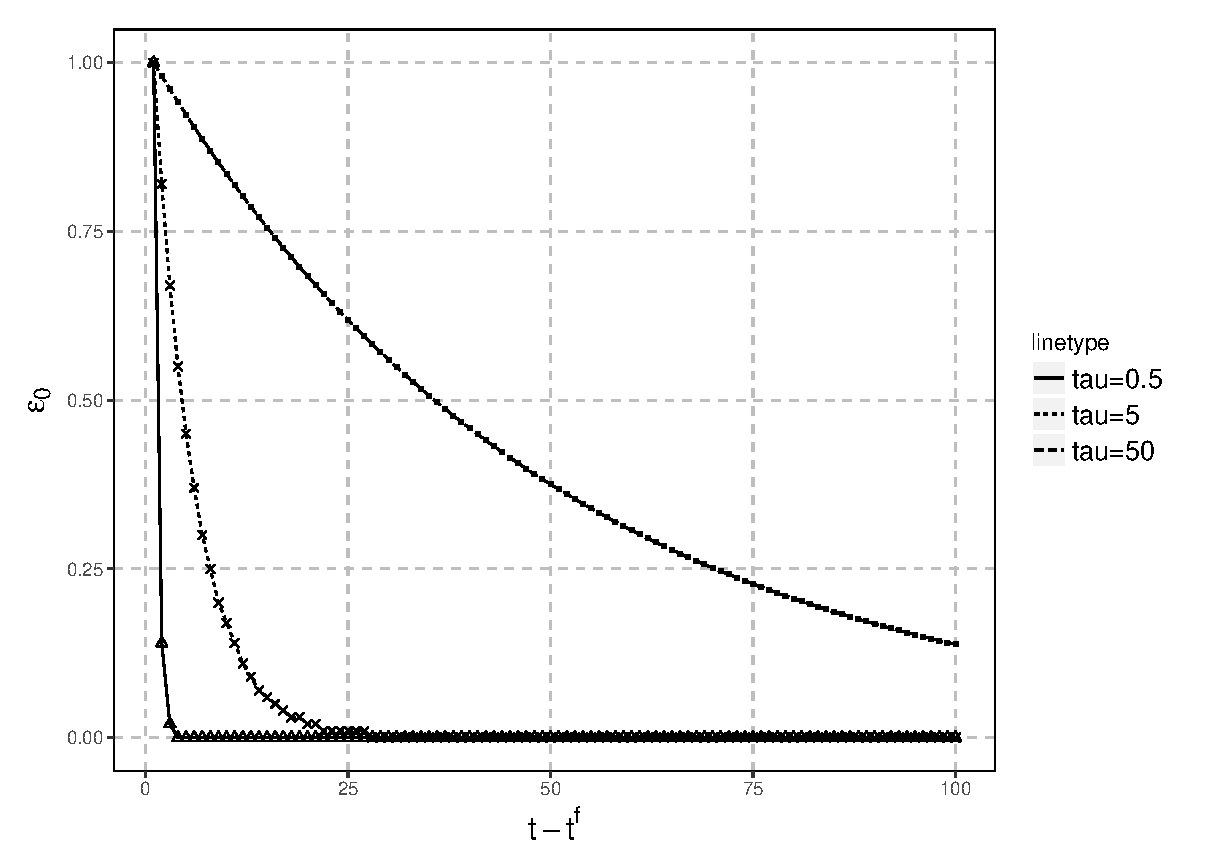
\includegraphics[width=0.8\textwidth]{fig/fmridti/potential_kernel.eps}
	\caption{Plot of the PSP trace $\epsilon_0$ as a function of $t-t^f$. This figure plots the PSP simulation for different $\tau_m$.}
	\label{fig:PSP}
\end{figure}




\subsubsection{Temporal Integration of PSP Kernels and Conditions for Spike Emission}
Under the SRM model, the PSPs evoked by the pre-synaptic neurons are temporally integrated to activate the spiking neuron. The overall contribution of the pre-synaptic spikes elicited by the pre-synaptic neurons $j$ at any time $t$ is given as \equationname \ref{eq:SRM0} describing the SRM model:


\begin{equation}
v_i(t)=v_{rest}+\sum_{j\in \Tau_i }w_{ji}\sum_{t_j^f\in F_j}\epsilon_0(t-t_j^f)
\label{eq:SRM0}
\end{equation}

The temporal summation is a double summation operation. The inner sum adds up the PSP contributions due to the firings $t_j^f\in F_j$ of one pre-synaptic neuron. The outer sum adds up the PSP contributions of all the pre-synaptic neurons $j\in \mathcal{T}_i$ connected to neuron $i$. \equationname \ref{eq:SRM0} describes the membrane potential (activation state) $v_i$ of a spiking neuron $i$ can be calculated by adding the resting potential term and the temporal PSP sum. Each incoming spike perturbs the value of $v_i$ and if, after the summation of the inputs, the membrane potential reaches the threshold $v_{thr}$ then an output spike is generated. The firing time is given by the condition $v_i(t_i^f)>=v_{thr}$. After a neuron fires the neurons' membrane potential is reset to $v_{rest}$. In standard NeuCube implementations, the inner sum is generally set to $1$. By setting the inner sum to $1$, NeuCube only uses the information of present instance and forgets the influence of historical spike-trains, thus demonstrating minimal memory in the neuron model. However, any instance of the usage of NeuCube based architecture in this thesis uses the historical information with a preset hyperparameter controlling the memory horizon.   

\subsubsection{Refractory Period}
After emitting the spike, a spiking neuron enters a period of quietness known as the refractory period. During this period, the membrane potential remains unaffected by incoming spikes. The refractory behaviour can be mathematically achieved by setting the membrane potential to a infinitely low value. In the SRM model the neuron behaviour under the influence of refractoriness depends only on the last firing moment leading to a short-term memory in the neuron. In the literature, the refractory period is described by absolute and relative refractory period. During the absolute refractory period, the neurons do not accumulate membrane potential and hence cannot fire. During the relative refractory period, it can be relatively difficult but not impossible to fire the neuron. In this current implementation, an absolute refractory period for the sake of simplicity has been used here. The absolute refractory period of a neuron is specified by the hyperparameter $\eta_{thr}$. 

The modified SRM neuronal dynamics of NeuCube is formalised by \equationname \ref{eq:SRM_neucube}. The modifications of the canonical SRM model can be observed in: (1) the implementation of the PSP kernel which outputs a unit pulse at the time neuron $i$ receives a spike from neuron $j$; (2) the implementation of refractoriness, where the membrane potential is set to negative infinity during the period $\eta_{thr}$ after neuron $i$ fires a spike at time $t_i^f$.
\begin{equation}
\begin{matrix}
\displaystyle v_i(t)=v_{rest}+\sum_{j\in \Tau_i }w_{ji}\sum_{t_j^f\in F_j}\epsilon_0(t-t_j^f)+\eta(t-t_i^f) \\

\epsilon_0(t-t_j^f)=\left\{
\begin{array}{@{}cc@{}}
1, & \text{if}\ t-t_j^f=0 \\
0, & \text{otherwise}
\end{array}\right. \\

\eta(t-t_i)=\left\{
\begin{array}{@{}cc@{}}
-\infty, & \text{if}\ t-t_i^f<\eta_{thr}\\
0, & \text{otherwise}
\end{array}\right.

\end{matrix}
\label{eq:SRM_neucube}
\end{equation}

\begin{figure}
	\centering
	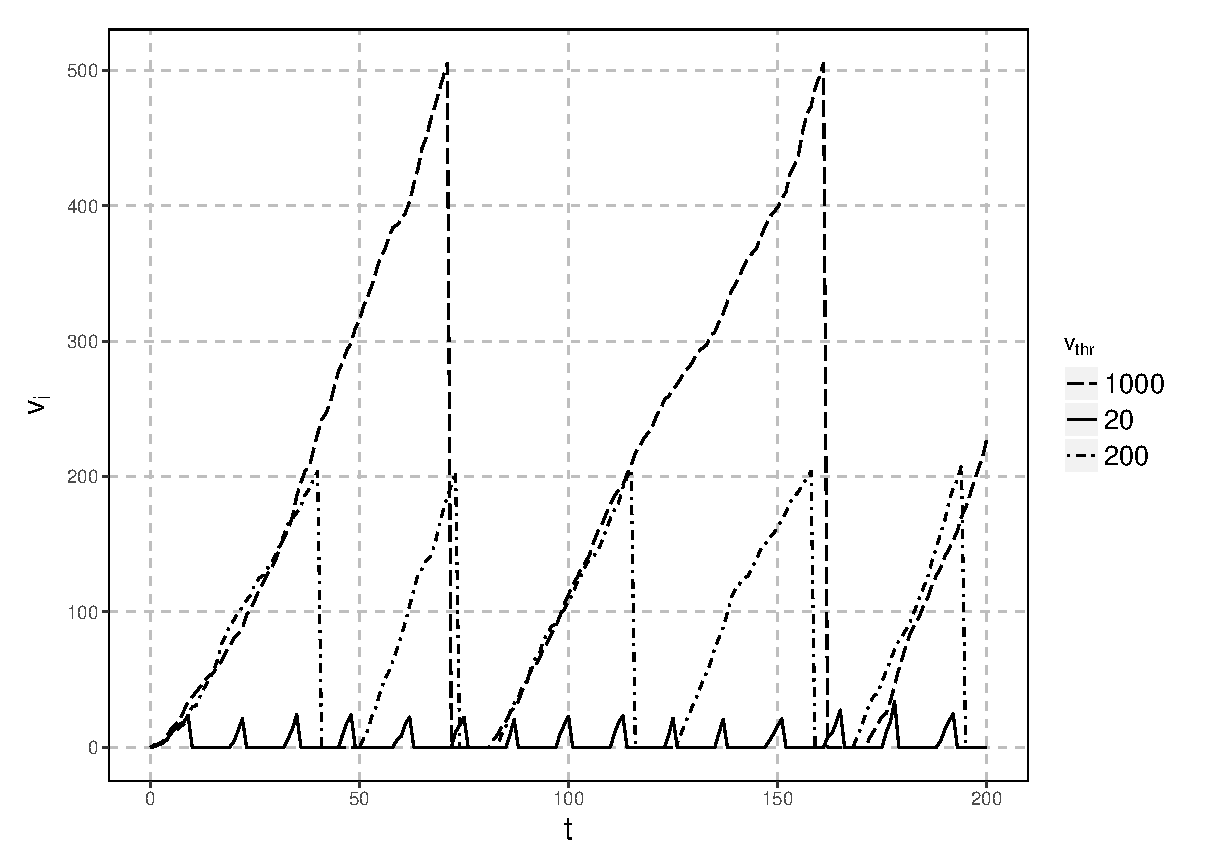
\includegraphics[width=0.8\linewidth]{fig/fmridti/membrane_potential.eps}
	\caption{Plot of the membrane potential traces($v_i$) of a neuron $i$ simulated over $T=200$ time points using the SRM model. For the simulations, $3$ predecessor neurons were connected to a spiking neuron. The spike data from the predecessor neurons are sampled randomly from uniform random distribution. The $\eta_{thr}$ for the spiking neuron was set to $10$. Each of the three $v_i$ traces correspond to a preset $v_{thr}$ mentioned in the label.}
	\label{fig:SRM}
\end{figure}

\figurename \ref{fig:SRM} shows a plot of three simulations of a spiking neuron for $200$ discrete times with random spike inputs. Each simulation uses a preset $v_{thr}$. At the beginning of the simulation, the neuron is in a resting state $v_{t=0}=v_{rest}$. With the arrival of spikes, the membrane potential increases in a linear fashion and when sufficiently stimulated (sufficiency is determined by $v_{thr}$), the neuron spikes, and then goes back to the resting state. At this point, the neuron is said to be in a refractory state. The neuron stays in this state for a predetermined period $\eta_{thr}$ and then goes back to a non-refractory state.  

\subsection{Unsupervised Weight Adaptation in SNNc}

The unsupervised weight adaptation mechanism in the SNNc is an extremely important aspect of the dynamics. In a neural network paradigm, learning or plasticity is achieved through the synaptic strength updates of the network. The learning behaviour of the SNNc can be explained using the learning model of a single spiking neuron. Considering the single neuron architecture in \figurename \ref{fig:neuron_architecture}, the unsupervised learning problem is to formalise a scheme of updating the weights $W$ of the network by $\Delta W(t)$ over the simulation time $T$. The NeuCube SNNc has employed numerous variations of temporally asynchronous forms of Hebbian learning in different implementations. 

\subsubsection{STDP} 
\label{subsec:STDP}
\begin{figure}
	\centering
	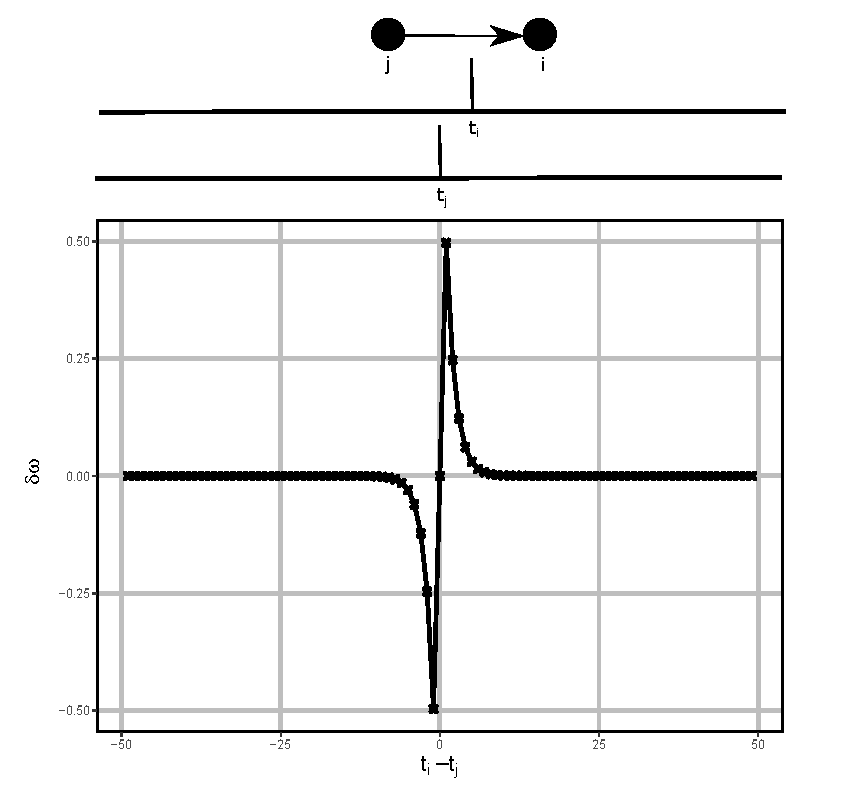
\includegraphics[width=0.8\linewidth]{fig/largesnn/STDP.eps}
	\caption{Plot showing the functional dependence of the spike-time dependent plasticity learning rule. The STDP function shows the change of synaptic weights $\Delta w$ as a function of difference in post and pre-synaptic spike-time difference.}
	\label{fig:STDP_exp1}
\end{figure}


STDP is a temporally asymmetric form of Hebbian learning induced by temporal correlations between the spike-timings of pre- and post-synaptic neurons \citep{song2000competitive}. As with other forms of synaptic plasticity, it is thought to underlie learning and memory in the brain, as well as the development and refinement of neuronal circuits during the development of the brain. With STDP, repeated pre-synaptic spike arrival, a few discrete times earlier to post-synaptic firing leads to Long Term Potentiation (LTP) of a synapse, whereas repeated spike arrival after post-synaptic spike generation leads to Long Term Depression (LTD) of the same synapse. The synaptic weight changes as a function the relative firing-time of the pre- and post-synaptic neurons, also known as the STDP learning window \citep{gerstner2002spiking}. The overall significance of STDP lies in the ability of a spiking neuron to discriminate between, and then integrate, temporally significant inputs and transforming that to meaningful output, even though the actual meaning is not strictly known by the neuron \citep{markram2011introducing}. Networks that employ STDP operates as palimpsests, \emph{i.e.} older stimuli are forgotten gradually to make room for new ones.

\citet{gerstner1996neuronal, song2000competitive} formalised the mathematical model of STDP learning as per \equationnames \ref{eq:stdp1} and \ref{eq:stdp2}. Symbols $j$ and $i$ are used to indicate pre- and post-synaptic neurons. In STDP learning, the dynamic change of weight $\Delta w$ is estimated using a learning window function $W(\cdot)$. The learning window takes historical pre-synaptic firing times $\{t_j^1 \cdots t_j^f\}$ and post-synaptic firing times $\{t_i^1\cdots t_i^g\}$ as input and calculates the LTP and LTD traces. These historical firing times are nothing but indices of a historical spike sequence. For example, a historical spike sequence $[01001011]$ can be rewritten as sequence of spike-time indices $t^f :=\{1, 4, 6, 7\}$. Exponential decay functions are a popular choice for the learning window and \equationname \ref{eq:stdp2} is a good choice of the learning window function. The $\kappa_+$ and $\kappa_-$ parameters control the maximum LTP and LTD update respectively and $\kappa_-=\kappa_+=1$ is a good choice to keep the bounds of weight update between $[-1, 1]$. From \equationname \ref{eq:stdp2}, it can be observed that the polarity of $(t^g_i-t^f_j)$ defines the polarity of $\Delta w_{ji}$. This is Hebbian model of causal relationship where synapses are rewarded positively (strengthened) for causal firing ($i$ fires later than $j$ \emph{i.e.} firing of $i$ is caused by firing of $j$) and penalised (weakened) for non-causal firing. However, \equationnames \ref{eq:stdp1} and \ref{eq:stdp2} describes a batch update scheme and requires modification for on-line learning in the SNNc. \citet{sjostrom2010spike} proposed a modified on-line STDP update rule. In the on-line setting, $\Delta w_{ji}$ is calculated every time neuron $i$ fires a spike or receives a spike from neuron $j$. \equationname \ref{eq:stdp_online} formalises the weight update rule for on-line mode. The first term in the right hand side of \equationname \ref{eq:stdp_online} corresponds to the LTP update and is calculated when neuron $i$ fires a spike at time $t$. The second term is the LTD update and is calculated when neuron $i$ receives a spike from neuron $j$ at time $t$. Both the batch and on-line formalisations of STDP learning are extended from \citep{sjostrom2010stdp} which discusses the properties of the STDP learning model extensively. \figurename \ref{fig:STDP_exp1} shows the plot of the STDP learning function where the $\Delta w$ in quadrants I and III correspond to LTP and LTD respectively.
\begin{equation}
\Delta w_{ji}:=\sum_{f}\sum_{g} W(t^g_i-t^f_j)
\label{eq:stdp1}
\end{equation}
\begin{equation}
W(s) :=
\left\{
\begin{array}{ll}
\kappa_+\exp(-s)  & \mbox{if } s > 0 \\
-\kappa_-exp(-s) & \mbox{if } s < 0
\end{array}
\right.
\label{eq:stdp2}
\end{equation}


\begin{equation}
\Delta w_{ji}(t) := \sum_f \kappa_+\exp(-(t-t_j^f))-\sum_g \kappa_- \exp(-(t-t_i^g))
\label{eq:stdp_online}
\end{equation}

It is evident from the discussion above that the STDP learning rule enhances or depletes the synaptic strength of the connections, based on the relative coincidence of the spikes. This behaviour mimics the ability of the biological neurons to encode information by detecting the occurrence of temporally close but spatially distributed input signals and thus incorporating spatio-temporal information in the model.

\subsubsection{Modified STDP in NeuCube} 
\label{subsec:mod_STDP}
\begin{figure}
	\centering
	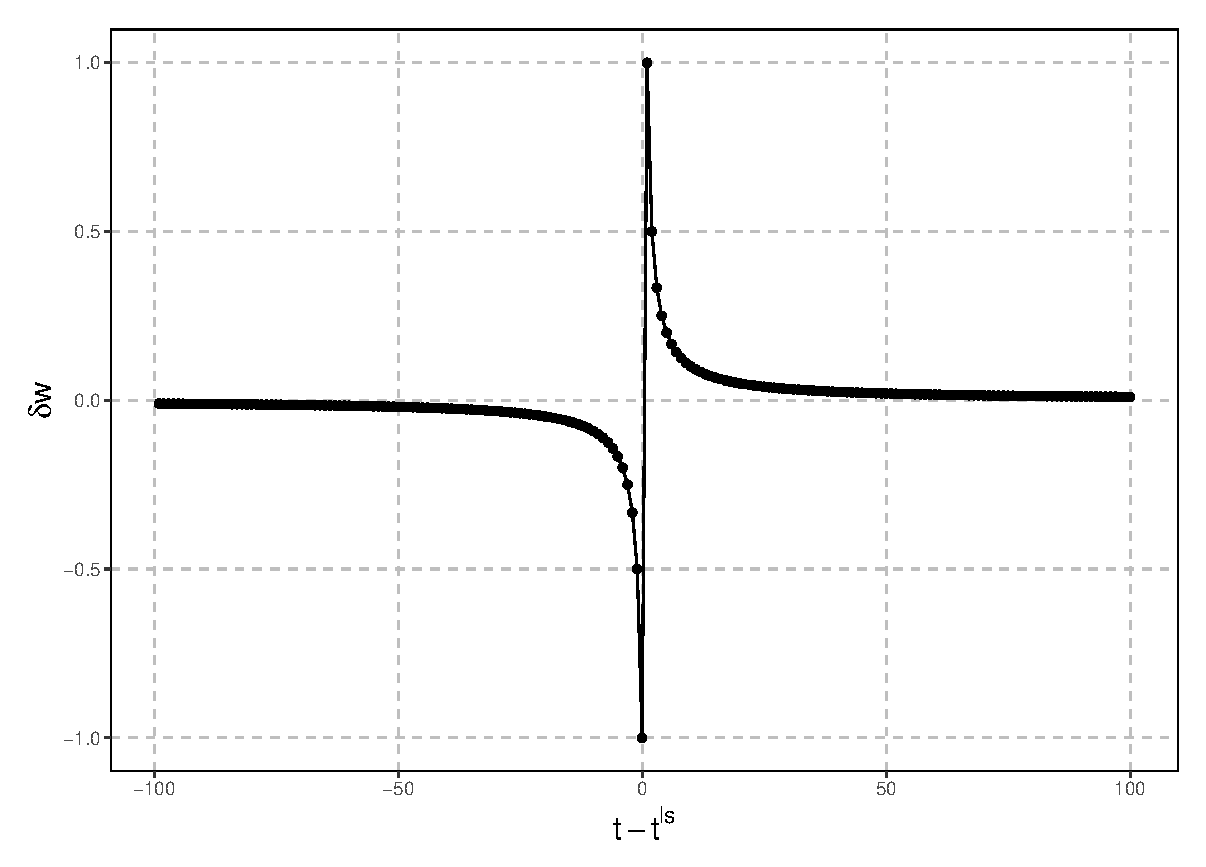
\includegraphics[width=0.8\linewidth]{fig/largesnn/mod_STDP.eps}
	\caption{Plot of modified spike-time dependent plasticity learning rule implemented in SNNc learning algorithm. The STDP function shows the change of synaptic weights $\Delta w$ as a function of difference in last and present spike-time difference.}
	\label{fig:mod_STDP_exp}
\end{figure}


The standard NeuCube implementation uses a modified form of the STDP learning algorithm. The modification mainly relates to when and which neurons are updated. The contrast between STDP and modified STDP are:

\begin{enumerate}
	\item As opposed to the STDP learning, in modified STDP learning, synaptic updates are only performed when a neuron $i$, fires a spike, and not when it receives a spike.
	\item When a neuron $i$ fires, both pre- and post-synaptic strengths are updated. The pre-synaptic connections are strengthened and post-synaptic connections are depleted. 
\end{enumerate}

The weight update rule can be formalised by \equationnames \ref{eq:mod_stdp1} and \ref{eq:mod_stdp2}, where $t^{ls}$ is the last spike time of a neuron and $t$ is the current time instance. It is quite evident that the smaller the difference between $t$ and $t^{ls}$ the more significant the weight update is. This weight update rule also implies that enhanced importance is given to faster firing rate. $\kappa_+$ and $\kappa_-$, referred to as learning rate in the NeuCube literature, control the upper and lower bound of $\Delta w$ similar to STDP. \figurename \ref{fig:mod_STDP_exp} shows the functional dependence plot of the modified STDP learning. It is quite evident from the plot that the weight update curve is very similar to the STDP weight update rule. The difference, however, lies in the functional dependence as discussed. 
   

\begin{equation}
	\Delta w_{ik}(t)=\frac{\kappa_+}{t-t^{ls}_j+1}
	\label{eq:mod_stdp1}
\end{equation}

\begin{equation}
	\Delta w_{ji}(t)=-\frac{\kappa_-}{t-t^{ls}_k+1}
	\label{eq:mod_stdp2}
\end{equation}

\begin{algorithm}
	\begin{algorithmic}[1]
		\STATE \textbf{input}: $G=\{M, C, W\}$, $D_{seq}\in \{0,1\}^{|N|\times |T|}$, $\{hyperparameters:=v_{thr}, \eta_{thr}, \kappa\}$
		\STATE \textbf{output}: $O_{seq} \in \{0, 1\}^{|M|\times |T|}$
		
		\FORALL {$t \in T$}
			\STATE initialise $C_{learn}\leftarrow\{\}$
			\FORALL {$i \in Q$}
				\STATE find firing (at $t-1$) pre-synaptic neurons, $J_i^{spk(t-1)}$
				\STATE set $C_i^{ltd}\leftarrow (J_i^{spk}, i)$
				\STATE set $C_{learn}+\leftarrow C_i^{ltd}$
				\STATE simulate neuron $i$ as per \equationname \ref{eq:SRM_neucube}
				\IF{$i$ fires}
					\STATE set $O_{seq}[i, t+1]\leftarrow 1$
					\STATE find pre-synaptic neurons, $J_i^{spk(t)}$
					\STATE set $C_i^{ltp}\leftarrow (J_i,i)$
					\STATE set $C_{learn}+\leftarrow C_i^{ltp}$
				\ENDIF
			\ENDFOR
			\FOR {$c_{ji}\in C_{learn}$}
				\STATE calculate $\Delta w_{ji}(t) \leftarrow \sum_f \kappa_+\exp(-(t-t_j^f))-\sum_g \kappa_- \exp(-(t-t_i^g))$
				\STATE update $w_{ji}+\leftarrow \Delta w_{ji}$
			\ENDFOR
		\ENDFOR
		\caption{STDP based SNNc unsupervised learning algorithm}
		\label{alg:unsup_stdp}
	\end{algorithmic}
\end{algorithm}

\subsection{Formal Description of SNNc Unsupervised Learning Algorithm}
\label{sec:neucube_snnc_learning}
\begin{algorithm}
	\begin{algorithmic}[1]
		\STATE \textbf{input}: $G=\{M, C, W\}$, $D_{seq}\in \{0,1\}^{|N|\times |T|}$, $\{hyperparameters:=v_{thr}, \eta_{thr}, \kappa\}$
		\STATE \textbf{output}: $O_{seq} \in \{0, 1\}^{|M|\times |T|}$
		
		\FORALL {$t \in T$}
		\STATE initialise $C_{learn}\leftarrow\{\}$
		\FORALL {$i \in Q$}
		\STATE find firing (at $t-1$) pre-synaptic neurons, $J_i^{spk(t-1)}$
		\STATE simulate neuron $i$ as per \equationname \ref{eq:SRM_neucube}
		\IF {$i$ fires}
		\STATE set $O_{seq}[i, t+1]\leftarrow 1$
		\STATE find pre- and post-synaptic neurons $J_i^{spk(t)}$ and $K_i^{spk(t)}$
		\STATE set $C_i^{ltp}\leftarrow (J_i^{spk(t)}, i)$ and $C_i^{ltd}\leftarrow (i, K_i^{spk})$
		\STATE set $C_{learn}+\leftarrow C_i^{ltp}$ and $C_{learn}+\leftarrow C_i^{ltd}$
		\ENDIF
		\ENDFOR
		\FOR{$\{c_{ji}, c_{ik}\} \in C_{learn}$}
		\STATE calculate $\Delta w_{ji}\leftarrow \frac{\kappa}{t-t_j^{ls}+1}$ and $\Delta w_{ik}\leftarrow -\frac{\kappa}{t-t_k^{ls}+1}$
		\STATE update $w_{ji}+\leftarrow \Delta w_{ji}$ and $w_{ik}+\leftarrow \Delta w_{ik}$
		\ENDFOR
		\ENDFOR
		\caption{Modified STDP based SNNc unsupervised learning algorithm}
		\label{alg:unsup_mod_stdp}
	\end{algorithmic}
\end{algorithm}

A classical implementation of the SNNc unsupervised learning algorithm is formally presented in \algorithmname \ref{alg:unsup_mod_stdp}. This algorithm uses the modified STDP learning described in Section \ref{subsec:mod_STDP}. The goal of the learning algorithm is to continuously input data sequence $D_{seq}$ in the form of spikes and simulate the network $G$ in a way that the synaptic strengths $W$ of the network are updated over time $T$ to learn poly-synchronous relationships across space and time. The hyperparameters for neuron simulation ($v_{thr}, \eta_{thr}$) and learning ($\kappa$) are also input into the learning algorithm. At the end of the simulation, the algorithm outputs the  spike sequence $O_{seq}$. The simulation of G is performed at every time instance $t \in T$ and is described within the loop between line $3$ and $19$ in \algorithmname \ref{alg:unsup_mod_stdp}. At every time instance, an empty variable $C_{learn}$ is initialised, which stores over the subsequent steps, a subset of connection identities ($C_{learn}\subset C$) for the synaptic strength updates. The simulation is then performed in two subsequent phases. In the first phase (line $5$ to line $14$), all the spiking neurons $Q$ are simulated based on the spiking neuron model. In NeuCube, the neuron simulations are done following \equationname \ref{eq:SRM_neucube}. In NeuCube, pre- ($J_i^{spk(t)}, i$) and post-synaptic ($i, K_i^{spk(t)}$) connections of the spiking neurons that fire at time instance $t$ are candidates for weight evolution. These connections are stored in $C_{learn}$ for update. The second step (line $15$ to line $18$) is the learning stage. During the learning stage, the connections $C_{learn}$ are updated according to the learning rule, which in case of \algorithmname $\ref{alg:unsup_mod_stdp}$ is the modified STDP learning rule. In addition, \algorithmname \ref{alg:unsup_stdp} also presented the SNNc unsupervised learning algorithm using the canonical STDP learning rule described in Section \ref{subsec:STDP}. A careful comparison between the two algorithms reveal that the synaptic strength update in modified STDP is drastically different from canonical STDP in regards to when and what synapses are updated.    

\subsubsection{Considerations for Parallelisation}
Neural networks are generally considered as a massively parallel problem, \emph{i.e.}, the computations are simultaneous rather than sequential in layers of a typical neural network. Therefore, the divide and conquer type of parallelisation construct can be very easily achieved in neural networks by using the map and reduce paradigm of functional programming. However, by observing the characteristics of the SNNc learning algorithm, there does not seem to be a clear parallelisation approach. This is caused by the recurrence present as the output of the neurons in the SNNc layer, in the form of spike sequences which are recurrently fed back to other neurons creating a neuron level dependency over space and time. Therefore, although it is very tempting to merge the learning step and the neuron simulation step across the spiking neurons together, the asynchronous nature of the updates deems it an extremely hard parallelisation problem. The system clock driven computational simulation at the moment is clearly different from the clock precise parallelised scheme in the brain.    

\section{Analysis of the Data Structure Representations of SNNc} 
In this Section, focus of attention will be on the SNNc network structure representation $G$ in light of \algorithmname \ref{alg:unsup_mod_stdp}. The overall objective of the network structure representation analysis is guided by the objective to improve the computation and storage load of the algorithm as the unsupervised learning mechanism evolves the network over time. This work specifically looks into the storage and time complexity of the algorithm with increasing numbers of neurons in the network. During the iterative simulation process, the connections and the weights of the network are accessed very frequently. Parts of the SNNc network are accessed specifically in lines $6, 10-12$ and $15-17$. The access to the network is theoretically a search operation within the search space $C$ for information on specific neuron identities. In particular, the algorithm needs to access the immediate neighbours of a given neuron $i$. These are the pre- and post-synaptic neurons $J_i^{spk}$ and $K_i^{spk}$. A data structure that is used for representing the network must, therefore, provide fast accessibility of neighbouring nodes. As an additional constraint, the present work focuses on the algorithmic implementation of a general purpose von-Neumann architecture computer (as opposed to the implementation on a neuromorphic hardware \citep{scott2015thesis} setup), designed for  commodity consumption. Therefore, storage space and computing capacity are of course constrained and an optimum data structure representation should be storage- and time-efficient. For the current experiments, a general purpose PC running a 64 bit Windows 7 enterprise operating system was used; one that had 16GB RAM, Intel Core i5 processor with 3.20 GHz clock speed. The implementations of \algorithmname \ref{alg:unsup_mod_stdp} was done in Matlab version R2014b.

In the Matlab based prototype and testing version of NeuCube, an adjacency matrix was used to store the connection structure $C$. According to graph theory, an adjacency matrix is defined as a square matrix $C$ of order $M$ (number of neurons) where 1 represents an existing edge between the two vertex indices. The edges correspond to the connections, and the vertices are the neuronal unique identifiers. In the present implementation, a second adjacency matrix is needed to store the weights $W$ in order to avoid confusion between the existence of an edge and the weight values themselves. \figurename \ref{fig:adj_mat} shows an example of an adjacency matrix. Since all values in an adjacency matrix can be directly accessed by using the corresponding neuron IDs as indices, this data structure is extremely fast. However, due to the nature of storing all relations between vertices, the storage had grown at a squared rate, and it also showed to be the most storage demanding option when compared to other data structures. 
\begin{figure}
	\centering
	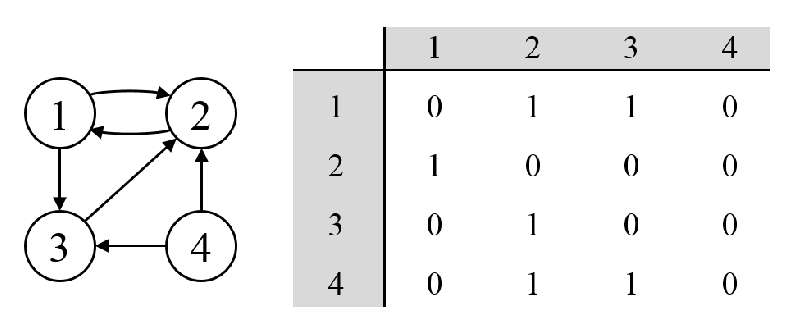
\includegraphics[width=0.5\linewidth]{fig/largesnn/adj_matrix.eps}
	\caption{Example of the adjacency matrix representation.}
	\label{fig:adj_mat}
\end{figure}

The second option that was investigated was an edge-weight table. An edge-weight table stores the connection and their weights in a simple look-up table with each row containing a pair of neuron indices (identities) $i$ and $j$, and the weight of the connection between them, as shown in \figurename \ref{fig:ijv_tab}. This edge-weight table used far less storage than the adjacency matrix; however, it was also considerably slower, because in order to access a connection between a pair of neurons, the whole table had to be searched, which meant an average time complexity of $O(\frac{1}{2}c)$. Ordering the table by neuron $i$ to use it as an index could to some extent alleviate the problem for finding post-synaptic neurons, but not for pre-synaptic neurons, since in that case only neuron $j$ was given. Therefore, this data structure is sub-optimal in regards to computation time especially in case of larger networks.

\begin{figure}
	\centering
	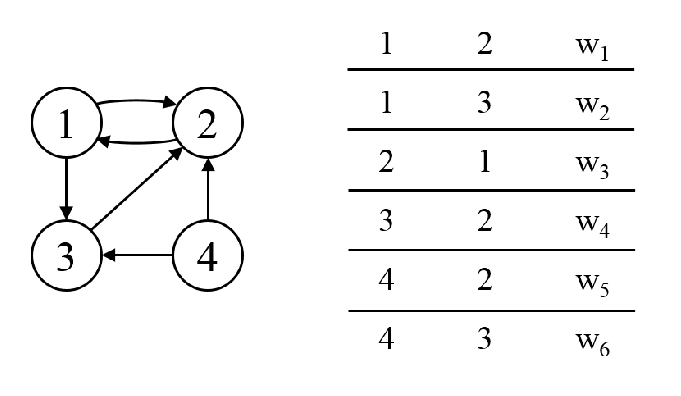
\includegraphics[width=7cm]{fig/largesnn/ijv_table.eps}
	\caption{Example of the edge-weight table representation.}
	\label{fig:ijv_tab}
\end{figure}

The third data structure was an adjacency forward list. In graph theory, this is a list of vertices in which each entry contains a sub-list of neighbouring vertices. An example for an adjacency forward list is depicted in \figurename \ref{fig:adj_list}. In terms of storage space, the adjacency list, like the edge-weight table, is considerably smaller than the adjacency matrix as it only stores the connections. Compared to the edge-weight table, the adjacency forward list saves space by listing all neurons connected to neuron $i$ in an indexed list (the index being neuron $i$) instead of repeating the index for every connection. However, for \algorithmname \ref{alg:unsup_mod_stdp}, a second adjacency forward list was needed to store the weight values of the connections, which is why this data structure uses slightly more storage space than the edge-weight table in the experiments. In terms of temporal performance, the adjacency forward list was also very similar to the edge-weight table in that it was faster to access post-synaptic connections due to indexing than looking up pre-synaptic connections where all sub-lists had to be searched. However, the indexing mechanism of the adjacency forward list provides a significantly faster look-up of post-synaptic connections than the edge-weight table. For these reasons, the adjacency forward list is overall expected to scale up best for a larger number of neurons, compared to the edge-weight table and the adjacency matrix.

\begin{figure}
	\centering
	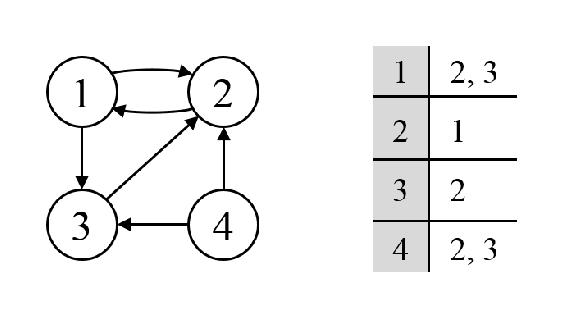
\includegraphics[width=6.2cm]{fig/largesnn/adj_list.eps}
	\caption{Example of the adjacency forward list representation.}
	\label{fig:adj_list}
\end{figure}

Taking into consideration that the adjacency forward list is a very storage-efficient data structure and that its main bottleneck for temporal performance is the look-up of pre-synaptic indices, a decision was made to add a second adjacency list called an adjacency backward list to the structure to represent the connections from the opposite perspective, thus making the neuron at the end of the connection (neuron $j$) the index of this second list. A schema of this approach is shown in \figurename \ref{fig:fw_bw_adj_list}. This “backwards” indexing mechanism caused a significant decrease of the algorithm's execution time, because it effectively reduced the time complexity of the data structure to $O(1)$ for finding the right pre-synaptic and post-synaptic indices. In comparison with the other data structures, the adjacency forward-backward list was now the best alternative for representing the SNNc network. \tablename \ref{tab:complexity} gives a comparative overview of the theoretical complexities in regards to time and storage with the different data structures discussed here. The complexities are measured by $n$ and $c$ referring to the neuron count and connection count respectively. The relationship between $n$ and $c$ can be represented by $c=\alpha\times n^2$, where $\alpha\in [0, 1]$ is the degree of sparseness. All of the present experiments have used $\alpha=0.02$. 

\begin{figure}
	\centering
	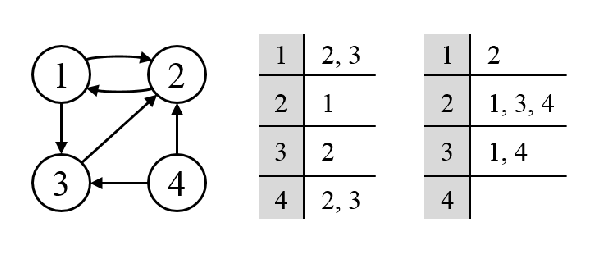
\includegraphics[width=7.8cm]{fig/largesnn/adj_bw_list.eps}
	\caption{Example of the adjacency forward-backward list representation.}
	\label{fig:fw_bw_adj_list}
\end{figure}

\begin{table}
	\centering
	\caption{Comparison of time and storage complexity for different data structures.}
	\label{tab:complexity}
	\resizebox{\textwidth}{!}{\begin{tabular}{@{}|l|c|c|c|c|c|@{}}
		\toprule \toprule
		\multirow{2}{*}{data structure} & \multicolumn{1}{c|}{\multirow{2}{*}{connection type}} & \multicolumn{3}{c|}{time} & \multirow{2}{*}{storage} \\ \cmidrule(lr){3-5}
		& \multicolumn{1}{c|}{} & \multicolumn{1}{c|}{worst} & average & best &  \\ \midrule
		adjacency matrix & all & \multicolumn{3}{c|}{$O(1)$} & \multicolumn{1}{c|}{$S(n^2)$} \\ \midrule
		edge-weight table & all & $O(c)$ & $O(\frac{1}{2}c)$ & $O(1)$ & $S(c)$ \\ \midrule
		\multirow{2}{*}{adjacency forward list} & pre-synaptic & \multicolumn{1}{c|}{$O(c)$} & $O(\frac{1}{2}c)$ & $O(1)$ & \multicolumn{1}{c|}{\multirow{2}{*}{$S(2\times c)$}} \\ \cmidrule(lr){2-5}
		& post-synaptic & \multicolumn{3}{c|}{$O(1)$} & \multicolumn{1}{c|}{} \\ \midrule
		adjacency forward-backward list & all & \multicolumn{3}{c|}{$O(1)$} & \multicolumn{1}{c|}{$S(3\times c)$} \\ \bottomrule \bottomrule
	\end{tabular}}
\end{table}

The findings from the theoretical analysis of the structures' complexity could be verified through the present experimental results. For the experiments, a benchmark EEG dataset was used. The dataset consisted of EEG data measuring brain signals during a task of wrist movement. The wrist movements were categorised into upward, downward, and central directions. This task was performed on a single subject and EEG data was sampled from $14$ channels at a sampling rate of $128$ Hz while the subject performed the task. $20$ independent trials of one second duration were collected while the subject performed each movement task. $14$ of the $1485$ neurons in the reservoir were randomly chosen as input neurons for the EEG channels. A network with a highly sparse connectivity ($\approx 2\%$ of all possible connections) was initialised randomly for every experiment. The value of two per cent was chosen because this was the average amount of connections used typically during experiments.

\figurename \ref{fig:storage_comp} shows the comparison of storage required in megabytes by each of the data structures. The graph itself is dependent on the number of neurons in the SNNc (between $0$ and $70,000$ for the storage, and between $500$ and $3,500$ for the execution time). When it was decided that the number of neurons should be increased further, all values above $80,000$ neurons for the adjacency matrix and above $120,000$ neurons for the sparse matrix had to be excluded, due to the above discussed technical restrictions in the experimental setup. In addition, it became difficult to distinguish between the curves, especially in the lower regions of the graph.

\begin{figure}
	\centering
	\includegraphics[width=0.8\linewidth]{fig/largesnn/storage.eps}
	\caption{Storage space comparison of different data structures with increasing number of neurons.}
	\label{fig:storage_comp}
\end{figure}

\begin{figure}
	\centering
	\includegraphics[width=0.8\linewidth]{fig/largesnn/time.eps}
	\caption{Execution time comparison of different data structures with increasing number of neurons.}
	\label{fig:time_comp}
\end{figure}

It is clearly visible that the adjacency matrix has the steepest increase of storage space needed. The other three data structures are relatively similar in their development, with the edge-weight table growing slowest. It was interesting to see that the curve of the sparse matrix was very close to the one of the adjacency list, which indicates that the internal representation of a sparse matrix in Matlab is similar to an adjacency list. \figurename \ref{fig:time_comp} shows the results of comparing the execution time of the data structures. For the comparison of execution times, the curve of the edge-weight table showed its disadvantage as it increases near exponentially. Thus, another graph representation without the edge-weight table was created. This showed that the adjacency list was considerably slower than the matrices and the adjacency backwards list.

These experimental results verify the previous theoretical analysis. The most promising data structure for representing an SNNc network having a large number of neurons in the NeuCube SNN is the adjacency list with backwards indexing due to its constant complexity in terms of execution time of the algorithm, and linear storage growth with increasing connection density.


\subsection{Large-scale Unsupervised Learning of SNNc Using the Adjacency Forward-backward List}

\begin{figure}
	\centering
	\includegraphics[width=0.8\linewidth]{fig/largesnn/spike_simulation.png}
	\caption{Snapshot of the spike activity at a time instant inside the SNNc.}
	\label{fig:spike_simulation}
\end{figure}

\begin{figure}
	\centering
	\includegraphics[width=0.8\linewidth]{fig/largesnn/connection_simulation.png}
	\caption{Strongest connections learned by the SNNc at the end of SNNc simulation.}
	\label{fig:connection_simulation}
\end{figure}

As a conclusion of the current experimental results, it seemed evident that the adjacency forward-backward list data structure representation is the most economic in regards to storage and temporal complexity. To further demonstrate this, the NeuCube SNNc learning algorithm in Matlab capable of using the adjacency forward-backward list data structure was implemented (see Appendix \ref{chap:app_SNNc_unsupervised} for the Matlab programme). In order to test the efficiency of the implementation on a much larger scale, \algorithmname \ref{alg:unsup_mod_stdp} was run on a SNNc consisting of $241,606$ neurons taking the same EEG input data described earlier. The SNNc was simulated to mimic a brain with neural cells in the order of $10^6$ and connections in the order of $10^{10}$. The spatial coordinates of the neurons were obtained from the xjView \citep{cui2011xjview} software and resembled the spatial distribution of the human brain based on the MNI coordinate system. \figurename \ref{fig:spike_simulation} shows a snapshot of spiking patterns at a certain time instance during the unsupervised learning simulation. The ripple like behaviour of the liquid state within the SNNc can be clearly observed in the network. The ripple effect in the SNNc is of course clearly visible in a dynamic simulation environment. \figurename \ref{fig:connection_simulation} shows the strongest connections formed in the brain-like network as a result of the unsupervised learning.

\section{Considerations for Modularity and Heterogeneity: Towards Graph Based Software Design of SNNc}
In the last Section, the considerations of scalability in regards to the size of the SNNc was discussed. At this point, it is critical to mention that apart from the large size, biological brains are considerably modular and heterogeneous. The theory of modularity suggests that there are functionally specialised regions in the brain that are domain specific for different cognitive processes. The brain is often represented as a network of interconnected, dynamically interacting elements. Cognitive processes are thought to result from the integration of neuronal processing distributed across these complex networks at different temporal and spatial scales. Several graph theory based methods \citep{sporns2016modular, nicolini2016modular} have been proposed in analysing the modularity and heterogeneity in the brain.

The idea of modularity and heterogeneity is of major importance for the neuromorphic inspirations of the SNNc architecture design. Heterogeneity and modularity is observed not only in the brain but is quite prevalent in a broad range of networks, such as groups in social networks, ensembles of interacting proteins or coregulated genes in cellular network. These clusters or groups of items have homogeneous property behaviours within the group, and vary considerably between the groups across the network. 

The objective of this Section was to design algorithmic or implementation improvements to facilitate heterogeneity and modularity in the SNNc. Let us revisit the implementation of unsupervised learning algorithms (see Appendix \ref{chap:app_SNNc_unsupervised}). The functional style of implementation constrains the ability to inject heterogeneity into the network, especially if one considers designing networks with varieties of neurons, synapses, learning behaviour etc. 

The basic concept behind the template method design pattern is relatively simple. Generally abstract classes are created representing necessary steps for a general algorithm operation. An instantiation of the template (class) then implements these steps with necessary extension. In \algorithmname \ref{alg:unsup_mod_stdp}, the network $G$ is represented by the tuple $<M, C, W>$. $M$ is a list of neuron identifiers and serves no purpose other than storing the identifiers. The code for neuron simulation is integrated within the network simulation programme and is independently treated compared to $M$. Additionally, weights are modelled independently of the connections in \algorithmname \ref{alg:unsup_mod_stdp}. 

In order to overcome these shortcomings, the SNNc network in the graph based design is constructed as a directed graph data structure. The graph based architecture that was designed is summarised in the UML class diagram shown in \figurename \ref{fig:class_diagram}. The graph $G=<V, E>$ is made of vertices $V=\{v_1,v_2, \cdots, v_m\}$ and edges $E=\{e_1, e_2,\cdots, e_c\}$. The class SNNc is designed at the network level of abstraction, where behaviours and operations are performed on the whole or part of the network. Some operations on the network are $initialiseNetwork()$: used to initialise the SNNc network. Several algorithms can be implemented as part of the SNNc class; $learnNetwork()$: Method to perform unsupervised learning on the SNNc network. This method should be used to handle the synchronisation and broadcasting of the data in the form of spikes across the network; $visualiseNetwork()$: is used to visualise the dynamic and static states of the network. The output of this method are similar to the ones shown in \figurenames \ref{fig:connection_simulation} and \ref{fig:spike_simulation}. The vertices and edges forming the SNNc graph are designed to be modelled individually. Personalised models of vertices and edges ensures the flexibility of implementing varying degrees of heterogeneity in the network through encapsulation and polymorphism of the objects.  

A vertex in graph $G$ is modelled as an object with the following properties:
\begin{enumerate}
	\item ID: Stores the unique identification of a vertex.
	\item Location: Stores the spatial location of the vertex in the 2D/3D space.
	\item Neuron: Refers to an instance of a suitable neuron model. The Neuron object is modelled as an instantiation of the $GenericNeuron$ class which can morph into either input or spiking neurons. A couple of implementations of spiking neuron models that inherits from the $GenericNeuron$ are shown as $LIFNeuron$ and $IzhikevichNeuron$. Each of the spiking neurons are initialised by the $init()$ method and simulated over time using the $simulate()$ method.  It is evident that the realisation of any neuron models or even newer behaviours in the existing neuron models can be achieved without much effort through this modular design. 
\end{enumerate}
An edge in graph $G$ consists of the following properties:
\begin{enumerate}
	\item ID: Stores the unique identification of an edge.
	\item fromVertexID: Stores the source vertex ID of the edge.
	\item toVertexID: Stores the destination vertex ID of the edge.
	\item synapse: Refers to an instance of a suitable synapse model implementation. An example synapse model is described in class $Synapse$. The primary behaviour of the synapse is controlled $updateSynapse()$ method. This method modifies the synaptic strength (weight) using learning rules implemented as static methods.  
\end{enumerate}

Overall to inject modularity and variety in the SNNc, the architecture has been designed in hierarchical layers of abstraction in a top-down manner. At the highest layer of abstraction, the SNNc network has been designed only at network level, keeping the vertex and edge level implementations abstract. In the next layer of hierarchy, the individual vertices and edges are modelled and drills down further into individual neuron models, learning behaviour and so on. Implementing the architecture this way also allows a user to configure the SNNc at varying degrees of generality.     
\begin{sidewaysfigure}
	\centering
	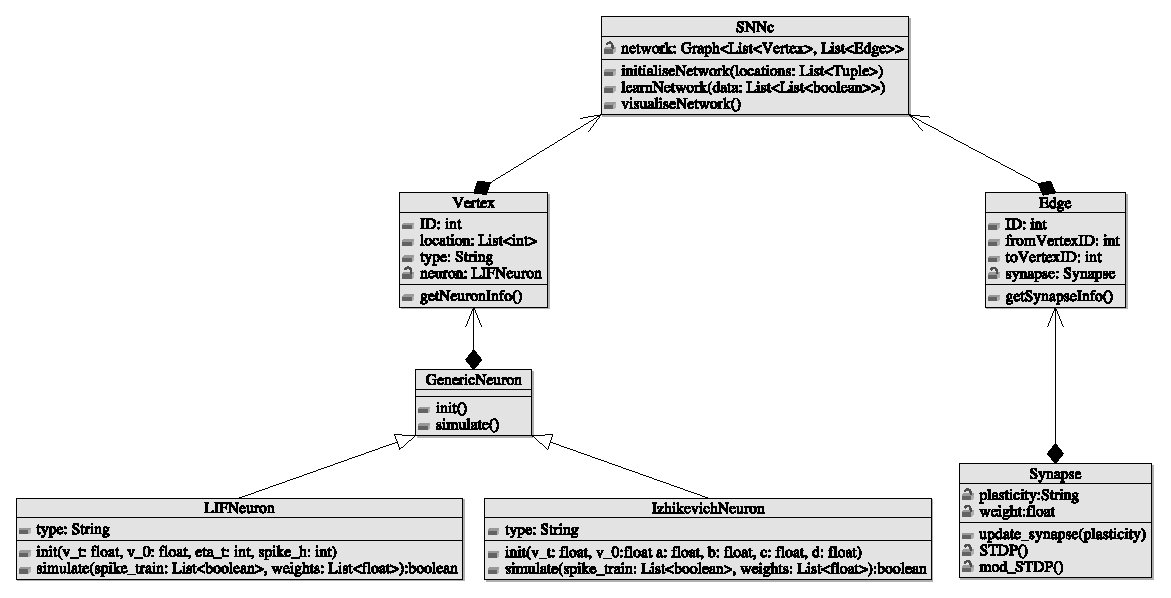
\includegraphics[width=0.8\linewidth]{fig/largesnn/class_diagram.eps}
	\caption{UML Class diagram of the template based object-oriented architecture of the SNNc. This architecture should be considered an example architecture for incorporating modularity. A python implementation of the SNNc following this architecture is presented in Appendix \ref{chap:app_SNNc_unsupervised}.}
	\label{fig:class_diagram}
\end{sidewaysfigure}

\section{Summary and Conclusion}
In this Chapter, the discussions have primarily revolved around the implementation aspects of the SNNc. This Chapter began by contemplating the discrepancy between a biological brain and a computer. The discrepancies formed the basis of the challenges that arises in developing human brain-like computation algorithms in computers. Then, there was a presentation of an in-depth formalisation, discussion and analysis of the several components of the SNNc architecture and unsupervised learning algorithms in NeuCube. This discussion paves the pathway for analysing the data structure representations of the SNNc network with respect to scalability and heterogeneity. During this discussion, it was shown how the network representation plays a decisive role in large scale implementations, especially balancing the storage and execution time. The importance of modularity and heterogeneity in SNNc was further discussed as well as a proposal put forward for a hierarchical template pattern-based software architecture for realising such a goal.


\pagebreak
\section{Contributions and Publications}
\begin{tcolorbox}[colback=black!5,colframe=black!40!black,title=Contributions]
	\itshape
	\begin{enumerate}
		\item There were qualitative comparisons of the contrasting characteristics of a biological brain and a computer.
		\item In-depth descriptions about the SNNc layer of the NeuCube architecture were made. This included SNNc network initialisation, simulation and learning with formalisation of the unsupervised learning algorithm.
		\item An analyses of the SNNc network storage architecture and data structure was presented in the light of large scale simulation of the SNNc.
		\item A template pattern based software design architecture of SNNc to incorporate modularity and heterogeneity in the SNNc was proposed and implemented.   
	\end{enumerate}

\end{tcolorbox}

\begin{tcolorbox}[colback=black!5,colframe=black!40!black,title=Publications]
	\begin{enumerate}
		\item Abbott, A., \textbf{Sengupta, N.}, \& Kasabov, N. (2016, July). Which method to use for optimal structure and function representation of large spiking neural networks: A case study on the NeuCube architecture. In Neural Networks (IJCNN), 2016 International Joint Conference on (pp. 1367-1372). IEEE.
	\end{enumerate}
\end{tcolorbox}




\chapter{A Novel \emph{a priori} Knowledge Driven Temporal Encoding Framework for Compressing and Recognising Pattern on Temporal Data }
\label{chap:encoding}

\section{Introduction}

%It is without a doubt that in the era of `smart' everything, availability and utility of massive volumes of digital data plays a substantial role. Historically, data was used as a part of business and gathered to serve specific needs. For example, retailers recorded sales for accounting, manufacturers recorded raw materials for quality management the number of mouse clicks on advertising banners was collected for calculating advertisement revenue and so on. But as the demand for big data analytics emerged, data no longer serves only its initial purpose. Organisations able to access huge amounts of data possess a valuable asset that when combined with the ability to analyse it, has given rise to a whole new industry.

%According to IBM \cite{data2015four}, the big data ecosystem, even though related to its earlier versions of data analytics, differs from and is characterised by the following properties:
%\begin{itemize}
%	\item Volume: This is the main characteristic of 'big data'. It is predicted that the sheer volume of data will surpass 40 zetabytes by 2020, which is a $300$ times increase from 2005 \cite{data2015four}. In the past decade, organisations have begun to store and digitise multitude of data which is leading to the exponential rise of the digital data volume. Big data technologies aims to handle such rapidly growing volume of data and deliver actionable insights from analysing such data within a time frame.   
	
%	\item Variety: This is another important property of 'big data'. Variety is associated with the availability of diverse data sources with varying properties. Variety is one the most interesting developments in technology as more and more information is digitised. Earlier due to the structured nature of data, things fit neatly in relational databases. However, with variety in the data, the lack of structure in multi-source data has a major impact on the development of big data technologies. Structured data is augmented by unstructured data, which is where things like twitter feeds, audio files, MRI images, web pages, web logs are put, anything that can be captured and stored but does not have a meta model that neatly defines it.  
	
%	\item Velocity: Velocity relates to the frequency with which a data source streams the data and also the frequency with which analytics in 'big data' environment should be able to process the data. With the rise of IoT devices and technology there has been a substantial growth in streaming data. For example, New York stock exchange streams $\approx 1$ TB of trade information every session \cite{data2015four}, modern cars have more than $100$ sensors that continuously streams high velocity data. As a result, the 'big data' technologies focus on high speed analytics that allows for actionable insight delivery.  
%\end{itemize}

Traditionally, data analytics, especially, predictive analytics and machine learning have focused on computer intensive approaches that are intended to be applied directly to the raw data present in the continuous space \citep{bishop2006pattern}. These methods aim to take advantage of the flexibility entailed by continuous mathematics (uncountable sets) to build complex learning theories that can perform pattern recognition in data. However, with the rise of big data, the machine learning technologies are dealing with new challenges with respect to real time processing of massive volumes of data. Although the machine learning community has continuously striven to learn from massive volumes of data, the development has been grounded on the assumption that the computation fits into the memory seamlessly. In contrast, the current data size has grown to such a scale that the data are becoming harder to store. 

\section{Data Compression and Inspirations from Neural Coding}
In this Chapter, the focus will be on the inspirations from the human brain that allows us to see the problem of data processing and predictive analytics problem under the big data environment from an alternate perspective. It can be observed that the continuous incoming stimuli in various forms and frequencies processed by the human brain can indeed be characterised by the properties of big data, \emph{i.e.}, volume, variety and velocity. The human brain is considered to be the most resourceful and efficient system which can recognise distinct patterns in the streaming continuous stimuli (volume) captured by multiple sensory organs (variety) in millisecond resolution (velocity). It is also observed that human brain cells, when presented with external stimuli, propagates the signal economically, over long distances using electrical impulses or spikes via the synaptic action potentials. Hence, it is imperative that there exists an efficient system, which converts the massive volume of continuous signal to discrete events or spikes. In neurobiology, the process of such analog to digital signal transformation is known as neural encoding \citep{brown2004multiple}. It is intriguing that the process of neural encoding not only converts the big streaming continuous data space into a compressed space of spikes, but the brain cells also recognise patterns in such a compressed space. The biological organisation of the brain tends to create signals with a very specific class of distributions, and it is from the perspective of evolutionary understanding that these distributions are optimised for fast analysis. The most popular hypothesis states that the signal strengths are encoded by the mean firing rate, \emph{i.e.} stronger input signal produces larger volumes of neuronal firing on an average in the brain. A range of studies \citep{mainen1995reliability, maunsell1992visual} across multiple species in the sensory and motor-neuronal system supports the validity of the mean firing rate hypothesis. A major drawback of this theory, however, lies in the association of information density with spike density. Determining the spike density in millisecond resolution from a large volume of spikes leads to a level of computational inefficiency. As per an alternate theory on neural encoding, neurons carry information in the precise timing of the spikes. This is known as the temporal encoding or spike-time encoding. Numerous research \citep{gollisch2008rapid,hallock2006temporal} has shown the presence of temporal encoding in different parts of the human brain. Temporal encoding supports the efficient representation of information that is required for very fast processing (in millisecond scale) of the stimulus presented to the human brain. As opposed to the rate coding scheme, high fluctuations in mean firing rate, also known as inter-spike interval (ISI) probability distribution is considered to be informative rather than noise in this scheme. The temporal spike-time representation of the data acts as a lossy compression of information. Most forms of learning, though, could be seen as forms of data compression. In fact, one can, in terms of pattern recognition, only learn something from data when there is redundancy in the data. In many data analysis tasks, the data is preprocessed or recoded in a way that could be seen as a form of data compression. If such preprocessing does not destroy the patterns of interest, it results in a comparative performance of the learning algorithms. The motivation of the temporal encoding, thus, in this context is to reduce large volumes of data into a compressed state with minimal loss and the maximal presence of discriminable information. Examples of data sources where such encoding is useful are high-frequency streaming data, such as the pulsar data in radio astronomy, and seismic activity data. 

\subsection{Information Theory and Data Compression}

From the viewpoint of computational theory, the data encoding problem relates to the concepts of information theory. In the seminal work on information theory, \citet{shannon2001mathematical} proposed a mathematically complete theory to quantify transmission of information in a communication channel. A conclusive finding that the amount of information in any object can be estimated as the description length of the object continues to set the stage for the development of communications and data processing. Shannon's information theory is built on a presupposition that the computable information in an object is the characteristic of a random source with known probability distribution of which the object is a part. To realise this idea, Shannon derived the `entropy' from the first principle of the theory, which is the measure of average information emitted by an object when observed. It can be described as the functional mapping of the random variable to a real number. \citet{kolmogorov1965three}, later proposed an alternate and more generalisable notion of information measurement known as algorithmic information theory. Contrary to Shannon's theory, Kolmogorov's theory of complexity \citep{kolmogorov1965three, chaitin1966length} considers information as the property of an object in isolation, irrespective of the way the object came into existence \citep{grunwald2004shannon}. It describes information as the minimum number of bits from which a message or a file can effectively be reconstructed, \emph{i.e.} the minimum number of bits suffice to store a reproducible file. A computational neuron responsible for emitting spikes from sensory data can be regarded as a logical transmission medium responsible for broadcasting continuous information received from the data source. The two neural coding hypotheses hence can be seen and described in the light of information theory. It can be observed that the rate coding scheme adheres to Shannon's interpretation of encoding. The inherent assumption of the presence of a random source with a known probability distribution in Shannon's theory is much apposite to the mean firing rate as it relates to the frequency of spikes over time. However, the interest in efficient compression of a large volume of data by a sequence of spike-timings and using it for the purpose of pattern recognition is much more in line with Kolmogorov's notion of object representation by minimal description length using computer programs. 

\section{Literature Review on Analog to Digital Data Transformation Algorithms}
A significant amount of research has focused on using the biological realism of the SNN for information processing applications akin to traditional neural networks \citep{maass1997networks}. Under the broad umbrella of SNN, the area of data encoding has been relatively unexplored compared to neuronal dynamics, network learning behaviours and so on. Human Information Processing Research Laboratory's (Advanced Telecommunication Research Institute) artificial brain (Cellular Automata Machine Brain) project \citep{de1994artificial} used data encoding as a part of its large-scale brain-like neural architecture. Hardware accelerated implementation of spike encoding for image and video processing was performed by \citet{iakymchuk2014hardware}. The literature on the application of spike encoding on the information processing task in data science is restricted to a few algorithms, such as temporal-contrast (TC) \citep{kasabov2016evolving}, Hough spiker algorithm (HSA) \citep{hough1999spiker} and Bens spiker algorithm (BSA) \citep{schrauwen2003bsa}. HSA and BSA algorithms are event-driven in nature and can be classified under the temporal encoding paradigm where the time of occurrence of an event (spike) is considered as a unit of information. The TC algorithm, also known as AER encoding, is inspired from the human visual cochlea. The TC algorithm uses a threshold-based method to detect signal contrasts or changes \citep{kasabov2016evolving}. A user-defined or auto-generated contrast threshold determines the spike events in the TC algorithm. The HSA and BSA algorithm, however, determine a spike event using a deconvolution operation between the observed signal and a predefined filter. The HSA method which is based on convolution function produces a biased converted signal where it always stays below the original waveform and this would yield an error. The BSA method on the other hand uses the Finite Impulse Response (FIR)
reconstruction filter. Even though BSA reduces the error in the HSA method and has less optimal threshold sensitivity, this method like HSA, needed a suitable filter for every type of input. Finding this filter automatically for each image would require a tremendous amount of work and time. There are some LIF neural network modelling approaches that for analog to digital transformation applied to computer vision \citep{van1998face}. These methods, however, require a large number of input neurons. 

\section{A General Framework of Spike-time Encoding and Compression for Temporal Data Sequences}
\label{sec:general}

The temporal encoding problem for pattern recognition can be formalised as a data compression problem. An encoder is hence defined as the map $\displaystyle E:\mathbb{R}^T\rightarrow\mathbf{t}^f$, where the encoder $\displaystyle E(\cdot)$ release spikes at firing times $\displaystyle \mathbf{t}^f:=\{t_1^f, t_2^f,\cdots t_n^f|t_i\in \mathbb{I}^+\}$. The temporal encoding algorithm primarily assumes that the discriminatory information is encoded by the sequence of discrete spike-timings rather than the magnitude and/or the spike density. As a consequence of this assumption, the temporal encoding aims at joint maximisation of information representation and minimisation of the spike density. Thus, it is in sharp contrast to the rate coding hypothesis. Next, the proposed \emph{a priori} knowledge driven generalised framework for temporal encoding will be presented. This framework will be further extended to formalise a temporal encoding algorithm for fMRI data.

\subsection{Formalisation of the \emph{a priori} Knowledge Driven Optimisation Problem for Data Encoding}
If one assumes a continuous source signal is represented by $ \mathbf{s}\in \mathbb{R}^T$ representing a vector of continuous values, an encoded data or a spike-train is represented by $\mathbf{b}\in \{0, 1\}^T$ as a fixed-length binary sequence. This formalisation is slightly modified from the variable length sequence formalisation of spike-timings $\{t_1^f, t_2^f,\cdots t_n^f|t_i\in \mathbb{I}^+\}$ defined earlier without any loss of generality. For example, a historical spike sequence $[01001011]$ can be rewritten as a sequence of spike-time indices $t^f :=\{1, 4, 6, 7\}$. $T$ denotes the length of the temporal signal to be encoded into spikes. The \emph{a priori} knowledge driven optimisation based encoding framework is built on the premise that 
\begin{itemize}
	\item The universal data encoder is non-existent.
	\item \emph{a priori} knowledge about the data generation process or in other words, prior knowledge of the properties of the data generation source can be injected into a predictive system that can generate a predicted signal $\mathbf{\hat{s}}$. 
\end{itemize}
For example, the fMRI data generation process behaves like a linear time invariant system, where a spike in the brain cell gives rise to a signal mimicking the gamma distribution function \citep{ashby2011statistical}, whereas the process of EEG data generation can be modelled as a phase varying mixture model of sinusoidal waves or multi-source Gaussian noise model \citep{nunezm2016eeg}. The notion of knowledge injection is further elaborated in Section \ref{sec:fmri} using fMRI as an example. If it is possible to formalise a decompression function $\mathbf{\hat{s}}$ from the spike sequence $\mathbf{b}$, the optimal encoding of data can be formulated as an optimisation problem that minimises the discrepancy between the predicted and the original signal. One way of realising such a discrepancy is by minimising the root mean squared error (RMSE) of decompression between the observed signal $s$ and the predicted signal $\mathbf{\hat{s}}:=f(\mathbf{b}, \mathbf{\Theta})$, $\mathbf{\Theta}$ being the set of additional parameters required along with $\mathbf{b}$ to describe the prediction function. The optimisation problem can be formulated as:
\begin{equation}
\begin{matrix}
\displaystyle \min_{\mathbf{b},\mathbf{\Theta}} &  \displaystyle \sqrt{\frac{\sum_t(s_t-\hat{s}(b_t,\mathbf{\Theta}))^2}{t}} \\
\textrm{s.t.} & \displaystyle b_t:=\mathbb{I}^+ \\
& \displaystyle 0\leq b_t\leq 1\\ 
& \displaystyle \sum_t b_t\leq \alpha  \\
& \displaystyle \boldsymbol{\beta}\leq \boldsymbol{\Theta} < \boldsymbol{\gamma} \\ 
\end{matrix}
\label{eq:opt}
\end{equation}

The above optimiser solves for the RMSE, subject to the following constraints:
\begin{enumerate}
	\item Binary constraints for spikes: The binary constraint for the spikes are implemented by forcing $B_t$ to be an integer and within a range of $[0, 1]$.
	\item Constraint on the number of spikes: The $\sum_t B_t\leq \alpha$ constraint enforces the maximum number of spikes to be limited to $a$. This constraint is of major importance from a biological plausibility perspective. Since the encoding scheme discussed here, aims to mimic the temporal coding behaviour of the human brain, it is always preferable to encode maximal information with the minimal number of spike.  
	\item Bounds can be set on the other parameters $\Theta$ to be optimised as part of the prediction model $f(\mathbf{B, \Theta})$.
\end{enumerate}

\subsubsection{Mixed Integer Optimisation and Genetic Algorithms}
The aforementioned optimisation problem is one related to mixed-integer programming optimisation. A mixed integer programming problem is an optimisation problem, linear or nonlinear, with or without constraints, in which some or all decision variables are restricted to have integer values. Such problems frequently arise in various application fields such as process industry, finance, engineering design, management science and others. 

Several classical computational techniques (such as, branch and bound technique, cutting planes technique, and outer approximation technique), which are reasonably efficient, have been proposed in the literature for solving mixed integer programming problems \citep{cooper1981survey, floudas1995nonlinear, grossmann2002review}. Over the last couple of decades, several stochastic algorithms have been developed and appropriately updated for problems related to mixed integer programming, such as simulated annealing, differential evolution and ant colony optimisation \citep{dorigo1996ant, babu2003differential, yiqing2007improved}. However, algorithms of this class generally harbour the capacity to provide near global optimal solutions, although the quality of the obtained solution is unstable and requires large amount of computation time.

Genetic algorithms (GA) are general purpose population based stochastic search methods inspired by Charles Darwin's principles of natural selection and genetics. \citet{holland1992adaptation} introduced the concept of GA, and it was used by \citet{kenneth1975analysis} to solve the optimisation problem. \citet{goldberg1989genetic} presents a detailed implementation of GA. To describe it in a simple manner, GA searches for sets of better solutions in the global search space. Potential solutions termed as chromosomes (individuals) are evolved iteratively over generations using a set of genetic operators such as selection, crossover and mutation. The quality of a solution or a population is measured by a fitness function, which is equivalent to a loss function in the field of machine learning and objective function in optimisation. The fitness function is responsible for evaluating how `fit' a chromosome is for reproduction. The selection operator chooses the best `fit' chromosomes for reproduction. In the reproduction process, new chromosomes are created by crossover and mutation operations. The Crossover operator blends the genetic information between chromosomes to explore the search space, whereas the mutation operator is used to maintain adequate diversity in the population of chromosomes to avoid premature convergence. The way the variables are coded into the chromosome is clearly essential for GAs' efficiency. Real coded genetic algorithms (RCGAs), which use real numbers for encoding, have fast convergence towards optima as compared to binary and Gray coded GAs \citep{deb2001multi,}. Also, `RCGAs' overcome the difficulty of Hamming Cliff
as in binary coded GAs. In the case of integer and mixed integer programming problems, many applications of GAs are available in the literature, some of which use binary coded representation \citep{cheung1997coupling, luo2001hybrid,hua2006effective} and some use real coded representations \citep{li1996nonlinear, yokota1996genetic, maiti2006application}.

Integer programming with GA modifies the vanilla GA algorithm in several ways:
\begin{enumerate}
	\item It requires custom creation, crossover and mutation function in order to enforce the variables to be integers (see \citep{deep2009real} for detail).
	\item The genetic algorithm attempts to minimise a penalty function, not the fitness function. The penalty function includes a term for infeasibility. This penalty function is combined with binary tournament selection to select individuals for subsequent generations. The penalty function value of a member of a population is:
		\begin{itemize}
			\item If the member is feasible, the penalty function is the fitness function.
			\item If the member is infeasible, the penalty function is the maximum fitness function among feasible members of the population, plus a sum of the constraint violations of the (infeasible) point. For details of the penalty function, see \citep{deb2000efficient}.
		\end{itemize}
	\item GA  does not enforce linear constraints when there are integer constraints. Instead, it incorporates linear constraint violations into the penalty function.
\end{enumerate}

In the present implementation, the mixed integer genetic algorithm solver \citep{deb2000efficient,deep2009real} was used. The constraints in \equationname \ref{eq:opt} are imposed on the parameters of $\hat{s}$. The first and second constraints are used to reduce the search space of the possible values of $b_t$ to $\{0, 1\}$. The hyperparameter $\alpha$ is used to control the maximum number of spikes and hence the spike density in the optimal solution. The other sets of hyper-parameters $\{\boldsymbol{\beta}, \boldsymbol{\gamma}\}$ are used to control the upper and lower bounds of the model parameter $\boldsymbol{\Theta}$. 

The formulation above for the proposed framework for data encoding is generic, flexible and is driven by knowledge-injection from the data source. The knowledge-injection component allows the further inclusion of systematic noise as part of $\mathbf{\hat{s}}$, if present. Examples of the inclusion of noise models, such as acoustic noise as part of linear time invariant models of fMRI are treated in \citep{sierra2008acoustic, cho1997analysis}. The hypothesis is that a sufficiently good choice of $\mathbf{\hat{s}}(\mathbf{b}, \mathbf{\Theta})$ preserves, in some cases, enhances the discriminative property of the data in a greatly compressed space. It must also be noted that this formulation adheres to the concept of the non-existence of a universal compression algorithm for all the data sources. The general framework described above can be used to derive specific methods for encoding of special types of data for which \emph{a priori} knowledge is available. One such case is fMRI data based on blood-oxygen level dependent response (BOLD). This is further introduced and illustrated in Section \ref{sec:fmri}. 

\section{GAGamma: A Spike-time Encoding and Compression Method for fMRI Data}
\label{sec:fmri}

This Section will formalise a sample prediction model $f(\mathbf{B, \Theta})$ for functional Magnetic Resonance Imaging (fMRI) data, and will present experimental results and evaluation of data encoding by solving \equationname \ref{eq:opt}.

\subsection{fMRI As a Linear Time Invariant System}

Functional magnetic resonance imaging (fMRI) is a form of magnetic resonance imaging that takes advantage of magnetic susceptibility artefacts caused by the deoxygenated haemoglobin in the brain. Magnetic susceptibility measures the magnetic properties of the interaction between a tissue or other substance and the in-scanner magnetic field strength. Magnetically susceptible materials distort the homogeneity of a magnetic field: materials with negative magnetic susceptibility are known as diamagnetic, and those with positive magnetic susceptibility are referred to as paramagnetic. Introduction of a paramagnetic substance such as deoxyhaemoglobin into the scanner magnetic field causes variability in field strength, spin dephasing, geometric distortion and loss of signal; fMRI exploits this property by measuring changes in the relative ratio of oxygenated (diamagnetic) to deoxygenated (paramagnetic) haemoglobin in the blood.

Functional Magnetic Resonance Imaging (fMRI) is most commonly acquired using Blood Oxygen Level Dependent (BOLD) response. The BOLD response is measured by the changes in deoxyhaemoglobin at time $t$, and is caused by neural activation in the brain. The neural activations are caused by some sequence of events driven by the task performed by the subject \citep{friston1995analysis}. The BOLD response is mathematically described as a time invariant system, \emph{i.e.} a system whose output does not depend explicitly on time. Under the appropriate experimental protocol, BOLD response also pertain to the superposition principle and henceforth can be designed as a linear time invariant (LTI) \citep{vazquez1998nonlinear}. According to \citet{chen1995linear}, a LTI system is said to be completely characterised by convolution integral functions. The fMRI BOLD is described by the convolution of the spikes $\mathbf{b}$ and the haemodynamic response function (HRF), $h(\mathbf{\Theta})$. This operation is characterised by \equationnames \ref{eq:conv1} and \ref{eq:conv2}. 

\begin{equation}
\label{eq:conv1}
\displaystyle \mathbf{\hat{s}}:=\int_0^t \mathbf{b}(\tau)h(t-\tau)d\tau
\end{equation}

\begin{equation}
\label{eq:conv2}
\displaystyle \mathbf{\hat{s}}(\mathbf{b}, \mathbf{\Theta}):=\mathbf{b}\ast h(\mathbf{\Theta})
\end{equation}

\begin{equation}
\label{eq:hrf}
h(\theta_1, \theta_2):=\frac{1}{\theta_2^{\theta_1}\mathcal{T}(\theta_1)}t^{\theta_1-1}e^{-\frac{t}{\theta_2}}
\end{equation}
\subsection{GAGamma Optimisation Problem for fMRI}
Numerous models for HRF have been proposed in the literature \citep{boynton1996linear,friston1998nonlinear,glover1999deconvolution}. The majority of mathematical models for the canonical HRF are found to be some variant of the gamma function. In all the experiments performed here, the gamma distribution function has been used as the HRF model (\equationname \ref{eq:hrf}). This function is characterised by the parameter set $\displaystyle \mathbf{\Theta}:=\{\theta_1, \theta_2\}$, where $\theta_1\in \mathbb{R^+}$ and $\theta_2\in \mathbb{R^+}$ controls the shape and the scale of the gamma function respectively. By substituting \equationnames \ref{eq:conv2} and \ref{eq:hrf} in \equationname \ref{eq:opt}, the encoding problem can be reduced to solving \equationname \ref{eq:gagamma} and is referred to as GAGamma encoding algorithm hereafter.

\begin{equation}
\begin{matrix}
\displaystyle \min_{\mathbf{b},\theta_1, \theta_2} &  \displaystyle \sqrt{\frac{\sum_t(s_t-\hat{s}(b_t,\theta_1, \theta_2))^2}{t}} \\
\textrm{s.t.} & \displaystyle b_t:=\mathbb{I}^+ \\
& \displaystyle 0\leq b_t\leq 1\\ 
& \displaystyle \sum_t b_t\leq \alpha  \\
& \displaystyle \beta_1\leq \theta_1\leq \gamma_1 \\ 
& \displaystyle \beta_2\leq \theta_2\leq \gamma_2 \\

\textrm{where} & \displaystyle \hat{s}_t(b_t,\theta_1,\theta_2):=b_t\ast \frac{1}{\theta_2^{\theta_1}\mathcal{T}(\theta_1)}t^{\theta_1-1}e^{-\frac{t}{\theta_2}}
\end{matrix}
\label{eq:gagamma}
\end{equation}

\subsection{Distinction of GAGamma from HSA and BSA}

At this point, it is imperative to make the distinction between the GAGamma and the existing HSA and BSA algorithms. Apart from exhibiting similarities in convolution framework, HSA and BSA also resemble GAGamma as methods of stimulus estimation using FIR. Nevertheless, the data encoding approach in HSA and BSA use a deconvolution (of \equationname \ref{eq:conv1}) approach contrary to the optimisation approach in GAGamma. The knowledge-injection component of GAGamma, as part of formalisation of $\mathbf{\hat{s}}$ and the optimisation approach, has two distinct benefits over the deconvolution-based methods: 
\begin{itemize}
	\item A generic Gamma function has been used as the knowledge-injection component to $\mathbf{\hat{s}}$ in GAGamma, which is driven by the existing knowledge about the fMRI data as opposed to the generic sinusoidal function used as the FIR in BSA. It is also argued that this formulation allows the inclusion of additional knowledge about the data source (such as systematic noise) if present, providing greater flexibility in the formulation of the encoding algorithm.
	
	\item The optimisation problem formulation in GAGamma jointly optimises for the parameter set $\mathbf{\Theta}$ and $\mathbf{b}$. This formulation thus includes the parameter set $\mathbf{\Theta}$ of the prediction model $\mathbf{\hat{s}}$ and the spike sequence $\mathbf{b}$ for each individual voxel or feature. In HSA and BSA, the equivalent filter parameters are predetermined for the whole set of voxels and are not learned from the data.
	
	\item The constraint $\everymath{\displaystyle} \sum_t b_t\leq \alpha$ in GAGamma ensures the flexibility in choosing the desired spike density, hence the ability to control the compression and quality of signal reconstruction. The BSA or HSA algorithm, on the contrary, accommodates no such control in the encoding framework.        
\end{itemize}

\section{Experiments and Evaluation}
\subsection{Description of Dataset}
The experiments described in this Chapter were performed on the publicly available benchmark Starplus fMRI dataset \citep{mitchell2001starplus} collected by The Centre for Cognitive Brain Imaging, Carnegie Mellon University. The Starplus experiment was conducted on a set of $7$ subjects. Each subject had undergone multiple trials of exactly the same cognitive experiment. At every trial lasting for $27$ seconds, a set of stimuli were presented to a subject in the following order:
\begin{enumerate}
	\item The first stimulus (picture or sentence) was presented at the beginning for 4 seconds.
	\item A blank screen was presented during the interval of $5-8$ seconds.
	\item The second stimulus (sentence or picture) was presented during the interval of $9-12$ seconds.
	\item A rest period of $15$ seconds was added after the presentation of the second stimulus.
\end{enumerate}
While the subject performed the cognitive tasks, fMRI images from specific regions of interest (ROI) of the brain were collected at every $500$ms interval. The preprocessed fMRI dataset has been used in a number of pattern recognition studies \citep{mitchell2003classifying, mitchell2008predicting, shinkareva2008using}. In this study, this benchmark dataset was chosen to build pattern recognition systems that can predict and discriminate between the binary cognitive states of a subject `seeing a picture' and `reading a sentence'. Two subjects were chosen (id: 04847 and 07510) randomly and two spatial ROIs; Calcarine Sulcus (`CALC') and Left Intra-Parietal Sulcus (`LIPL') were used for the experiments. The choice of the ROI is based on previous work \citep{do2014robust} that found these ROIs to be amongst the most discriminatory in the raw continuous data space. The dataset for each subject is composed of $40$ samples (trials) of each class, and each sample is made up of $452$ and $483$ voxels in subject 04847 and 07510 respectively. Each cognitive task lasted for a total of $8$ seconds emitting $16$ fMRI images for each class within a trial.

\subsection{Evaluation Metrics}

Three metrics have been used to evaluate and compare the performance of the encoding techniques and the traditional `no-encoding' (raw data) approach. The evaluation criteria and the baseline encoding techniques are elaborated below:

\subsubsection{Bit Compression Ratio} 
The Bit Compression Ratio (BCR) is defined as the ratio between the average number of bits required to store an encoded dataset and the number of bits required to store a raw dataset, respectively. BCR is directly associated with the relative description lengths (DL) and data type of the datasets. The DL of a dataset is described by the length of the dataset represented by the number of values in the dataset. If one assumes a dataset intended for pattern recognition is represented by $D_{raw}:=\{x_1, x_2, \cdots x_n| type(x_i)=\mathbb{R}\}$ which is transformed by an encoding algorithm to $D_{encoded}:=\{y_1, y_2, \cdots y_m| type(y_j)=\mathbb{I}^+\}$, where $m$ and $n$ are the DL of the raw and the encoded data respectively. The BCR is then estimated as:
\begin{equation}
	BCR:=\frac{m\times sizeof(\mathbb{I}^+)}{n\times sizeof(\mathbb{R})}
\label{eq:compression}
\end{equation}  
The notion of BCR (\equationname \ref{eq:compression}) can be analysed from the viewpoint of the Kolmogorov complexity. As described earlier, Kolmogorov's descriptional complexity aims at a simpler object representation and simplicity is measured by the DL of the object. Here, the object being a pattern recognition dataset, the objective is to achieve simpler representation of the dataset by performing the encoding operation. This is achieved by minimising the numerator $m\times sizeof(\mathbb{I}^+)$. A compression is said to be achieved, if $0<BCR<1$ is satisfied. It is also quite evident from \equationname \ref{eq:compression} that the data type of the objects present in the dataset contributes significantly to the BCR metric. In this case, the encoded data being represented by positive integers (spike-timings) as opposed to the floating-point numbers in the raw data, already contribute significantly to BCR. Additionally, the temporal encoding algorithms aspire to minimise the DL of the object ($m<<n$), thus achieving a lower BCR.            
	
\subsubsection{Decoding Error} The decoding error metric is the measure of the decompression reliability, \emph{i.e.} the ability to recover the original signal from the compressed spike-timings reliably. RMSE of signal reconstruction between the original signal $s$, and the predicted signal $\hat{s}$ has been used as a measure of decompression reliability in this study. The RMSE is given by:
\begin{equation}
	\displaystyle RMSE:= \sqrt{\frac{\sum_t(s-\hat{s}(b_t,\Theta))^2}{t}}
\end{equation}
A low RMSE of the signal reconstruction indicates higher preservation of the original data in the spike-timings. However, low RMSE is not necessarily indicative of a better encoding for pattern recognition. For example, an encoder producing better reconstruction error for noisy data may indicate inefficient noise filtering. It must also be noted that the prediction models are built on the spike-time data and have no knowledge of the mapping $\mathbf{s}\rightarrow \mathbf{b}$ being performed beforehand. Hence, although this metric plays an important role in evaluating the robustness of the encoding algorithm with respect to the reconstruction of the raw data, the effect on the quality of pattern recognition performance is unaffected.
	
\subsubsection{Classification Performance} From the pattern recognition viewpoint, due to the balanced nature of the dataset, the classification accuracy is the most important and relevant measure of success and this has been used as a measure of classification performance. The mean accuracy is estimated from thirty independent runs of 50/50 train/test split of the binary classification data described previously. 

As the data that was encoded was intended to be used for pattern recognition problems, conservation and possible enhancement of the discriminatory information in the spike-timings is as crucial as efficient compression of the data. This is a distinctly different approach from the existing ones in pattern recognition. In the traditional pattern recognition approach, the volume of the data plays a crucial role in the performance of the pattern recognition algorithms to produce accurate predictions. In the temporal encoding approach, by keeping both compressibility and classification performance as the criteria of evaluation, the aim is to benefit from the efficient representation of information in the data along with the classification performance. It is, thus, important to have a balance between compression and conservation of discriminatory information in the encoded data. 

\subsection{Design of Experiments}
\begin{figure}
	\centering
	\includegraphics[width=\linewidth]{fig/encoding/flowchart.png}
	\caption{Flowchart depicting the evaluation criteria and experimental protocol used in this research.}
	\label{fig:flowchart}
\end{figure}

\figurename \ref{fig:flowchart} shows a flowchart of the experimental design used in this Chapter. The experimental protocol begins with the raw temporal data $\mathbf{s}$. At the first step, the encoding operation is performed on $\mathbf{s}$ to generate the encoded spike-time data $\mathbf{b}$. In the second step, a K-NN based prediction model is learned using a fraction of $\mathbf{b}$. The rest of $\mathbf{b}$ is used to test the performance of the model emitting the prediction performance. The next evaluation criteria relate to the compressibility of the encoding algorithms. To evaluate the compressibility, BCR is calculated by comparing $\mathbf{b}$ and $\mathbf{s}$. Finally, the lossiness of the encoding operation is evaluated by comparing predicted signal $\hat{s}$ produced by the decoding algorithm (corresponding to the encoding algorithm) and the ground truth $s$ to emit the decoding error.   

\subsubsection{K-Nearest Neighbour (K-NN) Algorithm with Custom Distance Function}
\label{parag:knn_custom}
As discussed earlier, the non-parametric K-NN algorithm for building the classification model from the data is used. The class label prediction of a new sample (in this case a spike-train) in K-NN is a majority vote between the neighbours of the new sample, where the sample is assigned to the class label most common among its K nearest neighbours. To evaluate the neighbourhood of a sample, it is hence necessary to calculate pairwise distances between the sample to be predicted and the training samples. As the key interest is in learning about a K-NN model for both raw (in continuous space) and spike-time (discrete space) data, there have been two different distance functions used: raw and encoded data. For the raw data in the continuous space, the standard Euclidean distance or the $L^2$ norm as the distance function was used. On the other hand, for the spike-time dataset, the spike asynchronicity based distance function was used, and is described below:

\paragraph{Spike asynchronicity based distance function:} Here, I propose a distance function that can capture the relative distance between a pair of the spike-train samples. Since the concern is with using spike-timings as a carrier of information, a useful way to capture similarity between a pair of spike-train samples is to record if the two samples have spiked at the same time instances. Therefore, mean absolute asynchronicity has been used as the distance function. The mean absolute asynchronicity based distance function between two spike-train samples $\displaystyle \mathbf{b_1}\in \{0, 1\}^{T\times M}$ and $\displaystyle \mathbf{b_2}\in \{0, 1\}^{T\times M}$ is formalised as the mean pairwise Hamming distance between all feature-wise pairs $\mathbf{b_1^{m}}$ and $\mathbf{b_2^{m}}$, where $M$ is the feature count. As the spike-time data lies in the binary space, the mean pairwise Hamming distance is equivalent to the mean XOR distance between the pairs of spike sequences. 

\subsection{Baseline Encoding Algorithms}    

In this study, three different encoding methods have been compared and evaluated. It must be noted that for each encoding or compression algorithm, there is also a decoding algorithm which decompresses the spike-trains into the reconstructed signal $\mathbf{\hat{s}}$.   
\begin{algorithm}
	\begin{algorithmic}[1]
		\STATE input: $s, filter, threshold_{BSA}$
		\STATE output: $b$
		\STATE $b\Leftarrow 0$
		\STATE $L=length(s)$
		\STATE $F=length(filter)$
		\FOR{$t=1:(L-F+1)$}
			\STATE $e_1\leftarrow 0$
			\STATE $e_2\leftarrow 0$
			\FOR{$k=1:F$}
			    \STATE $e_1 \pluseq |s(t+k)-filter(k)|$
			    \STATE $e_2 \pluseq |s(t+k-1)|$      
			\ENDFOR
			\IF{$e_1\leq (e_2-threshold_{BSA})$}
			    \STATE $b(t)\leftarrow 1$
			    \FOR{$k=1:F$}
			        \STATE $s(i+j-1)\minuseq filter(k)$
			    \ENDFOR
			\ENDIF
		\ENDFOR
		\caption{BSA encoding algorithm}
		\label{alg:bsa-enc}
	\end{algorithmic}
\end{algorithm}

\begin{algorithm}
	\begin{algorithmic}[1]
		\STATE input: $b, filter$
		\STATE output: $\hat{s}$
		\STATE $L=length(b)$
		\STATE $F=length(filter)$
		\FOR{t=1:L-F+1}
		    \IF{$b(t)==1$}
		        \FOR{$k=1:F$}
		            \STATE $\hat{s}(t+k-1)\pluseq filter(k)$
		        \ENDFOR
		    \ENDIF
		\ENDFOR
		\caption{BSA decoding algorithm}
		\label{alg:bsa-dec}
	\end{algorithmic}
\end{algorithm}


\begin{itemize}
	\item GAGamma: The GAGamma encoding method is outlined and described in Section \ref{sec:fmri}. The encoding and decoding principles are given by \equationnames \ref{eq:conv2} and \ref{eq:gagamma}.
	
	\item BSA: The BSA encoding and decoding algorithms \citep{schrauwen2003bsa} are formalised in \algorithmnames \ref{alg:bsa-enc} and \ref{alg:bsa-dec}, respectively. The BSA encoding algorithm takes a filter function and a threshold value as input along with the signal $s$. The deconvolution approach of BSA begins with a FIR filter, and at every time instant $\tau$ calculates two error metrics: $\sum_{k=0}^{P}abs(s(k+\tau)-h(k))$ and $\sum_{k=0}^{P}abs(s(k+\tau)$, where $P$ is the number of filter taps. If the first error is less than the second error minus the threshold, then the BSA encoder fires a spike and subtracts the filter from the input \citep{schrauwen2003bsa}.  
	
	\item Temporal contrast: The temporal contrast algorithm captures the greater than average changes in the data as spikes. \algorithmnames \ref{alg:tc-enc} and \ref{alg:tc-dec} presents the temporal contrast encoding and decoding algorithms respectively. One major characteristic and deviation of temporal contrast algorithm from the temporal encoding framework is its ability to generate spikes with positive and negative polarity. Since the main interest is in the spike-timings, during the classification, the polarity of the spikes have been ignored. The algorithm takes the $factor\in \{0, 1\}$ parameter as input. This parameter controls the estimate of the $threshold_{TC}$ variable, which is responsible for determining the spike-timings. 
	
\end{itemize}
\begin{algorithm}
		\begin{algorithmic}[1]
			\STATE input: $s$, $factor$
			\STATE output:$b, threshold_{TC}$
			\STATE $L\leftarrow length(s)$
			\FOR {$t=1:L-1$}
			\STATE $diff\leftarrow |s(t+1)-s(t)|$
			\ENDFOR
			\STATE $threshold_{TC}\leftarrow mean(diff)+factor\cdot std(diff)$
			\STATE $diff\Leftarrow [0,diff]$
			\FOR{$t=1:L$}
			\IF{$diff(t)>threshold_{TC}$}
			\STATE $b(t)\leftarrow 1$
			\ELSIF{$diff(t)<-threshold_{TC}$}
			\STATE $b(t)\leftarrow -1$
			\ELSE
			\STATE $b(t)\leftarrow 0$
			\ENDIF
			\ENDFOR
			\caption{Temporal contrast encoding algorithm}
			\label{alg:tc-enc}
		\end{algorithmic}
	\end{algorithm}

	\begin{algorithm}
		\begin{algorithmic}[1]
				\STATE input: $b, threshold_{TC}$
				\STATE output: $\hat{s}$
				\STATE $\hat{s}\leftarrow 0$
				\STATE $L\leftarrow length(b)$
				\FOR {$t=2:L$}
				\IF{$\hat{s}(t)>0$}
				\STATE $\hat{s}(t)\leftarrow \hat{s}(t-1)+threshold_{TC}$
				\ELSIF{$\hat{s}(t)<0$}
				\STATE $\hat{s}(t)\leftarrow \hat{s}(t-1)-threshold_{TC}$
				\ELSE
				\STATE $\hat{s}(t)\leftarrow \hat{s}(t-1)$
				\ENDIF
				\ENDFOR
				\caption{Temporal contrast decoding algorithm}
				\label{alg:tc-dec}
		\end{algorithmic}
	\end{algorithm} 
\subsection{Results}

\begin{table}
	\centering
	\caption{Comparative evaluation of the data encoding algorithms applied to subject 04847 and 07510 in the Starplus fMRI dataset.}
	\label{tab:classification}
	\resizebox{\textwidth}{!}{%
		\begin{tabular}{@{}clcccc@{}}
			\toprule\toprule
			subject id & method & data type \footnotemark{} & BCR & decoding error & classification accuracy (K\footnotemark{}) \\ \midrule
			\multirow{5}{*}{04847} & GAGamma-16 & int & $0.15$ & $\mathbf{0.07}$ & $87.41\pm 4.80 (16)$  \\
			& GAGamma-3 & int & $\mathbf{0.04}$ & $0.29$ & $85.02 \pm 4.76 (11)$ \\
			& BSA & int & $0.08$ & $0.15$ & $84.5\pm 4.47 (3)$ \\
			& TC & int & $0.06$ & $0.23$ & $54.16\pm 5.47 (1)$ \\
			& No-encoding & decimal & $1$ & - & $\mathbf{89.55\pm 4.60} (1)$ \\\midrule
			\multirow{5}{*}{07510} & GAGamma-16 & int & $0.15$ & $\mathbf{0.06}$ & $76.00\pm 5.89 (8)$ \\
			& GAGamma-3 & int & $\mathbf{0.04}$ & $0.27$ & $\mathbf{81.16\pm 7.50} (2)$ \\
			& BSA & int & $\mathbf{0.04}$ & $0.15$ & $74.08\pm 6.71 (8)$ \\
			& TC & int & $0.05$ & $0.26$ & $52.75 \pm 5.84 (2)$ \\
			& No-encoding & decimal & $1$ & - & $79.11 \pm 3.99 (5)$ \\\midrule
			& Random & int & $0.11$ & - & $52.58\pm 4.79 (1)$ \\ \bottomrule\bottomrule
		\end{tabular}%
	}
\end{table}
For the comparative evaluation of the encoding methods with the classical `no-encoding' (raw data) method, identical experiments were performed for the subjects 04847 and 07510. For the GAGamma encoding, two sets of hyper-parameters have been used to demonstrate the tuning capability of the algorithm. In the GAGamma-16  method, the hyperparameter values $[\alpha=16, \beta=0, \gamma=10]$ (see \equationname \ref{eq:gagamma}) were used, and in the GAGamma-3 method, $[\alpha=3, \beta=0, \gamma=10]$ were used. The BSA encoding algorithm takes a finite impulse response $filter$ and a $threshold_{BSA}$ as input. In the current experiments, the low pass FIR filter of size $10$ and the $threshold_{BSA}=0.95$ have been used. These values are guided by the existing literature on the application of BSA on brain data \citep{nuntalid2011eeg}. For the temporal contrast encoding, the hyper-parameter $factor=0.6$ has been used. As a baseline, a randomly generated spike-train dataset has also been included. The random spike-time dataset was created using a Poisson's distribution function ($\lambda=0.6$). Varying the $\lambda$ parameter affects the BCR directly for random spike generation. It must be noted that the presented results are non-exhaustive in the hyperparameter space of different encoding methods. In the `no-encoding' method, the raw dataset was created by transforming each multi-dimensional time series (set of images) within a trial into a single static observation by concatenating the feature values across the $16$ time intervals similar to the approach employed by \citet{mitchell2003classifying}. 

\footnotetext[1]{An integer is assumed to take 8 bits and floating-point number 32 bits.}    
\footnotetext[2]{K: Number of nearest neighbours used in K-NN algorithm}


\subsubsection{Comparison Between `Encoding' and `No-encoding'} The advantages of performing encoding as opposed to using the raw data (`no-encoding') is well established in \tablename \ref{tab:classification}. This table shows the experiments replicated across subjects 04847 and 07510. For every subject, three temporal encoding methods were evaluated. They are the proposed GAGamma, BSA and the temporal contrast encoding. In the GAGamma-X method, $X$ corresponds to the value of the maximum number of allowed spikes, $\alpha$ (\equationname \ref{eq:gagamma}). The temporal encoding methods are compared against the raw data or the `no-encoding' method along with a random spike-train as a baseline. As discussed earlier, the encoding methods are evaluated using BCR, decoding error and classification accuracy as the measures of success. The decoding error metric is not applicable for the `random' and `no-encoding' method. This is because in `no-encoding' and `random' method, the raw data and a random spike generator were used, respectively, for pattern recognition and thus, encoding principles are not applied in these two cases. 
	
It is observed that the encoding operations could compress the data dramatically and thus attaining BCR values between $0.04$ and $0.15$ \emph{i.e.} an approximate compression of $6$ to $25$ times compared to the raw data. The most important metric of evaluation, the classification accuracy column in \tablename \ref{tab:classification}, shows that the GAGamma and BSA methods achieve comparable classification performances with respect to the `no-encoding' method, and hence can capture the discriminatory information in the spike-time data well. It should also be noted that for subject 07510, the GAGamma-3 method achieved a classification performance of $81.16\pm 7.50\%$ as opposed to the $79.11\pm 3.99\%$ by the raw data and thus outperforming the `no-encoding' method. This, it can be argued is due to the ability of the encoding algorithms to represent the information in the raw data into the spike-time and thus concisely present to the classifier.
	
\subsubsection{Comparison of the Temporal Encoding Algorithms} 

\begin{figure}
	\centering
	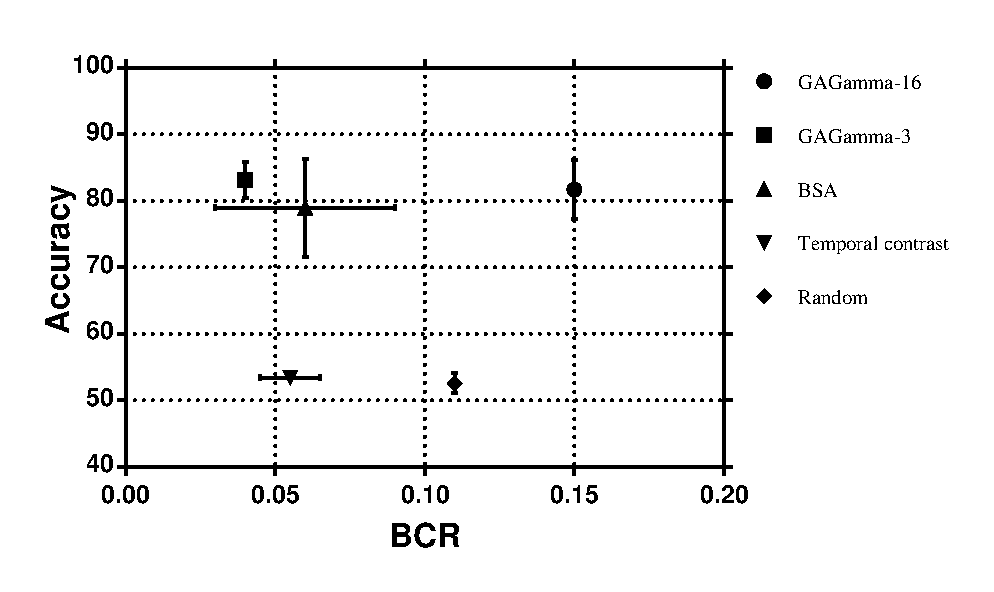
\includegraphics[width=\linewidth]{fig/encoding/encoding_comp_graph.eps}
	\caption{Plot illustrating the comparison of the quality of the encoding methods with respect to the mean classification accuracy and bit compression ratio across the two subjects. The horizontal and the vertical error bars represent the standard deviation of accuracy and BCR across experiments.}
	\label{fig:eval-chart}
\end{figure}


\figurename \ref{fig:eval-chart} graphically depicts the quality comparison of the different encoding techniques. The plot shows the mean BCR and the classification accuracy of the encoding techniques across the two subjects. The horizontal and vertical error bars are the standard deviations of the BCR and accuracy respectively. It can be initially observed that the GAGamma-16 and GAGamma-3 encodings show superior mean performance in the pattern recognition task compared to other methods. However, the aim is to simultaneously achieve high classification performance and a highly compressed information representation, and thus, the GAGamma-3 and BSA data points residing on the top left quadrant of the plot fare better overall in both respects. From the error bar representations, it can also be seen that the GAGamma method has a negligible deviation on BCR. This is due to the flexibility that the GAGamma method provides to control the spike density by the constraint $\everymath{\displaystyle} \sum_t b_t\leq \alpha$ (\equationname \ref{eq:gagamma}) without sacrificing much pattern recognition performance. This can be of significant importance, especially, for the storage and transmission of large volumes of streaming data within limited resources, where the encoding operation can precisely tune the compression rate and hence the storage. It is also recognised from the plot that the temporal contrast encoding method fares poorly in this experiment and is no better than a random spike generator.              

\begin{figure}
	\centering
	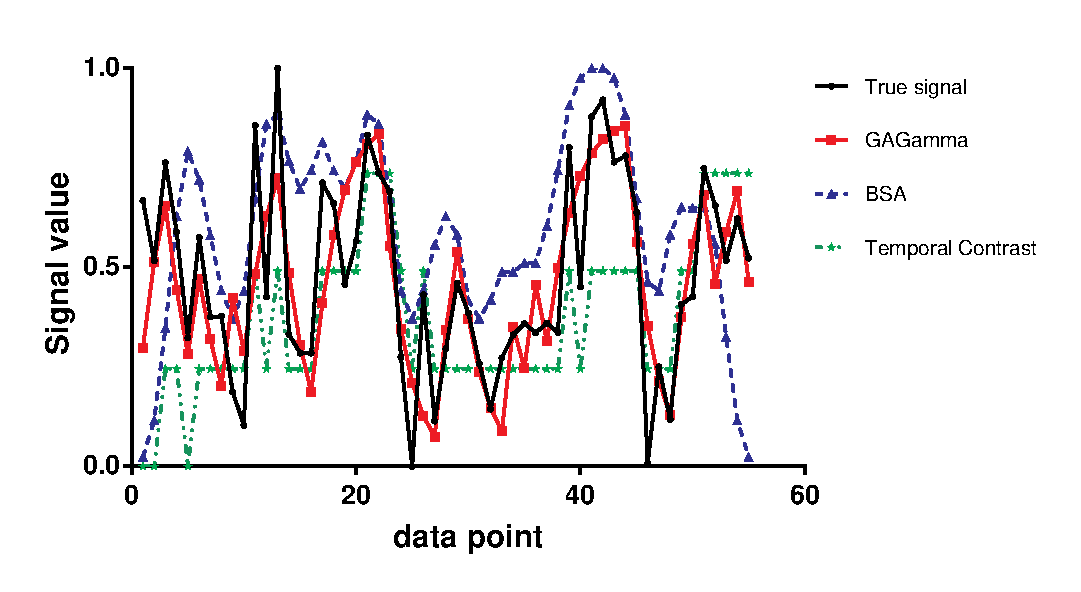
\includegraphics[scale=0.9]{fig/encoding/signal_recon.eps}
	\caption{Comparison of signal reconstruction ($\hat{s}$) from a spike sequence by GAGamma-16 decoding  algorithm (\equationname \ref{eq:conv2}), BSA decoding algorithm (\algorithmname \ref{alg:bsa-dec}) and Temporal contrast decoding algorithm (\algorithmname \ref{alg:tc-dec}). The true signal is randomly selected from subject 04847 ($10^{th}$ trial and $23^{rd}$ voxel).}
	\label{fig:recon}
\end{figure}


\begin{figure}
	\centering
	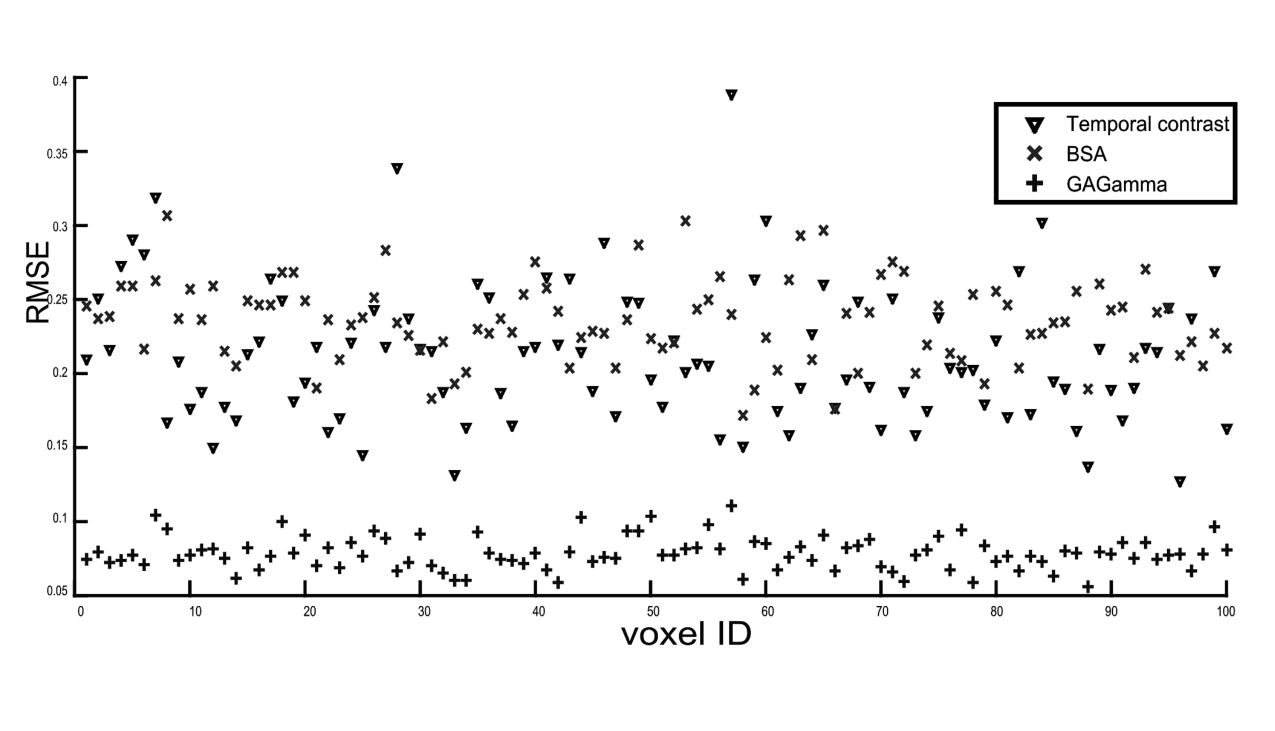
\includegraphics[width=\linewidth]{fig/encoding/recon.eps}
	\caption{Comparison of RMSE of reconstruction between GAGamma, BSA and Temporal Contrast across $100$ voxels of second trial in subject 04847.}
	\label{fig:RMSE}
\end{figure} 

\tablename \ref{tab:classification} also shows an inverse relationship between the BCR and the decoding error. This is because it requires significantly more effort to accurately represent the seasonal variations in the data using fewer spikes. However, if decoding robustness is of major importance, the GAGamma method can be tuned to maximise spike density and thus will have minimal loss in the signal reconstruction and thus sacrificing the compression. \figurename \ref{fig:recon} shows an example of the signal reconstruction done by the GAGamma-16, BSA and temporal contrast decoding algorithms. In \figurename \ref{fig:RMSE}, comparisons were also performed on the RMSE of signal reconstruction across $100$ different voxels using spikes encoded by the encoding methods. It can be clearly observed that the signal reconstruction by GAGamma (smaller RMSE means better reconstruction) is superior to the others as not only can it reconstruct the bigger trends in the signal but also the seasonal variations.

As part of the optimisation, the GA-gamma encoding method also optimises for the parameters of the response filter $H$. \figurename \ref{fig:gamma} shows the gamma haemodynamic response filters learned by the model for a single voxel across 7 trials. It can be seen from the figure, that for a single voxel across trials, the shape of the HRF is nearly consistent, but varies in the scale. This result is consistent with the notion of the existence of minor variations of HRF across voxel and/or subject.

\begin{figure}
	\centering
	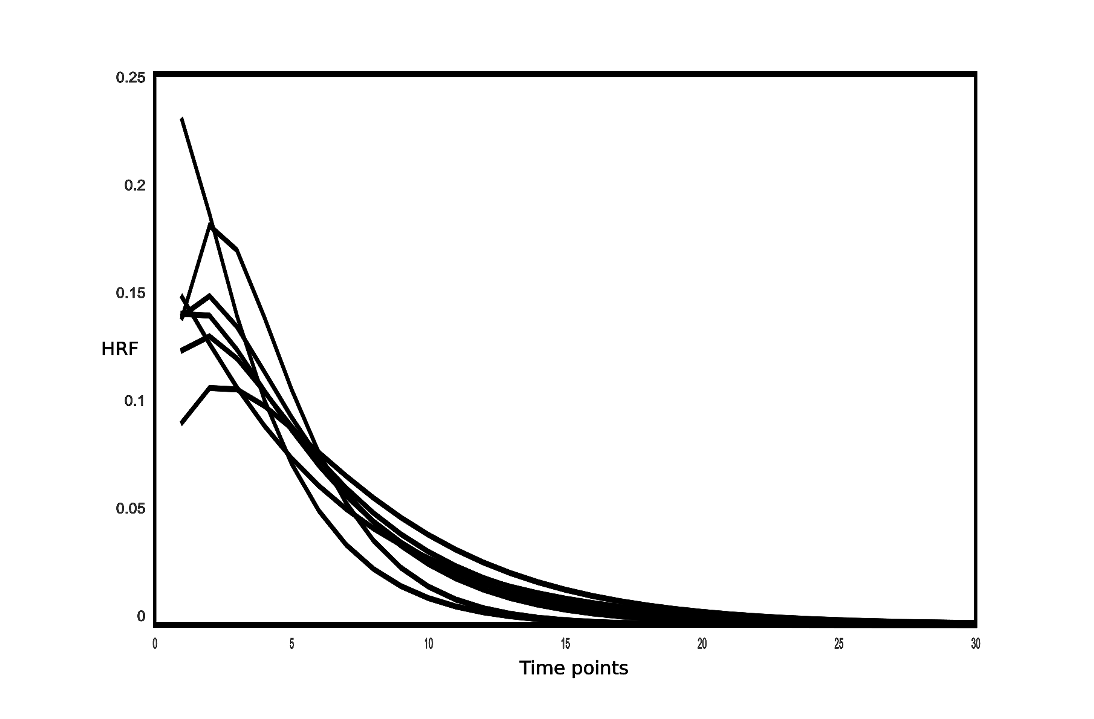
\includegraphics[width=\linewidth]{fig/encoding/gamma.eps}
	\caption{Comparison of haemodynamic response function learned by GAGamma encoding method for voxel 8 of subject 04847 across 7 different trials.}
	\label{fig:gamma}
\end{figure}


\subsubsection{Analysis of the Spike-train Encoded by GAGamma-16 Method}
Additionally, GAGamma-16 encoded spikes for the `seeing a picture', and the `reading a sentence' stimuli were independently analysed for interpreting the discriminating spatio-temporal influence of the spikes. As described earlier in the experimental protocol, the presentation of a certain stimulus within a trial follows an order, \emph{i.e.} for each stimuli class there exists subclasses of `presented first' or `presented second'. To analyse the effect of the first or second presentation of stimuli, the encoded dataset was separated into four classes, `picture presented first', `picture presented second', `sentence presented first' and `sentence presented second'. \figurenames \ref{fig:sub_04847} and \ref{fig:sub_07510} shows the comparison of the mean spike percentage across the trials for the four subclasses in subject 04847 and subject 07510. The points in the 3D plot correspond to the spatial location of the voxels. Each voxel belongs to two physiologically defined clusters or regions of interest, namely `CALC' and `LIPL.' The top row plots are the `picture' trials, and the bottom row trials are the `sentence' plots. The columns correspond to the stimulus (`picture' or `sentence') being presented first or second. The two clusters in each of the 3D plots relate to the two ROI's (top left is `LIPL' and bottom right is `CALC') of the brain structure. Functionally, the `CALC' region is responsible for central and peripheral vision whereas the `LIPL' region is related to visual attention. In both the subjects, `reading a sentence second' after `seeing a picture first' has more spike activity on average across the trials than the other way around, especially in the `LIPL' region. The mean spike activity in the `LIPL' is observed to be relatively higher ($0.59$ and $0.57$) when the subjects were `reading a sentence' than when the subjects were `seeing a picture' ($0.54$ and $0.55$). A two-sample T-test was conducted between the `seeing a picture' and the `reading a sentence' class in the `LIPL' region for the subjects to validate the previous result. The null hypothesis for the test conducted was the following, $H_0$: `there is no difference between the picture spike activity and sentence spike activity'. The null hypothesis was rejected at 5\% significance level with $p=5.27\times 10^{-18}$ for subject 04847 and with $p=7.05\times 10^{-12}$ for subject 07510. Hence, as per the T-test, the average spike activity across the trials over time for `seeing a picture' is significantly different from the average spike activity across trials over time for `reading a sentence'. Further, it must also be noted the sentences shown as part of the experiment are highly visual in nature (\emph{e.g.} `It is not true that the dollar is below the plus.') and requires a high image comprehension ability. This result is, therefore, consistent with the experimental results \citep{just2004imagery} obtained earlier which shows a greater degree of activation and functional connectivity in the `LIPL' region during cognitive tasks associated with high imagery sentence comprehension. This, in fact, also validates the ability of the proposed encoding algorithm to preserve the useful discriminatory information in the compressed encoded space of data.

\begin{sidewaysfigure}
	\subfloat[`seeing a picture' first during trial]{\label{fig:p11}
		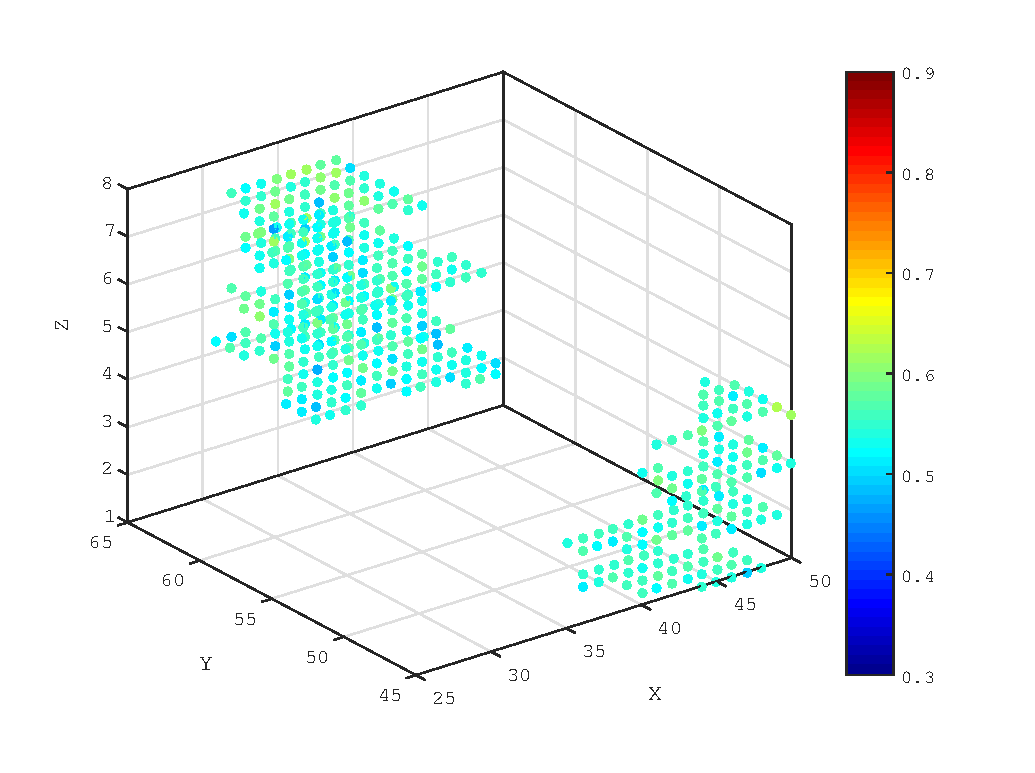
\includegraphics[width=0.42\textwidth]{fig/encoding/PICTURE_FIRST_04847.eps}}
	\subfloat[`seeing a picture' second during trial]{\label{fig:p12}
		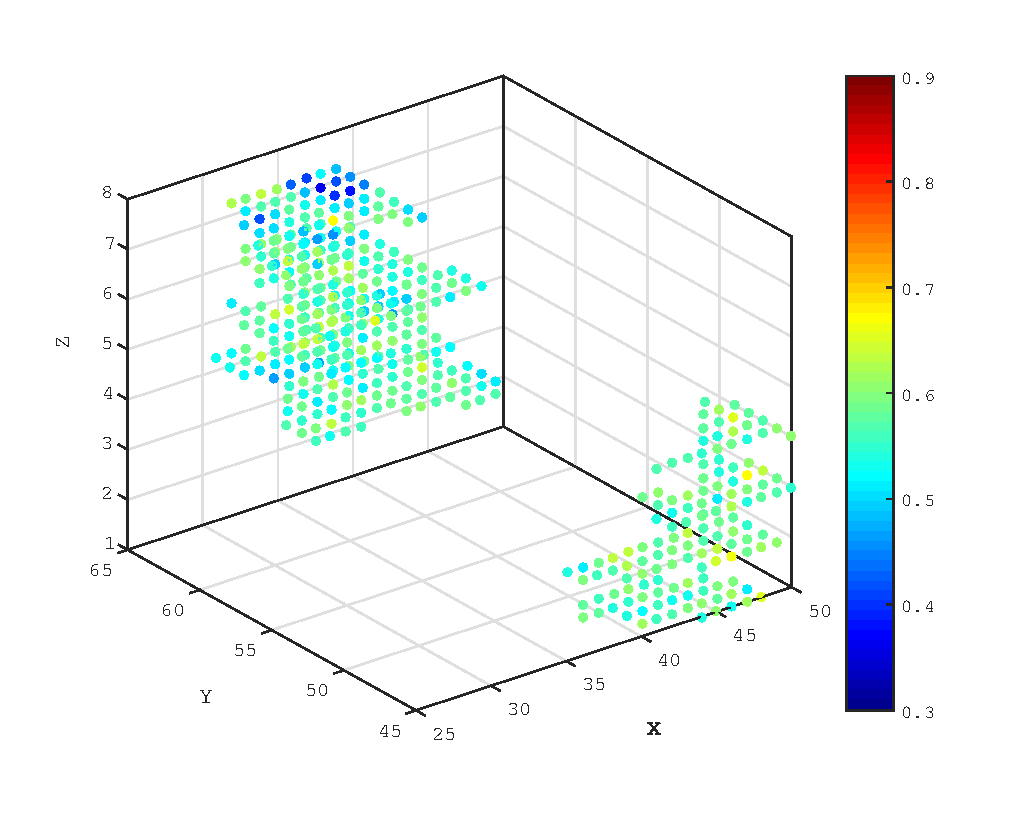
\includegraphics[width=0.42\textwidth]{fig/encoding/PICTURE_SECOND_04847.eps}}\\
	
	\subfloat[`reading a sentence' first during trial]{\label{fig:p13}
		\includegraphics[width=0.42\textwidth]{fig/encoding/SENTENCE_FIRST_04847.eps}}
	\subfloat[`reading a sentence' second during trial]{\label{fig:p14}
		\includegraphics[width=0.42\textwidth]{fig/encoding/SENTENCE_SECOND_04847.eps}}\\
	
	\caption{Comparative analysis of spike frequencies of the subject 04847 seeing picture vs. reading a sentence.}
	\label{fig:sub_04847}
\end{sidewaysfigure}

\begin{sidewaysfigure}
	\subfloat[`seeing a picture' first during trial]{\label{fig:p21}
		\includegraphics[width=0.42\textwidth]{fig/encoding/PICTURE_FIRST_07510.eps}}
	\subfloat[`seeing a picture' second during trial]{\label{fig:p22}
		\includegraphics[width=0.42\textwidth]{fig/encoding/PICTURE_SECOND_07510.eps}}\\
	
	\subfloat[`reading a sentence' first during trial]{\label{fig:p23}
		\includegraphics[width=0.42\textwidth]{fig/encoding/SENTENCE_FIRST_07510.eps}}
	\subfloat[`reading a sentence' second during trial]{\label{fig:p24}
		\includegraphics[width=0.42\textwidth]{fig/encoding/SENTENCE_SECOND_07510.eps}}\\
	
	\caption{Comparative analysis of spike frequencies of the subject 07510 seeing picture vs. reading a sentence.}
	\label{fig:sub_07510}
\end{sidewaysfigure}

% Please add the following required packages to your document preamble:
% \usepackage{booktabs}
\begin{table}
\centering
\caption{Average pairwise asynchronicity of three different voxels at the end of ten independent runs of GAGamma encoding.}
\label{tab:dist}
\begin{tabular}{@{}ccc@{}}
\toprule
\textbf{voxel ID} & $\mathbf{d_p}$ & $\mathbf{d_{vp}}$ \\ \midrule
$30$ & $24.18\pm 10.15$ & $0.23\pm 0.09$ \\
$468$ & $27.78\pm 11.96$ & $0.26\pm 0.10$ \\
$3429$ & $28.03\pm 11.31$ & $0.28\pm 0.11$ \\ \bottomrule
\end{tabular}
\end{table}

\tablename \ref{tab:dist} relates to the reproducibility of the spike-timings produced by the mixed integer genetic algorithm solver for the GAGamma encoding. The genetic algorithm being an evolutionary optimisation solver produces a non-reproducible result when on multiple iterations. Nevertheless, a pareto-optimal fitness value is guaranteed on each iteration. To validate the reliability of the GAGamma optimisation, in this instance, ten independent runs of GAGamma encoding was applied on three random voxels (30468 and 3429) from trial 12 of subject 04847. \tablename \ref{tab:dist} compares the similarity of the spike-trains produced by the GAGamma encoding using two spike-asynchronicity measures. They are the percentage asynchronicity $d_p$ and Victor Purpura distance $d_{vp}$ respectively. The Victor Purpura distance ($d_{vp}$) \citep{victor1997metric} metric is a cost based distance metric. The distance is defined by the minimum cost of converting one spike-train into the other using three operations: insertion (cost $1$); deletion (cost $1$); and shifting a spike by an interval $\delta t$ (cost $q|\delta t|$). For the smaller value of $q$ the distance metric approximates the spike count difference and hence supports rate coding. A higher penalty value of $q$, on the contrary, supports the number of non-coincidental spikes and hence temporal encoding. The comparison of the spike synchronicity using $d_p$ and $d_{vp}$ in \tablename \ref{tab:dist} shows that the spike-timings are correctly reproduced approximately $75\%$ of times.

\section{Summary and Conclusion}
In this Chapter, the focus was on using temporal encoding as a framework to concisely represent large volumes of data by spike-timings. By doing so, the existing discriminatory spatio-temporal information was preserved. In this regard, apart from using the existing temporal encoding techniques, a novel temporal encoding framework was formalised and a specific encoding algorithm for fMRI data, called GAGamma, was proposed. The experimental result on benchmark fMRI dataset shows the superiority of the temporal encoding algorithms, such as GAGamma and BSA, to succinctly represent the discriminatory information in the compressed encoded spike space without losing any appreciable amount of information. Thus, it achieves comparable or superior pattern recognition performance. It can be argued that the flexibility of the proposed encoding framework lies in its ability to inject known structure information about the data source and thus, provide the compression/encoding algorithms sufficient redundancy to represent the large dataset in an optimally concise manner. 

\pagebreak
\section{Contributions and Publications}
\begin{tcolorbox}[colback=black!5,colframe=black!40!black,title=Contributions]
	\begin{enumerate}
		\item A generalised \emph{a priori} knowledge driven optimisation framework for spike-time encoding of continuous data was formalised.  
		\item To elaborate the characteristics of this framework, a realisation of the proposed framework, namely GAGamma, was proposed for the purpose of encoding fMRI data using \emph{a priori} knowledge of the data source.
		\item The proposed encoding algorithm was applied and compared with state of the art encoding algorithms on a benchmark pattern recognition problem involving fMRI data. The results showed, in general, the uniqueness of the proposed temporal encoding framework not only lies in its ability to significantly compress the data, but also in keeping the discriminatory information intact, which is extremely useful for pattern recognition tasks. 
	\end{enumerate}
	
\end{tcolorbox}

\begin{tcolorbox}[colback=black!5,colframe=black!40!black,title=Publications]
	\begin{enumerate}
		\item \textbf{Sengupta, N.}, \& Kasabov, N. (2017). Spike-time encoding as a data compression technique for pattern recognition of temporal data. Information Sciences,  406, 133-145.	
		
		\item \textbf{Sengupta, N.}, Scott, N., \& Kasabov, N. (2015). Framework for knowledge driven optimisation based data encoding for brain data modelling using spiking neural network architecture. In Proceedings of the Fifth International Conference on Fuzzy and Neuro Computing (FANCCO-2015) (pp. 109-118). Springer, Cham.
	\end{enumerate}
\end{tcolorbox}
\chapter{Orientation Influence Driven Spike-Time Dependent Plasticity Learning: A Novel Unsupervised Learning Algorithm for Integrating Spatial, Temporal and Orientation Information}
\label{chap:multimodal}
\section{Introduction}
\label{sec:introduction}
In the recent past, non-invasive brain data collection techniques such as functional magnetic resonance imaging (fMRI), electroencephalography (EEG), diffusion tensor imaging (DTI) and others have made significant contributions to understanding various structural and functional properties of the human brain. There has been consistent development in data sampling technology over the past few years which has enabled simultaneous sampling of multiple modalities of brain data while a subject performs or does not perform a task. This provided an opportunity to perform pattern recognition using large quantities of such data. It is evident that each data modality provides a unique but limited perspective of the brain. In the past, these data modalities were used independently for pattern recognition and overlooked the joint information present in the data \citep{sui2012review}. Algorithms with the ability to extract and integrate relevant information from various data sources into a single model are crucial not only for predictive modelling but also in terms of understanding the spatio-temporal relationships within the data.

Structural dysconnectivity, as measured by DTI, has been demonstrated in several psychiatric disorders and has been shown to reflect functional dysconnectivity in some cases \citep{greicius2009resting, stephan2009dysconnection}. In accordance with these theories, it would be appealing to incorporate dysconnectivity information into any algorithm that is designed to classify or predict outcomes in people with psychiatric disorders. This Chapter discusses the steps that have been undertaken to develop a new algorithm that can incorporate orientation information from DTI along with the EEG/fMRI activity data as a data fusion approach. The most commonly used method of integrated data analysis for this kind of problem is by “converging evidence” \citep{horwitz2002can}. Typically, each data type is analysed separately, and the results from other analysis that support one's findings are discussed. \citet{horwitz2002can} also put forth discussions about an alternative data fusion analysis called “computation neural modelling”. This is done by creating biologically realistic neural network models, where each network simulates data of a certain type and is compared with observed data. One major setback of this paradigm of data analysis is that the hypothesis driven neural network model is built under several assumptions for simulated data generation. Hence, it would be difficult to know whether a disagreement between observed and simulated data is due to the assumptions in the model, or simply wrong. A comprehensive review of the research in the direction of multi-modal brain data analysis is summarised by \citet{sui2012review}. Some prominent work includes integration of fMRI/EEG \citep{valdes2009model}, fMRI/MEG \citep{plis2011effective}, fMRI/DTI \citep{stampfli2008combining, kleiser2010impact} and fMRI/gene expression \citep{yang2010hybrid}. There is a third alternative for multi-modal data integration known as data fusion, which is a more data driven approach. Direct data fusion encompasses the technique of directly fusing multiple datasets using statistical and machine learning algorithms. The data-driven methods span across the domain of the combined blind source separation techniques such as Independent Component Analysis \citep{calhoun2009review, teipel2010white} and its variants, multi-modal Cross-Correlation Analysis \citep{correa2008canonical,correa2010multi,correa2008examining}, Partial Least Squares \citep{chen2009linking}, and others. 

\section{fMRI}

\begin{figure}
	\centering
	\includegraphics[width=0.7\linewidth]{fig/fmridti/fMRI_scanner.jpg}
	\caption{fMRI scanning device (source \citet{fmriscanner}).}
	\label{fig:fmri_scanner}
\end{figure}

Functional magnetic resonance imaging (fMRI) is a form of magnetic resonance imaging that takes advantage of magnetic susceptibility artefacts caused by the deoxygenated haemoglobin in the brain. Magnetic susceptibility measures the magnetic properties of the interaction between a tissue or other substance and the in-scanner magnetic field strength. Magnetically susceptible materials distort the homogeneity of a magnetic field: materials with negative magnetic susceptibility are known as diamagnetic, and those with positive magnetic susceptibility are referred to as paramagnetic. Introduction of a paramagnetic substance, such as deoxyhaemoglobin, into the scanner magnetic field causes variability in field strength, spin dephasing, geometric distortion and loss of signal; fMRI exploits this property by measuring changes in the relative ratio of oxygenated (diamagnetic) to deoxygenated (paramagnetic) haemoglobin in the blood. 

fMRI measures the haemodynamic response to neuronal excitation and is therefore a secondary measure of neuronal activity. As the metabolic demands of neurons increase (as observed during task performance), astrocytes are signalled to produce prostaglandin E2 and epoxyeicosotrienoic acids, which diffuse to arteriolar smooth muscle and cause vasodilation \citep{hamilton2010pericyte}. Independently, adenosine, a breakdown product of adenosine triphosphate (ATP) produced during periods of high metabolic demand signals pericytes (contractile cells surrounding capillaries) to relax, permitting increased blood flow through capillaries \citep{hamilton2010pericyte}. This increased blood flow delivers high concentrations of oxygenated haemoglobin and glucose to the activated region, increasing the ratio of oxygenated to deoxygenated haemoglobin. As discussed above, deoxyhaemoglobin is paramagnetic and causes dephasing and signal loss in the MR image. Increasing the ratio of oxyhaemoglobin to deoxyhaemoglobin reduces signal loss, because oxyhaemoglobin is diamagnetic. It is this decreased signal loss, corresponding to the peak of the haemodynamic response function (HRF), that is measured during fMRI experiments. This is referred to as the blood oxygen-level dependent (BOLD) signal. Importantly, the HRF produces
only a $1-2\%$ change in signal following a single stimulus. For this reason, it is required that data be collected over a long period of time so that the signal to noise ratio can be improved.
fMRI may be acquired during performance of a cognitive task or during rest. During rest, the brain exhibits patterns of spontaneous activity that coincide with those present during task performance \citep{smith2009correspondence}, making resting-state fMRI (rs-fMRI) an excellent tool for investigating functional brain connectivity. In a standard setup, fMRI data is collected using an MRI device such as the one shown in \figurename \ref{fig:fmri_scanner}. Each fMRI scan is visualised as sequence of 2D slices of a 3D image. The pixel colours represents the indirect measure of neural activity. An example of fMRI data visualisation is shown in \figurename \ref{fig:fmri_images}. Each image in \figurename \ref{fig:fmri_images} is showing a single slice horizontal view of the 3D image.

\begin{figure}
	\centering
	\includegraphics[width=0.7\linewidth]{fig/fmridti/fmri.png}
	\caption{Example of fMRI data represented as a sequence of images (source \citet{quarantelli2013default}).}
	\label{fig:fmri_images}
\end{figure}

\section{DTI and Tractography}
DTI is a magnetic resonance imaging technique that uses immense gradient amplitudes together with spin-echo or gradient-echo EPI sequences to provide a measure of the relative diffusion of molecules in tissues. In DTI, each voxel of the MR image has one or more pairs of parameters: a rate of diffusion and a preferred direction of diffusion described in terms of three-dimensional space for which that parameter is valid. 

The diffusion of hydrogen within a voxel is described by the diffusion tensor $D$ as represented by \equationname \ref{eq:dti_ellipsoid}. $D$ is a reciprocal matrix, with six independent scalar elements ($D_{xx}$, $D_{yy}$, $D_{zz}$, $D_{xz}$, $D_{xy}$, $D_{yz}$). The six unique elements of the tensor are the coefficients of the ellipsoid equation given by $D_{xx}x^2 + D_{yy}y^2 + D_{zz}z^2 + D_{yx}yx + D_{zx}zx + D_{xy}xy = 1$. This equation can also be expressed in terms of orthogonal Eigenvectors $\sigma$ and their respective eigenvalues $\lambda$. These variables describe the elements of the diffusion ellipsoid as shown in \figurename \ref{fig:dti_ellipsoid}.
\begin{equation}
D=\begin{pmatrix}
	D_{xx}       & D_{xy} & D_{xz} \\
	D_{xy}       & D_{yy} & D_{yz}  \\
	D_{xz}       & D_{yz} & D_{zz} 
\end{pmatrix}=
\begin{pmatrix}
\sigma_1\\
\sigma_2\\
\sigma_3
\end{pmatrix}
\begin{pmatrix}
\lambda_1 & 0 & 0 \\
0 & \lambda_2 & 0  \\
0 & 0 & \lambda_3 
\end{pmatrix}
\begin{pmatrix}
\sigma_1 & \sigma_2 & \sigma_3
\end{pmatrix}
\label{eq:dti_ellipsoid}
\end{equation}

Isotropic diffusion within a voxel causes the diffusion ellipsoid to take a spherical shape with $\lambda_1=\lambda_2=\lambda_3$. In contrast, restriction of diffusion in certain directions leads to an elevated eigenvalue coupled with the principal diffusion direction as opposed to those corresponding to the secondary and tertiary diffusion direction. From the tensor equation depicted in \equationname \ref{eq:dti_ellipsoid}, a number of metrics corresponding to the properties of diffusion in the voxel can be derived. $\lambda_1$ corresponds to the primary direction of diffusion (principle eigenvector; $\sigma_1$) is referred to as the axial diffusivity (AD). Radial diffusivity (RD) is the mean of $\lambda_2$ and $\lambda_3$ and reflects the diffusion behaviour transverse to the axonal path. 
\begin{figure}
	\centering
	\subfloat[The primary, secondary and tertiary diffusion directions described by the Eigenvectors of \equationname \ref{eq:dti_ellipsoid}.]{\includegraphics[width=0.7\textwidth]{fig/fmridti/ellipsoid_1.eps}}\\
	\subfloat[The primary, secondary and tertiary Eigen values described in \equationname \ref{eq:dti_ellipsoid}.]{\includegraphics[width=0.7\textwidth]{fig/fmridti/ellipsoid_2.eps}}
	\caption{Visual intuition of the ellipsoid representation of a diffusion tensor voxel.}
	\label{fig:dti_ellipsoid}
\end{figure}

From the raw data, it is possible to determine fractional anisotropy but not the fibre orientation. Diffusion tensor information can also be used to reconstruct white matter bundles in the brain. This technique is termed tractography. Fibre tractography is a very elegant method for delineating individual fibre tracts from diffusion images. Tractography uses diffusion orientation information from tensor imaging to calculate the direction of fibre bundles in-vivo. In deterministic, or streamline tractography, the local tract direction is defined by the major eigenvector of the diffusion tensor \citep{alexander2010deterministic}. This causes issues in voxels with crossing, kissing or splitting fibres. However, as the algorithm is only capable of estimating one fibre orientation \citep{alexander2010deterministic}, probabilistic tractography addresses these issues by estimating the orientations of two or three different fibre populations within a single voxel \citep{behrens2007probabilistic}. Thereafter, at every voxel, the algorithm estimates the most probable fibre orientation and also provides a distribution representing the probability that every other orientation lies along that fibre. This process is repeated many times, each time using a slightly different orientation (according to its likelihood). The integration of all estimates provides a collective measure of connection probability along each tract \citep{behrens2007probabilistic, behrens2003characterization}. \figurename \ref{fig:diff_mri} shows an example of a diffusion MRI image of the human brain.

\begin{figure}
	\centering
	\includegraphics[width=\textwidth]{fig/fmridti/dmri.png}
	\caption{Orientation information from DTI image. Left image shows an axial slice of a single subject's DTI data, registered to structural and MNI standard space. The Right image shows a close-up of the right posterior corpus callosum. Directions corresponding to each colour are as follows: Red - left to right/right to left, green - anterior to posterior/posterior to anterior and blue - superior to inferior/inferior to superior (source \citet{dtiwiki}).}
	\label{fig:diff_mri}
\end{figure}

\section{NeuCube Architecture for Integrating Spatial, Temporal and Orientation Information}

\subsection{Formalisation of the Machine Learning Problem}
The machine learning problem here is to learn a functional mapping of $f(D_{seq}, D_{stat})\rightarrow C$, given a set of training samples  $<D_{seq},D_{stat}, C>$, so that the spatial temporal and orientation information present in $D_{seq}$ and $D_{stat}$ are used to not only increase prediction performance, but also impart robustness to the model. Here $D_{seq}$ and $D_{stat}$ represents the fMRI/EEG and DTI data respectively.

\subsection{NeuCube Personalised SNNc Architecture}
\label{sec:neucube_person}
Here, a personalised SNNc based NeuCube architecture is proposed for the purpose of learning from multi-modal information. The personalised SNNc based NeuCube architecture is a modification of the NeuCube architecture described in Section \ref{sec:neucube_estdm} and depicted in \figurename \ref{fig:neucube_archit}. Before proposing the modified architecture, it is necessary to elaborate certain characteristics of the SNNc in a canonical setting.

\paragraph{Saturation behaviour of canonical NeuCube SNNc:} The classical NeuCube architecture shown in \figurename \ref{fig:neucube_archit} is made up of a single instance of encoder layer, SNNc layer and supervised readout layer. The instances of these layers are initialised before the training process and data is passed through sequentially over time for: (1) Encoding layer to continuously encode the data into spike-timings; (2) SNNc layer to digest the data and update its state; and (3) supervised readout layer to digest the transformed spike-train and create instances in the data space for the K-NN algorithm to act on. NeuCube is a pattern recognition system that learns continuously from data. During the course of development of NeuCube, it is observed that in a vanilla setting, learning continuously from streaming input data has some undesirable effects on the run-time efficiency and performance over time. Upon analysis, it was found this behaviour relates to the single instantiation of the NeuCube SNNc layer. 

To further describe this behaviour, the spike density of SNNc can be defined as the number of neurons that fire at a certain time instance. It is observed that as input data is fed into the SNNc over time, the probability of the neurons in the SNNc firing increases. The spiking neuron of course has a mechanism, such as refractoriness, to avoid continuous spiking; however, over time, periodicity in spike density cannot be avoided. To demonstrate this statement, a set of experiments were conducted using synthetically generated spike data. 

In the experimental setup, a small SNNc was initialised having $27$ neurons. The neurons were spatially distributed in a $3\times 3\time 3$ grid. The network of neurons were connected following the SWC algorithm ($r_{thr}=0.3$). For input data, random input spikes (with spiking probability $0.3$) data $D_{seq}=\{0, 1\}^{200\times 4}$ were synthetically generated for each sample. \tablename \ref{tab:saturation} enlists three instances of the experiment wherein the canonical SNNc unsupervised learning algorithm was run using varying sample sizes and hyperparameter values. At the end of the SNNc simulation, the spike-rate over time (or samples as samples are presented over time) was plotted. It can be observed that irrespective of the hyperparameter settings, a periodicity/total saturation in spike-rate is seen in the SNNc. As a consequence, the spiking patterns after a certain number of sample presentations becomes predictable and does not relate to the variabilities in the sample any more. This fact can be verified from the `sample distance matrix' column where the pairwise hamming distance matrix was plotted across the sample output of the SNNc. The colours (red is high and blue is low) in the plot represents the hamming distance between two samples. It must be noted that the hamming distance between samples not only considers how many times SNNc has spiked for a sample, but also considers when the neurons have spiked. It can be observed there is a lot of variability in the similarity values initially, but as more samples are presented, the spike patterns become more and more similar leading to very small values of dissimilarity. 

The point of including the SNNc layer is to improve pattern formation by expanding it into higher dimensional space. However, the behaviour described above does have a significant impact on pattern generation capabilities of the canonical NeuCube SNNc beyond a certain time. This can be defined as saturation threshold time. There are two directions where research can traipse in order to resolve or further analyse this issue:

\begin{itemize}
	\item Improve the SNNc mechanisms and principles to keep it within sub-threshold limit. In this setting, a single instance of the SNNc can be simulated lifelong without reduction in pattern generation abilities.
	\item Minimise the impact of saturation by using multiple instances of the SNNc and control the sub-threshold state using the hyperparameter values. This approach was used in this work.
\end{itemize}          

\begin{sidewaystable}
	\centering
	\caption{Experimental results showing saturation characteristics of canonical NeuCube SNNc.}
	\label{tab:saturation}
		\begin{tabular}{@{}|l|l|l|l|l|l|l|@{}}
			\toprule \toprule
			\# samples & $v_{thr}$ & $\eta_{thr}$ & $\kappa$ & sample vs spike rate & Hamming distance matrix & saturation type \\ \midrule
			50 & 0.5 & 0 & 0.1 & \includegraphics[scale=0.4]{fig/fmridti/sat1.eps}  & \includegraphics[scale=0.6]{fig/fmridti/sat1d.eps} & total \\ \midrule
			500 & 10 & 0 & 0.1 & \includegraphics[scale=0.4]{fig/fmridti/sat2.eps} & \includegraphics[scale=0.6]{fig/fmridti/sat2d.eps}  & periodic \\ \midrule
			200 & 1 & 15 & 0.1 & \includegraphics[scale=0.4]{fig/fmridti/sat3.eps} & \includegraphics[scale=0.6]{fig/fmridti/sat3d.eps} & periodic \\ \bottomrule \bottomrule
		\end{tabular}%	
\end{sidewaystable}

The personalised SNNc based NeuCube architecture is depicted in \figurename \ref{fig:personaliosed_arch}. In the personalised SNNc approach, usage of multiple instances of SNNc was proposed. In this approach one instance of SNNc is simulated per sample along with a single instance of the encoding layer and supervised readout layer. In this setup, each sample of input data is fed into a unique pre-initialised personal SNNc. The personal SNNc acts as a filter which evolves over time to capture the spatio-temporal relationships within a sample in the synaptic strengths. The knowledge of finite time horizon means the SNNc instance can be kept in a sub-saturation state by controlling the hyperparameter ranges. The other advantage of the personalised SNNc architecture is the ability to avoid the sequential sample presentation bias that may exist if all the samples are fed into a single instance of the SNNc. This means the sequence of the sample presentation does not have any impact on spike patterns generated by the SNNc. The other important aspect of the proposed personalised SNNc architecture is the ability to incorporate multi-modal nature of the input data which will be discussed further.   

\begin{sidewaysfigure}
	\includegraphics[width=0.8\linewidth]{fig/fmridti/neucube_personalised_arch.pdf}
	\caption{Proposed NeuCube personalised SNNc architecture.}
	\label{fig:personaliosed_arch}
\end{sidewaysfigure}


\subsection{Multi-modal Information Integration in SNNc Using Orientation and Spike-time Data}
\label{sec: SNNc}
In this Section, the proposed adaptations of the canonical SNNc unsupervised learning algorithm mentioned earlier in Section \ref{sec:neucube_snnc_learning}, for the purpose of fusing dynamic spatio-temporal and static orientation information from brain data, will be discussed. 

\subsubsection{SNNc Architecture, Mapping and Initialisation}
The SNNc architecture, as described elaborately in Section \ref{subsec:SNNc_init}, are spatially arranged (in three dimensions) set of neurons, partially connected by recurrent synapses forming a directed incomplete and acyclic graph $G=\{M, C, W\}$. The symbols and formalisations are consistent with Chapter \ref{chap:large_snn} unless otherwise stated. The neurons within the network are input or spiking types. The spatial arrangement of the neurons follow a natural ordering and in the case of brain data, integration takes a brain-like shape. The connections of the network are established following the standard SWC \citep{kasabov2014evolving} algorithm.  

\subsubsection{Neuron Dynamics}
The SRM model has been used for implementing the leaky integrate and fire like behaviour of a neuron. The SRM neuron model is used to adapt the membrane potential $v(t)$ of a neuron over time. This neuron model specifies the membrane potential as the sum of: (1) temporal integration of the PSPs and (2) the refractoriness. The PSP kernel $\epsilon_0$ is a function of $t-t^f$, representing the PSP trace over time generated by the firing of neuron $j$ over time. $\tau_m$  is known as the membrane constant which controls the decay rate of the PSP. In the present experiments, a constant $\tau_m = 0.5$ has been used. This means the influence of a pre-synaptic spike diminishes from maximum to minimum within approximately five discrete time intervals. For a more detailed explanation and behaviour of the neuron dynamics, see Section \ref{subsec:SNNc_neuron_model}.

\begin{equation}
\begin{matrix}
\displaystyle v_i(t)=v_{rest}+\sum_{j\in \Tau_i }w_{ji}\sum_{t_j^f\in F_j}\epsilon_0(t-t_j^f)+\eta(t-t_i^f) \\ \\

\epsilon_0(t-t_j^f)=\exp(-\frac{t-t_j^f}{\tau_m})\mathcal{H}(t-t_j^f)\\ \\

\mathcal{H}(t-t_j^f)=\left\{
\begin{array}{@{}cc@{}}
1, & \text{if}\ t-t_j^f\geq 0 \\
0, & \text{otherwise}
\end{array}\right.  \\ \\

\eta(t-t_i)=\left\{
\begin{array}{@{}cc@{}}
-\infty, & \text{if}\ t-t_i^f<\eta_{thr}\\
0, & \text{otherwise}
\end{array}\right.

\end{matrix}
\label{eq:SRM_multimodal_neucube}
\end{equation} 

\paragraph{Python implementation:} The neuron model dynamics has been implemented in python $v3.5$. The neuron model dynamics were implemented as part of the $LeakyIntegrateAndFire$ class shown below. The $simulate()$ method is implemented to simulate the neuron dynamics using the input $spike\_train$ and pre-synaptic connection weights $weight$ and hyperparameter $tau$.
\begin{lstlisting}[language=Python, caption={Python code for NeuCube modified SRM neuron model}]
class LeakyIntegrateAndFireNeuron:
	def __init__(self, predecessor_count, potential_threshold, refractory_threshold, potential_resting, spike_history_length):
		self.predecessor_count = predecessor_count
		self.refractory_threshold = refractory_threshold
		self.potential_threshold = potential_threshold
		self.potential_resting = potential_resting
		self.spike_history_length = spike_history_length
		self.time = 0
		# initialise neuron state
		self.potential = self.potential_resting
		self.refractory_state = 0
		self.potential_state_history = [self.potential]
		self.spike_history = np.zeros((self.spike_history_length, self.predecessor_count), dtype=int)

	@staticmethod
	def spike_response_kernel(current_time, spike_time, tau):
		time_diff = current_time - spike_time
		potential = np.exp(-time_diff / tau)
		return potential

	def simulate(self, spike_train, weight, tau):
		self.time += 1
		self.spike_history = np.delete(self.spike_history, 0, axis=0)
		self.spike_history = np.append(self.spike_history, [spike_train], axis=0)
		current_time = self.spike_history_length
		potential = self.potential
		spike = 0
		if self.refractory_state == 0:
			for k in np.arange(current_time):
				count = np.count_nonzero(self.spike_history[k, :])
				indices = np.nonzero(self.spike_history[k, :])
				for i in range(count):
					w = weight[indices[0][i]]
					potential += w * self.spike_response_kernel(current_time=current_time - 1, spike_time=k, tau=tau)
			self.potential = potential
			self.potential_state_history.append(self.potential)
			if self.potential > self.potential_threshold:
				self.refractory_state = self.refractory_threshold
				self.potential = self.potential_resting
				spike = 1
		else:
			self.refractory_state = max(0, self.refractory_state - 1)
			self.potential = max(self.potential_resting, self.potential)
			self.potential_state_history.append(self.potential)
	return spike
	
\end{lstlisting}

\subsubsection{Adaptation of Synaptic Strengths of the SNNc}
\label{subsec:SNNc_learning}
The unsupervised learning algorithm in the SNNc is the most important aspect of the proposed architecture for integrating multi-modal information. In a neural network paradigm, learning is achieved through the synaptic strength updates of the network. The learning behaviour of the SNNc can be explained using the learning model of a single spiking neuron. Considering the single neuron architecture, as shown in \figurename \ref{fig:neuron_architecture}, the unsupervised learning problem is the a scheme of updating the $w_{ji}$'s by $\Delta w_{ji}(t)$ over the simulation time $T$. In a recurrent SNNc layer, the aim is to learn dynamic influence from dynamic data (fMRI) and static orientation influence from static data (DTI).  


\subsubsection{Dynamic Influence from fMRI/EEG}
\label{subsec:phi}

In the majority of the machine learning applications, models are trained on static data, where a sample is represented by a vector of numbers $\mathbf{d}=\{d_1,d_2,\cdots\}$, where each of the elements within the tuple $d$ represents the scalar value of a particular feature. However, in this case with fMRI or EEG data, a sample is represented by a matrix $\mathbf{D_{seq}=\{d_1, d_2,\cdots, d_n\}}$, where $\mathbf{d_i}=\{d_i(1), d_i(2),\cdots d_i(t)\}$. The sample representation is not only multidimensional but also is ordered in time (sequence). Learning from these types of data in machine learning is known as sequence learning and techniques, like the hidden Markov model and flavours of recurrent neural network have shown promise in learning from such sequences. In this instance, an unsupervised sequence learning algorithm will be described that is within the NeuCube SNNc layer and utilises the sequential information as part of its learning mechanism. The sequential information within the SNNc architecture is named as the dynamic influence and is denoted by $\phi$.        

The dynamic influence from the spike-time data using the STDP learning algorithm was modelled. As discussed elaborately in Section \ref{subsec:STDP}, STDP is a temporally asynchronous form of Hebbian learning ("neurons wire together, if they fire together") \citep{hebb1949organization} induced by the temporal correlation of the spikes. Due to the online nature of the learning within the SNNc layer, the canonical online formulation of the STDP learning rule have been used. \citet{sjostrom2010spike} proposed the on-line STDP update rule by modifying the canonical STDP rule. In the on-line setting, the $\phi_{ji}$ is calculated every time a neuron $i$ fires a spike or receives a spike from neuron $j$. \equationname \ref{eq:multimodal_stdp_online} formalises the weight update rule that was used to calculate the dynamic influence. The first term in the right hand side of \equationname \ref{eq:stdp_online} corresponds to the LTP update and is calculated when neuron $i$ fires a spike at time $t$. The second term is the LTD update and is calculated when neuron $i$ receives a spike from neuron $j$ at time $t$. 


\begin{equation}
\phi_{ji}(t) = \sum_f \kappa_+\exp(-(t-t_j^f))-\sum_g \kappa_- \exp(-(t-t_i^g))
\label{eq:multimodal_stdp_online}
\end{equation}

\paragraph{Python implementation:} The python implementation of \equationname \ref{eq:multimodal_stdp_online} is given below. The $STDP()$ method takes the pre- and post-synaptic spike history $t_j^f$s and $t_i^g$s along with the learning rate hyperparameter $\kappa$ to generate the dynamic influence $phi$. 

\begin{lstlisting}[language=Python, caption={Python code for calculating dynamic influence}, label={list:stdp}]
def STDP(pre_synaptic_spike_history, post_synaptic_spike_history, kappa):	
	assert isinstance(pre_synaptic_spike_history, list)
	assert isinstance(post_synaptic_spike_history, list)
	if len(pre_synaptic_spike_history) != len(post_synaptic_spike_history):
	raise ValueError("Length mismatch of pre and post synaptic spike history!!")
	pre_synaptic_spike_energy = 0
	post_synaptic_spike_energy = 0
	importance_of_LTP = 0.3
	importance_of_LTD = 0.3
	time_history = len(pre_synaptic_spike_history)
	pre_synaptic_spike_history = np.asarray(pre_synaptic_spike_history)
	post_synaptic_spike_history = np.asarray(post_synaptic_spike_history)
	"""
	calculation of LTD
	"""
	if pre_synaptic_spike_history[time_history - 1] == 1:
		post_spike_indices = np.nonzero(post_synaptic_spike_history)[0]
		k = kappa * np.exp(-(1 - importance_of_LTD) * ((time_history - 1) - post_spike_indices))
		pre_synaptic_spike_energy = np.sum(k)
	
	"""
	calculation of LTP
	"""
	if post_synaptic_spike_history[time_history - 1] == 1:
		pre_spike_indices = np.nonzero(pre_synaptic_spike_history)[0]
		k = kappa * np.exp(-(1 - importance_of_LTP) * ((time_history - 1) - pre_spike_indices))
		post_synaptic_spike_energy = np.sum(k)
	phi = post_synaptic_spike_energy - pre_synaptic_spike_energy
	return phi
\end{lstlisting}


\begin{figure}
	\centering
	\includegraphics[width=\linewidth]{fig/fmridti/STDP.eps}
	\caption{Plot of the STDP weight update as a function of the relative time difference of the pre and post synaptic spikes. The data for this plot was generated using code snippet \ref{list:stdp} with hyperparameter $\kappa_+=\kappa_-=0.5$.}
	\label{fig:stdp}
\end{figure}



\subsubsection{Static Orientation Influence from DTI Tractography Data}

The present study has used the DTI data in the form of orientation vectors representing mean orientation of the fibre tract at different voxel locations. The process of generating the orientation data from a DTI image is described later in Section \ref{subsec:schizophrenia_method}. The orientation vector of a sample DTI image is represented by a matrix $\mathbf{D_{stat}} \in \mathbb{R}^{|N|\times 3}$, where each feature/voxel is made up of a 3D vector describing the primary orientation of the fibre in the Cartesian coordinate system.   
\begin{figure}
	\centering
	\includegraphics[width=\linewidth]{fig/fmridti/angular_influence.png}
	\caption{Example of a pre-synaptic neuron $j$ connected to two post synaptic neurons $i_1$ and $i_2$. Each neurons spatial location is defined by the polar coordinates $(r, \alpha$).}
	\label{fig:ang_inf}
\end{figure}

Here, the interest lies in establishing a learning rule that does not only utilises dynamic data influence as described in Section \ref{subsec:phi}, but can also make use of the static orientation influence from the DTI data. The intuition behind the orientation influence can be explained again by a small SNNc architecture consisting of three neurons as shown in \figurename \ref{fig:ang_inf}. The figure shows a single pre-synaptic neuron $j$ connected to two post synaptic neurons $i_1$ and $i_2$. The important aspect to note here is that the neurons in this diagram have spatial allocations contrary to the one in \figurename \ref{fig:neuron_architecture}. The location of the neurons are defined by the radial and the angular coordinates in the polar coordinate system. Now, the intent is to measure the orientation influence $\psi$ of neuron $j$ on neurons $\{i_1, i_2\}$. The neuron $j$ will be referred to as the pivot neuron. The orientation vector of the pivot neuron (from DTI data) is be represented by $(r_j, \alpha_j)$. The orientation influence of the pivot neuron on the post-synaptic neurons $\{i_1,i_2\}$ is defined by the angular proximity of the pivot neuron's DTI orientation vector to the synaptic orientations of the neuron pairs.  In that way, as per the hypothesis, the pivot neuron wields a stronger angular influence on the neurons that lie in closer angular proximity to the orientation vector of the pivot neuron. Therefore in \figurename \ref{fig:ang_inf}, the orientation influence of neuron $j$ can be arranged as $i_1>i_2$ due to the angular proximity of $i_1$ and $j$ being greater than $i_2$ and $j$. 

Even though a 2D vector space has been used for explaining the intuition of angular influence, the SNNc neurons reside in a 3D space. The intuition can be extended to the 3D vector space by adding another dimension in the coordinate system. In 3D, the spherical coordinates of a point are given by $(r,\alpha, \beta)$, where $r$ is the scalar distance of the point from the centre, $\alpha$ and $\beta$ are the elevation and azimuth angle from the centre. A Gaussian radial basis (GRB) kernel has been utilised to realise the elevation and azimuth orientation influences given the elevation and azimuth data of the neurons. $\psi$ is calculated as the mean of azimuth and elevation influences between pre- and post-synaptic neurons $j$ and $i$ according to \equationname \ref{eq:angular_influence}.

\begin{equation}
\begin{matrix}
\psi_{ji}=\frac{\psi_{ji}^\alpha+\psi_{ji}^\beta}{2} \\ \\

\psi_{ji}^\alpha=\exp(\frac{||\alpha_{ji}-\alpha_j^{dti}||^2}{2\gamma^2})\\ \\

\psi_{ji}^\beta=\exp(\frac{||\beta_{ji}-\beta_j^{dti}||^2}{2\gamma^2})

\end{matrix}
\label{eq:angular_influence}
\end{equation} 

\paragraph{Python implementation:} The python implementation of \equationname \ref{eq:angular_influence} is given below. The $angular\_influence()$ method takes the coordinates of two neurons and the orientation information, and outputs the orientation influence $psi$. 

\begin{lstlisting}[language=Python, caption={Python code for calculating static orientation influence}]
def angular_influence(pivot_coordinate, sphere_coordinate, elevation_angle, azimuth_angle):
	assert isinstance(pivot_coordinate, np.ndarray)
	assert isinstance(sphere_coordinate, np.ndarray)
	assert isinstance(elevation_angle, float)
	assert isinstance(azimuth_angle, float)
	
	standard_deviation = 8	
	relative_sphere_coordinate = np.subtract(sphere_coordinate, pivot_coordinate)
	radius, elevation, azimuth = cart2sph(relative_sphere_coordinate[0], relative_sphere_coordinate[1], relative_sphere_coordinate[2])	
	el_prob = radial_decay(elevation, elevation_angle, standard_deviation)
	az_prob = radial_decay(azimuth, azimuth_angle, standard_deviation)
	psi = (el_prob + az_prob) / 2
	return psi
	
def cart2sph(x, y, z):
	radius = math.sqrt(x ** 2 + y ** 2 + z ** 2)
	elevation = math.atan2(math.sqrt(x ** 2 + y ** 2), z)
	azimuth = math.atan2(y, z)	
	elevation *= 180 / math.pi
	azimuth *= 180 / math.pi
	return (radius, elevation, azimuth)

def radial_decay(x, mu, sigma):
	return math.exp(-1 * (x - mu) ** 2 / (2 * sigma ** 2))
\end{lstlisting}

\begin{figure}
	\centering
	\includegraphics[width=\linewidth]{fig/fmridti/angular_influence_rbf.eps}
	\caption{Plot of the elevation influence $\psi^\alpha$ as a function of the radial distance $\alpha_{ji}-\alpha_j^{dti}$ and $\gamma=8$.}
	\label{fig:angular_influence_rbf}
\end{figure}

The GRB kernels exponentially decay the orientation influence as the Euclidean norm $||\alpha_{ji}-\alpha_j||$ and $||\beta_{ji}-\beta_j||$ increases. The variance hyperparameter $\gamma^2$ controls the speed with which the orientation influence decays with increasing radial distance (see \figurename \ref{fig:angular_influence_rbf}). The overall orientation influence is calculated as the mean of the elevation and azimuth influence, as shown in \equationname \ref{eq:angular_influence}.  

\subsection{Orientation Influence Driven STDP (oiSTDP) Learning in SNNc}
\begin{algorithm}
	\begin{algorithmic}[1]
		\STATE input: $G=\{M,C,W\}$, $D_{seq}\in \{0, 1\}^{|N|\times |T|}$, $D_{stat}\in \mathbb{R}^{|N|\times 3}$, $loc \in \mathbb{R}^{|M|\times 3}$,$\{hyperparameters=v_{thr}, \eta_{thr}, \kappa\}$
		\STATE output: $O_{seq} \in \{0, 1\}^{|M|\times |T|}$
		\STATE $O_{seq}[N,T]\leftarrow D_{seq}$
		\FOR{$t \in T$}
			\STATE initialise $C_{learn}\leftarrow \{\}$
			\FOR{$i$ in spiking neurons $Q$}
				\STATE find firing(at time $t-1$) pre-synaptic neurons, $J^{spk(t)}_i$
				\STATE set $C^{ltd}_i \leftarrow(J^{spk}_i, i)$
				\STATE $C_{learn}+\leftarrow C^{ltd}_i$
				\STATE simulate $i$ as per \equationname \ref{eq:SRM_neucube}
				\IF{$i$ fires a spike}
					\STATE $O_{seq}[i,t+1]\leftarrow 1$	
					\STATE find pre-synaptic neurons, $J_{i}$
					\STATE set $C_i^{ltp}\leftarrow(J_i,i)$
					\STATE set $C_{learn}+\leftarrow C^{ltp}_i$
				\ENDIF
		\ENDFOR
		\FOR{$c_{ji}$ in $C_{learn}$ }
			\STATE initialise $\psi_{ji}\leftarrow 1$
			\IF{$j$ in $N$}
				\STATE $(r_j^{dti}, \alpha_j^{dti},\beta_j^{dti})\leftarrow cart2sph(D_{stat}[j])$
				\STATE $(r_{ji},\alpha_{ji},\beta_{ji})\leftarrow cart2sph(loc[i]-loc[j])$
				\STATE calculate $\psi_{ji}$ as per \equationname \ref{eq:angular_influence}	
			\ENDIF
			\STATE calculate $\phi_{ji}$ as per Eq. \ref{eq:stdp_online}
			\STATE set $\Delta w_{ji}\leftarrow \psi_{ji}\cdot \phi_{ji}$
			\STATE update $w_{ji}\leftarrow w_{ji}+\Delta w$
		\ENDFOR
		\ENDFOR
		
	\end{algorithmic}
	\caption{oiSTDP-based SNNc learning algorithm}
	\label{alg:oiSTDP}
\end{algorithm}
\algorithmname \ref{alg:oiSTDP} describes the oiSTDP learning algorithm step by step. The unsupervised learning is executed on a preinitialised SNNc. The algorithm takes: (1) the dynamic data $D_{seq}$ (fMRI/EEG) in the form of spikes; (2) the static orientation data $D_{stat}$ as 3D orientation vectors; and (3) the coordinates of the SNNc neurons as the input. The output of the learning algorithm are the spikes in the higher dimensional space in the form of $O_{seq}$. Over simulation time $T$, the execution of the algorithm can be divided into two sequential blocks:
\begin{enumerate}
	\item Block 1 (line 6 to 17): First, each spiking neuron in set $Q$ is queried for the pre-synaptic neurons $J_i^{spk}$, that has fired a spike at time $t$ . These connections are stored in $C_{learn}$ for later updating the weights as per the LTD rule. Then the spiking neuron is simulated to update the membrane potential. If the neuron spikes as a result of neuron simulation (line 10), a spike is added to $O_{seq}$ and the pre-synaptic connections are again added to the variable $C_{learn}$ for later weight update as per the LTP rule.
	\item Block 2 (line 18 to 28): This block implements the weight update rule. At every time iteration $t$, synaptic strengths are updated for all the connections stored in $C_{learn}$. Lines 20 to 24 are the steps for calculating the orientation influence $\psi$. The function $cart2sph(.)$ takes a 3D Cartesian coordinate ($x, y, z$) as input and outputs the spherical coordinate ($r,\alpha, \beta$). The following formulae are used for this conversion:\\
	$\displaystyle r=\sqrt{x^2+y^2+z^2}$\\ $\alpha=\tan^{-1} \frac{\sqrt{x^2+y^2}}{z}$\\$\beta=\tan^{-1}\frac{y}{z}$\\
	The weight update $\Delta w_{ji}$ for connection $C_{ji}$ is the product of $\psi_{ji}$ and $\phi_{ji}$ (line 27). In this way, the orientation influence has been used as a modulation factor of the dynamic influence. $phi$ and $psi$ are bound to $[-1, 1]$ and $[0, 1]$ respectively. Henceforth, $Delta w$ is bound between $[-1, 1]$. The most important characteristic of this learning rule is, of course, the inclusion of the orientation influence along with the dynamic influence in the weight update rule formulation. The rationale behind this formulation is to bind the coincidence (STDP) and tract information together in a way such that the strongest weight update occurs between a neuron pair when (1) there is maximal coincidence between the pre-synaptic and post-synaptic firing, and (2) the orientation of a neuron pair matches the DTI orientation data of the pre-synaptic neuron. Hence, the relations observed in the synaptic strengths of the SNNc network are representative of both the spatio-temporal coincidence generated from the encoded spike sequence and the orientation information produced by the DTI data. In this way, the spatial, temporal and orientation information in the synaptic strengths are able to be captured. \figurename \ref{fig:aiSTDP_graph} shows the behaviour of the oiSTDP update rule. The X and Y axes are the radial orientation distance between the neuron pair and the temporal difference between the pre and post-synaptic firing times, respectively. The figure shows a mirrored inverted half Mexican hat behaviour. It is visible that every slice across $r_{ji}$ axis mimics the STDP behaviour shown in \figurename \ref{fig:stdp}.  The top half of the Mexican hat relates to the positive LTP weight update, which peaks at the minimum angular distance and decays with increasing angular distance. The bottom inverse half, on the contrary, relates to negative LTD weight update which achieves a negative peak at the minimum angular distance. In this way, the angular proximity of the neurons plays a role in modulating the spike synchronicity driven dynamic influence.   	 
\end{enumerate}   
\begin{figure}
	\centering
	\includegraphics[width=\linewidth]{fig/fmridti/aiSTDP.eps}
	\caption{Graph showing the relationship of oiSTDP weight update $\Delta w$ with post and pre synaptic firing time difference $t_i-t_j$ and orientation distance $r_{ji}$. As the temporal difference between neuronal spikes decreases, the effect on weight updating increases, so that spikes timed closely together lead to greater increases in weight updating than spikes timed further apart. The order of spikes also affects weight updating. If neuron $j$ fires before neuron $i$ consistently, then the synaptic weight between them continues to increase; however, if the order switches, the weight is reduced.}
	\label{fig:aiSTDP_graph}
\end{figure}

\section{Analysis of oiSTDP Algorithm Using Synthetic Data}
\label{subsec:synthetic}
\begin{sidewaysfigure}
	\centering
	\subfloat[3D view]{\label{ex00}
		\includegraphics[scale=0.12]{fig/fmridti/zerozero3d.eps}}
	\subfloat[Horizontal view (X Y plane)]{\label{ex0}
		\includegraphics[scale=0.12]{fig/fmridti/zerozeroxy.eps}}
	\subfloat[Coronal view (X Z plane)]{\label{ex1}
		\includegraphics[scale=0.12]{fig/fmridti/zerozeroxz.eps}}\\
	
	\subfloat[3D view]{\label{ex03}
		\includegraphics[scale=0.12]{fig/fmridti/ff3d.eps}}
	\subfloat[Horizontal view]{\label{ex3}
		\includegraphics[scale=0.12]{fig/fmridti/ffxy.eps}}
	\subfloat[Coronal view]{\label{ex4}
		\includegraphics[scale=0.12]{fig/fmridti/ffxz.eps}}\\
	
	\subfloat[3D view]{\label{ex5}
		\includegraphics[scale=0.12]{fig/fmridti/nc3d.eps}}
	\subfloat[Horizontal view]{\label{ex51}
		\includegraphics[scale=0.12]{fig/fmridti/ncxy.eps}}
	\subfloat[Coronal view]{\label{ex6}
		\includegraphics[scale=0.12]{fig/fmridti/ncxz.eps}}
	\caption{The columns show the 3D, horizontal and coronal view of the strongest connection weights in the 3D SNNc at the end of the unsupervised learning. Each row corresponds to a different input orientation data. Every neuron of the SNN in the first row were simulated with orientation data ($\alpha=0$\textdegree, $\beta=0$\textdegree). This resulted in the majority of the strong connections being oriented in the direction ($alpha=0$\textdegree, $\beta=0$\textdegree). This shows the systematic bias towards orientation information in absence of any dynamic bias. The second row shows similar systematic bias towards the input orientation ($\alpha=45$\textdegree, $\beta=45$\textdegree). The third row is the baseline with no orientation influence where no systematic orientation information bias can be observed.}
	\label{fig:angle_effect}
\end{sidewaysfigure}
To analyse the behaviours of the oiSTDP learning algorithm, synthetically generated dynamic spatio-temporal data $D_{seq}$ and static orientation data $D_{stat}$ have been used. The input spike data $D_{seq}$ is of size $128 \times 14$, and was generated in a way that it mimics a random one second sample of a $128 Hz$ $14$ channel EEG device. The current experiment included $M=1485$ neurons with sparse recurrent connections. The neurons in the SNNc are spatially distributed to resemble the shape of the brain \citep{kasabov2014neucube}. The location of the input neurons in the SNNc are resolved as per the natural spatial ordering of EEG channels-AF3, F7, F3, FC5, T7, P7, O1, O2, P8, T8, FC6, F4 and F8. For connection generation, $r_{swc}=0.02$ (meaning connect neurons within $2\%$ of the maximum distance), and $W_{0}=0.05$, have been used. The spiking neurons are simulated using the parameters ($\eta_{thr}=4, v_{thr}=0.1, \kappa_-=\kappa_+=0.01$). 

\subsection{Effect of the Orientation Information on SNNc}
This segment demonstrates the systematic effect of orientation information in the SNNc map via the orientation influence $\psi$. The oiSTDP learning rule represents orientation information in conjunction with the spatio-temporal information in the connection strengths. The sample $D_{seq}$ was taken from a Poissons' distribution to keep minimal spike synchronicity in the data. This is done to minimise the influence of synchronicity to the maximum. As per \algorithmname \ref{alg:oiSTDP}, absence of synchronicity will mean that the spike data has minimal influence in the SNNc weight update. \figurename \ref{fig:angle_effect} shows the systematic effect of different input orientation information on the final 3D SNNc map. In first of three experiments, all the SNNc neurons were fed with input orientation data ($\alpha=0$\textdegree, $\beta=0$\textdegree), \emph{i.e.} parallel to the X axis and perpendicular to the Z axis. It is clearly visible from \figurenames \ref{ex00}, \ref{ex0} and \ref{ex1} that the strongest connections in the SNNc are formed in the direction of the orientation information provided. The second and third experiment use ($\alpha=45$\textdegree, $\beta=45$\textdegree), and no orientation information respectively. It is evident from \figurename \ref{fig:angle_effect} that in absence of the temporal information (synchronicity), the orientation information is reflected in the strongest connections of the SNNc, and, as such, in simple cases, they are visually discriminatory.

\subsection{Effect of the spike synchronicity on SNNc}
The aim of this experiment is to show the effect of spike synchronicity, \emph{i.e.} the effect of STDP learning (\equationname \ref{eq:stdp_online}) on the SNNc map for different spatio-temporal patterns. Per the STDP learning rule, greater synchronicity leads to stronger connections through LTP. To demonstrate the effect of the spatio-temporal synchronicity, two samples of the input spike data have been created. In the first sample, the spike sequences corresponding to the channels in the frontal lobe of the brain are kept the same (mimicking $100\%$ synchronicity) and in the second sample, $100\%$ spike synchronicity is kept at the occipital and parietal lobe. \figurename \ref{fig:activity_effect} shows the comparison between the two SNNc maps created by the oiSTDP learning algorithm when fed with these two samples. The `strongest connection' density is clearly more prominent in the frontal lobe in \figurename \ref{fig:effect_ex0} due to the greater input spike synchronicity in that region. Similar clusters (\figurename \ref{fig:effect_ex1}) at the parietal and occipital lobe can be seen with when the second sample is used. Through these analyses, it has been demonstrated how different temporal patterns and the spatial arrangement of such patterns can affect the visual map of SNNc through the oiSTDP learning.

\begin{figure}
\centering
	\subfloat[Synchronous input spike train at locations AF3, F7, F3, FC5, FC6, F4, F8 and AF4 (Horizontal view)]{\label{fig:effect_ex0}
		\includegraphics[width=0.5\textwidth]{fig/fmridti/activityeffectfrontxy.eps}}\hfill
	\subfloat[Synchronous input spike train at locations P7, O1, O2 and P8 (Horizontal view)]{\label{fig:effect_ex1}
		\includegraphics[width=0.5\textwidth]{fig/fmridti/activityeffectbackxy.eps}}
	\caption{Comparison of the effect of synchronous input spikes on the SNNc map generated by \algorithmname \ref{alg:oiSTDP}. The blue dots show the synchronous input channels.}
	
	\label{fig:activity_effect}
\end{figure}

\section{Personalised Predictive Modelling of Treatment Outcome using NeuCube with oiSTDP Learning}
\label{subsec:case-study}

This study was conducted as part of a large cross-sectional TRS study investigating Clozapine (CLZ) response in people with treatment resistant schizophrenia using EEG, MRI and genetic information. This study is a collaborative work with the school of pharmacy, University of Auckland. The University of Auckland conducted the participant recruitment, data collection and preprocessing. The current study's concentration and contribution lies in the data preprocessing, computational method development and data analysis. Strong efforts have been made to include all the relevant information in this study. However, for in-depth detail about the study, participants, data acquisitions and so on, the PhD thesis of \citet{mcnabb2017thesis} is a highly recommended read. This study was approved by the Health and Disability Ethics Committee and received locality approval from Auckland and Counties Manukau, District Health Boards of New Zealand. The ethical approval was obtained by the University of Auckland and a copy of the approval is attached in Appendix \ref{app:ethical_approval}.

\subsection{Schizophrenia and Antipsychotics}

The Global Burden of Disease Study, in 2013, estimated that $23$ million people, across the globe, were living with schizophrenia \citep{vos2015global}. Taking into account fewer than $0.01\%$ of the total population (though it was previously reported by \citet{mcgrath2008schizophrenia} the prevalence rates between $0.3\%$ and $0.7\%$), schizophrenia was found as a leading cause of years lived with disability and contributed to $3.7\%$ of the global burden of disease \citep{vos2015global}. The annual national expenditure of schizophrenia, in a systematic review, was estimated to range between USD $92$ billion and USD $102$ billion, with indirect costs accounting for $50\%$ to $85\%$ of the overall cost \citep{chong2016global}.

Schizophrenia most commonly emerges during adolescence or early adulthood \citep{spitzer1980diagnostic}. This disease is a leading cause of disability in individuals aged between $15$ and $44$ years \citep{rossler2005size}. Schizophrenia affects its targets through hallucination, reduced emotional expression and relapsing episodes of delusions, along with persistent cognitive dysfunction and several other disruptive symptoms that hinder an individual’s capacity to be an active and engaged member of society, thereby greatly diminishing their quality of life \citep{spitzer1980diagnostic}. Pharmacological treatment is one of the most successful tools for managing the symptoms affiliated with schizophrenia and has been shown to be effective in the majority of instances \citep{matheson2014much}. Nevertheless, despite best-practice, there are a small number of individuals who remain symptomatic. It has been estimated that as few as $5\%$ to as much as $60\%$ of the population inflicted with schizophrenia are resistant to first-line treatment \citep{elkis2007treatment, lehman2004practice, essock1996clozapine, juarez1995effects}. Contributing to some of the highest rates of hospitalisation and diminished functioning in mental health \citep{iasevoli2016treatment, lieberman2012comprehensive}, resistance to first-line antipsychotic intervention is estimated to cost USD $34$ billion per annum in healthcare expenditure within the US alone \citep{kennedy2014social}. Relieving patients of their most incapacitating symptoms, the atypical antipsychotic clozapine (CLZ) has been shown to be effective for treating between $30\%$ and $70\%$ of individuals who fail first-line treatment \citep{elkis2007treatment, essali2009clozapine, kane2016role}. The severe and potentially life-threatening side-effects linked to CLZ, however, restrict its use in the clinic. There are no current means for identifying those who will respond to treatment with CLZ, or alternatively, for identifying who will fail to respond to first-line therapy.

\subsection{Treatment Outcome in People with Schizophrenia}

Since the advent of chlorpromazine during the middle of the twentieth century, pharmacological interventions have been recognised as an integral component of treatment of people with schizophrenia. Nevertheless, treatment using first-line antipsychotics has been shown to be effective in only $60\%$ to $80\%$ of individuals. Fewer options for treatment exist for those who do not respond to first-line therapy, thereby leaving many patients without an effective means for managing their symptoms. Research suggests that CLZ can successfully treat treatment-resistant schizophrenia (TRS) \citep{meltzer2010role, kane1988clozapine}, resulting in significant enhancements towards quality of life, as well as positive long-term functional outcomes in some individuals \citep{essali2009clozapine}. However, CLZ also has the potential to cause serious, life-threatening side effects, such as agranulocytosis, myocarditis and cardiomyopathy, and has therefore, been restricted in its use, leading to delayed access for many individuals \citep{wheeler2008treatment}. Due to its noteworthy potential to cause improvement, psychiatrists are in need of reliable tools that can predict whether CLZ will be both an effective and a safe option for clients with schizophrenia.

Evidence suggests that schizophrenia is linked to disruptions to structural and functional connectivity \citep{yu2012brain, fitzsimmons2013review}. Work from previous research also suggests that functional connectivity may be different between individuals who respond to CLZ and those who are ultra-treatment-resistant (UTRS) \citep{creese1976dopamine, knott2000eeg}. \citep{rodriguez1996spect} found that lower perfusion in the thalamus, left basal ganglia and right prefrontal regions are poor responders to CLZ prior to treatment, and that individuals who have high metabolic activity in the dorsolateral prefrontal cortex were more likely to experience improvements in negative symptoms after administrating CLZ. Another study found improvements in the Positive and Negative Syndrome Scale (PANSS) correlated with pretreatment inter- and intra-hemispheric spectral power asymmetry, which was measured using electroencephalography (EEG) \citep{knott2000eeg}.

Pattern recognition algorithms can provide a novel and practical means to understand the differences between patients and healthy controls and predict individual patients' responses to treatment. Within psychiatric research, in particular, machine learning has gained considerable momentum as a useful tool for developing predictive models of treatment response. Incorporation of multiple imaging modalities into these algorithms could provide increased reliability, especially in disorders where clinical diagnosis does not necessarily guide treatment. \citet{patel2015machine} recently applied machine learning algorithms to predict treatment response in late-life depression using a combination of clinical and imaging data. Comparing several algorithms, they determined that alternating decision trees could most accurately predict treatment outcome in this cohort using a combination of structural and functional connectivity data \citep{patel2015machine}. \citet{khodayari2013machine} have used EEG data to predict the response to selective serotonin reuptake inhibitors in major depressive disorder and to CLZ in people with treatment-resistant schizophrenia \citep{khodayari2010pilot}. \citet{lin2008artificial} also employed machine learning algorithms to predict the response to CLZ, instead of using a combination of clinical and pharmacogenetic data as input. \citet{doehrmann2013predicting} employed machine learning techniques to predict treatment outcome in social anxiety disorder. Using task-based fMRI, they accounted for 40\% of the variance in treatment response \citep{doehrmann2013predicting}. The challenge now is to create an algorithm that can incorporate brain data from different modalities.

\subsection{Method}

\label{subsec:schizophrenia_method}

\subsubsection{Participants}

In accordance with the Diagnostic and Statistical Manual of Mental Disorders (DSM-IV), persons with a diagnosis of schizophrenia were recruited from mental health clinics within the Waitemata and Counties Manukau districts of Auckland, New Zealand. Participants were required to be: between the ages of 18 and 45; and clinically stable for at least six weeks prior to their inclusion in the study and also receiving atypical antipsychotics for the treatment of schizophrenia. Approximately twenty psychiatrically healthy control participants were also recruited as part of the research. The exclusion criteria involved current or previous diagnosis of any other axis I disorder, history of traumatic brain injury producing loss of consciousness of longer than three minutes, along with other significant physical disorders that were uncontrolled and may have affected brain structure, active substance dependence and contraindications for MRI. It is also noteworthy that participants were excluded from analysis if their functional image or supporting fieldmap image was overwhelmingly disrupted by motion. 

As per the history of treatment and current antipsychotic regimen, participants were assigned into one of three studies: “first-line responder” (FLR); “treatment resistant” (TRS); and “ultra-treatment resistant” (UTRS). The FLR group involved those responding well to first-line atypical antipsychotic mono-therapy. The TRS group consisted of participants who failed at least two previous six-to-eight-week trials of atypical antipsychotics and were now receiving CLZ. Lastly, those who failed at least two previous six-to-eight-week trials of atypical antipsychotics and had also failed a trial of CLZ monotherapy were enrolled in the UTRS group. Participants in the UTRS group all received a mixture of two antipsychotic drugs; $79\%$ received CLZ as part of an augmented treatment method.

The demographics of the participants were compared across cohorts using IBM SPSS Statistics Version 24. The Student’s t-test was used to analyse the variables that satisfied assumptions of homoscedasticity (Brown-Forsythe test for equality of variances) and normality (Shapiro-Wilk test for normality). Variables that violated assumptions of homoscedasticity and/or normality were analysed using the Mann-Whitney U tests or Z-score.


\subsubsection{Data Acquisition}

The Siemens Mangetom Skyra 3T scanner at the Centre for Advanced MRI (University of Auckland, New Zealand) was used to acquire the diffusion and resting-state (rs) functional magnetic resonance images. Magnetisation prepared 180-degrees radio-frequency pulses and rapid gradient-echo (MPRAGE) sequence were used to obtain Structural T1-weighted images. These were the acquisition parameters: Repetition time (TR) $1900$ ms; echo time (TE) $2.39$ ms; inversion time (TI) $900$ ms; flip angle $9$\textdegree; repetition $1$; acceleration (GRAPPA) factor of $2$; field of view (FOV) $230$ mm; matrix $256 \times 256$; voxel size $0.9 \times 0.9 \times 0.8$ mm. 

Diffusion-weighted (DWI) images were obtained through an echo planar imaging (EPI) sequence with the following parameters: TR $8900$ ms, TE $95$ ms, FOV $240$ mm, $122 \times 122$ matrix, $2.0$ mm slice thickness, isotropic voxel size $2.0 \times 2.0 \times 2.0$ mm. An acceleration factor of $2$ was used. $67$ slices were acquired parallel to the anterior commissure-posterior commissure ($A >> P$) direction with diffusion-weighting factor $b=1000$ s/mm2 in $64$ gradient directions. There were a further $8$ scans without diffusion weighting ($b=0$ s/mm2) which were also acquired. 

Gradient distortion (fieldmap) images for diffusion data were acquired using a gradient echo pulse sequence with the following parameters: TR $655$ ms; TE1 $4.92$ ms; TE2 $7.38$ ms; voxel size $3.8 x 3.8 x 2.0$ mm; phase encode direction $R >> L$; FOV $240$ mm. 

Rs functional images were acquired using EPI with the following parameters: TR $3000$ ms, TE $30$ ms; echo spacing $0.65$ ms ($0.62$ ms for last $4$ participants, following software upgrade); phase-encode direction $A >> P$; slices $54$; volumes $160$; FOV $192$ mm; acceleration factor of $2$; matrix $64 \times 64$; voxel size $3.0 \times 3.0 \times 3.0$ mm. Participants were requested to lie immobile with eyes open and to focus their attention on a fixation cross that was presented on a screen in front of the scanner. Participants were given the instruction to keep a blank state of mind by not thinking of anything in particular.

Gradient distortion images for functional data were acquired using a gradient echo pulse sequence with the following parameters: TR $655$ ms; TE1 $4.92$ ms; TE2 $7.38$ ms; voxel size $3.4 \times 3.4 \times 2.4$ mm; phase-encode direction $A >> P$; FOV $220$ mm. 

\subsubsection{fMRI Image Preprocessing}
fMRI image preprocessing was performed using FSL version $5.0.7$ \citep{smith2004advances}. Brain tissue was extracted from raw magnitude files using FSL’s BET \citep{smith2002fast}, after which brain-extracted images were eroded to ensure that no voxels containing non-brain tissue remained. Fieldmaps were then created using the fsl\_prepare\_fieldmap function. Functional image registration to high resolution structural and MNI152 standard space was performed using FMRIB's Expert Analysis Tool (FEAT). Preprocessing parameters in FEAT were as follows: motion correction = MCFLIRT; b0 unwarping = on; echo spacing = $0.325$ ($0.31$ for last $5$ participants); TE = $30$; spatial smoothing = $5$mm; global intensity normalisation = on; temporal filtering = off; MELODIC = off; registration to structural image = boundary-based registration; registration to MNI152\_2mm = non-linear; warp resolution = $10$ mm. 

ICA-based Automatic Removal Of Motion Artefacts (ICA-AROMA) \citep{pruim2015ica} was used to remove motion artefacts from the fMRI data utilising FSL’s FEAT output as input. White matter and cerebro-spinal fluid (CSF) maps were segmented from high resolution structural images using FSL’s FAST \citep{zhang2001segmentation} and warped to functional space using linear registration to FEAT output (FSL’s FLIRT \citep{jenkinson2001global}). Nuisance time-series were generated from ICA-AROMA output (denoised functional data) using CSF and white matter maps as input. A general linear model (GLM) of residual activity was then generated from the denoised functional data and nuisance time-series using FSL’s GLM. A temporal mean file of denoised functional data was created, to which high-pass temporal filtering (sigma=$16.7$) was applied in addition to removal of residual activity attributed to CSF and white matter. Filtered, de-noised functional data was then warped to MNI standard space for use in further analysis.

\subsubsection{DTI Image Preprocessing}

DTI image preprocessing was performed using FSL version $5.0.7$ \citep{smith2004advances}. Structural images were reoriented to a standard template and brain tissue was extracted from raw image files using FSL’s brain extraction tool (BET) \citep{smith2002fast}. If automatic brain extraction failed to eliminate all non-brain tissue, the excess was removed manually. Magnitude images were subjected to the same process, after which brain-extracted images were eroded to ensure that no voxels containing non-brain tissue remained. Fieldmaps were then created using the fsl\_prepare\_fieldmap function. The gradient-free image was used to create a binary mask with BET. Gradient distortions were corrected using FSL’s fugue function and output registered to gradient-free images using the linear registration function (FLIRT) \citep{jenkinson2001global}. Data were then corrected for head movement and eddy current distortions using FSL’s eddy tool \citep{andersson2016integrated}. Slices with average intensity at least four standard deviations lower than the expected intensity were interpolated with predictions made by the Gaussian Process \citep{andersson2016incorporating}. DTIfit was used to independently fit diffusion tensors to each voxel, limited to brain space using the binary brain mask. Crossing fibres were modelled using Bayesian Estimation of Diffusion Parameters Obtained using Sampling Techniques (BEDPOSTX) \citep{behrens2003characterization}. BEDPOSTX estimates of primary fibre orientations (dyads1) were then warped to a standard MNI template for use in the initial NeuCube construction.

The second stage of data processing focused on selecting a set of voxels from the fMRI and DTI to be used to build the multi-modal NeuCube model. As discussed in Section \ref{sec: SNNc}, since a major component of this model captures temporal variations in data and the noise reduction capabilities of SNN architectures through encoding \citep{kasabov2016evolving}, it was hypothesised that the discriminatory information is hidden in the voxels with significant variability in the activity over time. A set of voxels with an absolute mean standard deviation of greater than $105$ were selected for the experiments. \figurename \ref{fig:vox_sel} shows the 3D atlas locations of the selected voxels in the MNI coordinate system. The selected voxels are found to be predominantly ($>67\%$) located in the cerebellum area of the brain. The second and third column of the ROI frequency table (see \tablename \ref{tab:vox_freq}) also lists to the number and the percentage of voxels belonging to the different ROIs.  

In this study, the aim was to build a model for discriminating CLZ mono-therapy respondent and non-respondent individuals from multi-modal fMRI and DTI brain data. For this investigation, a subset of data was collected from the TRS study with the intention of classifying subjects into groups with either TRS or UTRS using resting-state fMRI and DTI data. A total of $30$ subjects were chosen for the study. Sixteen subjects belonged to the TRS group and fourteen to the UTRS group. 

\subsubsection{Experimental Results}

         

\begin{table}
	\centering
	\caption{Frequency table of ROI's of the selected voxels.}
	\label{tab:vox_freq}
	\begin{tabular}{@{}ccc@{}}
		\toprule\toprule
		\textbf{ROI} & \textbf{$\#$ voxel} & \textbf{$\%$}\\ \midrule
		Frontal Lobe  &    $177$  &    $7.64$ \\ 
		Insula    &   $16$  &   $0.69$ \\ 
		Temporal Lobe   &   $138$  &    $5.95$ \\ 
		Cerebellum  &   $1557$  &   $67.17$ \\ 
		Occipital Lobe   &    $25$  &    $1.08$ \\ 
		Parietal Lobe    &  $134$  &    $5.78$ \\ 
		Thalamus   &   $187$  &    $8.07$ \\ 
		Caudate   &    $84$   &   $3.62$ \\
		\bottomrule\bottomrule
	\end{tabular}%
\end{table}           

\begin{figure}
	\centering
	\includegraphics[width=\linewidth]{fig/fmridti//selectedvoxelsroi.eps}
	\caption{Voxel selection using absolute mean standard deviation.}
	\label{fig:vox_sel}
\end{figure}
The final preprocessed dataset consists of dynamic fMRI trials $\mathbf{D_{seq}} \in \mathbb{R}^{30\times 2318 \times 80}$ and static DTI orientation vector data $\mathbf{D_{stat}} \in \mathbb{R}^{30\times 2318 \times 3}$ of $30$ subjects and $2318$ voxels. Each fMRI voxel is sampled over $80$ time points within a trial. The voxels of the DTI orientation data are represented by 3D vectors signifying the primary orientation of the fibre tract at the voxel location.     

The NeuCube personalised architecture consists of three modules as described in Section \ref{sec: SNNc}. The first step of the process was to compress or encode the dynamic fMRI data from continuous real space to binary spike space. For the encoding step, the BSA \citep{schrauwen2003bsa} algorithm was chosen due to its ability to represent brain data as important spike event and has shown promising results in \citep{sengupta2017spike,nuntalid2011eeg}. For the second step, subject-specific SNNc's were initialised with $Q=1000$ spiking neurons, $N=2318$ input neurons and synapses were initialised using the SWC algorithm within the radial neighbourhood of $r_{swc}=0.05$ and $w_{ij}=0.05$. The spiking neurons were set with the hyperparameters $\{v_{rest}=0, v_{thr}=0.1, \eta_{thr}=8\}$. These along with other hyperparameters were chosen by a grid based hyperparameter search strategy. The encoded fMRI data and the DTI orientation vector data for each subject were then passed through the initialised SNNc, generating $O_{seq}$ for each subject using \algorithmname \ref{alg:oiSTDP}. In the final step, a lazy K-NN binary classification model using $50\%$ of the randomly chosen subjects was learned. It is to be noted that a custom distance function as part of the K-NN algorithm for learning binary spike data was used. A custom spike asynchronicity-based distance function as described in Section \ref{parag:knn_custom} and in \citep{sengupta2017spike} has been utilised. The K-NN learning algorithm can of course be replaced by any supervised learning module that can learn from discrete or binary input data.           

Due to the multi-modular and rather flexible nature of the NeuCube architecture, selecting baselines for comparison is a challenging task. In this work, the NeuCube architecture was used as a combination of temporal feature compressor, spatial expander and classifier. The compressor and the SNNc module together are used as a spatio-temporal feature extraction module. The supervised readout layer then learns a model from the transformed feature transformed data. Hence it is appropriate to compare the BSA+oiSTDP feature extraction module against other feature extraction methods in continuous data domain. The following feature extraction algorithms have been compared:
\begin{enumerate}
	\item Sparse autoencoder \citep{ng2011sparse}: Autoencoders are shallow single hidden layer neural networks that can perform identity mapping of the input. The hidden layer of the autoencoder learns non linear lower dimensional data representations. The sparse autoencoders are an extension of regular autoencoders that impose sparsity regularisation constraints on the loss function. In these present experiments, the fMRI data was used to learn a sparse autoencoder (with $1000$ relu units in the hidden layer and L1 regularisation constraint of $10^{-5}$) that encodes the data into $1000$ dimensional feature space using the python keras API \citep{chollet2015keras}.   
	\item Principal component analysis (PCA): PCA is a standard orthogonal linear feature transformation technique that transforms features into principal components. Using the scikit-learn API, $1000$ principal components were fitted and transformed on the fMRI data.
	\item Independent component analysis (ICA): ICA is another statistical feature transformation technique used to decompose feature space to statistically independent component space by maximising statistical independence of the estimated components. Once again, scikit-learn \citep{scikit-learn} API's FastICA algorithm was used to fit and transform the fMRI data to $1000$ independent components.  
	\item Restricted Boltzman's machine (RBM) \citep{hinton2006reducing}: RBM is an unsupervised nonlinear feature learner based on a probabilistic model that has gained much popularity in the deep neural network domain. The scikit-learn API \citep{scikit-learn} was used to learn a Bernoulli RBM network, with $1000$ components using stochastic Maximum likelihood \citep{tieleman2008training} learning. 
\end{enumerate}

\begin{table}
	\centering
	\caption{Comparison of the pattern recognition methods on the binary classification task.}
	\label{tab:class}
	\resizebox{\textwidth}{!}{%
		\begin{tabular}{@{}lll>{\centering\arraybackslash}m{2cm}>{\centering\arraybackslash}m{2cm}cc@{}}
			\toprule
			\toprule
			\multirow{2}{*}{\textbf{Method}} & \multirow{2}{*}{\textbf{Framework}\footnotemark[1]} & \multirow{2}{*}{\textbf{Data}} & \multicolumn{2}{c}{\textbf{Relation learning capabilities}} & \multicolumn{2}{c}{\textbf{Performance\footnotemark[2]}} \\ \cmidrule(l){4-5} \cmidrule(l){6-7}
			&  &  & Temporal &  Multi-modal & Accuracy ($\%$) & Cohen's $\kappa$ \\ \midrule
			\textbf{BSA+oiSTDP+K-NN(C)} & TFC+SE+C & fMRI+DTI & \cmark & \cmark & $\mathbf{72.3\pm 12.3}$ & $\mathbf{0.44\pm0.25}$ \\ 
			BSA+STDP+K-NN(C) & TFC+SE+C & fMRI & \cmark & \xmark & $69.4\pm 13.9$ & $0.38\pm 0.28$ \\ 
			BSA+K-NN(C) & TFC+C & fMRI & \xmark & \xmark & $64.2\pm 12.4$ & $0.22\pm 0.26$ \\
			Sparse Autoencoder+K-NN(E) & NTFC+C & fMRI & \xmark & \xmark &  $56.1\pm 7.2 $ & $0.01\pm 0.11$ \\
			PCA+K-NN(E) & NTFC+C & fMRI & \xmark & \xmark & $56.1\pm 11.3$ & $0.13\pm 0.18$ \\
			ICA+K-NN(E) & NTFC+C & fMRI & \xmark & \xmark & $62.8\pm 12.3$ & $0.26\pm 0.23$ \\
			RBM+K-NN(E) & NTFC+C & fMRI & \xmark & \xmark & $36.2\pm 4.9$ & $-0.23\pm 0.11$ \\
			LSTM  & C & fMRI & \cmark & \xmark & $45.7\pm 9.6$ & $-0.15\pm 0.14$ \\
			GRU & C & fMRI & \cmark & \xmark & $45.2\pm 7.5$ & $-0.018\pm 0.13$ \\ \bottomrule\bottomrule
		\end{tabular}%
	}
\end{table}

\footnotetext[1]{TFC=Temporal feature compressor, NTFC=No-temporal feature compressor, SE=Spatial expander, C=classifier}
\footnotetext[2]{The performance metrics are computed as $mean\pm standard\ deviation$ of $10$ independent train/test runs of the classification module}


\tablename \ref{tab:class} presents the experimental results. The rows of the table compares the methods for the classification task. (C) and (E) in the method names correspond to the custom and euclidean distance function used as part of K-NN respectively. The framework column specifies the role of each component in the method names. For example, the proposed BSA+oiSTDP+K-NN is a combination of temporal feature compressor (TFC), spatial expander (SE) and classifier (C). The Performance of the binary classification task is measured by overall accuracy and Cohen's $\kappa$ statistic. The first $3$ rows of the table compare the different NeuCube architectures. The BSA+oiSTDP+K-NN is the proposed architecture for fMRI and DTI integrated learning. The next two methods systematically removes (1) orientation influence from SNNc learning (STDP) and (2) the SNNc module to show the effect of inclusion of these artefacts on the performance. The best performance across the different methods is achieved by the proposed BSA+oiSTDP+K-NN architecture with overall accuracy of $72.4\pm 12.3\%$ and Cohen's kappa of $0.44\pm 0.25$. The classification accuracy increases by $\approx 8\%$ and doubles the mean Cohen's $\kappa$ statistic when oiSTDP-based SNNc learning is performed in the middle using fMRI and DTI data. Rows $4$ to $7$ are the non temporal feature extraction baselines described earlier. Due to the non temporal nature of the baseline feature compressors, the fMRI data for each subject is input to these feature extractors as a single vector (created by concatenating the temporal dimension) leading to a massive feature vector space. K-NN ($K=1$) classifier was used for the classification task to keep the comparisons as fair as possible. The disadvantage of the large feature space is quite imperative as it leads to potential over fitting of the data. The DTI data was not added to the already large feature space to avoid further over fitting. As the SNNc of NeuCube is a spiking recurrent neural network framework with temporal or sequential learning capabilities, the binary classification task with other single hidden layer recurrent neural network framework, such as long short term memory (LSTM) \citep{hochreiter1997lstm} and gated recurrent units (GRU) \citep{cho2014learning} was also brought to light. Both LSTM and GRU networks were designed as shallow single hidden layered neural networks having $50$ LSTM and GRU units. These networks were implemented in keras API \citep{chollet2015keras} and learned by optimising the binary crossentropy loss function using the adaptive momentum optimiser. The results for the baselines show that K-NN performs best on ICA-based feature representation. PCA and sparse autoencoders are similar in accuracy, but PCA achieves a stronger $\kappa$ statistic. On the other hand, the baseline recurrent neural networks fail to learn the task, leading to poor performance statistics.              
\begin{sidewaysfigure}
	\centering
	\subfloat[Horizontal view]{\label{fig:toptrs}
		\includegraphics[width=0.32\linewidth]{fig/fmridti/meanweightTRSth065xy.eps}}
	\subfloat[Coronal view]{\label{fig:backtrs}
		\includegraphics[width=0.32\linewidth]{fig/fmridti/meanweightTRSth065xz.eps}}
	\subfloat[Sagittal view]{\label{fig:sidetrs}
		\includegraphics[width=0.32\linewidth]{fig/fmridti/meanweightTRSth065yz.eps}}\\	
	\subfloat[Horizontal view]{\label{fig:toputrs}
		\includegraphics[width=0.32\linewidth]{fig/fmridti/meanweightUTRSth065xy.eps}}
	\subfloat[Coronal view]{\label{fig:backutrs}
		\includegraphics[width=0.32\linewidth]{fig/fmridti/meanweightUTRSth065xz.eps}}
	\subfloat[Sagittal view]{\label{fig:sideutrs}
		\includegraphics[width=0.32\linewidth]{fig/fmridti/meanweightUTRSth065yz.eps}}\\
	\caption{A visual comparison of the strongest connections (mean weight across subjects within a group) formed in the SNNc of the TRS and the UTRS group. The top row shows the connections in the TRS group and the bottom row corresponds to the UTRS group. The yellow coloured cluster represents the input neurons and the green neurons are the computational spiking neurons.}
	\label{fig:clz_TRS_UTRS}
\end{sidewaysfigure}

Furthermore, connection weights have been individually scrutinised for the TRS and the UTRS group, generated by the oiSTDP learning algorithm. \figurename \ref{fig:clz_TRS_UTRS} shows a comparison of the strongest mean connection weights of the TRS and the UTRS groups. Most of the strong connections are shown to be created in the lower cerebellum and thalamus across UTRS and TRS group. It has been shown that by connections via the thalamus, the cerebellum innervates with motor cortical, pre-frontal and parietal lobes \citep{ou1992anatomical}. Following cerebellar damage, neuro-cognitive symptoms and a cognitive affective syndrome including blunted affect and inappropriate behaviour have been shown \citep{baillieux2008cerebellar}. Recent fMRI and PET studies have also demonstrated the involvement of cerebellum and thalamus in sensory discrimination \citep{gao1996cerebellum}, attention \citep{courchesne1994model}, and complex problem solving \citep{kim1994activation}. All of which may be impaired in people with schizophrenia \citep{yeganeh2011role}. A recent study also has shown that the administration of CLZ in people with schizophrenia can restore cerebellar functions by altering the glutamatergic system and neuro-plasticity \citep{yeganeh2011role}.  The present study has additionally shown (\figurename \ref{fig:clz_TRS_UTRS}) the presence of a large density of strong connections in the cerebellum region of the model in the UTRS group compared to the TRS group. Similarly, a large number of strong connections are present in the thalamic region of the TRS as opposed to UTRS. As the oiSTDP learning regulates the connection strength based on the joint information extracted from the spike activity and angular information, it can be stated that the distinctive connection density in the cerebellum and thalamus regions of the two groups in the \figurename \ref{fig:clz_TRS_UTRS} is due to distinctive fMRI activity and DTI orientation information in the input data.

\section{Summary and Conclusion}
\label{sec:conclusion}
This is the first attempt to integrate multiple modalities of information in a spiking neural network architecture. The novelty of this approach lies in the proposed personalised SNNc-based architecture of NeuCube, and most importantly the proposed oiSTDP learning algorithm, which can integrate multiple modalities of information including time, space and orientation from data. Despite some assumptions being made on multi-modal brain data, the proposed algorithm is not limited to brain data and can be extended to data having spatial, temporal and orientation information. Examples of such data are weather (change in temperature, wind movement, and cloud movement) and traffic data. 

The experiments shown here were conducted to demonstrate the ability of the algorithm to capture discriminative joint information present in the data and represent this information within its connection strengths. The current design has incorporated DTI and fMRI from individuals initiating antipsychotic therapy to create a personalised classifier of treatment response in people with schizophrenia. Interrogation of the SNNc network revealed increased network connectivity in the cerebellar region of the model, potentially implicating activity in this area of the brain as a bio-marker of treatment response in schizophrenia. Inclusion of more participants and studies using specific task-based designs may expose other markers not currently identified in the literature and provide novel hypotheses regarding why some individuals respond to CLZ mono-therapy while others do not. Additional applications of the algorithm may include other disorders where treatment or clinical outcome is poorly understood. 

The ability to incorporate data from multiple imaging modalities simultaneously could increase the reliability of the model to predict treatment outcomes in future. To date, studies have achieved high rates of accuracy in patient samples combining single imaging techniques alongside clinical and pharmaco-genetic data \citep{patel2015machine,khodayari2013machine}, though none have led to changes in clinical practice. This could potentially be a result of over fitting during training, which the algorithm proposed would be less likely to do. The learning algorithm is formulated in a way that it favours joint information over information that is contradictory. In this way the predictive outcomes are robust and trustworthy. 

In the future, apart from algorithmic refinement to further improve the performance, the aim is also to include EEG data as part of the integrated brain data modelling using the NeuCube personalised SNNc. Further improvement of the classification performance through the addition of EEG data to the model. This strand of work will lead to new methods for integration of multi-modal data with heterogeneous spatial and temporal resolutions. 

\pagebreak
\section{Contributions and Publications}
\begin{tcolorbox}[colback=black!5,colframe=black!40!black,title=Contributions]
	\itshape
	\begin{enumerate}
		\item This Chapter has put forth a proposal for an unsupervised SNN learning algorithm for learning and recognising patterns in the form of spatial, temporal and orientation information from data.
		\item A novel personalised SNNc based architecture of NeuCube has also been proposed for achieving sub-criticality in the SNNc network.
		\item The proposed algorithm has been applied to a case study of predicting treatment response in people with schizophrenia. The results have shown the superior ability of the proposed SNNc architecture to incorporate multiple dimensions of information and generate a better performing model when compared to the other state-of-the-art technique. 
	\end{enumerate}
	
\end{tcolorbox}

\begin{tcolorbox}[colback=black!5,colframe=black!40!black,title=Publications]
	\begin{enumerate}
		\item \textbf{Sengupta, N.}, McNabb, C. B., Kasabov, N. \& Russell, B. (2018), integrating space, time and orientation in spiking Neural Networks: A case study on multi-modal brain data modelling, IEEE Transactions on Neural Networks and Learning System. DOI: https://doi.org/10.1109/TNNLS.2018.2796023.
	\end{enumerate}
\end{tcolorbox}

\chapter{Conclusion}
\label{chap:conclusion}
This thesis has delved into numerous areas relating to both the theory and practice in neuromorphic pattern recognition systems and advanced the current status quo in various ways. This final Chapter discusses the major contributions this present thesis has made towards the literature and further articulates the ways in which the research questions that were posed at the beginning in Section \ref{sec:research_ques} have been answered. The key caveats and limitations of this work are then examined along with the review of future research and open questions identified.

\section{Research Questions and Contributions}

From Chapter \ref{chap:snn} onwards, at the end end of each chapter, a list of contributions has been enumerated. Additionally, a list of peer-reviewed publications that has resulted from that Chapter has also been mentioned. Here, I summarise the key-contributions towards answering the research questions. The novel contributions on the basis of the research questions are as follows:

\subsection{How to Design Architectures of SNN that are Capable of Digesting and Processing Large Volumes and Variety of Spatio-temporal Data?} 

It is no doubt that in the era of big data, a multitude of research is ongoing which delves into the subject of handling large volumes of data. Many of the research in this area concentrate on improving the processing capacities of the infrastructures, such as using GPUs or building elastic cloud infrastructures. This research, however, investigates the large volume data processing problem in the light of efficient data representation in the form of binary spikes, and therefore, aims to build SNN pattern recognition systems that can recognise patterns from such binary spikes. Through the research performed in this thesis, I have delved into various aspects of the ways in which such scalable SNN architectures can be built. 

\subsubsection{Neuromorphic Computing Beyond von Neumann Architecture}
Chapter, \ref{chap:snn} has followed the development of brain-inspired spiking neural networks and presented the basis of the present research as being paradigm-shifting in regards to computation architecture. This Chapter presented the neuromorphic thinking and design that has the potential of creating a novel, efficient and low power echo-system between neuromorphic hardware (such as SpiNNaker) and neuromorphic pattern recognition systems (such as, the NeuCube) architecture. 
	
\subsubsection{Software Design Principles of NeuCube SNN architecture} 
Through the work in Chapter \ref{chap:neucube} and \ref{chap:large_snn}, an in-depth overview of NeuCube, an SNN architecture was presented at first. The focus was especially on the NeuCube generic prototyping and testing tool as a case of implementation framework. Recognising the NeuCube SNNc layer as the scalability bottleneck of the system, the focus was centered around the scalability of the SNNc layer. It has been elaborated through experimentation and analysis that the adjacency forward-backward list serves as the most optimal data structure for representing the SNNc graph in relation to optimal storage ($S(3\times C)$ complexity), and execution time ($O(1)$) of the SNNc unsupervised learning algorithm. Through simulation in a commodity hardware, it was demonstrated that using the adjacency forward-backward list data structure, it is possible to run neuromorphic SNNc with neurons in the order of $10^6$ and connections in the order of $10^{10}$. Beyond volume, the human brain is extremely good at processing a variety of data, which relates to the modularity (functional specialisation of the parts of the brain) and heterogeneity (variety in the components such as learning mechanisms, synapses, neuron dynamics and so on) inside the brain. Incorporating modularity and heterogeneity, thus, is an important aspect of any SNN system. The design principles with which one can achieve such modular and heterogeneous architectures was demonstrated in these Chapters.  
	
\subsection{How to Perform Neural Encoding on Real-world Data to Represent Information as Timings of Spikes?}
At the start of the research, incorporation of neural, and especially the temporal encoding, was envisioned to be a critical piece of the puzzle towards solving neuromorphic pattern recognition in large volume data. Chapter \ref{chap:encoding} was dedicated towards exploring this idea. 

\subsubsection{Neural Encoding from the Perspective of Data Compression and Information Theory} 

This research began with the very notion that, in terms of pattern recognition, one can in fact, only learn from data when there exists redundancy. In many data analysis tasks, the data is preprocessed or re-coded in a way that could be seen as a form of data compression. If such a preprocessing does not destroy the patterns of interest, it results in comparative performance of the learning algorithms. The motivation of the temporal encoding, thus, was to reduce large volumes of data into a compressed state with minimal loss and the maximal presence of discriminable information. Then, a qualitative comparison of temporal and rate encoding schemes was made, as per Shannon and Kolmogorov's information theory principles. It was found the main interest, the temporal encoding scheme, to be adherent to Kolmogorov's algorithmic information theory.
	
\subsubsection{Framework for \emph{a priori} Knowledge Driven Optimisation Based Temporal Encoding} 

The \emph{a priori} knowledge driven encoding framework was proposed on the premise that (1) a universal data encoder does not exist; and (2) \emph{a priori}-knowledge of a data source can be injected into a prediction system that can predict the data generation process. Temporal data encoding was formalised as a generalised constrained optimisation problem (\equationname \ref{eq:compression}), where \emph{a priori}-knowledge of data generation process is injected into the problem formulation.
	
\subsubsection{GAGamma Encoding Algorithm and Case Study on Benchmark Data} 

To illustrate a concrete example, an encoding algorithm based on the \emph{a priori}-knowledge driven optimisation framework, namely GAGamma, was proposed, and applied as part of a pattern recognition framework (encoding and classification) on the benchmark StarPlus fMRI dataset. A comparison of the proposed GAGamma algorithm against the state-of-the-art temporal encoding algorithms such as BSA and TC not only demonstrated its superior data compression quality in regards to decoding error and bit compression ratio, but also achieved superior classification performance (\tablename \ref{tab:classification}). Additionally, it was observed that on the benchmark data, applying temporal encoding operation compressed the data dramatically, between $6$ to $25$ times compared to the raw data, still keeping the classification performance high and thus could capture the discriminatory information well. 
   
\subsection{How to Integrate Spatial, Temporal and Orientation Information Present in Multi-modal Brain Data using SNN Architecture?} 

This research question relates to Chapter \ref{chap:multimodal}. This research question was envisaged as a direction towards the data fusion approach for pattern recognition in multi-source multi-modal data. In order to keep the research focused and constrained, this research question was directed towards specific use-case, in this case, recognising patterns in multi-modal brain data. The rationale behind fusing multiple modality of brain data revolved around not only a hypothesised improved performance, but superior reliability of the model as well. 

\subsubsection{Personalised SNNc Architecture of NeuCube}
From a methodological point-of-view, the current research stayed within the NeuCube framework and proposed modification of the NeuCube architecture for dealing with large volumes of multi-modal data. Sub-criticality and saturation behaviours in the NeuCube SNNc unsupervised learning algorithm were analysed, and discussed how such criticality can be minimised by using the personalised SNNc architecture depicted in \figurename \ref{fig:personaliosed_arch}.  

\subsubsection{Orientation Influence Driven Spike-time Dependent Plasticity (oiSTDP) Learning for NeuCube SNNc}

A novel online unsupervised learning algorithm for the SNNc layer of NeuCube was proposed, namely oiSTDP learning algorithm (see \algorithmname \ref{alg:oiSTDP}), that can jointly fuse and learn from the spatial, temporal and orientation information from multi-source brain data.

\subsubsection{Case Study on Predicting Treatment Outcomes of Clozapine on People with Schizophrenia}
A case study was performed in collaboration with the University of Auckland on predicting treatment outcomes of clozapine in schizophrenia patients. The results presented in \tablename \ref{tab:class} summarise the comparative performances and capabilities of the proposed method against numerous other state-of-the-art methods, including deep learning algorithms. The proposed method of BSA+oiSTDP+KNN has shown best performance in regards to accuracy and Cohen's kappa statistic for the classification task. Further, interrogation of the SNNc network revealed increased network connectivity in the cerebellar region of the model, potentially implicating activity in this area of the brain as a bio-marker of treatment response in schizophrenia.

\section{Limitations of the Thesis}

Generally, the limitations of the individual pieces of work in this thesis have been discussed in context in all of the Chapters. Here, thus, only the overall limitations of this work will be discussed.

The studies performed as part of this thesis are proof-of-concept, rather than comprehensive studies. These works provide certain empirical support towards the systems introduced. It was never the researcher's intention to perform large-scale comprehensive experiments, instead, the intention was to provide the systems and methodologies to support the empirical studies, which are in turn, handled in other literature.
 

\section{Future Direction and Closing remarks}
Concluding a research is almost always the most difficult part because a significant piece of research typically asks more than what it answers. During the process of conducting this research as well, the same was found to be true. It is rather an impossible task to exhaustively list the open-ended questions and future directions. Throughout the Chapters of this thesis, possible future directions of the research have been discussed. Therefore, here, without elaborating too much, some potentially interesting research directions this thesis could open up in the future are mentioned:
\begin{itemize}
	\item \textbf{Towards more efficient representation of real world data through data encoding.} The efficiency (both time and power consumption) with which the brain can recognise patterns is second to none. The current state-of-the-art in pattern recognition and artificial intelligence is significantly lagging in this domain. The inherent sequential processing architecture of the von Neumann computer architectures is a significant bottleneck towards achieving efficiency. Through the present work, there has potentially been a paradigm shift in research towards more efficient and accurate pattern recognition algorithms made through highly compressed representation of data using data encoding. This, in conjunction with developments in neuromorphic hardware systems over the next decade, can push AI to be more neuromorphic. 
	\item\textbf{How to fuse multi-modal data with heterogeneous spatio-temporal resolution?} A significant future direction towards pattern recognition by fusing multi-modal brain data would be to focus on methods for fusing data with heterogeneous spatio-temporal resolutions such as fMRI and EEG. 
	\item \textbf{ Towards brain-like multi-modular heterogeneous architecture for pattern recognition?} This direction in research relates to the domain of neural networks. Through the work in Chapter \ref{chap:large_snn} possibilities and opportunities (from a software design perspective) have been discussed to create heterogeneous and modular neural network consisting of spatially distributed components of different types that mimics the human brain. However, the open question that remains is the type of scenario where such architecture could be used, and then, the ways in which it could be built in a way that is useful to the field of AI.  
\end{itemize}

	







% --------------------------
% Back matter
% --------------------------
{%
\setstretch{1}
% \singlespacing
\renewcommand{\bibfont}{\normalfont\small}
\setlength{\biblabelsep}{0pt}
\setlength{\bibitemsep}{0.5\baselineskip plus 0.5\baselineskip}
\printbibliography[nottype=online]
\printbibliography[heading=subbibliography,title={Webseiten},type=online,prefixnumbers={@}]
}


\appendix

% Appendix Template
\chapter{Sequential eSNN Architectures for Cyber Fraud Detection}
\label{app:eSNN_cyber}

The sequential eSNN classifier is inspired by the architecture proposed in \citep{dora2015sequential}. The proposed architecture is a two layer fully connected feed-forward network as shown in \figurename \ref{fig:esnn}. The input layer consists of $m$ input neurons that convert real-valued inputs to spike-patterns (\figurename \ref{fig:esnn_input}) and the output layer consist of spiking neurons (\figurename \ref{fig:esnn_output}), The network consists of a decision block which monitors the output of the intermediate neurons to determine the predicted class for the presented sample. The intermediate neurons are modelled as IF neurons. These neurons can generate multiple spikes. The intermediate neurons process the input spike patterns from the input neurons. Each intermediate neuron is associated with a particular class and this association is stored in the decision block. The decision block identifies the intermediate neuron that fires first and returns its associated class label as the predicted class label. It should be noted here that although, an intermediate neuron can generate multiple spikes,the decision block uses only the first spike to determine the predicted class. 

\begin{figure}
	\centering
	\includegraphics[scale=0.3]{fig/snn/esnn.png}
	\caption{Proposed eSNN architecture for phishing website classification problem.}
	\label{fig:esnn}
\end{figure}

\begin{figure}[!htb]
	\minipage{0.5\textwidth}
	\includegraphics[width=\linewidth]{fig/snn/esnn_input.png}
	\caption{Input neuron model}\label{fig:esnn_input}
	\endminipage\hfill
	\minipage{0.48\textwidth}%
	\includegraphics[width=\linewidth]{fig/snn/esnn_output.png}
	\caption{Intermediate neuron model}\label{fig:esnn_output}
	\endminipage
\end{figure}

The proposed method is based on the evolving spiking neural network model for classification. It builds on the Thorpe’s model \citep{thorpe2001spike}, in which early spikes are given more importance. Thorpe's model is highly influenced by the visual pattern recognition system. This method has fast supervised one pass learning. The eSNN have two layers:(1) an input layer and (2) an output layer. Initially, the output layer is empty. The output neurons are added to the output layer depending on the input samples during the training phase.

To deal with real-valued data sets, each data sample needs to map with the sequence of spikes using a precise neural encoding technique. Rank order population encoding is used for this purpose. The population encoding uses the Gaussian receptive fields (GRF) to encode the real-valued data. In this method, each input goes through a fixed number of GRF, and it generates a peak at the certain point of time. Following steps are performed during the classification process:

In rank order coding, every input is encoded individually using a set of $P$ responders (\emph{i.e.} receptive fields). For $i^{th}$ input neuron with $P$ receptive fields $(P>2)$ whose input feature varies from $I^i_{min}$ to $I^i_{max}$. The centre and width of the $h^{th}$ receptive field is given by:

\begin{equation}
	\mu_i^h=I_{min}^i+\frac{(2h-3)}{2}\frac{(I_{max}^i-I_{min}^i)}{(P-2)}
\end{equation}
and
\begin{equation}
	\sigma_i^h=\frac{1}{\gamma}\frac{(I_{max}^i-I_{min}^i)}{(P-2)}
\end{equation} 

where $\gamma$ directly controls the width of the receptive field. The width controls the overlap between the two receptive fields. The $\tau_i^h$ is the firing time of the neuron calculated using:

\begin{equation}
	\tau_i^h=\floor*{T(1-\phi^h_i)}
\end{equation}

Where $T$ is the simulation interval and $\phi^h_i$ is the GRF output defined as follows:

\begin{equation}
	\phi_i^h=\exp(-\frac{(x_r^i-\mu_i^h)^2}{2(\sigma_i^h)^2})
\end{equation}

The output of the $h^{th}$ responder of the $i^{th}$ input neuron is given by:

\begin{equation}
	u_i^h(t, x_r^i)=f_i^h(x_r^i)\delta_i^h(t-\tau_i^h)
\end{equation}

Where $f_i^h(\cdot)$ is the spike amplitude function and $\delta_i^h(.)$ is the dirac delta function or firing time function.

The amplitude of the spikes 
\begin{equation}
	f_i^h(x_r^i)-\frac{\lambda^{r_i^h}}{1+|x_r^i-\mu_i^h|} 
\end{equation}

Where $r_i^h$ is the rank of the $h^{th}$ responder of $i^{th}$ neuron and $\lambda$ is the slope of the amplitude function. The rank of the spikes is determined using the ranking function as follows:


\begin{equation}
	F_R(x, y)=\left\{
	\begin{array}{@{}ll@{}}
	1, & \text{if}\ \phi_i^x\geq \phi_i^y \\
	0, & \text{otherwise}
	\end{array}\right.
\end{equation}

Where $x$ and $y$ are the indices of any two receptive fields of the $i^{th}$ neuron is given by:

\begin{equation}
	r_i^h=1+\sum_{y=1, y\neq h}^P F_R(h,y)
\end{equation}

The equations above describes the spike generation process using the population encoding framework and forms the first layer. The second layer also known as the output layer consists of another set of neurons and next, we describe the rules for the establishment of the synaptic connection between the input and output neuron and synaptic weight initialisation scheme. It is a sequential learning architecture that starts with no output neuron. The algorithm either chooses to add the new neuron at output layer or update the synaptic weight for training sample. 

\begin{itemize}
	\item Addition of output neuron: output neuron addition strategy to evolve the neuron if the current sample satisfies the following condition: 
	\begin{equation}
		\hat{c}= \{\phi\}\ OR\ (c \notin c_{overall})\ OR\ (c \neq \hat{c}\ AND\ ||f-w_{nrs}||>\beta_a)
	\end{equation}
	Where $nrs$ is nearest output neuron of same class, $\beta_a$ is distance threshold constant. $f$ is the set of current sample spike-amplitude-response and $w_{nrs}$ is the existing weight of synapse of the same class in the network. $\phi$ represents for the current sample none of the output neurons fired. coverall is the class label associated with the current output layer neurons and $c$ is the actual class label input training sample. The nearest output neuron is evaluated using the Euclidean distance between the current sample amplitude response and existing synaptic weight of all the output neurons of the same class. If the new sample satisfies the above condition then new output $(k+1)$ neuron is added its synaptic weight and threshold is given as:
	\begin{equation}
		w_{k+1}=f
	\end{equation}
	\begin{equation}
		\theta_{k+1}=\alpha w^T_{k+1} w_{k+1}
	\end{equation}
	
	\item In this strategy, the training sample associated class is not the same as the class associated with the fired output neuron. It means the different class label neuron fire first ($nrl$) and there exists another nearest output neuron of the same class ($nrs$). So the weight vector of different classes associated with output neurons is conflicting in nature. To detect this conflict problem following condition should be satisfied:

	\begin{equation}
		c\neq \hat{c}\ AND\ ||f-w_{nrs}||<\beta_a
	\end{equation}
	To resolve this conflict, the nearest neuron of the same class goes into long-term potentiation and the output neuron goes into different class goes into long-term depression. The synaptic weight update is as follows:
	\begin{equation}
		w_{nrs}=(1-\eta_{nrs})w_{nrs}+\eta_{nrs}f
	\end{equation}
	\begin{equation}
		\theta_{nrs}=(1-\eta_{nrs})\theta_{nrs}+\eta_{nrs}\alpha f^T f
	\end{equation}
	Where $\eta_{nrs}$ is self-adaptive learning factor. It is also called self-adaptive potentiation factor of output neuron. The factor $\eta_{nrs}$ for output neuron given as:
	
	\begin{equation}
		\eta_{nrs}=\frac{\eta_{nrs}}{1+\eta_{nrs}}
	\end{equation}
	The output neuron of the other class goes to long-term depression. Due to the effect of this, the output neuron will not fire for the similar samples and the weights are updated as follows:
	\begin{equation}
		w_{nrl}=(1+k)w_{nrl}-kf
	\end{equation}
	Where $k$ is the depression factor, which controls the synaptic weight depression factor. It is close to zero because the higher value of $k$ results in a massive shift in the synaptic weight. Resulting information loss is stored in the network.
	
	\item Synaptic weight update approach: If the actual class label $c$ is same as the class label associated with the fired output neuron then the synaptic weight of connection and threshold of the output neuron are updated as following:

	\begin{equation}
		w_{nrs}=(1-\eta_{nrs})w_{nrs}+\eta_{nrs}f
	\end{equation}
	\begin{equation}
		\theta_{nrs}=(1-\eta_{nrs})\theta_{nrs}+\eta_{nrs}\alpha f^T f
	\end{equation}
	The voltage of the output neuron at any time calculated as follows:
	\begin{equation}
		v_j(t_1)=\sum_{t=0}^{t+1}\sum_{h=1, i=1}^P u_i^h(t, x_r^i)w_{ij}^h
	\end{equation}
		
\end{itemize}

\section{Hyperparameter Selection of eSNN Classifier}

There are a number of hyperparameters that needs to be set for the algorithm described above. The first parameter is the number of receptive fields $P$. During the experiment, we observed that the number of receptive field increases as the firing time decreases. The number of receptive fields also depends on the dataset. $P$ also controls the amplitude of the input neuron. For our dataset, the number of the receptive field is set to $8$. The second parameter is the overlap factor $\gamma$, which controls the overlap between receptive fields and regulates the width of the receptive field. $\gamma$ the width of the receptive field and thus impact only the firing time function. In the experiment, the $\gamma$ value is set to $3$, which means $30\%$ overlap exists between two subsequent receptive fields. It controls the range of the of receptive field and useful for temporal coding. The third factor is $\lambda$. It represent the slope of the amplitude function $f(\cdot)$. There are other parameters as well. The parameter $\alpha$ is the threshold fraction which controls the firing time of the output neuron and is set between $0.5$ and $0.9$. $\gamma$ is the self-adaptive potential factor. Its value is initialised to $0.5$ and decayed to $0$. $\beta$ is a constant that controls the addition of the neuron at the output layer. The range of the parameter $\beta$ depends on the feature count and has an inverse relationship with values ranging between $0.5$ and $0.8$. The depression factor $k$ controls if the neuron fired wrongly during training, the corresponding weights goes into long-term depression. The value of $k$ is typically set to a very small value between $0.01$ to $0.35$. Large value of $k$ leads to information loss in the network.

\section{Testing Method of eSNN Classifier}

At the end of the training phase, the knowledge is stored in the network. For testing, first, need to convert the real-valued input data into the spikes. Each output neuron associated with certain threshold value are chosen during the training. If the incoming potential (signal) summation crosses the specific threshold value of the particular neuron, then the neuron is fired, and the corresponding class label is predicted. It is often the case that many output neurons fire for the given input. To resolve this issue, k-nearest neighbour is applied to predict the class label. To get the optimal accuracy we check the different values of $k$ to predict the class label, the value of $k$ are $3$, $5$, $7$, $9$, $11$, $13$, $15$ and so on. The k-nearest neighbour is performed using the Euclidean distance between the amplitude of spikes of the current input testing sample and the synaptic weight corresponding to the fired neuron which is stored by the network at the time of training \emph{i.e.} $|| f - w ||$ with weights corresponding to each fired output neuron.




% Appendix Template
\chapter{eSNN Architectures for Stock Price Movement Forecast}
\label{app:eSNN_stock}

In the last few years, there have been a large number of studies performed on predicting the stock market trend. Both researchers and practitioners have used numerous approaches to predict the stock market trend. Due to the chaotic nature and the complexity of the stock market indices, researchers are still struggling to design techniques that can accurately model the behaviour of their trends. In \tablename \ref{tab:techniques_in_litrature}, we have given an overview of the different prediction techniques and stock market indices used in the literature to predict the stock price direction by taking technical indicators as input variables. 

\tablename \ref{tab:techniques_in_litrature} presents a concise literature review on machine learning techniques applied on stock price movement prediction. It is clear that many traditional machine learning techniques have been explored to predict stock price direction and also most of the algorithms have been applied to a single stock index to measure the performance of the model. In the third generation of neural networks the spiking neural networks (SNN) now offers a new perspective to explore for the solution of the problem. SNN uses spike information representation and spike-time learning rules to capture temporal associations between a large number of temporal variables in streaming data and to predict future events. One of the successful SNN models is the eSNN model, where the number of spiking neurons evolve incrementally in time to capture temporal prototypes from data.  

\section{The SI-eSNN Model for Stock Trend Prediction Based on Stock Indicators}
\begin{figure}
	\centering
	\includegraphics[scale=0.5]{fig/snn/esnn_arch.PNG}
	\caption{Architecture of the proposed technical stock indicator SI-eSNN model for stock price direction prediction}
	\label{fig:esnn_arch_stock}
\end{figure}

\subsection{Overall Architecture}

The architecture of the SI-eSNN model is presented in \figurename \ref{fig:esnn_arch_stock}. The first layer is the set of inputs to the model, each of them representing a technical stock indicator. The research so far has demonstrated that using technical indicators can lead to better results than using real stock values as time series and also that there is a lot of research done on selecting the most appropriate technical indicators. In the model presented in
\figurename \ref{fig:esnn_arch_stock} the input technical indicators have been selected from \citep{patel2015predicting, kim2003financial, kara2011predicting} and explained in \tablename \ref{tab:tech_indicators}, but these indicators can vary across stock prediction applications.


\footnotetext{$C_t$ is the closing price, $L_t$ is the low price and $H_t$ is the high price at time $t$, $DIFF_t=EMA(12)_t-EMA(26)_t$, $EMA$ is the moving average, $EMA(k)_t=EMA(k)_{t-1}+\alpha \times (C_t- EMA(k)_{t-1})$, $\alpha$ is the smoothing factor which is equal to $\frac{2}{k+1}$, $k$ is the time period of k-day exponential moving average, $LL_t$ and $HH_t$ implies lowest low and highest high in the last $t$ days respectively. $M_t=\frac{H_t+L_t+C_t}{3}$, $SM_t=\frac{\sum_{i=1}^n M_{t-i+1}}{n}$, $D_t=\frac{\sum_{i=1}^n |M_{t-i+1}-SM_t|}{n}$, $UP_t$ means upward price change while $DW_t$ is the downward price change at time $t$}.

Layer 2 is the encoding layer, where the real value of each input variable (technical indicator) is encoded as trains of spikes generated by several encoding spiking neurons (or also, pre-synaptic neurons), each of them having a receptive field. The receptive fields of neighbouring neurons are overlapping as Gaussian or Logistic functions and all of them covering the whole range of the values of this variable. The number of these encoding neurons (receptive fields) can vary, and this is a user-defined parameter that is optimised for a better performance
of the model.

Layer 3 is the output evolving layer, which evolves output spiking neurons that represent clusters (prototypes) of input vectors that belong to the same class, in this case class UP and
class DOWN. Each output neuron is connected to all the input neurons, and the connection weights are subject to learning from data.

The architecture of the SI-eSNN model for stock price direction prediction allows for incremental learning. It is adaptive to new data when it becomes available. Hence, it can learn new samples without retraining the model on old data. The details of the functioning of the SI-eSNN model is
presented below.

\subsection{Neural Encoding}

To learn real-valued data, each instance or sample (input vector) is encoded in the form of spikes over time using a neural encoding technique such as rank order population coding \citep{thorpe1997rapid,bohte2002error}. In our study, we have used rank order population encoding as per \citep{schliebs2009integrated}. Population encoding maps the input value into a series of spikes over time using an array of Gaussian receptive fields that describe pre-synaptic neurons. The center ($C_j$) and width ($W_j$) of each of the Gaussian or Logistic receptive field of pre-synaptic neurons $j$ are defined as:

\begin{equation}
C_j=I_{min}^n + \frac{2j-3}{2}\times \frac{I^n_{max}-I^n_{min}}{N-2}
\end{equation}

and 

\begin{equation}
W_j=\frac{1}{\beta}\times \frac{I^n_{max}-I^n_{min}}{N-2}, 1\leq \beta \leq 2
\end{equation}

Where N is the number of receptive fields; n is the range of input variable $n = [I_{min}^n, I_{max}^n ]$ , the parameter $\beta$ defines the width of each receptive field. Output of each of the pre-synaptic neuron $j$ using Gaussian receptive field is defined as:

\begin{equation}
output_j=\exp(-\frac{(x-C_j)^2}{2\cdot W_j^2})
\end{equation}

Output of each of the pre-synaptic neuron $j$ using Logistic receptive field is defined as:

\begin{equation}
output_j=\frac{\exp(\frac{-(x-C_j)}{W_j})}{(1+\exp(\frac{-(x-C_j)}{W_j}))^2}
\end{equation}

The firing time of each of the pre-synaptic neurons is defined as:

\begin{equation}
\tau_j=\floor{T(1-output_j)}
\end{equation}

where: $T$ is the simulation or spike time interval.

When a real value input is presented to the N pre-synaptic spiking neurons, the first spike is generated by this neuron to which receptive field the input value belongs to the highest  degree, etc.  



\subsection{Neural Model}

For the context of SI-eSNN, Thorpe’s neuron model \citep{thorpe1997rapid} has been used since it is simple and effective. The Thorpe’s model is based on the timing of each spike, that is, earlier spike defines stronger weight as compared to the later spike. Each neuron in this model can spike at most once. A neuron in this model fires when it’s post-synaptic potential (PSP) reaches the threshold value. The PSP of neuron $i$ is defined as:

\begin{equation}
PSP_i=
\begin{cases}
0, & \text{if}\ fired \\
\sum w_{ji}*mod^{order(j)}, & \text{otherwise}
\end{cases}
\end{equation}

Where  $w_{ji}$ represents the weight of the synaptic connection between pre-synaptic neuron $j$ to the output neuron $i$; $mod$ represents modulation factor with a range in between 0 to 1; $order(j)$ defines the rank of pre-synaptic neurons spike. The first rank will be assigned as 0 and subsequently, rank will be increased by 1 based on firing time of each pre-synaptic neurons. 

\subsection{Learning in the Output Neurons}

The eSNN algorithm was first introduced in \citep{wysoski2006adaptive,kasabov2007evolving}. The learning techniques used by the eSNN model is one-pass learning, that is, the model requires one-time presentation of a sample in a feed-forward manner. It will create an output neuron for each input sample. The weight vector and a threshold value for each of the output neuron generated towards the training pattern are learned and stored in the repository. However, if this weight vector is similar to the weight vector of the already trained neuron in the repository with some similarity threshold, then it will merge with the most similar one. Merging here means updating the weights and the threshold value of the merged neurons. The weight vector and threshold value of the merged neurons update their values by taking the average value of new output neuron weight vector and merged neuron weight vector and the average value of new output neuron threshold and merged neuron threshold respectively. 

\subsection{Algorithm for eSNN Training}

\begin{algorithm}
	\begin{algorithmic}[1]
		\STATE Initialize neuron repository, $R=\{\}$
		\STATE Set eSNN parameter $mod=[0, 1], C= [0, 1], sim=[0, 1]$
		\FOR{$\forall$ input pattern $i$ that belongs to the same class}
		\STATE Encode input pattern into firing time of multiple pre-synaptic neurons $j$
		\STATE Create a new output neuron $i$ for this class and calculate the connection weights as $w_{ji}=mod^{order(j)}$
		\STATE Calculate $PSP_{max(i)}=\sum_j w_{ji}\times mod^{order(j)}$
		\STATE Get $PSP$ threshold value $\gamma_i = PSP_{max(i)}\times C$
		\IF{The new neuron weight vector $\leq$ $sim$ of trained output neuron weight vector in $R$}
		\STATE Update the weight vector and threshold of the most similar neuron in the same output class group
		\STATE $w=\frac{w_{new}+w*N}{N+1}$
		\STATE $\gamma=\frac{\gamma_{new}+\gamma*N}{N+1}$
		\STATE where $N$ is the number of previous merges of the most similar neuron
		\ELSE
		\STATE Add the weight vector and threshold of the new neuron to the neuron repository $R$
		\ENDIF
		\ENDFOR
		\STATE Repeat above for all input patterns of other output classes
	\end{algorithmic}
	\caption{eSNN training algorithm}
	\label{alg:esnn}
\end{algorithm}

The eSNN algorithm creates a repository of output neurons for the training patterns. For each training pattern that belongs to the same class, a new output neuron is created and connected to all the pre-synaptic neurons in the previous layer. The weight for each of the connection from pre-synaptic neuron $j$ to output neuron $i$ is denoted as $w_{ji}$. The value of $w_{ji}$ is calculated based on the spike order through a synapse $j$, which is given in line 5 of \algorithmname \ref{alg:esnn} as $w_{ji}=mod^{order(j)}, \forall j$ where $j$ is the pre-synaptic neuron of output neuron $i$.

The threshold $\gamma_i$  of newly created output neuron would be defined as the fraction $C \in \mathbb{R},0<C<1$, of the maximum post-synaptic potential $PSP_{max⁡(i)}$: $\gamma_i = PSP_{max(i)}\times C$

The weight vector of newly created output neuron is then compared with the already trained output neurons in the repository. If the newly created output neuron weight vector is less than $sim$ of trained neuron weight vectors, then the threshold and weight vector of newly created output neuron is merged with most similar neuron according to $\displaystyle w=\frac{w_{new}+w*N}{N+1}$ and $\displaystyle \gamma=\frac{\gamma_{new}+\gamma*N}{N+1}$.

Here, $N$ is the number of previous merges of the most similar neurons. After the merge operation, the newly created output neuron weight vector is discarded, and the new pattern is presented to model. If none of the trained neurons in the repository is similar, the new output neuron is added to the repository.


\subsection{Testing (Recall of the Model on New Data)}

The testing process is done by propagating the spikes that encode the test vector (sample) to all trained output neurons. The class label for the testing sample will be defined based on the output class label of the output neuron which fires first.


\section{The CUDA-SI-eSNN Model: A Parallel eSNN Model for GPU Machines}
\label{sec:cuda_esnn}

\begin{algorithm}
	\begin{algorithmic}[1]
		
		\STATE Initialize input patterns array in device memory with size is equal to $N \times M$, Where $N$ is number of input patterns and $M$ is number of input variable.
		
		\STATE Declare weights matrix in device memory with size is equal to $N \times P$
		Where $P$ is number of pre-synaptic neurons which is equal to the number of input variable multiplied by number of Gaussian receptive fields.
		
		\STATE Transfer the input patterns data into the GPU memory.
		
		\STATE Encode input patterns into firing time of multiple pre-synaptic neurons $j$. In this step, each of the threads in the GPU device will calculate the firing-time of each of the pre-synaptic neurons independently. The number of threads is equal to $N \times P$.
		
		\STATE Calculate the connection weights as  $w_{ji}=mod^{order(j)}$. In this step, each tread in the GPU device will calculate the weight independently.
		
		\STATE Transfer the resulted weight matrix into CPU memory.
		
		\STATE Calculation of maximum post-synaptic potential $PSP_{max⁡(i)}$, 	threshold value $\gamma_i$ and the 	merging operation are similar to the equivalent operations of eSNN, which are performed on CPU sequentially.
	\end{algorithmic}
	\caption{CUDA-SI-eSNN algorithm}
	\label{alg:cuda_esnn}
\end{algorithm}

The training and recall procedures for the SI-eSNN model consists of two operations. In the first stage, encoding of the input patterns, calculations of the weights and the thresholds are performed, which is from step-4 to step-7 of the eSNN algorithm. In the second stage, merging of the output neurons is performed, which is from step-8 to step-14 of the eSNN algorithm. Since the encoding and learning of weights of one input pattern is independent of others except for the merging operation, it is possible to perform both encoding and weight learning operations parallelly in GPU device using multiple threads. The procedure for the GPU-based eSNN algorithm is described in \algorithmname \ref{alg:cuda_esnn}.

\section{Sliding Window (SW)-eSNN for Incremental Learning and Stock Movement Prediction}
\label{sec:sw_esnn}
\begin{algorithm}
	\begin{algorithmic}[1]
		
		\STATE Train an eSNN model on the whole existing historical data of a stock till time $t$ (as per \algorithmname \ref{alg:esnn})
		\STATE Recall the model to predict the next month (t+1) stock movement.
		\STATE When the next month results are known, train the model incrementally on this data.
		\STATE Aggregate the output neurons if necessary using the aggregation operator and the $sim$ parameter. 
		\STATE Evaluate the classification error and the AUC so far. 
		\STATE Optimize parameters to improve future time accuracy.
	\end{algorithmic}
	\caption{SW-eSNN learning algorithm}
	\label{alg:sw_esnn}
\end{algorithm}

While learning in the SI-eSNN and CUDA-SI-eSNN models were vector by vector and each vector was learned separately from the others even though the vectors of consecutive days would have some temporal associations. Here we present an SW-eSNN model where a window based block of the time series of technical indicator data is used for training a model and a future section – to test it. Then the window moves in time, to select the next section for training and testing, etc. 


\begin{sidewaystable}
	\centering
	\caption{Prediction Techniques and Stock Market Indices for Stock Price Direction Prediction used in Literature}
	\label{tab:techniques_in_litrature}
	\resizebox{\textwidth}{!}{\begin{tabular}{llll}
			\toprule[1.25pt]
			& Techniques                                          & Stock Market Indices                                              & GPU-Based \\
			\midrule
			\citep{chiou1996applying}   & RNN                                                 & TSI                                                               & No        \\
			\citep{tsaih1998forecasting}   & RBS + RNN                                           & S \& P 500                                                        & No        \\
			\citep{saad1998comparative}   & TDN, RN, PNN                                        & AAPL, IBM, MOT, MSFT                                              & No        \\
			\citep{kim2000genetic}    & GA + ANN                                            & KOSPI                                                             & No        \\
			\citep{kim2003financial}    & SVM                                                 & KOSPI                                                             & No        \\
			\citep{kim2004stock}   & FS + ANN                                            & KOSPI                                                             & No        \\
			\citep{huang2005forecasting}    & SVM, LDA, QDA, EBNN                                 & Nikkie-225                                                        & No        \\
			\citep{kumar2006forecasting}   & RF , SVM                                            & NIFTY, CNX, S \& P 500                                            & No        \\
			\citep{huang2008application}   & Wrapper, LR, SVM, C 4.5 DT, BP, KNN, Voting         & KOSPI, TSE                                                        & No        \\
			\citep{ou2009prediction}   & LDA, QDA, KNN, NB, SVM, LS-SVM, ANN, TBC, BC, Logit & HSI                                                               & No        \\
			\citep{zhang2009stock}   & IBCO + BPNN                                         & S \& P 500                                                        & No        \\
			\citep{mostafa2010forecasting}   & MLP, GRNN                                           & KSE                                                               & No        \\
			\citep{nair2010decision}   & DT + RS                                             & BSE                                                               & No        \\
			\citep{kara2011predicting}   & SVM, ANN                                            & ISE                                                               & No        \\
			\citep{chang2012novel}   & EPCNNs                                              & S \& P 500                                                        & No        \\
			\citep{lin2013svm}   & SVM                                                 & TW50                                                              & No        \\
			\citep{de2013applying}   & ANN                                                 & PETR4                                                             & No        \\
			\citep{wang2014stock}   & PCA  + SVM                                          & KOSPI, HSI                                                        & No        \\
			\citep{bisoi2014hybrid}   & ANN                                                 & BSE, IBM, RIL, OSI                                                & No        \\
			\citep{patel2015predicting}    & ANN, SVM, NB, RF                                    & NIFTY, BSE-Sensex, Infosys, Reliance                              & No        \\
			\citep{hafezi2015bat}   & BNNMAS                                              & DAX                                                               & No        \\
			\citep{ballings2015evaluating}    & LR, ANN, KNN, SVM, AB, RF, KF                       & European Stock Index                                              & No        \\
			\citep{zhang2016stock}    & AB + PSVM +GA                                       & SZSE, NASDAQ                                                      & No        \\
			Our study & eSNN, CUDA-eSNN                                     & BSE, NIFTY-50, NASDAQ, Nikkie-225, DAX, NYSE-Amex,S \& P-500, SSE & Yes \\
			\bottomrule[1.25pt]     
	\end{tabular}}
\end{sidewaystable}

\begin{table}
	\centering
	\caption{Selected technical indicators and their formulas}
	\label{tab:tech_indicators}
	\resizebox{\textwidth}{!}{%
		\begin{tabular}{|l|l|}
			\toprule[1.25pt]
			Name of the technical indicators (SI)        & Formulas \footnotemark \\
			\midrule
			Simple 10-day moving average                 &   $\displaystyle \frac{C_t+C_{t-1}+\cdots +C_{t-9}}{10}$       \\
			Weighted 10-day moving average               &   $\displaystyle \frac{(n)\times C_t+(n-1)\times C_{t-1}+\cdots+C_{t-9}}{(n+(n-1)+\cdots+1)}$       \\
			Stochastic K\%                               &    $\displaystyle \frac{C_t-LL_{t-(n-1)}}{HH_{t-(n-1)}-LL_{t-(n-1)}}\times 100$      \\
			Stochastic D\%                               &  $\displaystyle \frac{\sum_{t=0}^{n-1}K_{t-i}}{10}\%$        \\
			Disparity 5                                  &    $\displaystyle \frac{C_t}{MA_5}\times 100$      \\
			Disparity 10                                 &    $\displaystyle \frac{C_t}{MA_{10}}\times 100$       \\
			OSCP                                         &     $\displaystyle \frac{MA_5-MA_{10}}{MA_{10}}$     \\
			Momentum                                     &     $\displaystyle C_t-C_{t-9}$    \\
			RSI (Relative Strength Index)                &     $\displaystyle 100-\frac{100}{1+\frac{\sum_{i=0}^{n-1}UP_{t-i}/n}{\sum_{i=0}^{n-1}DW_{t-i}/n}}$  \\
			
			
			Larry William R\%                            &      $\displaystyle \frac{H_n-C_t}{H_n-L_n}\times 100$    \\
			A/D (Accumulation/Distribution)              &      $\frac{H_t-C_{t-1}}{H_t-L_t}$    \\
			CCI (Commodity Channel Index)                &       $\frac{M_t-SM_t}{0.015\times D_t}$   \\
			MACD (moving average convergence divergence) &       $MACD(n)_{t-1}+\frac{2}{n+1}\times (DIFF_t- MACD(n)_{t-1})$   \\
			\bottomrule[1.25pt]
			
	\end{tabular}}
\end{table}

\begin{table}
	\centering
	\caption{The number of instances of UP and DOWN categories in Stock Market Indices}
	\label{tab:num_instance_up_down}
	\resizebox{\textwidth}{!}{\begin{tabular}{@{}cccccccc@{}}
			\toprule
			Datasets (No. of instances) & Years Covered         & \multicolumn{3}{c}{Training (70\%)} & \multicolumn{3}{c}{Testing (30\%)} \\ \midrule
			&                       & UP         & Down      & Total      & UP        & DOWN      & Total      \\ \midrule
			BSE                         & Jan 2005- Dec 2015    & 1020       & 892       & 1912       & 437       & 382       & 819        \\
			Nikkie-225                  & Jan 1987 - Jul 2016   & 2609       & 2483      & 5092       & 1115      & 1067      & 2182       \\
			NASDAQ                      & Jan 2005 - Dec 2015   & 1058       & 865       & 1923       & 446       & 378       & 824        \\
			NIFTY-50                    & Jan 2008 - Dec 2015   & 709        & 644       & 1353       & 300       & 279       & 579        \\
			S\&P-500                    & Jan 1962 - July 2016  & 5118       & 4473      & 9591       & 2146      & 1964      & 4110       \\
			Sanghai Stock Exchange      & Jan 1998 - July 2016  & 1679       & 1470      & 3149       & 685       & 665       & 1350       \\
			DJUS                        & Apr 2005 - July 2016  & 997        & 827       & 1824       & 438       & 344       & 782        \\
			DAX Index                   & Jan 1991 - July 2016  & 2413       & 2114      & 4527       & 1044      & 897       & 1941       \\
			NYSE-Amex                   & Jan 1996 to July 2016 & 1957       & 1668      & 3625       & 850       & 704       & 1554       \\ \bottomrule
	\end{tabular}}
\end{table}

\begin{table}
	\centering
	\caption{GPU Specifications}
	\label{tab:gpu_specs}
	\begin{tabular}{ll}
		\toprule[1.25pt]
		\multicolumn{2}{c}{GeForce GT 730 Specifications}  \\
		\midrule
		Version                    & GT 730  DDR3, 64-bit  \\
		CUDA Cores                 & $384$                   \\
		Base Clock (MHz)           & $902$                   \\
		Memory Clock               & $1.8$ Gbps              \\
		Standard Memory Config     & $2048$ MB               \\
		Memory Interface           & DDR3                  \\
		Memory Interface Width     & 64-bit                \\
		Memory Bandwidth (GB/sec)  & $14.4$                  \\
		\bottomrule[1.25pt] 
	\end{tabular}
\end{table}






\chapter{Miscellaneous Code Snippets}

\label{chap:app_SNNc_unsupervised}

\section{Matlab Code for the SNNc Unsupervised Learning Using Forward Adjacency Lists for Connection \texorpdfstring{$C$}{Lg} and Weight \texorpdfstring{$W$}{Lg}}

\begin{lstlisting}[language=Matlab,caption={Matlab code for SNNc unsupervised learning algorithm using forward adjacency list data structure for storing connection C and weight W}]
function [O] = neucube_unsupervised_learning_forward_adjacency_list( W,C,D,indices_of_input_neuron, V_THR, ETA_THR, KAPPA)
	N=128;
	Q=1485;
	T=size(D,1);
	O= int16(zeros(T,Q));
	for t=1:T
		if(mod(t,N)==1)
			firing_neuron=int16(zeros(1,Q));
			last_spike_time=uint16(zeros(1,Q));
			eta=int16(zeros(1,Q));
			v=single(zeros(1,Q));
		end
		last_spike_time(firing_neuron==1)=t;
		firing_neuron_indices=find(firing_neuron==1);
		for i=1:size(firing_neuron_indices,2)
			index_i=firing_neuron_indices(i);
			post_synaptic_neuron_indices=C{index_i};
			if(~isempty(post_synaptic_neuron_indices))
				for j=1:size(post_synaptic_neuron_indices,2)
					index_j=post_synaptic_neuron_indices(j); 
					if(eta(index_j)==0)                
						v(index_j)=v(index_j)+W{index_i}(1,j);
					end               
				end            
			end
			firing_neuron(index_i)=0;        
		end
		a=find(v>=V_THR);
		not_a=find(v<V_THR);
		v(a)=0;
		eta(a)=ETA_THR;
		firing_neuron(a)=1;
		eta(not_a)=max(0,eta(not_a)-1);
		v(not_a)=max(0,v(not_a)-0.002);  
		firing_neuron_indices=find(firing_neuron==1);
		if(~isempty(firing_neuron_indices))
			for i=1:size(firing_neuron_indices,2)
				index_firing=firing_neuron_indices(i);                  
				for k=1:Q              
					if(find(C{index_firing}==k))
						index_j=find(C{index_firing}==k);
						deltaw=KAPPA/single(t-last_spike_time(k)+1);
						W{index_firing}(1,index_j)=W{index_firing}(1,index_j)-deltaw; 
					end
					if(find([C{k}]==index_firing))
						index_k=find([C{k}]==index_firing);
						deltaw=KAPPA/single(t-last_spike_time(k)+1);
						W{k}(1,index_k)= W{k}(1,index_k)+deltaw;                    
					end
			end
		end
	end
	firing_neuron(indices_of_input_neuron)=D(t,1:14);
	firing_neuron(end-14+1:end)=D(t,14+1:end);
	O(t,:)=firing_neuron;
	end
end



\end{lstlisting}
\section{Matlab Code for the SNNc Unsupervised Learning Using Forward-backward Adjacency Lists for Connection \texorpdfstring{$C$}{Lg} and Weight \texorpdfstring{$W$}{Lg}}
\begin{lstlisting}[language=Matlab, caption={Matlab code for SNNc unsupervised learning algorithm using forward-backward adjacency list data structure for storing connection C and weight W}]
function [O] = neucube_unsupervised_forward_backward_adjacency_list( W,C,D,indices_of_input_neuron, V_THR, ETA_THR, KAPPA )
	N=128;
	Q=1485;
	T=size(D,1);
	O= int16(zeros(T,Q));
	for t=1:T
		if(mod(t,N)==1)
			firing_neuron=int16(zeros(1,Q));
			last_spike_time=uint16(zeros(1,Q));
			eta=int16(zeros(1,Q));
			v=single(zeros(1,Q));
		end
		last_spike_time(firing_neuron==1)=t;
		firing_neuron_indices=find(firing_neuron==1);
		for i=1:size(firing_neuron_indices,2)
			index_i=firing_neuron_indices(i);
			post_synaptic_neuron_indices=find(C(index_i,:));
			if(~isempty(post_synaptic_neuron_indices))
				for j=1:size(post_synaptic_neuron_indices,2)
					index_j=post_synaptic_neuron_indices(j); 
					if(eta(index_j)==0)                
						v(index_j)=v(index_j)+W(index_i,index_j);
					end   
				end
			end
			firing_neuron(index_i)=0;  
		end
		a=find(v>=V_THR);
		not_a=find(v<V_THR);
		v(a)=0;
		eta(a)=ETA_THR;
		firing_neuron(a)=1;
		eta(not_a)=max(0,eta(not_a)-1);
		v(not_a)=max(0,v(not_a)-0.002); 
		firing_neuron_indices=find(firing_neuron==1);
		if(~isempty(firing_neuron_indices))
			for i=1:size(firing_neuron_indices,2)
				index_firing=firing_neuron_indices(i);  
				post_neuron_indices=find(C(index_firing,:)==1);
				for k=1:size(post_neuron_indices,2)
					index_j=post_neuron_indices(1,k);
					deltaw=KAPPA/single(t-last_spike_time(index_j)+1);
					W(index_firing,index_j)=W(index_firing,index_j)-deltaw;           
				end
				pre_neuron_indices=find(C(:,index_firing)==1);
				for k=1:size(pre_neuron_indices,1)
					index_j=pre_neuron_indices(k,1);
					deltaw=KAPPA/single(t-last_spike_time(index_j)+1);
					W(index_j,index_firing)=W(index_j,index_firing)+deltaw; 
				end
			end      
		end
		firing_neuron(indices_of_input_neuron)=D(t,1:14);
		firing_neuron(end-14+1:end)=D(t,14+1:end);
		O(t,:)=firing_neuron;
	end
end
\end{lstlisting}
\section{Python Code for the Modular Implementation of the SNNc}
\begin{lstlisting}[language=Python, caption={Python code for modular implementation of SNNc}]
class SNNc:
	def __init__(self, spiking_neuron_coordinates, input_neuron_coordinates, SNNc_max_distance=None, connection_algorithm="swc", radial_distance_coverage=0.1):
		assert isinstance(connection_algorithm, str)
		assert isinstance(radial_distance_coverage, float)
		assert isinstance(spiking_neuron_coordinates, np.ndarray)
		assert isinstance(input_neuron_coordinates, np.ndarray)
	
		if connection_algorithm not in "swc":
			raise ValueError('see doc string for possible values of connection algorithm parameter!!')
		if not 0 < radial_distance_coverage <= 1:
			raise ValueError('The radial distance coverage parameter should be between (0,1]!!')
		self.spiking_neuron_coordinates = spiking_neuron_coordinates
		self.input_neuron_coordinates = input_neuron_coordinates
		self.SNNc_coordinates = np.vstack((input_neuron_coordinates, spiking_neuron_coordinates))
		self.spiking_neuron_count = len(self.spiking_neuron_coordinates)
		self.input_neuron_count = len(self.input_neuron_coordinates)
		self.SNNc_neuron_count = self.input_neuron_count + self.spiking_neuron_count
	
		self.input_coordinate_indices = np.arange(self.input_neuron_count)
		self.spiking_coordinate_indices = np.arange(self.input_neuron_count, self.SNNc_neuron_count)
		"""
		Calculate maximum distance between the SNNc neurons if SNNc_max_distance=None. Uses a brute force approach due
		to the irregularity in the shape. Consider updating it to a non bruteforce approach later.
		"""
		if SNNc_max_distance is None:
			self.SNNc_MAX_DISTANCE = 0
			for ind1, neuron1 in enumerate(self.SNNc_coordinates):
				for ind2, neuron2 in enumerate(self.SNNc_coordinates):
					distance = np.linalg.norm(neuron1 - neuron2)
					if distance > self.SNNc_MAX_DISTANCE:
						self.SNNc_MAX_DISTANCE = distance
					else:
					self.SNNc_MAX_DISTANCE = SNNc_max_distance
	
		self.network = None
			self.create_network(connection_algorithm, radial_distance_coverage)
	
	def create_network(self, connection_algorithm, radial_distance_coverage):
		self.network = nx.DiGraph()
		nodes_list = []
		for neuron in np.arange(self.SNNc_neuron_count):
		if neuron in self.input_coordinate_indices:
			attributes = dict(type="i", location=self.SNNc_coordinates[neuron, :])
			attributes["neuron"] = None
			nodes_list.append((neuron, attributes))
		else:
			attributes = dict(type="s", location=self.SNNc_coordinates[neuron, :])
			nodes_list.append((neuron, attributes))
		self.network.add_nodes_from(nodes=nodes_list)
		if connection_algorithm is "swc":
			self.swc(radial_distance_coverage=radial_distance_coverage)
			self.network = nx.freeze(self.network)
	
	def swc(self, radial_distance_coverage):
		abs_radial_distance_coverage = radial_distance_coverage * self.SNNc_MAX_DISTANCE
		edge_list = []
		points = self.SNNc_coordinates
		points_tree = scipy.spatial.cKDTree(points)
		input_neuron_indices = self.input_coordinate_indices
		for query_index in np.arange(self.SNNc_neuron_count):
			neighbour_indices = points_tree.query_ball_point(points[query_index], abs_radial_distance_coverage)
			neighbour_indices_without_input = [index for index in neighbour_indices if index not in input_neuron_indices]
			for index in neighbour_indices_without_input:
				edge_list.append((query_index, index))
				if (index, query_index) not in edge_list:
					self.network.add_edge(query_index, index, w=0.05)
	
	def create_spiking_neurons(self, neuron_type='lif', **parameters):
		"""
	
		Parameters
		----------
		neuron_type:str
		current options: 'LIF'(Leaky integrate and fire).
		potential_threshold: float
		'lif' parameter(optional, default=1.0). The firing threshold potential
		refractory_threshold: int
		'lif' parameter(optional, default=1.0). The number of discrete times
		the neuron stays quiet after it fires a spike
		leak_rate: float
		'lif' parameter(optional, default=0.000). The absolute leak of
		potential when the neuron is refractory
		potential_resting: float
		'lif' parameter(optional, default=0.0). The resting potential of the neuron.
		spike_history_length:int
		'lif' parameter(optional, default=10. The historical spike information that
		the neuron remembers and calculates the states upon
	
	
		Returns
		-------
		None
	
		"""
		if neuron_type not in ("lif"):
			raise ValueError("See docstring for possible values of neuron_type!!")
		if neuron_type is "lif":
		for neuron_index in self.spiking_coordinate_indices:
			predecessor_count = len(self.network.predecessors(neuron_index))
			self.network.node[neuron_index]["neuron"] = LeakyIntegrateAndFireNeuron(
			predecessor_count=predecessor_count, **parameters)
	
	def learn_stdp(self, sample, learning_rate):
		"""
	
		Parameters
		----------
		sample: numpy.ndarray
		input samples consisting of spike data(time x feature)
		input_learns: boolean(optional, default:True)
		Input connections weights are not changed during learning if set to False
		learning_rate: float(optional, default:0.5)
		The learning rate of the learning algorithm
	
		Returns
		-------
		numpy.ndarray
		The array of spikes generated by the SNNc for the given input sample. The dimension of the array is
		time x SNNc neuron count
	
	
		"""
	
		assert isinstance(sample, np.ndarray)
	
		input_data = sample
		(simulation_time, _) = input_data.shape
		spike_data = np.zeros(shape=(simulation_time, self.SNNc_neuron_count), dtype=int)
		spike_data[:, self.input_coordinate_indices] = input_data
	
		for time in np.arange(simulation_time):
			connections_of_neuron_receiving_spike = []
			connections_of_neuron_emitting_spike = []
			"""
			block for network simulation using spike information present in spike data
			"""
			for neuron_id in self.spiking_coordinate_indices:
				predecessor_indices = self.network.predecessors(neuron_id)
				predecessor_spike_data = spike_data[time, predecessor_indices]
	
				"""
				Block to compute values to be used during learning
				"""
				s_ind = np.nonzero(spike_data[time, predecessor_indices])[0]
				predecessor_spike_indices = []
				if len(s_ind) != 0:
					predecessor_spike_indices = list(np.array(predecessor_indices)[s_ind])
				for identifier in predecessor_spike_indices:
					connections_of_neuron_receiving_spike.append((identifier, neuron_id))
				predecessor_weight_data = []
				for k in self.network.predecessors(neuron_id):
					predecessor_weight_data.append(self.network[k][neuron_id]["w"])
				spk = self.network.node[neuron_id]["neuron"].simulate(spike_train=predecessor_spike_dat,
																weight=predecessor_weight_data)	
				"""
				Block to compute values to be used during learning
				"""
				if spk == 1:
					predecessor_indices = self.network.predecessors(neuron_id)
					for identifier in predecessor_indices:
						connections_of_neuron_emitting_spike.append((identifier, neuron_id))
	
					if time < simulation_time - 1:
						spike_data[time + 1, neuron_id] = spk
			"""
			block for learning
			"""
			for connection in connections_of_neuron_receiving_spike:
				pre_spike = spike_data[0:time + 1, connection[0]]
				post_spike = spike_data[0:time + 1, connection[1]]
				deltaw = self.stdp(pre_synaptic_spike_history=np.abs(pre_spike).tolist(),
									post_synaptic_spike_history=np.abs(post_spike).tolist(),
									max_weight_update=learning_rate)
				self.network[connection[0]][connection[1]]['w'] += deltaw
			for connection in connections_of_neuron_emitting_spike:
				pre_spike = spike_data[0:time + 2, connection[0]]
				post_spike = spike_data[0:time + 2, connection[1]]
				deltaw = self.stdp(pre_synaptic_spike_history=np.abs(pre_spike).tolist(),
									post_synaptic_spike_history=np.abs(post_spike).tolist(),
									max_weight_update=learning_rate)
				self.network[connection[0]][connection[1]]['w'] += deltaw
	
		return spike_data
	
	@staticmethod
	def stdp(pre_synaptic_spike_history, post_synaptic_spike_history, max_weight_update):
		"""
	
		Parameters
		----------
		pre_synaptic_spike_history: list
		It is the binary vector of size n specifying the presynaptic spike history of the neuron.
		The last element signifies a spike/no spike at current timepoint t, second last element
		signifies a spike/no spike at t-1 and so on.
	
		post_synaptic_spike_history: list
		It is a binary vector of size n specifying the post synaptic spike history.
		The last element signifies a spike/no spike at current timepoint t, second
		last element signifies a spike/no spike at t-1 and so on.
	
		max_weight_update: float
		hyperparameter to control the upper bound of deltaw.
	
	
		Returns
		-------
		float
		
		"""
	
		assert isinstance(pre_synaptic_spike_history, list)
		assert isinstance(post_synaptic_spike_history, list)
		if not 0 < max_weight_update <= 1:
			raise ValueError("See docstring for value range of learning_rate")
		if len(pre_synaptic_spike_history) != len(post_synaptic_spike_history):
			raise ValueError("Length mismatch of pre and post synaptic spike history!!")
		pre_synaptic_spike_energy = 0
		post_synaptic_spike_energy = 0
		importance_of_LTP = 0.3
		importance_of_LTD = 0.3
		time_history = len(pre_synaptic_spike_history)
		pre_synaptic_spike_history = np.asarray(pre_synaptic_spike_history)
		post_synaptic_spike_history = np.asarray(post_synaptic_spike_history)
		"""
		calculation of LTD
		"""
		if pre_synaptic_spike_history[time_history - 1] == 1:
			post_spike_indices = np.nonzero(post_synaptic_spike_history)[0]
			k = max_weight_update * np.exp(
				-(1 - importance_of_LTD) * ((time_history - 1) - post_spike_indices))
			pre_synaptic_spike_energy = np.sum(k)
	
		"""
		calculation of LTP
		"""
		if post_synaptic_spike_history[time_history - 1] == 1:
			pre_spike_indices = np.nonzero(pre_synaptic_spike_history)[0]
			k = max_weight_update * np.exp(
				-(1 - importance_of_LTP) * ((time_history - 1) - pre_spike_indices))
			post_synaptic_spike_energy = np.sum(k)
	
		deltaw = post_synaptic_spike_energy - pre_synaptic_spike_energy
		return deltaw
	
	
\end{lstlisting}



% Appendix Template
\chapter{Third Party Copyright Materials}
\label{app:copyright}
\captionsetup{list=no}
\begin{figure}
	\centering
	\includegraphics[width=0.8\linewidth]{fig/copyrights/information_sciences_spike.PNG}
	\caption{Copyright permission of \citet{sengupta2017spike}}
\end{figure}

\begin{figure}
	\centering
	\includegraphics[width=0.8\linewidth]{fig/copyrights/ieee_tnnls.PNG}
	\caption{Copyright permission of \citet{sengupta2018integrating}}
\end{figure}

\begin{figure}
	\centering
	\includegraphics[width=0.8\linewidth]{fig/copyrights/neural_networks.PNG}
	\caption{Copyright permission of \citet{kasabov2016evolving}}
\end{figure}

\begin{figure}
	\centering
	\includegraphics[width=0.8\linewidth]{fig/copyrights/ieee_ijcnn.PNG}
	\caption{Copyright permission of \citet{abbott2016method}}
\end{figure}

\begin{figure}
	\centering
	\includegraphics[width=0.8\linewidth]{fig/copyrights/ieee_is_von_neumann.PNG}
	\caption{Copyright permission of \citet{kasabov2016neumann}}
\end{figure}

\begin{figure}
	\centering
	\includegraphics[width=0.8\linewidth]{fig/copyrights/springer_framework.PNG}
	\caption{Copyright permission of \citet{sengupta2015framework}}
\end{figure}

\begin{figure}
	\centering
	\includegraphics[width=0.8\linewidth]{fig/copyrights/ieee_iciis.PNG}
	\caption{Copyright permission of \citet{arya2016cyber}}
\end{figure}

\begin{figure}
	\centering
	\includegraphics[width=0.8\linewidth]{fig/copyrights/widrow1990.PNG}
	\caption{Copyright permission of \citet{widrow199030}}
\end{figure}

\begin{figure}
	\centering
	\includegraphics[width=0.8\linewidth]{fig/copyrights/cortes1995.PNG}
	\caption{Copyright permission of \citet{cortes1995support}}
\end{figure}

\begin{figure}
	\centering
	\includegraphics[width=0.8\linewidth]{fig/copyrights/izhikevich2004.PNG}
	\caption{Copyright permission of \citet{izhikevich2004model}}
\end{figure}

\begin{figure}
	\centering
	\includegraphics[width=0.8\linewidth]{fig/copyrights/gerstner2014.PNG}
	\caption{Copyright permission of \citet{gerstner2014neuronal}}
\end{figure}



% Appendix Template
\chapter{Ethical Approval of TRS Study}
\label{app:ethical_approval}

\begin{figure}
	\centering
	\includegraphics[width=\linewidth]{fig/ethicalapproval/approval1.PNG}
\end{figure}
\begin{figure}
	\centering
	\includegraphics[width=\linewidth]{fig/ethicalapproval/approval2.PNG}
\end{figure}




\cleardoublepage


\newpage
\mbox{}

% **************************************************
% End of Document CONTENT
% **************************************************
\end{document}
